% !TeX program = pdflatex
% Tom II: Procesy stochastyczne; rachunek Ito w tomie III.
% Tom II: rozdzialy 1--14. Audyt calosciowy matematyczny, dydaktyczny i jezykowy.
\documentclass[11pt,a4paper,oneside]{report}
\usepackage[T1]{fontenc}
\usepackage[utf8]{inputenc}
\usepackage[polish]{babel}
\usepackage{lmodern}
\usepackage{amsmath,amssymb,amsthm,mathtools}
\usepackage{microtype}
\usepackage{geometry}
\usepackage{enumitem}
\usepackage{xcolor}
\usepackage{tikz}
\usetikzlibrary{arrows.meta,positioning,calc,shapes.geometric,decorations.pathmorphing}
\usepackage{graphicx}
\usepackage{listings}
\lstdefinestyle{kodNumeryczny}{
  basicstyle=\ttfamily\scriptsize,
  columns=fullflexible,keepspaces=true,
  breaklines=true,showstringspaces=false,
  numbers=left,numberstyle=\tiny\color{gray},
  frame=single,framerule=.35pt,
  rulecolor=\color{black!25},
  backgroundcolor=\color{black!2},
  xleftmargin=1.6em,framexleftmargin=1.6em,
  aboveskip=7pt,belowskip=7pt
}
\lstdefinelanguage{Julia}{
  morekeywords={using,for,in,end,while,if,else,break,true,false},
  sensitive=true,morecomment=[l]{\#},morestring=[b]"
}
\lstset{style=kodNumeryczny}
\usepackage[unicode]{hyperref}
\usepackage{xr-hyper}
\externaldocument[I-]{rachunek_prawdopodobienstwa_tom_I}[rachunek_prawdopodobienstwa_tom_I.pdf]
\externaldocument[III-]{rachunek_prawdopodobienstwa_tom_III}[rachunek_prawdopodobienstwa_tom_III.pdf]
\geometry{margin=2.65cm}
\hypersetup{colorlinks=true,linkcolor=blue!45!black,urlcolor=blue!45!black}
\setlength{\parindent}{0pt}
\setlength{\parskip}{4pt}
\setlength{\emergencystretch}{2em}
\setlist[enumerate]{topsep=3pt,itemsep=2pt}
\setlist[itemize]{topsep=3pt,itemsep=2pt}
\numberwithin{equation}{chapter}
\theoremstyle{plain}
\newtheorem{twierdzenie}{Twierdzenie}[chapter]
\newtheorem{lemat}[twierdzenie]{Lemat}
\newtheorem{wniosek}[twierdzenie]{Wniosek}
\newtheorem{stwierdzenie}[twierdzenie]{Stwierdzenie}
\theoremstyle{definition}
\newtheorem{definicja}{Definicja}[chapter]
\newtheorem{przyklad}{Przykład}[chapter]
\newtheorem{zadanie}{Zadanie rozwiązane}[chapter]
\theoremstyle{remark}
\newtheorem{uwaga}{Uwaga}[chapter]
\renewcommand{\proofname}{Dowód}
\newcommand{\R}{\mathbb{R}}
\newcommand{\N}{\mathbb{N}}
\newcommand{\Z}{\mathbb{Z}}
\newcommand{\Q}{\mathbb{Q}}
\newcommand{\Prob}{\mathbb{P}}
\newcommand{\E}{\mathbb{E}}
\newcommand{\Var}{\operatorname{Var}}
\newcommand{\Cov}{\operatorname{Cov}}
\newcommand{\Law}{\operatorname{Law}}
\newcommand{\calF}{\mathcal{F}}
\newcommand{\calE}{\mathcal{E}}
\newcommand{\calH}{\mathcal{H}}
\newcommand{\calN}{\mathcal{N}}
\newcommand{\calB}{\mathcal{B}}
\newcommand{\calP}{\mathcal{P}}
\newcommand{\calG}{\mathcal{G}}
\newcommand{\calD}{\mathcal{D}}
\newcommand{\calC}{\mathcal{C}}
\newcommand{\ind}[1]{\mathbf{1}_{#1}}
\newcommand{\dd}{\mathrm{d}}
\newcommand{\norm}[1]{\lVert #1\rVert}
\newcommand{\abs}[1]{\lvert #1\rvert}
\newcommand{\iid}{\mathrel{\overset{\mathrm{iid}}{\sim}}}
\newcommand{\Normal}{\mathcal{N}}
\DeclareMathOperator{\dist}{dist}
\DeclareMathOperator{\supp}{supp}
\DeclareMathOperator{\spanop}{span}
\begin{document}
\hypersetup{pageanchor=false}
\begin{titlepage}
\centering
\vspace*{3.4cm}
{\Large Podstawy teorii prawdopodobieństwa i statystyki\par}
\vspace{1.2cm}
{\Huge\bfseries Tom II\\[0.2cm] Procesy stochastyczne\par}
\vspace{0.8cm}
{\LARGE Od procesów Markowa do martyngałów i wariacji kwadratowej\par}
\vspace{0.6cm}
{\Large Rozdziały 1--14\par}
\vfill
{\large Wersja po całościowym audycie matematycznym i językowym\par}
\vspace{1.2cm}
\end{titlepage}
\hypersetup{pageanchor=true}
\tableofcontents
\chapter*{Wprowadzenie do tomu II}
\addcontentsline{toc}{chapter}{Wprowadzenie do tomu II}
Tom I dotyczył zmiennych losowych, ich rozkładów, zbieżności, warunkowej
wartości oczekiwanej, łańcuchów Markowa i martyngałów w czasie dyskretnym.
Tom II bada całe \emph{rodziny} zmiennych losowych, indeksowane czasem,
w szczególności czasem ciągłym. Jest to zmiana perspektywy: oprócz rozkładu
w danej chwili interesuje nas wspólna zależność wielu chwil, a także
regularność całej trajektorii.

W pierwszej części odpowiemy na trzy odrębne pytania. (1) Czym dokładnie
jest proces i co znaczy znać jego rozkład? (2) Czy zadanie zgodnych
rozkładów skończeniewymiarowych wyznacza rzeczywisty proces, a jeśli tak,
kiedy ma on ciągłe trajektorie? (3) Jak formalnie opisać narastającą
w czasie informację i podejmować decyzje bez znajomości przyszłości?
Rozdziały zostały ułożone tak, by konstrukcja procesu Wienera,
miary Wienera i regularności trajektorii opierała się na ścisłych
fundamentach probabilistycznych. Całka stochastyczna Itô (tom~III, rozdział~\ref{III-chap:volIII:02}),
równania stochastyczne (tom~III, rozdział~\ref{III-chap:volIII:05})
i systematyczna teoria całek po trajektoriach (tom~III,
rozdział~\ref{III-chap:volIII:15}) będą rozwinięte w tomie III, poświęconym analizie stochastycznej.
Tom IV obejmie statystykę matematyczną i wnioskowanie bayesowskie.

Zakładamy znajomość teorii miary i całki Lebesgue'a, twierdzenia
Radona--Nikodyma, warunkowej wartości oczekiwanej, lematu
Borela--Cantellego oraz podstaw zbieżności zmiennych losowych z tomu I.
Jako znane wyniki z teorii miary traktujemy twierdzenie Carathéodory'ego
o rozszerzaniu miar, regularność borelowskich miar probabilistycznych
na przestrzeniach polskich oraz twierdzenie o zwartości iloczynu
przeliczalnej rodziny niepustych przestrzeni zwartych.
\emph{Nie} zakładamy twierdzenia Kołmogorowa o istnieniu procesu ani jego
kryterium ciągłości: oba zostaną udowodnione.

Równości i nierówności między zmiennymi losowymi rozumiemy
jako zachodzące prawie na pewno, o ile nie zaznaczono inaczej.
W rozdziałach 1--3 podkreślimy, że pojęcie modyfikacji nie wymaga
równości procesów poza jednym zbiorem zerowym dla wszystkich chwil.
To odróżnia je od nierozróżnialności.


\par\smallskip\noindent{\small\textit{Ścieżka lektury:} \textup{tom~I}, sekcja~\ref{I-sec:volI:04:01} (zmienne losowe); \textup{tom~I}, sekcja~\ref{I-sec:volI:13:01} (filtracje dyskretne); sekcja~\ref{sec:volII:07:01} (proces Wienera); \textup{tom~III}, sekcja~\ref{III-sec:volIII:02:02} (całka Itô).}\par\smallskip
\chapter{Procesy stochastyczne: od rozkładów do trajektorii}
\label{chap:volII:01}
\par\smallskip\noindent{\small\textit{Powiązania:} \textup{tom~I}, sekcja~\ref{I-sec:volI:04:01} (zmienne losowe i rozkłady); \textup{tom~I}, sekcja~\ref{I-sec:volI:07:01} (rodzaje zbieżności); sekcja~\ref{sec:volII:02:01} (konstrukcja procesu); tom~I, twierdzenie~\ref{I-thm:volI:04:01} (własności dystrybuanty).}\par\smallskip

\label{ch:procesy}

\section{Dlaczego pojedyncza zmienna losowa już nie wystarcza?}\label{sec:volII:01:01}
Rozkład zmiennej $X$ odpowiada na pytanie, jakie wartości może przyjmować
jeden pomiar. Jeżeli mierzymy temperaturę co godzinę, pozycję cząstki
przez kilka sekund albo liczbę klientów w sklepie w ciągu dnia, to
kolejne pomiary są ze sobą powiązane. Sama znajomość rozkładów
$X_0,X_1,\ldots$ nie wystarcza do odpowiedzi na pytania o tę zależność.

Weźmy dwie zmienne o jednakowym rozkładzie Bernoulliego z parametrem
$1/2$. Mogą być niezależne, a mogą być wręcz identyczne: $X_1=X_0$.
W obu przypadkach $\Prob(X_0=1)=\Prob(X_1=1)=1/2$, lecz
$\Prob(X_0=X_1)$ wynosi odpowiednio $1/2$ albo $1$.
Zrozumienie procesu wymaga więc danych o \emph{wspólnych} rozkładach
pomiarów, a potem także informacji o zachowaniu trajektorii.

\begin{definicja}[Proces stochastyczny]\label{def:volII:01:01}
Niech $(\Omega,\calF,\Prob)$ będzie przestrzenią probabilistyczną,
$T\ne\varnothing$ dowolnym zbiorem indeksów, a $(E,\calE)$
przestrzenią mierzalną. \emph{Procesem stochastycznym o przestrzeni
stanów $E$ i zbiorze czasów $T$} nazywamy rodzinę
$X=(X_t)_{t\in T}$, w której każde
$X_t:(\Omega,\calF)\to(E,\calE)$ jest odwzorowaniem mierzalnym.
Dla ustalonego $t$ zmienna $X_t$ opisuje stan w chwili $t$;
dla ustalonego $\omega\in\Omega$ funkcja
$X(\omega):T\to E$, $t\mapsto X_t(\omega)$, jest
\emph{trajektorią} lub \emph{realizacją} procesu.
\end{definicja}

Typowe przypadki to $T=\N_0:=\{0,1,2,\ldots\}$ (czas dyskretny)
oraz $T=[0,\infty)$ (czas ciągły). Przestrzenią stanów może być
$\R^d$, zbiór skończony, przestrzeń funkcji czy przestrzeń miar.
Ważne, że sam proces jest rodziną funkcji mierzalnych; nie
wymagamy jeszcze mierzalności \emph{wspólnej} odwzorowania
$(t,\omega)\mapsto X_t(\omega)$, ani żadnej ciągłości trajektorii.

\begin{center}
\begin{tikzpicture}[>=Latex,scale=0.95]
\node[draw,rounded corners,minimum width=2.9cm,minimum height=2.5cm,fill=blue!3] (a) at (0,0) {};
\node[above=3pt] at (a.north) {losowy wynik $\omega$};
\node at (-0.8,0.35) {$\omega_1$};
\node at (0.6,0.35) {$\omega_2$};
\node at (-0.3,-0.55) {$\omega_3$};
\node[draw,rounded corners,minimum width=5.8cm,minimum height=2.5cm,fill=green!3] (b) at (7.2,0) {};
\node[above=3pt] at (b.north) {trajektoria $t\mapsto X_t(\omega)$};
\draw[->] (4.8,-0.8)--(9.6,-0.8) node[right] {$t$};
\draw[->] (4.85,-0.85)--(4.85,0.8) node[above] {$x$};
\draw[thick,blue!70!black] (5,-0.35)--(5.7,0.1)--(6.5,-0.15)--(7.25,0.58)--(8.05,0.25)--(8.8,0.65)--(9.3,0.3);
\draw[->,thick] (1.7,0.3) -- (4.25,0.3) node[midway,above] {$\omega\mapsto X(\omega)$};
\end{tikzpicture}
\par\smallskip\small Schemat: jedna realizacja losowości wyznacza całą funkcję czasu, nie tylko jeden pomiar.
\end{center}

\begin{przyklad}[Losowa prosta]
Niech $Z$ będzie rzeczywistą zmienną losową i $X_t=tZ$ dla $t\ge0$.
W chwili $t$ rozkład $X_t$ jest obrazem rozkładu $Z$ przez
odwzorowanie $z\mapsto tz$. Każda trajektoria jest prostą o losowym
nachyleniu. Zmienność po czasie jest całkowicie zdeterminowana przez
jedną liczbę $Z(\omega)$: znajomość $X_1$ wyznacza wszystkie $X_t$.
Jeśli $\E Z=0$ i $\Var(Z)=\sigma^2<\infty$, to
$\Cov(X_s,X_t)=st\sigma^2$. Przyrosty
$X_t-X_s=(t-s)Z$ są zwykle silnie zależne; nie tworzą procesu o
niezależnych przyrostach.
\end{przyklad}

\begin{przyklad}[Dwa procesy o tych samych rozkładach pojedynczych]
Przez $\Law(Z)$ oznaczamy rozkład zmiennej losowej $Z$
(jej miarę probabilistyczną na przestrzeni wartości).
Niech $\xi_0,\xi_1,\ldots$ będą niezależnymi zmiennymi Bernoulliego
z parametrem $1/2$, a $Z$ kolejną taką zmienną. Definiujemy
$X_n=\xi_n$ i $Y_n=Z$ dla każdego $n\in\N_0$.
Wówczas $\Law(X_n)=\Law(Y_n)$ dla każdego $n$, ale
$\Prob(X_0=X_1)=1/2$, podczas gdy $\Prob(Y_0=Y_1)=1$.
Dla $n\ge1$ mamy również
$\Prob(X_0=\cdots=X_n)=2^{-n}$,
a $\Prob(Y_0=\cdots=Y_n)=1$.
To pierwszy powód, aby badać rozkłady \emph{skończeniewymiarowe}.
\end{przyklad}

\section{Rozkłady skończeniewymiarowe i prawo procesu}\label{sec:volII:01:02}
\begin{definicja}[Rozkład skończeniewymiarowy]\label{def:volII:01:02}
Niech $X=(X_t)_{t\in T}$ będzie procesem o stanach w $(E,\calE)$.
Dla każdego $m\ge1$ oraz $t_1,\ldots,t_m\in T$ definiujemy
rozkład wektora $(X_{t_1},\ldots,X_{t_m})$ na
$(E^m,\calE^{\otimes m})$ przez
\[
\mu_{t_1,\ldots,t_m}(A)
:=\Prob\big((X_{t_1},\ldots,X_{t_m})\in A\big),
\qquad A\in\calE^{\otimes m}.
\]
Rodzinę wszystkich miar $\mu_{t_1,\ldots,t_m}$ nazywamy rodziną
\emph{rozkładów skończeniewymiarowych} procesu.
\end{definicja}

Na przykład dla $A_0,\ldots,A_n\in\calE$ mamy
\[
\mu_{t_0,\ldots,t_n}(A_0\times\cdots\times A_n)
=\Prob(X_{t_0}\in A_0,\ldots,X_{t_n}\in A_n).
\]
Przecinki wewnątrz $\Prob(\ldots)$ oznaczają \emph{przecięcie zdarzeń}.
W szczególności $\Prob(X_s\in A,X_t\in B)$ nie jest na ogół
iloczynem $\Prob(X_s\in A)\Prob(X_t\in B)$; taki iloczyn
wymaga niezależności zmiennych $X_s$ i $X_t$.

\begin{twierdzenie}[Zgodność rzeczywistych rozkładów procesu]\label{thm:volII:01:01}
Niech $X=(X_t)_{t\in T}$ będzie procesem o stanach w $(E,\calE)$.
Wówczas dla dowolnych $m\ge1$, $t_1,\ldots,t_m\in T$,
permutacji $\pi$ zbioru $\{1,\ldots,m\}$ oraz każdego
$A\in\calE^{\otimes m}$ zachodzi
\[
\mu_{t_{\pi(1)},\ldots,t_{\pi(m)}}(A)
=\mu_{t_1,\ldots,t_m}(\Pi_\pi^{-1}(A)),
\quad
\Pi_\pi(x_1,\ldots,x_m):=(x_{\pi(1)},\ldots,x_{\pi(m)}).
\]
Ponadto dla $k<m$ i $B\in\calE^{\otimes k}$ zachodzi
$\mu_{t_1,\ldots,t_m}(B\times E^{m-k})=\mu_{t_1,\ldots,t_k}(B)$.
Jeśli $t_i=t_j$, rozkład $\mu_{t_1,\ldots,t_m}$ jest skupiony na
zbiorze $\{(x_1,\ldots,x_m):x_i=x_j\}$, o ile diagonalny zbiór jest mierzalny
(np. gdy $E$ jest przestrzenią polską z borelowskim $\sigma$-ciałem).
\end{twierdzenie}
\begin{proof}
Równość dotycząca permutacji wynika wprost z równości zmiennych
wektorowych
$(X_{t_{\pi(1)}},\ldots,X_{t_{\pi(m)}})
=\Pi_\pi(X_{t_1},\ldots,X_{t_m})$.
Własność marginalizacji otrzymujemy z tożsamości zdarzeń
$\{(X_{t_1},\ldots,X_{t_m})\in B\times E^{m-k}\}
=\{(X_{t_1},\ldots,X_{t_k})\in B\}$.
Jeżeli $t_i=t_j$, to $X_{t_i}(\omega)=X_{t_j}(\omega)$
dla każdego $\omega$, więc wektor należy do wskazanej diagonali
z prawdopodobieństwem $1$.
\end{proof}

W drugą stronę powstaje podstawowe pytanie: \emph{jeśli zadamy
rodzinę miar o tych własnościach, czy istnieje proces mający właśnie
te rozkłady?} Odpowiemy na nie w rozdziale~\ref{ch:konstrukcja}.

\begin{definicja}[Prawo procesu na przestrzeni iloczynowej]\label{def:volII:01:03}
Niech $(E,\calE)$ będzie przestrzenią mierzalną, a
$\calE^{\otimes T}$ najmniejszym $\sigma$-ciałem na $E^T$,
które czyni wszystkie rzuty $\pi_t:E^T\to E$, $\pi_t(x)=x(t)$,
mierzalnymi. Dla procesu $X=(X_t)_{t\in T}$ jego
\emph{prawem na przestrzeni iloczynowej} nazywamy
$\Law(X):=\Prob\circ\mathbf X^{-1}$, gdzie
$\mathbf X:\Omega\to E^T$ jest dane wzorem
$\mathbf X(\omega)=(X_t(\omega))_{t\in T}$.
\end{definicja}

\begin{stwierdzenie}[Mierzalność i jednoznaczność prawa]\label{prop:volII:01:01}
Dla dowolnego procesu $X$ odwzorowanie
$\mathbf X:(\Omega,\calF)\to(E^T,\calE^{\otimes T})$ jest
mierzalne. Jeśli procesy $X,Y$ o tym samym zbiorze czasów $T$
i przestrzeni stanów $(E,\calE)$ mają jednakowe rozkłady
skończeniewymiarowe, to $\Law(X)=\Law(Y)$ na
$(E^T,\calE^{\otimes T})$.
\end{stwierdzenie}
\begin{proof}
Przeciwobraz zbioru $\pi_t^{-1}(A)$ przez $\mathbf X$ jest
$\{X_t\in A\}\in\calF$. Zbiory te generują $\calE^{\otimes T}$,
więc $\mathbf X$ jest mierzalne. Dla drugiej części rozważmy
klasę cylindrów $\pi_{t_1,\ldots,t_m}^{-1}(A)$,
$A\in\calE^{\otimes m}$. Tworzą one $\pi$-układ, gdyż przecięcie
dwóch takich cylindrów jest cylindrem zależnym od sumy ich
skończonych zbiorów indeksów. Obie miary praw procesów
są równe na cylindrach na mocy założenia o rozkładach
skończeniewymiarowych. Ponieważ cylindry generują
$\calE^{\otimes T}$, twierdzenie o jednoznaczności miar
na generującym $\pi$-układzie kończy dowód.
\end{proof}

\begin{uwaga}[Co jest, a co nie jest ustalone przez rozkłady?]
Rozkłady skończeniewymiarowe wyznaczają prawo procesu na
\emph{cylindrycznym} $\sigma$-ciele $\calE^{\otimes T}$.
Nie znaczy to, że dowolny zbiór trajektorii w $E^T$ jest mierzalny
ani że własność ``trajektoria jest ciągła'' da się badać
wyłącznie przez dowolną, nieprzeliczalną operację przecięcia
zdarzeń. Aby poprawnie mówić o ciągłych trajektoriach, będziemy
konstruować modyfikacje ciągłe i korzystać z mierzalnej przestrzeni
$C([0,T];\R^d)$.
\end{uwaga}


\begin{zadanie}[Prawdopodobieństwo dwóch pomiarów i maksimum trajektorii]
Zapis $\Normal(0,1)$ oznacza standardowy rozkład normalny
o średniej $0$ i wariancji $1$.
Niech $Z$ ma rozkład $\Normal(0,1)$, a $X_t=tZ$ dla
$t\in[0,2]$. Obliczyć $\Prob(X_1>0,X_2>1)$ oraz
$\Prob(\sup_{0\le t\le2}X_t>1)$ i wyjaśnić, czy w obu pytaniach
wystarczy rozkład pojedynczego pomiaru.

\emph{Rozwiązanie.} Ponieważ $X_1=Z$, $X_2=2Z$,
zdarzenie $\{X_1>0,X_2>1\}$ jest równe $\{Z>1/2\}$.
Oznaczając dystrybuantę standardowego rozkładu normalnego przez
$\Phi$, otrzymujemy $1-\Phi(1/2)$.
Dla ustalonego wyniku $\omega$ funkcja $t\mapsto tZ(\omega)$
rośnie, gdy $Z(\omega)\ge0$, a maleje, gdy $Z(\omega)<0$.
Wobec tego $\sup_{0\le t\le2}X_t=\max(0,2Z)$ i również
$\Prob(\sup_{t\le2}X_t>1)=1-\Phi(1/2)$.
Zgodność liczb jest szczególną cechą tego modelu, a nie ogólnym
prawem: w drugim pytaniu występuje funkcjonał \emph{całej}
trajektorii. Dla procesu o ciągłych trajektoriach maksimum można
też wyrazić jako supremum po przeliczalnym zbiorze chwil
wymiernych, co zapewnia mierzalność zdarzenia.
\end{zadanie}

\section{Modyfikacje i nierozróżnialność}\label{sec:volII:01:03}
W czasie dyskretnym można zsumować przeliczalnie wiele zbiorów
zerowych. W czasie ciągłym jest nieprzeliczalnie wiele chwil;
nie wolno zatem automatycznie zamieniać zdań ``dla każdego $t$
prawie na pewno'' oraz ``prawie na pewno dla każdego $t$''.

\begin{definicja}[Modyfikacja i nierozróżnialność]\label{def:volII:01:04}
Niech $X,Y$ będą procesami na tej samej przestrzeni probabilistycznej,
o wspólnym zbiorze indeksów $T$ i przestrzeni stanów $E$.
Mówimy, że $Y$ jest \emph{modyfikacją} (wersją) $X$, jeśli
dla każdego $t\in T$ zdarzenie $\{X_t=Y_t\}$ jest mierzalne
i zachodzi $\Prob(X_t=Y_t)=1$.
Warunek mierzalności jest automatyczny, gdy $E$ jest przestrzenią
metryczną z borelowskim $\sigma$-ciałem: diagonala
$\{(x,y)\in E^2:x=y\}$ jest wtedy zbiorem domkniętym.
Mówimy, że $X$ i $Y$ są \emph{nierozróżnialne}, jeżeli istnieje
$N\in\calF$ z $\Prob(N)=0$ takie, że dla wszystkich
$\omega\notin N$ i wszystkich $t\in T$ zachodzi
$X_t(\omega)=Y_t(\omega)$.
\end{definicja}

\begin{stwierdzenie}[Czas przeliczalny]\label{prop:volII:01:02}
Jeśli $T$ jest przeliczalny, a $X$ i $Y$ są swoimi
modyfikacjami, to są nierozróżnialne.
\end{stwierdzenie}
\begin{proof}
Dla każdego $t\in T$ zbiór
$N_t=\{\omega:X_t(\omega)\ne Y_t(\omega)\}$ jest mierzalny
i ma miarę zero (przyjmujemy mierzalną diagonalę w $E\times E$).
Wtedy $N=\bigcup_{t\in T}N_t$ jest przeliczalną sumą
zbiorów zerowych. Poza $N$ zachodzi $X_t=Y_t$ dla
wszystkich $t$ równocześnie.
\end{proof}

\begin{przyklad}[Modyfikacja, która nie jest nierozróżnialna]
Zapis $\ind{A}$ oznacza funkcję wskaźnikową zdarzenia $A$:
równą $1$ na $A$ i $0$ poza $A$.
Niech $\Omega=[0,1]$ z miarą Lebesgue'a i niech
$U(\omega)=\omega$. Dla $t\in[0,1]$ definiujemy
$X_t(\omega)=0$ oraz $Y_t(\omega)=\ind{\{U(\omega)=t\}}$.
Dla ustalonego $t$ zdarzenie $\{U=t\}$ jest pojedynczym
punktem i ma prawdopodobieństwo $0$, a zatem
$\Prob(X_t=Y_t)=1$. Natomiast dla \emph{każdego}
$\omega\in[0,1]$ w chwili $t=U(\omega)$ mamy
$Y_t(\omega)=1\ne X_t(\omega)$. Nie istnieje więc
nawet jeden wynik $\omega$, dla którego trajektorie byłyby
wszędzie równe. Trajektorie $Y$ mają losowy ``kolec''.
\end{przyklad}

\begin{twierdzenie}[Ciągłe modyfikacje są nierozróżnialne]\label{thm:volII:01:02}
Niech $T=[0,T_0]$ dla $T_0>0$, a $E$ będzie przestrzenią
metryczną. Niech procesy $X,Y$ mają trajektorie ciągłe na $T$
poza ewentualnymi, osobnymi mierzalnymi zbiorami zerowymi.
Jeżeli $X$ i $Y$ są modyfikacjami, to są nierozróżnialne.
\end{twierdzenie}
\begin{proof}
Ustalmy przeliczalny zbiór gęsty
$D=(\Q\cap[0,T_0])\cup\{T_0\}$.
Dla każdego $t\in D$ mamy $\Prob(X_t=Y_t)=1$,
więc poza jednym mierzalnym zbiorem zerowym $N_1$
zachodzi $X_t(\omega)=Y_t(\omega)$ dla wszystkich $t\in D$.
Do $N_1$ dodajmy zbiory zerowe, na których którakolwiek z
trajektorii może nie być ciągła, otrzymując $N$.
Dla $\omega\notin N$ i dowolnego $s\in[0,T_0]$
wybierzmy $t_n\in D$ z $t_n\to s$.
Wówczas przez ciągłość obu trajektorii
$X_s(\omega)=\lim_n X_{t_n}(\omega)
=\lim_n Y_{t_n}(\omega)=Y_s(\omega)$.
Zbiór $N$ nie zależy od $s$, co jest kluczowym elementem dowodu.
\end{proof}

\section{Przestrzeń trajektorii ciągłych}\label{sec:volII:01:04}
\begin{definicja}[{Przestrzeń $C([0,T];\R^d)$}]\label{def:volII:01:05}
Dla $T>0$ i $d\in\N$ oznaczamy przez
$C([0,T];\R^d)$ zbiór wszystkich funkcji ciągłych
$x:[0,T]\to\R^d$ i wyposażamy go w metrykę
$\norm{x-y}_\infty:=\sup_{t\in[0,T]}\norm{x(t)-y(t)}$.
Jego borelowskie $\sigma$-ciało oznaczamy przez
$\calB(C([0,T];\R^d))$.
\end{definicja}

\begin{twierdzenie}[Mierzalność współrzędnych i generowanie $\sigma$-ciała]\label{thm:volII:01:03}
Niech $T>0$, $d\ge1$ oraz
$D=(\Q\cap[0,T])\cup\{T\}$.
Dla każdego $t\in[0,T]$ ewaluacja
$e_t:C([0,T];\R^d)\to\R^d$, $e_t(x)=x(t)$,
jest ciągła. Ponadto
\[
\calB(C([0,T];\R^d))=\sigma(e_t:t\in D).
\]
W konsekwencji, jeśli proces $X=(X_t)_{t\in[0,T]}$
ma ciągłe trajektorie dla każdego $\omega$, to odwzorowanie
$\omega\mapsto(t\mapsto X_t(\omega))$ z $\Omega$ do
$C([0,T];\R^d)$ jest mierzalne.
\end{twierdzenie}
\begin{proof}
Ponieważ $\norm{x(t)-y(t)}\le\norm{x-y}_\infty$,
ewaluacja jest $1$-Lipschitzowska, a zatem ciągła.
Stąd $\sigma(e_t:t\in D)\subseteq\calB(C)$.

Dla dowolnego $f\in C$ i $r>0$, z ciągłości funkcji
$t\mapsto\norm{x(t)-f(t)}$ i gęstości $D$ wynika
$\norm{x-f}_\infty=\sup_{t\in D}\norm{x(t)-f(t)}$.
Otwartą kulę można opisać następująco:
\[
B(f,r)=\bigcup_{k\ge1:\,1/k<r}
\bigcap_{t\in D}
\left\{x:\norm{x(t)-f(t)}\le r-\frac1k\right\}.
\]
Każdy zbiór po prawej stronie jest mierzalny względem
$\sigma(e_t:t\in D)$. Aby przejść od kul do wszystkich
zbiorów otwartych, użyjemy separowalności $C$.
Funkcje łamane, których węzły mają racjonalne chwile
(z dołączeniem $0,T$), a wartości w węzłach należą do
$\Q^d$, tworzą zbiór przeliczalny. Jest on gęsty w
$C$: jednostajna ciągłość pozwala przybliżyć funkcję
odpowiednio drobną interpolacją liniową, a wartości
w skończonej liczbie węzłów przybliżyć liczbami wymiernymi.
Wobec tego $C$ ma przeliczalną bazę otwartych kul,
więc każdy zbiór otwarty jest przeliczalną sumą takich kul.
Dowodzi to odwrotnej inkluzji $\calB(C)\subseteq\sigma(e_t:t\in D)$.
Ostatni wniosek wynika z mierzalności $e_t\circ X=X_t$
dla $t\in D$.
\end{proof}

\begin{uwaga}[Dlaczego wymagamy wspólnego zbioru pełnej miary?]
Jeśli trajektorie $X$ są ciągłe tylko prawie na pewno,
to aby traktować $X$ jako zmienną losową o wartościach w $C$,
wybieramy mierzalny zbiór $\Omega_0$ miary $1$, na którym
ciągłość zachodzi \emph{jednocześnie dla wszystkich $t$},
i poza nim przypisujemy dowolną ustaloną trajektorię ciągłą.
Tak zmieniony proces jest modyfikacją poprzedniego, a jego
odwzorowanie do $C$ jest mierzalne z poprzedniego twierdzenia.
Przypadek $C([0,\infty);\R^d)$ można potraktować przy pomocy
metryki jednostajnej zbieżności na przedziałach zwartych.
\end{uwaga}



\begin{uwaga}[Prawo na przestrzeni trajektorii ciągłych]
Jeśli proces $X$ ma trajektorie ciągłe, traktujemy go jako
zmienną losową o wartościach w $C([0,T];\R^d)$. Wówczas
rozkłady skończeniewymiarowe wyznaczają jego prawo
\emph{jako miarę na przestrzeni trajektorii ciągłych}:
równość miar na cylindrach określonych chwilami wymiernymi
przechodzi na całe borelowskie $\sigma$-ciało, ponieważ
te cylindry je generują. Jest to mocniejszy kontekst niż
kanoniczna przestrzeń $E^T$, gdzie sama ciągłość trajektorii
nie musi odpowiadać mierzalnemu zbiorowi cylindrycznemu.
\end{uwaga}

\section{Trajektorie ze skokami: przestrzeń funkcji c\`adl\`ag}\label{sec:volII:01:05}
Między procesem o trajektoriach ciągłych a procesem
zupełnie nieregularnym istnieje ważna klasa pośrednia:
trajektorie mogą mieć skoki, ale nie powinny oscylować
w dowolny sposób bezpośrednio przed każdą chwilą.
Taki warunek będzie podstawowy dla procesów Poissona,
łańcuchów Markowa w czasie ciągłym i procesów Lévy'ego.

\begin{definicja}[Trajektoria c\`adl\`ag]\label{def:volII:01:06}
Niech $(E,d)$ będzie przestrzenią metryczną, a $T>0$.
Funkcja $f:[0,T]\to E$ jest \emph{c\`adl\`ag}, jeżeli:
\begin{enumerate}
\item jest prawostronnie ciągła w każdym $t\in[0,T)$,
tzn. $\lim_{s\downarrow t}f(s)=f(t)$;
\item w każdej chwili $t\in(0,T]$ istnieje
granica lewostronna
$f(t-):=\lim_{s\uparrow t}f(s)\in E$.
\end{enumerate}
Przez $D([0,T];E)$ oznaczamy zbiór wszystkich takich funkcji.
Gdy $E=\R^d$, wielkość $\Delta f(t)=f(t)-f(t-)$
(nieokreślona w $0$) nazywamy \emph{skokiem} w chwili $t$.
\end{definicja}

\begin{przyklad}[Losowy skok, ale uporządkowana trajektoria]
Dla $U\sim\operatorname{U}([0,1])$ proces
$X_t=\ind{\{U\le t\}}$ ma trajektorie c\`adl\`ag.
Przed chwilą $U$ przyjmuje wartość $0$,
a w chwili $U$ i później wartość $1$.
Stąd $X_U=1$, $X_{U-}=0$ oraz $\Delta X(U)=1$.
Jest to funkcja prawostronnie ciągła z jednym skokiem.
Jej trajektorie nie są ciągłe, chociaż -- jak wykażemy
w dalszym przykładzie -- proces jest stochastycznie ciągły.
To rozróżnienie motywuje używanie przestrzeni $D([0,T];E)$
zamiast $C([0,T];E)$ przy procesach skokowych.
\end{przyklad}

\begin{uwaga}[Topologia Skorochoda]
Przy zbieżności procesów skokowych zwykła metryka
jednostajna na $D([0,T];\R^d)$ bywa zbyt silna:
przesunięcie chwili pojedynczego skoku o $1/n$
może nie zmniejszać odległości jednostajnej.
Dlatego w bardziej zaawansowanej teorii wprowadza się
topologię Skorochoda $J_1$, dopuszczającą niewielkie
przesunięcia czasu. Na razie potrzebujemy tylko
samego pojęcia trajektorii c\`adl\`ag.
\end{uwaga}

\section{Przyrosty, stacjonarność i regularność w czasie}\label{sec:volII:01:06}
\begin{definicja}[Przyrosty]\label{def:volII:01:07}
Niech $X=(X_t)_{t\ge0}$ będzie procesem o wartościach w $\R^d$.
Mówimy, że ma \emph{niezależne przyrosty}, jeżeli dla
każdych $m\ge1$ i $0\le t_0<t_1<\cdots<t_m$
zmienne $X_{t_1}-X_{t_0},\ldots,X_{t_m}-X_{t_{m-1}}$
są niezależne. Proces ma \emph{stacjonarne przyrosty}, jeśli
dla każdych $0\le s<t$ rozkład $X_t-X_s$ zależy tylko od $t-s$.
Mówimy, że $X$ jest \emph{stochastycznie ciągły w chwili $t$},
jeśli dla każdego $\varepsilon>0$ zachodzi
$\lim_{s\to t}\Prob(\norm{X_s-X_t}>\varepsilon)=0$
(granica jest brana w zbiorze indeksów).
\end{definicja}


\begin{twierdzenie}[Rozkład procesu wyznaczony przez niezależne przyrosty]\label{thm:volII:01:04}
Niech $X=(X_t)_{t\ge0}$ będzie rzeczywistym procesem
o niezależnych przyrostach i niech $X_0=0$ prawie na pewno.
Dla $0=t_0<t_1<\cdots<t_m$ oznaczmy
$\Delta_j=X_{t_j}-X_{t_{j-1}}$ i
$\varphi_j(u)=\E e^{iu\Delta_j}$, $u\in\R$.
Wówczas dla dowolnych $u_1,\ldots,u_m\in\R$ zachodzi
\[
\E\exp\left(i\sum_{k=1}^m u_k X_{t_k}\right)
=\prod_{j=1}^m\varphi_j\left(\sum_{k=j}^m u_k\right).
\]
W szczególności rozkłady wszystkich przyrostów
$X_t-X_s$, $0\le s<t$, łącznie z niezależnością
przyrostów i warunkiem $X_0=0$, wyznaczają
wszystkie rozkłady skończeniewymiarowe procesu.
\end{twierdzenie}
\begin{proof}
Dla $k=1,\ldots,m$ mamy
$X_{t_k}=\Delta_1+\cdots+\Delta_k$.
Stąd przez przestawienie dwóch \emph{skończonych} sum
$\sum_{k=1}^m u_k X_{t_k}
=\sum_{j=1}^m(\sum_{k=j}^m u_k)\Delta_j$.
Korzystając z niezależności $\Delta_1,\ldots,\Delta_m$,
możemy rozłożyć wartość oczekiwaną iloczynu
wykładników na iloczyn wartości oczekiwanych,
co daje wzór. Funkcja charakterystyczna wyznacza
jednoznacznie rozkład wektora losowego (twierdzenie
o jednoznaczności funkcji charakterystycznej z tomu I),
a dowolną skończoną rodzinę chwil można uporządkować
i dołączyć chwilę $0$. Dowodzi to ostatniego zdania.
\end{proof}

\begin{przyklad}[Dwa pierwsze kroki spaceru losowego]
Niech $\xi_1,\xi_2$ będą niezależne, przyjmujące
wartości $-1,1$ z prawdopodobieństwem $1/2$,
a $S_0=0$, $S_1=\xi_1$, $S_2=\xi_1+\xi_2$.
Prawdopodobieństwo ścieżki $(0,1,0)$ wynosi
$\Prob(\xi_1=1,\xi_2=-1)=1/4$.
Z kolei $\Prob(S_2=0)=1/2$, bo wynik $0$ otrzymujemy
przy ścieżkach przyrostów $(1,-1)$ albo $(-1,1)$.
Stąd $\Prob(S_1=1\mid S_2=0)=(1/4)/(1/2)=1/2$.
Wniosek: nawet gdy pojedyncze przyrosty są niezależne,
położenia $S_1,S_2$ nie są niezależne; drugie położenie
zawiera informację o pierwszym.
\end{przyklad}

\begin{uwaga}
Stacjonarne przyrosty nie oznaczają stacjonarności samego procesu.
Proces Wienera zaczynający w zerze będzie miał stacjonarne
przyrosty, lecz wariancja $X_t$ będzie rosnąć jak $t$.
Stochastyczna ciągłość mówi jedynie o zbieżności w prawdopodobieństwie
przy zbliżaniu czasu, nie o ciągłości \emph{każdej trajektorii}.
Trzeba też odróżnić warunek dla każdej ustalonej chwili $t$
od jednego zdarzenia pełnej miary, na którym wszystkie trajektorie
mają żądaną regularność.
\end{uwaga}

\begin{definicja}[Stacjonarność ścisła i w drugim rzędzie]\label{def:volII:01:08}
Niech $T=\R$ lub $T=[0,\infty)$, a $X_t\in\R^d$.
Proces jest \emph{ściśle stacjonarny}, jeżeli dla każdego
$m\ge1$, $t_1,\ldots,t_m\in T$ i $h$ takich, że wszystkie
$t_i+h\in T$, zachodzi
$(X_{t_1+h},\ldots,X_{t_m+h})\overset{d}= (X_{t_1},\ldots,X_{t_m})$.
Dla procesu rzeczywistego z $\E X_t^2<\infty$ dla wszystkich $t$
mówimy o \emph{stacjonarności w drugim rzędzie}, gdy
$\E X_t=m$ nie zależy od $t$, a $\Cov(X_s,X_t)=c(t-s)$
dla pewnej funkcji $c$ i wszystkich $s,t\in T$.
\end{definicja}

\begin{twierdzenie}\label{thm:volII:01:05}
Każdy ściśle stacjonarny proces rzeczywisty,
dla którego $\E X_t^2<\infty$ dla wszystkich $t$,
jest stacjonarny w drugim rzędzie.
\end{twierdzenie}
\begin{proof}
Równość rozkładów $X_t$ i $X_{t+h}$ daje równość średnich
oraz drugich momentów. Równość rozkładów par
$(X_s,X_t)$ i $(X_{s+h},X_{t+h})$ daje równość
$\E[X_sX_t]$ i $\E[X_{s+h}X_{t+h}]$, więc i kowariancji.
Wybierając przesunięcie, które przenosi jedną z chwil na $0$
(gdy $T=[0,\infty)$, używamy dozwolonego przesunięcia
obu nieujemnych chwil), otrzymujemy zależność kowariancji
wyłącznie od różnicy czasów.
\end{proof}

\begin{przyklad}[Stacjonarny proces z gładkimi trajektoriami]
Niech $Z_1,Z_2$ będą niezależnymi zmiennymi standardowo normalnymi
i niech $X_t=Z_1\cos t+Z_2\sin t$ dla $t\in\R$.
Mamy $\E X_t=0$ i
\[
\Cov(X_s,X_t)=\cos s\cos t+\sin s\sin t=\cos(t-s).
\]
Dla dowolnego $m$ wektor $(X_{t_1},\ldots,X_{t_m})$
jest gaussowski, więc wyznaczają go średnie i macierz kowariancji.
Po przesunięciu wszystkich chwil o $h$ te dane nie zmieniają się,
zatem proces jest ściśle stacjonarny. Każda trajektoria jest przy
tym funkcją gładką; stacjonarność nie oznacza ``poszarpania'' ścieżek.
\end{przyklad}

\begin{przyklad}[Ciągłość stochastyczna bez ciągłych trajektorii]
Niech $U$ ma rozkład jednostajny na $[0,1]$ i
$X_t=\ind{\{U\le t\}}$ dla $t\in[0,1]$.
Dla ustalonego $t$ i $s$ zachodzi
$\Prob(\abs{X_s-X_t}>0)=\Prob(U\in(\min(s,t),\max(s,t)])
=\abs{s-t}$, zatem $X$ jest stochastycznie ciągły.
Niemniej dla każdego $\omega$ z $U(\omega)\in(0,1)$
trajektoria ma skok z $0$ do $1$ w chwili $U(\omega)$.
Co więcej, nie istnieje ciągła modyfikacja: gdyby $Y$ była ciągłą
modyfikacją, to poza jednym zbiorem zerowym mielibyśmy
$Y_q=X_q$ dla wszystkich $q\in\Q\cap[0,1]$ jednocześnie.
Dla każdego $\omega$ z tego zbioru pełnej miary oraz
$U(\omega)\in(0,1)$ wartości $X_q(\omega)$ na wymiernych
po obu stronach $U(\omega)$ miałyby różne granice jednostronne.
Ciągła funkcja $Y(\omega)$ nie może mieć takiego zachowania.
\end{przyklad}

\section{Procesy gaussowskie jako zapowiedź konstrukcji}\label{sec:volII:01:07}
\begin{definicja}[Proces gaussowski]\label{def:volII:01:09}
Proces rzeczywisty $X=(X_t)_{t\in T}$ nazywamy
\emph{gaussowskim}, jeżeli dla każdego $m\ge1$
i $t_1,\ldots,t_m\in T$ wektor
$(X_{t_1},\ldots,X_{t_m})$ ma wielowymiarowy rozkład
normalny (dopuszczamy rozkłady zdegenerowane).
Jego funkcjami średniej i kowariancji są odpowiednio
$m(t)=\E X_t$ i $K(s,t)=\Cov(X_s,X_t)$.
\end{definicja}

\begin{stwierdzenie}[Dodatnia półokreśloność kowariancji]\label{prop:volII:01:03}
Jeśli $X=(X_t)_{t\in T}$ jest procesem rzeczywistym o
skończonych drugich momentach, to funkcja
$K(s,t)=\Cov(X_s,X_t)$ jest symetryczna i dla każdych
$m\ge1$, $t_1,\ldots,t_m\in T$, $a_1,\ldots,a_m\in\R$
zachodzi
$\sum_{i,j=1}^m a_i a_j K(t_i,t_j)\ge0$.
\end{stwierdzenie}
\begin{proof}
Symetria wynika z symetrii kowariancji. Po rozwinięciu
wariancji kombinacji liniowej otrzymujemy
\[
\sum_{i,j=1}^m a_i a_j K(t_i,t_j)
=\Var\left(\sum_{i=1}^m a_i X_{t_i}\right)\ge0.
\]
Każda macierz $[K(t_i,t_j)]_{i,j}$ musi więc być dodatnio
półokreślona, co stanowi istotne ograniczenie przy próbie
zadania procesu przez samą funkcję kowariancji.
\end{proof}

\begin{zadanie}[Czy dwa procesy mają ten sam rozkład?]
Niech $U,V$ będą niezależnymi zmiennymi Bernoulliego z parametrem
$1/2$. Na przedziale $[0,1]$ definiujemy
$X_t=U$ dla wszystkich $t$ oraz
$Y_t=U$ dla $t<1/2$ i $Y_t=V$ dla $t\ge1/2$.
Obliczymy rozkłady jednowymiarowe, prawdopodobieństwo
$\Prob(X_{1/4}=X_{3/4})$ oraz jego odpowiednik dla $Y$.

Dla każdego $t$ obie zmienne $X_t$ i $Y_t$ mają rozkład
Bernoulliego z parametrem $1/2$, więc same rozkłady
jednowymiarowe nie rozróżniają tych procesów. Natomiast
$X_{1/4}=X_{3/4}=U$, zatem
$\Prob(X_{1/4}=X_{3/4})=1$.
Dla drugiego procesu
$Y_{1/4}=U$, $Y_{3/4}=V$; stąd przez niezależność
\[
\Prob(Y_{1/4}=Y_{3/4})
=\Prob(U=V=0)+\Prob(U=V=1)=\tfrac14+\tfrac14=\tfrac12.
\]
Ponadto $X$ ma ciągłe trajektorie, a $Y$ ma skok w chwili
$1/2$ z prawdopodobieństwem $\Prob(U\ne V)=1/2$.
Zadanie pokazuje równocześnie rolę rozkładów łącznych
i regularności trajektorii.
\end{zadanie}

\begin{uwaga}[Granice pierwszego rozdziału]
Dotąd startowaliśmy od \emph{istniejącego} procesu i wyznaczaliśmy
jego prawo. Jeśli chcemy w modelu narzucić rozkłady, np.
$(X_{t_1},\ldots,X_{t_m})\sim\Normal(0,[\min(t_i,t_j)]_{i,j})$,
musimy wykazać istnienie procesu o takich rozkładach.
Dalej będziemy jeszcze wymagać, by jego trajektorie były ciągłe.
Te dwa kroki nie mogą być zlane w jeden.
\end{uwaga}


\begin{przyklad}[Ta sama kowariancja nie oznacza tego samego prawa]
Niech $Z_1,Z_2$ będą niezależnymi zmiennymi standardowo
normalnymi, a $\xi_1,\xi_2$ niezależnymi symetrycznymi
zmiennymi o wartościach $-1,1$. Definiujemy na $\R$
\[
X_t=Z_1\cos t+Z_2\sin t,
\qquad Y_t=\xi_1\cos t+\xi_2\sin t.
\]
Oba procesy mają średnią zero i identyczną funkcję
kowariancji $K(s,t)=\cos(t-s)$, ponieważ
$\E Z_i^2=\E\xi_i^2=1$ oraz wszystkie mieszane
kowariancje są zerowe. Jednak $X_0\sim\Normal(0,1)$,
a $Y_0=\xi_1$ przyjmuje tylko wartości $-1,1$.
Zatem procesy mają inne rozkłady już w chwili $0$.
Funkcja kowariancji wyznacza rozkłady skończeniewymiarowe
\emph{w klasie procesów gaussowskich}, ale nie w klasie
wszystkich procesów o skończonych drugich momentach.
\end{przyklad}

\chapter{Konstrukcja procesów i regularność trajektorii}
\label{chap:volII:02}
\par\smallskip\noindent{\small\textit{Powiązania:} sekcja~\ref{sec:volII:01:02} (rozkłady skończeniewymiarowe); \textup{tom~I}, sekcja~\ref{I-sec:volI:07:02} (zbieżność słaba); sekcja~\ref{sec:volII:07:01} (ruch Browna); twierdzenie~\ref{thm:volII:01:01} (zgodność rozkładów procesu).}\par\smallskip

\label{ch:konstrukcja}

\section{Problem istnienia: od tabel rozkładów do całego procesu}\label{sec:volII:02:01}
Załóżmy, że chcemy opisać losowy ruch bez podawania jawnego wzoru
$X_t(\omega)$. Możemy zamiast tego ustalić, jak mają wyglądać
rozkłady wszystkich wektorów
$(X_{t_1},\ldots,X_{t_m})$. Nie każda dowolna lista rozkładów
może jednak pochodzić od jednej rodziny zmiennych losowych.
Jeżeli np. zadamy $\Prob(X_1=0)=1$, a jednocześnie
$\Prob(X_1=1,X_2=0)=1$, otrzymamy sprzeczność.
Rozkłady muszą dawać zgodne odpowiedzi na pytania o te same
pomiarowe współrzędne.

W rozdziale~\ref{ch:procesy} wykazaliśmy, że rzeczywiste
rozkłady procesu spełniają relacje permutacji i marginalizacji.
Teraz udowodnimy twierdzenie odwrotne. Jego zasadnicza trudność
nie leży w sprawdzeniu skończenie wielu zmiennych, lecz w
zbudowaniu miary na przestrzeni funkcji indeksowanych
nieprzeliczalnym zbiorem chwil.

\begin{definicja}[Zgodny układ rozkładów]\label{def:volII:02:01}
Niech $T$ będzie niepustym zbiorem, a $E$ przestrzenią polską,
tj. metryzowalną, zupełną i ośrodkową, z borelowskim
$\sigma$-ciałem $\calB(E)$. Dla każdej skończonej
\emph{listy} $\mathbf t=(t_1,\ldots,t_m)$ indeksów z $T$
(niekoniecznie parami różnych) niech $\mu_{\mathbf t}$
będzie miarą probabilistyczną na $E^m$.
Rodzinę $(\mu_{\mathbf t})$ nazywamy \emph{zgodną}, jeżeli:
\begin{enumerate}
\item dla każdej permutacji $\pi$ indeksów $1,\ldots,m$,
$\mu_{t_{\pi(1)},\ldots,t_{\pi(m)}}=(\Pi_\pi)_\#\mu_{t_1,\ldots,t_m}$;
\item dla $k<m$ rzut $E^m\to E^k$ na pierwsze $k$ współrzędnych
przenosi $\mu_{t_1,\ldots,t_m}$ w $\mu_{t_1,\ldots,t_k}$;
\item jeżeli $t_i=t_j$, to $\mu_{t_1,\ldots,t_m}$ nadaje
prawdopodobieństwo $1$ zbiorowi $\{x\in E^m:x_i=x_j\}$.
\end{enumerate}
Symbol $(f)_\#\mu$ oznacza miarę obrazową
$((f)_\#\mu)(A)=\mu(f^{-1}(A))$.
\end{definicja}

Warunek dotyczący powtórzonych indeksów nie jest dodatkową
``własnością niezależności''. Wyraża po prostu to, że
$X_t$ oglądane dwa razy w tej samej chwili musi być tą samą
zmienną. Równoważnie można zadawać rozkłady tylko dla
skończonych \emph{zbiorów} czasów i wymagać zgodności
względem wszystkich rzutowań; wtedy problem powtórzeń znika.

\begin{lemat}[Algebra cylindrów]\label{lem:volII:02:01}
Niech $E\ne\varnothing$ będzie przestrzenią polską, a $T$
niepustym zbiorem. Niech $\cal A$ będzie rodziną podzbiorów
$E^T$ postaci $\pi_J^{-1}(B)$, gdzie
$J\subseteq T$ jest skończony, $\pi_J:E^T\to E^J$
jest rzutowaniem, a $B\in\calB(E^J)$.
Wówczas $\cal A$ jest algebrą zbiorów i
$\sigma(\cal A)=\calB(E)^{\otimes T}$.
\end{lemat}
\begin{proof}
Zbiory $\varnothing,E^T$ należą do $\cal A$.
Dopełnienie $\pi_J^{-1}(B)$ jest równe
$\pi_J^{-1}(E^J\setminus B)$. Jeśli
$A=\pi_J^{-1}(B)$, $A'=\pi_K^{-1}(B')$, to
$A\cup A'$ jest cylindrem zależnym od skończonego zbioru
$J\cup K$: jego baza jest sumą przeciwobrazów $B,B'$ przez
odpowiednie rzuty $E^{J\cup K}\to E^J,E^K$.
Dowodzi to domknięcia na skończone sumy i dopełnienia.
Każdy cylinder jest mierzalny względem produktowego
$\sigma$-ciała, a cylindry jednokoordynatowe generują
to $\sigma$-ciało. Stąd równość.
\end{proof}


\begin{przyklad}[Dlaczego nie wystarczy zgodność pojedynczych rozkładów?]
Niech $T=\{0,1\}$, $E=\{0,1\}$ i zażądajmy, aby
$X_0$ oraz $X_1$ miały symetryczny rozkład Bernoulliego.
Te wymagania dopuszczają zarówno niezależność
($\Prob(X_0=X_1)=1/2$), jak i równość $X_0=X_1$ prawie
na pewno. Trzeba więc wybrać także \emph{wspólne} prawo pary.
Następnie ten wybór musi być zgodny z prawami trójek,
czwórek itd. Twierdzenie Kołmogorowa mówi, że przy
zgodności \emph{całej} rodziny problem jest rozwiązywalny;
nie mówi natomiast niczego o gładkości lub ciągłości
otrzymanych trajektorii.
\end{przyklad}

\begin{twierdzenie}[Twierdzenie Kołmogorowa o istnieniu procesu]\label{thm:volII:02:01}
\label{thm:kol-ext}
Niech $T$ będzie dowolnym niepustym zbiorem, a $(E,d)$
niepustą przestrzenią polską z borelowskim $\sigma$-ciałem.
Niech dla każdej skończonej listy $\mathbf t=(t_1,\ldots,t_m)$
indeksów z $T$ dana będzie miara probabilistyczna
$\mu_{\mathbf t}$ na $E^m$, przy czym rodzina tych miar
jest zgodna w sensie powyższej definicji.
Wówczas istnieją przestrzeń probabilistyczna
$(\Omega,\calF,\Prob)$ i proces
$(X_t)_{t\in T}$ o stanach w $E$ takie, że
\[
\Law(X_{t_1},\ldots,X_{t_m})=\mu_{t_1,\ldots,t_m}
\quad\text{dla wszystkich }m\ge1\text{ i }t_1,\ldots,t_m\in T.
\]
Można wybrać $\Omega=E^T$,
$\calF=\calB(E)^{\otimes T}$ i $X_t(\omega)=\omega(t)$.
Prawo procesu na tej przestrzeni jest jednoznacznie wyznaczone
przez rodzinę $\mu_{\mathbf t}$.
\end{twierdzenie}

\begin{proof}
\emph{Krok 1: miara na cylindrach.}
Niech $\cal A$ będzie algebrą z poprzedniego lematu.
Dla cylindra $A=\pi_J^{-1}(B)$ definiujemy
$\mu_0(A)=\mu_J(B)$, gdzie dla skończonego $J$
przez $\mu_J$ rozumiemy rozkład we współrzędnych $J$
w dowolnej ustalonej kolejności. Relacje permutacji i
marginalizacji dowodzą, że wynik nie zależy od kolejności
ani od dołączenia sztucznych współrzędnych. W szczególności
wartość $\mu_0(A)$ nie zależy od wybranej prezentacji
cylindra: dwie prezentacje przenosimy na ich wspólny,
skończony zbiór współrzędnych i korzystamy ze zgodności.
Stąd $\mu_0(E^T)=1$ i $\mu_0$ jest skończenie addytywna:
dla rozłącznych cylindrów $A,B$ wyrażamy oba na
wspólnym skończonym zbiorze współrzędnych i stosujemy
addytywność miary skończeniewymiarowej.

\emph{Krok 2: dlaczego potrzebujemy ciągłości z góry.}
Aby rozszerzyć $\mu_0$ na $\sigma(\cal A)$ za pomocą
twierdzenia Carathéodory'ego, musimy pokazać przeliczalną
addytywność $\mu_0$ na $\cal A$. W przypadku skończonej
miary skończenie addytywnej wystarczy następujący warunek:
\[
A_n\in\cal A,\quad A_{n+1}\subseteq A_n,\quad
\bigcap_{n\ge1}A_n=\varnothing
\quad\Longrightarrow\quad \mu_0(A_n)\longrightarrow0.
\tag{$*$}
\]
Rzeczywiście, jeżeli $A=\bigsqcup_{k\ge1}B_k$,
przy $A,B_k\in\cal A$, to zbiory
$R_n=A\setminus\bigcup_{k=1}^n B_k$ należą do $\cal A$,
maleją do $\varnothing$, a skończona addytywność daje
$\mu_0(A)=\sum_{k=1}^n\mu_0(B_k)+\mu_0(R_n)$.
Przejście do granicy daje przeliczalną addytywność.

\emph{Krok 3: dowód warunku $(*)$ przy użyciu zwartości.}
Przypuśćmy, że $A_n\downarrow\varnothing$ i że
$\mu_0(A_n)\not\to0$. Ponieważ wartości miar są
nierosnące, istnieje $\varepsilon>0$ takie, że
$\mu_0(A_n)\ge\varepsilon$ dla wszystkich $n$.
Każdy $A_n$ zależy od pewnego skończonego zbioru
współrzędnych $J_n\subseteq T$. Ich suma
$S:=\bigcup_{n\ge1}J_n$ jest co najwyżej przeliczalna.
Jeśli $S=\varnothing$, wszystkie cylindry $A_n$ są
równe $\varnothing$ albo $E^T$, więc sprzeczność jest
natychmiastowa. W przeciwnym razie wypiszmy elementy
$S$ jako $s_1,s_2,\ldots$ (dla skończonego $S$
lista kończy się po skończenie wielu wyrazach). Ponieważ rozkłady
jednowymiarowe są miarami borelowskimi na przestrzeni
polskiej, są ciasne: dla każdego $j$ istnieje niepusty
zwarty $K_j\subseteq E$ taki, że
\[
\mu_{s_j}(E\setminus K_j)<\varepsilon2^{-j-3}.
\tag{1}
\]
Dla każdego $n$ zapiszmy $A_n=\pi_{J_n}^{-1}(B_n)$.
Regularność miary $\mu_{J_n}$ daje niepusty zwarty
$C_n\subseteq B_n$ taki, że
\[
\mu_{J_n}(B_n\setminus C_n)<\varepsilon2^{-n-3}.
\tag{2}
\]
Zbiory $C_n$ są niepuste, ponieważ
$\mu_{J_n}(B_n)=\mu_0(A_n)\ge\varepsilon$.

Ustalmy $N$ i niech $I_N=\bigcup_{n=1}^N J_n$.
W skończeniewymiarowej przestrzeni $E^{I_N}$
rozważmy jednoczesne warunki
$\pi_{J_n}(x)\in C_n$ dla $1\le n\le N$
oraz $x(s_j)\in K_j$ dla wszystkich $s_j\in I_N$.
Ich wspólna miara pod $\mu_{I_N}$ jest co najmniej
\[
\begin{aligned}
\mu_0(A_N)
&-\sum_{n=1}^N \mu_0\big(A_n\setminus\pi_{J_n}^{-1}(C_n)\big)
-\sum_{\{j:s_j\in I_N\}}\mu_{s_j}(E\setminus K_j)\\
&>\varepsilon-\frac\varepsilon8-\frac\varepsilon8
=\frac{3\varepsilon}{4}>0.
\end{aligned}
\tag{3}
\]
Użyliśmy tutaj $A_N\subseteq A_n$ dla $n\le N$ oraz
nierówności na miarę sumy. Zatem istnieje wybór
współrzędnych na $I_N$, spełniający wszystkie te warunki.

Produkt $K:=\prod_{s_j\in S}K_j$ jest niepustą przestrzenią
zwartą (dla skończonego $S$ jest to produkt skończony).
Dla każdego $n$ zbiór
$F_n:=\{x\in K:\pi_{J_n}(x)\in C_n\}$
jest domknięty w $K$, ponieważ $C_n$ jest zwarty,
więc domknięty w $E^{J_n}$. Oszacowanie (3) pokazuje,
że dla każdego $N$ przecięcie $F_1\cap\cdots\cap F_N$
nie jest puste: znalezione wartości na skończonym $I_N$
można dopełnić dowolnymi punktami $K_j$ dla
pozostałych współrzędnych. Z własności zwartości
i skończonych przecięć dostajemy
$\bigcap_{n\ge1}F_n\ne\varnothing$.
Wybierzmy $x$ z tego przecięcia. Wówczas
$\pi_{J_n}(x)\in C_n\subseteq B_n$ dla każdego $n$.
Rozszerzając $x$ do elementu $E^T$ poprzez wybór
stałego punktu $e_0\in E$ poza $S$, otrzymujemy
$\omega\in\bigcap_{n\ge1}A_n$, sprzeczność.
Wobec tego warunek $(*)$ jest spełniony.

\emph{Krok 4: rozszerzenie i proces kanoniczny.}
Na mocy kroku 2 i twierdzenia Carathéodory'ego istnieje
miara probabilistyczna $\Prob$ na
$\calF=\sigma(\cal A)=\calB(E)^{\otimes T}$,
której ograniczenie do $\cal A$ jest równe $\mu_0$.
Odwzorowania współrzędne $X_t(\omega)=\omega(t)$ są
mierzalne z definicji produktowego $\sigma$-ciała,
a ich rozkłady skończeniewymiarowe są zadanymi
$\mu_{\mathbf t}$ z definicji $\mu_0$.
Jednoznaczność prawa wynika z jednoznaczności miar,
które zgadzają się na generującej algebrze cylindrów.
\end{proof}

\begin{uwaga}[Rola założenia o przestrzeni polskiej]
Założenie polskości $E$ pojawia się w kroku 3: gwarantuje,
że miary skończeniewymiarowe można od wewnątrz
przybliżać zbiorami zwartymi, a marginesy są ciasne.
Bez odpowiednich założeń o przestrzeni stanów
rozszerzenie zgodnej rodziny rozkładów może zawieść.
Twierdzenie nie daje jeszcze ciągłych, ani nawet
mierzalnych względem wspólnej pary $(t,\omega)$,
trajektorii: otrzymaliśmy tylko mierzalność każdej
współrzędnej $X_t$ z osobna.
\end{uwaga}

\section{Przykłady konstrukcji z zadanych rozkładów}\label{sec:volII:02:02}
\begin{przyklad}[Nieskończona rodzina niezależnych zmiennych]
Niech $T$ będzie dowolnym zbiorem, a $\nu$ miarą
probabilistyczną na przestrzeni polskiej $E$.
Dla $t_1,\ldots,t_m$ parami różnych zadajmy
$\mu_{t_1,\ldots,t_m}=\nu^{\otimes m}$,
a dla powtórzonych indeksów utożsammy odpowiednie
współrzędne. Jest to rodzina zgodna, ponieważ
permutacja współrzędnych nie zmienia miary produktowej,
a rzut usuwa niepotrzebne czynniki.
Twierdzenie Kołmogorowa tworzy proces o niezależnych
$X_t$ i identycznych rozkładach $\nu$.

Jeżeli $T=[0,1]$ i $\nu$ jest rozkładem Bernoulliego z
parametrem $1/2$, to dla różnych $s,t$
$\Prob(|X_t-X_s|=1)=1/2$. Prawa strona nie dąży do
zera przy $s\to t$. Taki proces nie jest stochastycznie
ciągły i nie może mieć ciągłej modyfikacji. Samo
istnienie procesu jest więc znacznie słabsze niż
regularność jego trajektorii.
\end{przyklad}

\begin{przyklad}[Proces gaussowski z zadanej kowariancji]
Niech $T$ będzie zbiorem, $m:T\to\R$ dowolną funkcją,
a $K:T\times T\to\R$ funkcją symetryczną taką, że
dla wszystkich $k\ge1$, $t_1,\ldots,t_k\in T$
i $a_1,\ldots,a_k\in\R$ zachodzi
$\sum_{i,j=1}^k a_ia_jK(t_i,t_j)\ge0$.
Dla listy czasów $t_1,\ldots,t_k$ zadawajmy
$\mu_{t_1,\ldots,t_k}=\Normal(m_{\mathbf t},K_{\mathbf t})$,
gdzie $m_{\mathbf t}=(m(t_i))_{i=1}^k$,
$K_{\mathbf t}=[K(t_i,t_j)]_{i,j=1}^k$.
Nawet gdy $K_{\mathbf t}$ jest osobliwa, rozkład normalny
istnieje: można zapisać $m_{\mathbf t}+AZ$, gdzie
$Z\sim\Normal(0,I_k)$ i $AA^\top=K_{\mathbf t}$.
Rzut i permutacja wektora gaussowskiego zachowują jego
gaussowskość i odpowiednio przekształcają średnią
oraz kowariancję. Powtórzone czasy dają różnicę o
zerowej wariancji, więc odpowiadające im współrzędne
są równe prawie na pewno. Zatem rodzina jest zgodna
i istnieje proces gaussowski o średniej $m$ i kowariancji $K$.
\end{przyklad}


\begin{przyklad}[Konstrukcja łańcucha Markowa z macierzy przejścia]
Niech $E=\{0,1\}$, $T=\N_0$, $\mu=(\mu_0,\mu_1)$
będzie rozkładem początkowym, a
$P=(p_{ij})_{i,j\in E}$ macierzą stochastyczną:
$p_{ij}\ge0$ i $\sum_{j\in E}p_{ij}=1$ dla każdego $i$.
Zadajmy dla $n\ge0$ i $x_0,\ldots,x_n\in E$
\[
\mu_{0,1,\ldots,n}(\{(x_0,\ldots,x_n)\})
:=\mu_{x_0}\prod_{k=1}^n p_{x_{k-1}x_k}.
\tag{7}
\]
Sumując po $x_n$ i korzystając z
$\sum_{x_n\in E}p_{x_{n-1}x_n}=1$, widzimy,
że ostatnia współrzędna może zostać usunięta
bez zmiany prawa wcześniejszych współrzędnych.
Gdy pomijamy chwilę pośrednią $k$, pojawia się suma
$\sum_j p_{ij}p_{j\ell}=(P^2)_{i\ell}$,
a po pominięciu większej liczby chwil
odpowiednie potęgi $P$.
Dokładniej, dla $0\le t_1<\cdots<t_m$ i
$x_1,\ldots,x_m\in E$ określamy
\[
\mu_{t_1,\ldots,t_m}(\{(x_1,\ldots,x_m)\})
=(\mu P^{t_1})_{x_1}
\prod_{k=2}^m (P^{t_k-t_{k-1}})_{x_{k-1}x_k}.
\]
Równość $P^{a+b}=P^aP^b$ pokazuje zgodność
z dowolnymi rzutowaniami; powtórzenie chwili
oznacza z definicji powtórzenie tej samej współrzędnej.
Twierdzenie~\ref{thm:kol-ext} daje więc proces
$(X_n)_{n\ge0}$ o tych rozkładach.

Dla zdarzenia o dodatnim prawdopodobieństwie
$\{X_0=x_0,\ldots,X_n=x_n\}$ obliczamy z (7)
\[
\begin{aligned}
&\Prob(X_{n+1}=j\mid X_0=x_0,\ldots,X_n=x_n)\\
&\quad=\frac{\mu_{x_0}\,p_{x_0x_1}\cdots
p_{x_{n-1}x_n}\,p_{x_nj}}
{\mu_{x_0}\,p_{x_0x_1}\cdots p_{x_{n-1}x_n}}
=p_{x_nj}.
\end{aligned}
\]
Tak otrzymujemy własność Markowa, a nie tylko
jej formalną deklarację.

Dla konkretnego modelu weźmy
$\mu=(1,0)$ i
$P=\begin{pmatrix}3/4&1/4\\1/2&1/2\end{pmatrix}$.
Wtedy $\Prob(X_0=0,X_1=0,X_2=1)
=1\cdot(3/4)\cdot(1/4)=3/16$, podczas gdy
$\Prob(X_2=1)=(P^2)_{01}
=3/4\cdot1/4+1/4\cdot1/2=5/16$.
Różnica polega na tym, że w drugim pytaniu
sumujemy po wszystkich możliwych stanach w chwili $1$.
\end{przyklad}

\section{Kiedy proces może mieć trajektorie ciągłe?}\label{sec:volII:02:03}
Rozkłady skończeniewymiarowe odpowiadają na pytania o
skończoną liczbę chwil, ale własność ciągłości wymaga
jednoczesnej kontroli \emph{nieskończenie wielu} przyrostów.
Narzędziem będzie oszacowanie momentów przyrostów
$\E\norm{X_t-X_s}^p$ o wykładniku potęgowym ściśle
większym niż $1$ w jednowymiarowym parametrze czasu.

\begin{definicja}[Ciągłość Höldera]\label{def:volII:02:02}
Niech $T>0$ oraz $\gamma>0$.
Funkcję $f:[0,T]\to\R^d$ nazywamy $\gamma$-h"olderowską,
jeśli istnieje stała $C_f<\infty$ taka, że
$\norm{f(t)-f(s)}\le C_f\abs{t-s}^{\gamma}$
dla wszystkich $s,t\in[0,T]$.
Gdy $\gamma>1$, funkcja o tej własności musi być stała:
dzieląc przedział $[s,t]$ na $n$ równych części,
to ten sam warunek daje
$\norm{f(t)-f(s)}\le C_f\abs{t-s}^{\gamma}n^{1-\gamma}\to0$.
\end{definicja}

\begin{lemat}[Kontrola przyrostów na siatkach dyadycznych]\label{lem:volII:02:02}
\label{lem:dyadyczny}
Niech $T>0$, $d\ge1$ i $0<\gamma<\infty$.
Niech $D_n:=\{kT2^{-n}:k=0,\ldots,2^n\}$,
$D:=\bigcup_{n\ge0}D_n$. Jeżeli $f:D\to\R^d$
spełnia dla pewnego $N\ge0$
\[
\norm{f((k+1)T2^{-n})-f(kT2^{-n})}
\le 2^{-n\gamma}
\quad(n\ge N,\ 0\le k<2^n),
\]
to $f$ jest jednostajnie ciągła na $D$,
przedłuża się jednoznacznie do ciągłej funkcji
$\bar f:[0,T]\to\R^d$, a dla pewnej stałej
$C_{\gamma,T,N,f}<\infty$ zachodzi
$\norm{\bar f(t)-\bar f(s)}\le C_{\gamma,T,N,f}|t-s|^\gamma$.
\end{lemat}
\begin{proof}
Dla $u\in D$ i $n\ge N$ oznaczmy przez
$u_n=T2^{-n}\lfloor 2^n u/T\rfloor$ lewy koniec
komórki siatki $D_n$, w której leży $u$.
Dla dostatecznie dużego $m$ mamy $u_m=u$,
a kolejne przybliżenia $u_j,u_{j+1}$ są albo równe,
albo sąsiadują na siatce $D_{j+1}$. Z założenia
\[
\norm{f(u)-f(u_n)}
\le\sum_{j=n}^{m-1}2^{-(j+1)\gamma}
\le\frac{2^{-(n+1)\gamma}}{1-2^{-\gamma}}.
\tag{4}
\]
Jeśli $u,v\in D$ i $\abs{u-v}\le T2^{-n}$,
to ich lewostronne przybliżenia $u_n,v_n$
są identyczne lub sąsiadują na siatce $D_n$.
Wraz z (4) otrzymujemy
\[
\norm{f(u)-f(v)}\le
\left(1+\frac{2^{1-\gamma}}{1-2^{-\gamma}}\right)
2^{-n\gamma}.
\tag{5}
\]
Gdy $0<\abs{u-v}\le T2^{-N}$, wybierzmy $n\ge N$
tak, aby $T2^{-(n+1)}<\abs{u-v}\le T2^{-n}$.
Stąd $2^{-n\gamma}<(2\abs{u-v}/T)^\gamma$.
Z (5) dostajemy oszacowanie h"olderowskie na parach
wystarczająco bliskich. Dla par odległych o co najmniej
$T2^{-N}$ wykorzystujemy ograniczoność funkcji $f$ na
$D$, wynikającą z (4) oraz skończoności siatki $D_N$.
W ten sposób oszacowanie obowiązuje dla wszystkich par
w $D$ z pewną skończoną stałą. Ponieważ $\R^d$ jest
zupełna, $f$ ma jednoznaczne ciągłe przedłużenie
na domknięcie $D$, tj. na $[0,T]$; przejście do
odpowiednich granic przenosi oszacowanie na wszystkie $s,t$.
\end{proof}

\begin{twierdzenie}[Kryterium ciągłości Kołmogorowa]\label{thm:volII:02:02}
\label{thm:kol-cont}
Niech $T>0$, $d\ge1$ i niech
$X=(X_t)_{t\in[0,T]}$ będzie procesem o wartościach w $\R^d$
na przestrzeni probabilistycznej $(\Omega,\calF,\Prob)$.
Załóżmy, że istnieją stałe $p>0$, $\beta>0$ i $C<\infty$
takie, że dla wszystkich $s,t\in[0,T]$ zachodzi
\[
\E\norm{X_t-X_s}^{p}\le C\abs{t-s}^{1+\beta}.
\tag{6}
\]
Wówczas istnieje modyfikacja $\widetilde X$ procesu $X$,
której trajektorie są ciągłe. Co więcej, można wybrać
$\widetilde X$ tak, że z prawdopodobieństwem $1$ jej
trajektorie są $\gamma$-h"olderowskie dla
\emph{każdego} $0<\gamma<\beta/p$.
\end{twierdzenie}
\begin{proof}
\emph{Krok 1: duże przyrosty na pojedynczej siatce.}
Ustalmy $0<\gamma_0<\beta/p$ i siatki
$D_n=\{kT2^{-n}:0\le k\le2^n\}$.
Niech $A_n$ będzie zdarzeniem, że istnieje sąsiednia
para punktów $D_n$, dla której przyrost przekracza
$2^{-n\gamma_0}$. Z nierówności Markowa, (6) i oszacowania
miary sumy mamy
\[
\begin{aligned}
\Prob(A_n)
&\le\sum_{k=0}^{2^n-1}
\frac{\E\norm{X_{(k+1)T2^{-n}}-X_{kT2^{-n}}}^{p}}
{2^{-np\gamma_0}}\\
&\le C T^{1+\beta}\,2^{-n(\beta-p\gamma_0)}.
\end{aligned}
\]
Ponieważ $\beta-p\gamma_0>0$, szereg
$\sum_{n\ge0}\Prob(A_n)$ jest zbieżny.

\emph{Krok 2: kontrola wszystkich dostatecznie drobnych siatek.}
Z pierwszego lematu Borela--Cantellego wynika, że z
prawdopodobieństwem $1$ zachodzi tylko skończenie wiele
zdarzeń $A_n$. Zatem na pewnym mierzalnym zbiorze
$\Omega_0$ o mierze $1$, dla każdego $\omega\in\Omega_0$
istnieje liczba całkowita $N(\omega)$ taka, że
wszystkie przyrosty sąsiednie na każdej siatce
$D_n$, $n\ge N(\omega)$, mają normę nie większą niż
$2^{-n\gamma_0}$. Dla takiego $\omega$ lemat
\ref{lem:dyadyczny} zastosowany do funkcji
$t\mapsto X_t(\omega)$ na $D:=\bigcup_nD_n$
daje jednoznaczne przedłużenie
$t\mapsto\widetilde X_t(\omega)$, które jest
$\gamma_0$-h"olderowskie.
Dla $\omega\notin\Omega_0$ ustawiamy
$\widetilde X_t(\omega)=0$ dla wszystkich $t$.
Przy ustalonym $t$ wybierzmy deterministyczny ciąg
$t_m\in D$ z $t_m\to t$. Na $\Omega_0$ mamy
$\widetilde X_t=\lim_m X_{t_m}$, a poza $\Omega_0$
zdefiniowaliśmy wartość stałą. Jest to zmienna mierzalna
jako granica punktowa zmiennych mierzalnych po
odpowiednim rozbiciu na zdarzenie $\Omega_0$ i jego dopełnienie.

\emph{Krok 3: przedłużenie jest modyfikacją.}
Dla ustalonego $t$ z (6) wynika
$\E\norm{X_{t_m}-X_t}^{p}\le C|t_m-t|^{1+\beta}\to0$.
Nierówność Markowa daje zbieżność $X_{t_m}\to X_t$
w prawdopodobieństwie, również gdy $0<p<1$.
Z drugiej strony $X_{t_m}\to\widetilde X_t$
prawie na pewno na $\Omega_0$, zatem także w
prawdopodobieństwie. Jednoznaczność granicy w
prawdopodobieństwie daje $\Prob(\widetilde X_t=X_t)=1$.
Ważne, że argument dotyczy osobno każdej ustalonej chwili;
nie zakładamy z góry nierozróżnialności.

\emph{Krok 4: wszystkie wykładniki mniejsze od $\beta/p$.}
Wybierzmy rosnący ciąg liczb
$0<\gamma_j<\beta/p$ taki, że
$\gamma_j\uparrow\beta/p$. Dla każdego $j$
powtórzmy kroki 1--2 z wykładnikiem $\gamma_j$.
Każdy z tych argumentów daje zbiór pełnej miary,
na którym ograniczenie procesu do \emph{tego samego}
zbioru $D$ ma ciągłe przedłużenie.
Przecinając te przeliczalnie liczne zbiory i używając
jednoznaczności ciągłego przedłużenia z $D$,
dostajemy jedną modyfikację, której trajektorie są
$\gamma_j$-h"olderowskie dla wszystkich $j$.
Jeśli $0<\gamma<\beta/p$, wybieramy $j$ z
$\gamma<\gamma_j$ i wykorzystujemy
$|t-s|^{\gamma_j}\le T^{\gamma_j-\gamma}|t-s|^\gamma$.
To kończy dowód.
\end{proof}

\begin{uwaga}[Znaczenie wykładnika $1+\beta$]
Przy siatce dyadycznej liczba sąsiednich par jest rzędu
$2^n$, czyli rośnie odwrotnie proporcjonalnie do długości
kroku. Pojedynczy przyrost ma moment rzędu
$2^{-n(1+\beta)}$. Po zsumowaniu po wszystkich parach
zyskujemy więc czynnik $2^{-n\beta}$.
Właśnie ta \emph{nadwyżka wykładnika ponad $1$}
pozwala zastosować Borela--Cantellego i otrzymać
jedno wspólne zdarzenie pełnej miary, kontrolujące
nieskończenie wiele chwil.
\end{uwaga}

\begin{przyklad}[Jak wybrać moment w kryterium Kołmogorowa?]
Załóżmy, że dla pewnego $p=4$ i $s,t\in[0,T]$
zachodzi $\E|X_t-X_s|^4\le C|t-s|^2$.
W zapisie twierdzenia mamy $1+\beta=2$, zatem $\beta=1$
i $\beta/p=1/4$. Otrzymujemy modyfikację o trajektoriach
h"olderowskich każdego rzędu $\gamma<1/4$.
Nie twierdzimy, że wykładnik $1/4$ jest optymalny:
może się okazać, że dysponujemy mocniejszymi
oszacowaniami dla wyższych momentów, prowadzącymi do
większych wykładników.
\end{przyklad}

\section{Konstrukcja procesu Wienera: pierwszy kontakt}\label{sec:volII:02:04}
Rozdziały poświęcone ruchowi Browna i mierze Wienera
rozwiną tę konstrukcję, ale teraz możemy ją już wykonać
matematycznie poprawnie, korzystając z dwóch udowodnionych
twierdzeń. Zauważmy, że nie potrzebujemy żadnej całki
stochastycznej.

\begin{twierdzenie}[Istnienie standardowego procesu Wienera]\label{thm:volII:02:03}
\label{thm:wiener-exists}
Istnieją przestrzeń probabilistyczna i proces rzeczywisty
$W=(W_t)_{t\ge0}$ takie, że:
\begin{enumerate}
\item $W_0=0$ prawie na pewno;
\item $W$ ma niezależne przyrosty;
\item dla $0\le s<t$ zachodzi
$W_t-W_s\sim\Normal(0,t-s)$;
\item trajektorie $t\mapsto W_t$ są ciągłe prawie na pewno.
\end{enumerate}
Można ponadto wybrać wspólny zbiór pełnej miary,
na którym trajektorie są $\gamma$-h"olderowskie
na każdym przedziale $[0,T]$ dla każdego $\gamma<1/2$.
\end{twierdzenie}
\begin{proof}
\emph{Krok 1: zgodne rozkłady gaussowskie.}
Dla $s,t\ge0$ niech $K(s,t)=\min(s,t)$.
Jest to funkcja dodatnio półokreślona, ponieważ
\[
\sum_{i,j=1}^m a_ia_j\min(t_i,t_j)
=\int_0^\infty
\left(\sum_{i=1}^m a_i\ind{[0,t_i]}(u)\right)^2\dd u\ge0.
\]
Z przykładu o procesach gaussowskich i twierdzenia
\ref{thm:kol-ext} istnieje proces gaussowski $X$
o zerowej średniej i kowariancji $K$.
Ponieważ $K(0,0)=0$, $X_0=0$ prawie na pewno.

\emph{Krok 2: niezależne przyrosty i ich rozkłady.}
Dla $0\le s<t$ wariancja przyrostu wynosi
\[
\Var(X_t-X_s)=K(t,t)+K(s,s)-2K(s,t)=t-s.
\]
Jest to zmienna gaussowska o średniej $0$.
Dla dwóch rozłącznych przedziałów $[a,b]$ i $[c,d]$,
gdzie $a<b\le c<d$, obliczamy
\[
\Cov(X_b-X_a,X_d-X_c)
=K(b,d)-K(b,c)-K(a,d)+K(a,c)
=b-b-a+a=0.
\]
Wektor wszystkich przyrostów jest gaussowski, ponieważ
jest liniowym obrazem skończonego wektora gaussowskiego.
Jego macierz kowariancji jest diagonalna dla
parami rozłącznych przedziałów, więc te przyrosty są
\emph{łącznie niezależne}; sama parami zerowa kowariancja
nie wystarczyłaby dla dowolnych rozkładów, lecz wystarcza
dla wektora gaussowskiego.

\emph{Krok 3: ciągła modyfikacja.}
Jeśli $Z\sim\Normal(0,1)$, to dla każdego $p>0$
stała $c_p:=\E|Z|^p$ jest skończona i
\[
\E|X_t-X_s|^p=c_p|t-s|^{p/2}.
\]
Dla $p>2$ wykładnik $p/2$ jest większy niż $1$.
Kryterium \ref{thm:kol-cont} na $[0,T]$ daje
ciągłą modyfikację o trajektoriach h"olderowskich
każdego rzędu $\gamma<1/2-1/p$.
Aby otrzymać jeden proces na $[0,\infty)$, stosujemy
konstrukcję na przedziałach $[0,n]$, $n\in\N$.
Na wspólnym zbiorze pełnej miary przedłużenia
zgadzają się na wspólnych punktach wymiernych,
bo wszystkie są modyfikacjami tego samego $X$.
Z ciągłości zgadzają się więc na całych częściach wspólnych
przedziałów. Sklejamy je do jednej ciągłej modyfikacji $W$.

\emph{Krok 4: zachowanie rozkładów i wykładniki.}
Modyfikacja nie zmienia żadnego rozkładu
skończeniewymiarowego: dla skończonej liczby chwil
przecięcie zbiorów, na których $W_t=X_t$, ma miarę $1$.
Stąd $W$ zachowuje wszystkie własności z kroków 1--2.
Dla każdego $p>2$ można zastosować kryterium ciągłości
na każdym $[0,n]$ i wziąć przeliczalny ciąg
$p_k\to\infty$. Po przecięciu zbiorów pełnej miary
i użyciu jednoznaczności ciągłych modyfikacji dostajemy
$\gamma$-h"olderowskość dla każdego $\gamma<1/2$.
\end{proof}

\begin{uwaga}[Co dokładnie skonstruowaliśmy?]
Proces Wienera jest tutaj \emph{wnioskiem} z twierdzenia
o istnieniu rozkładów i kryterium ciągłości.
Jego pełną teorię -- zasadę odbicia, czasy trafienia,
własność Markowa, nieróżniczkowalność, wariację
kwadratową, most Browna i miarę Wienera --
przedstawimy w kolejnych rozdziałach tomu II.
Żadna z tych dodatkowych własności nie została
jeszcze użyta w konstrukcji.
\end{uwaga}

\begin{center}
\begin{tikzpicture}[>=Latex,scale=1]
\draw[->] (0,0)--(10.4,0) node[right] {$t$};
\draw[->] (0,-1.7)--(0,1.9) node[above] {$W_t$};
\draw[gray!40,step=0.5] (0,-1.5) grid (10,1.5);
\draw[very thick,blue!65!black]
(0,0)--(0.45,0.35)--(0.85,0.06)--(1.1,0.43)--(1.45,0.11)--
(1.8,0.57)--(2.15,0.30)--(2.35,0.74)--(2.65,0.28)--(3,0.46)--
(3.3,-0.05)--(3.62,0.37)--(3.85,0.04)--(4.1,-0.50)--(4.32,-0.22)--
(4.58,-0.84)--(4.82,-0.50)--(5.10,-0.95)--(5.34,-0.63)--(5.62,-1.12)--
(5.88,-0.61)--(6.12,-0.74)--(6.36,-0.25)--(6.60,-0.55)--(6.92,0.05)--
(7.20,-0.30)--(7.46,0.19)--(7.74,-0.12)--(8.02,0.30)--(8.28,0.02)--
(8.54,0.42)--(8.81,0.05)--(9.1,0.53)--(9.42,0.31)--(9.75,0.81);
\end{tikzpicture}
\par\smallskip\small Poglądowa łamana, a nie numerycznie wygenerowana realizacja procesu Wienera.
\end{center}

\section{Zadanie rozwiązane: dlaczego ciągłość wymaga osobnego dowodu?}\label{sec:volII:02:05}
\begin{zadanie}[Proces o jednym losowym skoku]
Niech $U\sim\operatorname{U}([0,1])$ i
$X_t=\ind{\{U\le t\}}$ dla $t\in[0,1]$.
\emph{(a)} Obliczyć $\Prob(X_s=0,X_t=1)$ dla $0\le s<t\le1$.
\emph{(b)} Wykazać stochastyczną ciągłość.
\emph{(c)} Sprawdzić, czy kryterium Kołmogorowa może
zostać zastosowane do procesu $X$.
\emph{(d)} Ustalić, czy istnieje ciągła modyfikacja.

\emph{Rozwiązanie.}
(a) Zdarzenie $\{X_s=0,X_t=1\}$ jest dokładnie
$\{s<U\le t\}$, a zatem ma prawdopodobieństwo $t-s$.
Podobnie $\Prob(X_s=1,X_t=0)=0$, co odzwierciedla
niemalejące trajektorie.

(b) Dla $s<t$ mamy $|X_t-X_s|\in\{0,1\}$ i
$\Prob(|X_t-X_s|=1)=t-s$. W konsekwencji dla każdego
$0<\varepsilon<1$ zachodzi
$\Prob(|X_t-X_s|>\varepsilon)=|t-s|\to0$.
Dla $\varepsilon\ge1$ prawdopodobieństwo wynosi $0$.
To dowodzi ciągłości stochastycznej.

(c) Dla każdego $p>0$ zachodzi
$\E|X_t-X_s|^p=|t-s|$, ponieważ zmienna
$|X_t-X_s|$ przyjmuje tylko wartości $0,1$.
Nie istnieją więc $C<\infty$ i $\beta>0$ takie, że
$|t-s|\le C|t-s|^{1+\beta}$ dla wszystkich $s,t$:
dzieląc przez $|t-s|>0$ i posyłając $t\to s$,
dostalibyśmy $1\le0$. Założenie kryterium
Kołmogorowa nie jest spełnione.

(d) Dla każdej realizacji z $U\in(0,1)$ funkcja
$t\mapsto X_t$ ma skok. Sam ten fakt nie wystarcza,
by odrzucić możliwość \emph{innej} modyfikacji.
Jednak każda modyfikacja musi zgadzać się z $X$
we wszystkich chwilach wymiernych poza jednym zbiorem
zerowym. Po obu stronach $U$ wartości w chwilach
wymiernych są odpowiednio równe $0$ i $1$; nie
mogą więc być wartościami funkcji ciągłej.
Ciągła modyfikacja nie istnieje.
\end{zadanie}

\chapter{Filtracje i obserwacja procesów w czasie ciągłym}
\label{chap:volII:03}
\par\smallskip\noindent{\small\textit{Powiązania:} \textup{tom~I}, sekcja~\ref{I-sec:volI:13:01} (filtracje dyskretne); \textup{tom~I}, sekcja~\ref{I-sec:volI:10:03} (warunkowa wartość oczekiwana); \textup{tom~III}, sekcja~\ref{III-sec:volIII:02:03} (procesy przewidywalne); tom~I, twierdzenie~\ref{I-thm:volI:13:04} (opcjonalne próbkowanie w czasie dyskretnym).}\par\smallskip

\label{ch:filtracje}

\section{Informacja: co wolno wiedzieć w chwili \texorpdfstring{$t$}{t}?}\label{sec:volII:03:01}
Proces $X=(X_t)_{t\ge0}$ opisuje, co dzieje się z układem.
Do zdefiniowania decyzji zależnej od przeszłości potrzebujemy jednak
osobnego pojęcia \emph{informacji dostępnej w danej chwili}.
Obserwator widzący ruch cząstki do czasu $t$ może obliczyć jej
aktualne położenie, maksymalną dotychczasową odległość lub moment
pierwszego przekroczenia progu. Nie powinien natomiast wiedzieć,
czy cząstka przekroczy próg \emph{jutro}.

Matematycznym modelem tego rozróżnienia jest rosnąca rodzina
$\sigma$-ciał: im późniejsza chwila, tym więcej zdarzeń umiemy
rozpoznać na podstawie dostępnej informacji.

\begin{definicja}[Filtracja i przestrzeń filtrowana]\label{def:volII:03:01}
Niech $(\Omega,\calF,\Prob)$ będzie przestrzenią
probabilistyczną, a $T=[0,\infty)$ lub $T=[0,T_0]$
przy $T_0>0$. \emph{Filtracją} nazywamy rodzinę
$\mathbb F=(\calF_t)_{t\in T}$ pod-$\sigma$-ciał $\calF$
spełniającą $\calF_s\subseteq\calF_t$ dla wszystkich
$s,t\in T$ z $s\le t$. Układ
$(\Omega,\calF,\mathbb F,\Prob)$ nazywamy
\emph{przestrzenią probabilistyczną z filtracją}.
\end{definicja}

\begin{definicja}[Filtracja naturalna i adaptacja]\label{def:volII:03:02}
Niech $X=(X_t)_{t\in T}$ będzie procesem o stanach w
$(E,\calE)$. Jego \emph{filtracją naturalną} jest
$\calF_t^X:=\sigma(X_s:0\le s\le t)$.
Mówimy, że $X$ jest \emph{adaptowany} do filtracji
$\mathbb F$, jeżeli $X_t$ jest $\calF_t/\calE$-mierzalny
dla każdego $t\in T$.
\end{definicja}

\begin{stwierdzenie}\label{prop:volII:03:01}
Dla każdego procesu $X$ z czasem $T=[0,\infty)$
jego filtracja naturalna $\mathbb F^X$ jest filtracją,
$X$ jest do niej adaptowany, a jeżeli $\mathbb F$
jest dowolną filtracją, do której $X$ jest adaptowany,
to $\calF_t^X\subseteq\calF_t$ dla każdego $t\ge0$.
\end{stwierdzenie}
\begin{proof}
Jeżeli $s\le t$, to rodzina zmiennych
$\{X_u:0\le u\le s\}$ jest podrodziną
$\{X_u:0\le u\le t\}$, a więc
$\calF_s^X\subseteq\calF_t^X$.
Z definicji $X_t$ jest mierzalna względem
$\calF_t^X$. Dla ostatniej własności
adaptacja do $\mathbb F$ oznacza, że wszystkie
$X_u$, $u\le t$, są $\calF_u$-mierzalne,
a przez monotoniczność filtracji również
$\calF_t$-mierzalne. Zatem generowane przez nie
$\sigma$-ciało zawiera się w $\calF_t$.
\end{proof}

\begin{przyklad}[Losowe obserwacje w chwilach całkowitych]
Niech $\xi_1,\xi_2,\ldots$ będą niezależnymi rzutami symetryczną
monetą, o wartościach $\pm1$, i niech
$S_n=\sum_{k=1}^n\xi_k$, $S_0=0$.
Możemy rozważać $X_t=S_{\lfloor t\rfloor}$ dla $t\ge0$.
Filtracja $\calF_t:=\sigma(\xi_1,\ldots,\xi_{\lfloor t\rfloor})$
(z trywialnym $\calF_t$ dla $t<1$) opisuje poznawanie
wyników kolejnych rzutów. Dla $1\le t<2$ widzimy
pierwszy rzut, ale nie drugi. Proces $X$ jest adaptowany.
Zmienna $\xi_2$ nie jest $\calF_1$-mierzalna:
gdyby była, zdarzenie $\{\xi_2=1\}$ należałoby do
$\sigma(\xi_1)$, choć jest od niej niezależne i ma
prawdopodobieństwo $1/2$. Zdarzenie niezależne od
samego siebie miałoby prawdopodobieństwo $0$ lub $1$,
co daje sprzeczność.
\end{przyklad}

\begin{center}
\begin{tikzpicture}[>=Latex]
\draw[->] (0,0)--(12,0) node[right] {$t$};
\foreach \x/\lab in {1/0,4/1,7/2,10/3}{
  \draw (\x,0.12)--(\x,-0.12) node[below] {$\lab$};
}
\draw[very thick,blue!70!black] (1,1.1)--(4,1.1);
\draw[very thick,blue!70!black] (4,1.55)--(7,1.55);
\draw[very thick,blue!70!black] (7,0.68)--(10,0.68);
\draw[blue!70!black,fill=white,thick] (4,1.1) circle (2pt) (7,1.55) circle (2pt);
\fill[blue!70!black] (1,1.1) circle (2pt) (4,1.55) circle (2pt) (7,0.68) circle (2pt);
\node[left,blue!65!black] at (1,1.12) {$X_t$};
\node[draw,rounded corners,fill=green!8,align=center] at (2.5,2.45) {$\calF_0$\\bez rzutów};
\node[draw,rounded corners,fill=green!8,align=center] at (5.5,2.45) {$\calF_1$\\po I rzucie};
\node[draw,rounded corners,fill=green!8,align=center] at (8.5,2.45) {$\calF_2$\\po II rzucie};
\draw[->,green!45!black] (3.55,2.45)--(4.4,2.45);
\draw[->,green!45!black] (6.55,2.45)--(7.4,2.45);
\node[below=18pt,align=center] at (5.9,-0.2) {informacja rośnie, a przyszły przyrost\\nie jest znany przed wykonaniem rzutu};
\end{tikzpicture}
\par\smallskip\small Rozróżnienie: wykres trajektorii oraz zbiory informacji $\calF_t$.
\end{center}

\section{Zupełność i prawostronna ciągłość filtracji}\label{sec:volII:03:02}
\begin{definicja}[Warunki zwykłe]\label{def:volII:03:03}
Niech $\mathbb F=(\calF_t)_{t\ge0}$ będzie filtracją
na $(\Omega,\calF,\Prob)$. Mówimy, że filtracja jest
\emph{zupełna}, jeśli $\calF_0$ zawiera wszystkie
podzbiory zbiorów $N\in\calF$ z $\Prob(N)=0$
(przyjmujemy, że przestrzeń bazowa jest odpowiednio uzupełniona).
Mówimy, że jest \emph{prawostronnie ciągła}, jeśli
dla każdego $t\ge0$ zachodzi
\[
\calF_t=\calF_{t+}:=\bigcap_{u>t}\calF_u.
\]
Filtracja spełnia \emph{warunki zwykłe}, jeśli jest
zupełna i prawostronnie ciągła.
\end{definicja}

Skąd prawostronna ciągłość? Jeśli informacja, że pewne
zdarzenie zaszło, jest dostępna w każdej chwili
$t+\varepsilon$ dla dowolnie małego $\varepsilon>0$,
to naturalnie chcielibyśmy traktować ją jako dostępną
już w chwili $t$. To założenie ma realne konsekwencje:
pomaga wykazać, że czasy pierwszego wejścia do
zbiorów otwartych są czasami zatrzymania.
Nie jest jednak automatyczną własnością każdej filtracji.

\begin{stwierdzenie}[Prawostronnie ciągłe powiększenie]\label{prop:volII:03:02}
Niech $\mathbb F^0=(\calF_t^0)_{t\ge0}$ będzie
filtracją na pełnej przestrzeni probabilistycznej
$(\Omega,\calF,\Prob)$, a $\calN$ rodziną podzbiorów
zdarzeń zerowych z $\calF$. Niech
$\calH_t:=\sigma(\calF_t^0\cup\calN)$ i
$\calG_t:=\bigcap_{u>t}\calH_u$.
Wówczas $(\calG_t)_{t\ge0}$ jest zupełną,
prawostronnie ciągłą filtracją oraz
$\calF_t^0\subseteq\calG_t$ dla każdego $t$.
\end{stwierdzenie}
\begin{proof}
Rodzina $\calH_t$ jest rosnąca, dlatego również
$\calG_t$ jest rosnąca. Każde $\calG_t$ zawiera
$\calH_t$, ponieważ $\calH_t\subseteq\calH_u$
dla $u>t$, a zatem zawiera $\calF_t^0$ i $\calN$.
Dla $t\ge0$ obliczamy
\[
\bigcap_{s>t}\calG_s
=\bigcap_{s>t}\bigcap_{u>s}\calH_u
=\bigcap_{u>t}\calH_u=\calG_t.
\]
Środkowa równość wynika stąd, że dla każdego $u>t$
można wybrać $s$ z $t<s<u$, a warunki indeksowane
przez wszystkie takie pary $(s,u)$ są więc dokładnie
warunkami indeksowanymi przez $u>t$.
To dowodzi prawostronnej ciągłości i zupełności.
\end{proof}

\begin{uwaga}
Uzupełnienie i prawostronne domknięcie filtracji
nie zmienia samego procesu $X_t$ jako rodziny funkcji.
Może jednak zmienić, jakie zdarzenia uważa się za
obserwowalne w chwili $t$. Dlatego przy twierdzeniach
odwołujących się do warunków zwykłych trzeba je
wymienić jawnie, a nie zakładać milcząco.
\end{uwaga}


\begin{przyklad}[Filtracja naturalna nie musi być prawostronnie ciągła]
Niech $Z$ będzie niedegenerowaną zmienną Bernoulliego,
a $X_0=0$, $X_t=Z$ dla każdego $t>0$.
Wówczas $\calF_0^X=\{\varnothing,\Omega\}$, lecz
$\calF_t^X=\sigma(Z)$ dla każdego $t>0$, więc
\[
\calF_{0+}^X=\bigcap_{u>0}\calF_u^X
=\sigma(Z)\ne\calF_0^X.
\]
Wynik losowania $Z$ zostaje ujawniony natychmiast
\emph{po} chwili zerowej, choć w chwili $0$ nie jest
jeszcze obserwowalny. Prawostronne domknięcie filtracji
przenosi tę informację do chwili $0$.
Nie twierdzimy tutaj, że $X$ ma prawostronnie ciągłe
trajektorie w zerze: właśnie skok przy $t=0$ umożliwia
tak prosty kontrprzykład.
\end{przyklad}

\section{Mierzalność wspólna, progresywna i przewidywalna}\label{sec:volII:03:03}
\begin{definicja}[Mierzalność procesu]\label{def:volII:03:04}
Niech $E$ będzie przestrzenią polską,
$X:[0,\infty)\times\Omega\to E$ oraz
$\mathbb F=(\calF_t)_{t\ge0}$ filtracją.
\begin{enumerate}
\item $X$ jest \emph{wspólnie mierzalny}, jeśli
$(t,\omega)\mapsto X_t(\omega)$ jest mierzalny względem
$\calB([0,\infty))\otimes\calF$.
\item $X$ jest \emph{progresywnie mierzalny}, jeśli dla każdego
$T>0$ jego ograniczenie do $[0,T]\times\Omega$
jest mierzalne względem
$\calB([0,T])\otimes\calF_T$.
\item \emph{Przewidywalne $\sigma$-ciało} $\calP$ na
$[0,\infty)\times\Omega$ jest $\sigma$-ciałem generowanym
przez wszystkie rzeczywiste procesy adaptowane,
których trajektorie są lewostronnie ciągłe na $(0,\infty)$
(ich wartości w $0$ są $\calF_0$-mierzalne).
Proces $E$-wartościowy nazywamy \emph{przewidywalnym},
jeśli jest mierzalny względem $\calP$ i $\calB(E)$.
\end{enumerate}
\end{definicja}

Znaczenie przewidywalności jest operacyjne: decyzja
realizowana w krótkim przedziale \emph{po chwili $t$}
powinna być wyznaczona informacją dostępną \emph{do}
chwili $t$, a nie skokiem, który nastąpi dopiero w tym
przedziale. Dlatego procesy proste w rachunku Itô
będą zbudowane z wartości znanych na lewych końcach
przedziałów.

\begin{twierdzenie}[Regularne trajektorie dają mierzalność progresywną]\label{thm:volII:03:01}
\label{thm:prog}
Niech $E$ będzie przestrzenią polską,
$\mathbb F=(\calF_t)_{t\ge0}$ filtracją, a
$X=(X_t)_{t\ge0}$ procesem adaptowanym.
Jeśli każda trajektoria $t\mapsto X_t(\omega)$
jest prawostronnie ciągła, to $X$ jest progresywnie
mierzalny. To samo zachodzi przy lewostronnej
ciągłości na $(0,\infty)$ oraz dowolnej wartości w
$t=0$. W szczególności proces adaptowany o ciągłych
trajektoriach jest progresywnie mierzalny i przewidywalny.
\end{twierdzenie}
\begin{proof}
Ustalmy $T>0$. Dla każdej liczby naturalnej $n$
rozpatrzmy podział $[0,T]$ o węzłach
$t_k=kT/n$, $k=0,\ldots,n$. Jeśli trajektorie są
prawostronnie ciągłe, zdefiniujmy funkcję schodkową
\[
X^{(n)}_s(\omega)=
\begin{cases}
X_{t_k}(\omega),&t_{k-1}<s\le t_k,\quad 1\le k\le n,\\
X_0(\omega),&s=0.
\end{cases}
\]
Każda funkcja $X^{(n)}$ jest mierzalna względem
$\calB([0,T])\otimes\calF_T$, ponieważ jest sumą
skończenie wielu funkcji o stałej po czasie wartości
$X_{t_k}$ (w przypadku ogólnego $E$ oznacza to
funkcję sklejoną na skończonym podziale mierzalnym).
Dla każdego $s<T$ prawy koniec odpowiedniej komórki
zbiega do $s$ od strony prawej, toteż przez
prawostronną ciągłość $X^{(n)}_s\to X_s$;
dla $s=T$ równość zachodzi dokładnie, a dla $s=0$
równość jest w definicji. Granica punktowa funkcji
mierzalnych o wartościach w przestrzeni metrycznej
jest mierzalna, więc $X$ jest progresywnie mierzalny.

Jeżeli trajektorie są lewostronnie ciągłe na $(0,T]$,
zamiast prawych końców używamy lewych końców
komórek: $X^{(n)}_s=X_{t_{k-1}}$ dla
$t_{k-1}\le s<t_k$, a w chwili $T$ ustawiamy
$X^{(n)}_T=X_T$. Dla $s>0$ czasy aproksymacji
zbiegają do $s$ z lewej, a w chwili $0$ mamy
$X^{(n)}_0=X_0$. To dowodzi drugiej wersji.
Proces ciągły adaptowany jest z definicji
przewidywalny, ponieważ jest lewostronnie ciągły;
pierwsza część dowodu daje jego progresywną mierzalność.
\end{proof}

\begin{uwaga}[Dlaczego lewa aproksymacja wymaga ostrożności?]
W powyższym dowodzie lewostronnej ciągłości lewy koniec
komórki dla $s\in(t_{k-1},t_k)$ zbiega do $s$ z lewej.
Dla samego punktu siatki $s=t_k$ wartość
aproksymacji może być równa $X_s$, ale nie ma to
znaczenia dla granicy. Procesy jedynie adaptowane,
bez regularności trajektorii, nie muszą być wspólnie,
a tym bardziej progresywnie mierzalne.
\end{uwaga}

\begin{stwierdzenie}[Proste strategie przewidywalne]\label{prop:volII:03:03}
Niech $0=t_0<t_1<\cdots<t_m<\infty$, a
$H_0,\ldots,H_{m-1}$ będą rzeczywistymi zmiennymi
losowymi, przy czym $H_k$ jest $\calF_{t_k}$-mierzalna.
Wtedy proces
\[
H_t=H_{-1}\ind{\{0\}}(t)
+\sum_{k=0}^{m-1}H_k\ind{(t_k,t_{k+1}]}(t),
\qquad 0\le t\le t_m,
\]
gdzie $H_{-1}$ jest dowolną $\calF_0$-mierzalną
zmienną losową, jest przewidywalny.
\end{stwierdzenie}
\begin{proof}
Dla $t\in(t_k,t_{k+1}]$ wartość $H_t=H_k$ jest
$\calF_{t_k}\subseteq\calF_t$-mierzalna.
W punkcie $t_k$ ($k\ge1$) wartość z poprzedniego
przedziału wynosi $H_{k-1}$ i też jest mierzalna
względem $\calF_{t_k}$. Proces jest więc adaptowany.
Przy każdym $t>0$ jego wartość jest granicą wartości
z czasów $s\uparrow t$, ponieważ przedziały mają
postać $(t_k,t_{k+1}]$. Trajektorie są lewostronnie
ciągłe, a więc $H$ jest przewidywalny z definicji.
\end{proof}

\begin{uwaga}
Zapis $H_{-1}$ nie oznacza informacji w chwili ujemnej;
służy wyłącznie do oddzielnego określenia wartości w $0$.
Przy konstrukcji całki Itô wybierzemy zwykle $H_0=0$
i pominiemy wkład pojedynczej chwili $0$.
\end{uwaga}

\section{Czasy zatrzymania}\label{sec:volII:03:04}
\begin{definicja}[Czas zatrzymania]\label{def:volII:03:05}
Niech $\mathbb F=(\calF_t)_{t\ge0}$ będzie filtracją.
Zmienną losową $\tau:\Omega\to[0,\infty]$
nazywamy \emph{czasem zatrzymania względem $\mathbb F$},
jeżeli dla każdego $t\ge0$ zachodzi
$\{\tau\le t\}\in\calF_t$.
Jeśli dodatkowo $\Prob(\tau<\infty)=1$, to
mówimy, że $\tau$ jest prawie na pewno skończony.
\end{definicja}

Warunek mówi, że w chwili $t$ umiemy rozstrzygnąć,
czy zatrzymanie nastąpiło \emph{najpóźniej do $t$}.
Wymóg ten wyklucza strategie, które wybierają czas
na podstawie wyniku z przyszłości. Nie wymaga natomiast,
aby w chwili $0$ było wiadomo, jaka będzie wartość $\tau$.

\begin{stwierdzenie}[Działania na czasach zatrzymania]\label{prop:volII:03:04}
Niech $\sigma,\tau$ będą czasami zatrzymania dla filtracji
$\mathbb F=(\calF_t)_{t\ge0}$. Wtedy
$\sigma\wedge\tau:=\min(\sigma,\tau)$,
$\sigma\vee\tau:=\max(\sigma,\tau)$ oraz
$\tau\wedge a$ dla każdej stałej $a\ge0$ są czasami
zatrzymania. Jeśli $\mathbb F$ jest prawostronnie ciągła,
to również $\inf_{n\ge1}\tau_n$ jest czasem zatrzymania
dla dowolnego ciągu czasów zatrzymania $(\tau_n)_{n\ge1}$.
\end{stwierdzenie}
\begin{proof}
Dla wszystkich $t\ge0$ mamy
$\{\sigma\wedge\tau\le t\}
=\{\sigma\le t\}\cup\{\tau\le t\}$ oraz
$\{\sigma\vee\tau\le t\}
=\{\sigma\le t\}\cap\{\tau\le t\}$.
Oba zdarzenia są w $\calF_t$.
Dla $\tau\wedge a$ stosujemy pierwszy przypadek,
bo stała $a$ jest czasem zatrzymania.

Niech $\rho=\inf_n\tau_n$. Dla dowolnego $u>0$
$\{\rho<u\}=\bigcup_{n\ge1}\{\tau_n<u\}$:
jeśli infimum jest mniejsze od $u$, to pewien
składnik jest mniejszy od $u$.
Każde $\{\tau_n<u\}$ należy do $\calF_u$,
bo jest przeliczalną sumą zbiorów
$\{\tau_n\le q\}$ po wymiernych $q<u$.
Stąd $\{\rho<u\}\in\calF_u$.
Ponieważ
$\{\rho\le t\}=\bigcap_{k\ge1}\{\rho<t+1/k\}$,
to zdarzenie po lewej należy do
$\bigcap_{k\ge1}\calF_{t+1/k}=\calF_t$
przy prawostronnej ciągłości filtracji.
\end{proof}

\begin{twierdzenie}[Czas pierwszego trafienia w zbiór domknięty]\label{thm:volII:03:02}
\label{thm:hitting-closed}
Niech $(E,d)$ będzie przestrzenią metryczną,
$F\subseteq E$ niepustym zbiorem domkniętym,
$\mathbb F=(\calF_t)_{t\ge0}$ filtracją, a
$X=(X_t)_{t\ge0}$ procesem $E$-wartościowym,
adaptowanym, którego wszystkie trajektorie są ciągłe.
Definiujemy $\tau_F(\omega)=\inf\{t\ge0:X_t(\omega)\in F\}$,
przy $\inf\varnothing=\infty$.
Wówczas $\tau_F$ jest czasem zatrzymania.
\end{twierdzenie}
\begin{proof}
Dla każdego $t\ge0$ funkcja
$u\mapsto d(X_u(\omega),F)$ jest ciągła na
przedziale zwartym $[0,t]$; odległość od zbioru
domkniętego jest funkcją $1$-Lipschitzowską.
Wobec tego
\[
\{\tau_F\le t\}
=\left\{\inf_{0\le u\le t}d(X_u,F)=0\right\}
=\left\{\inf_{u\in D_t}d(X_u,F)=0\right\},
\]
gdzie $D_t=(\Q\cap[0,t])\cup\{0,t\}$ jest przeliczalny
i gęsty w $[0,t]$ (dla $t=0$ zawiera punkt $0$).
Pierwsza równość wymaga uzasadnienia w obie strony.
Jeżeli proces trafia do $F$ przed $t$ lub w chwili $t$,
infimum odległości wynosi $0$. Jeśli infimum wynosi $0$,
to na mocy zwartości $[0,t]$ jest osiągane w pewnej
chwili $u\in[0,t]$; domkniętość $F$ implikuje
$X_u\in F$, więc $\tau_F\le t$.
Druga równość wynika z ciągłości funkcji odległości
i gęstości $D_t$.
Wszystkie $X_u$ dla $u\in D_t$ są
$\calF_u\subseteq\calF_t$-mierzalne,
więc infimum przeliczalnej rodziny ich odległości
jest $\calF_t$-mierzalne. Zatem
$\{\tau_F\le t\}\in\calF_t$.
\end{proof}

\begin{twierdzenie}[Czas wejścia do zbioru otwartego]\label{thm:volII:03:03}
Niech $(E,d)$ będzie przestrzenią metryczną,
$O\subseteq E$ otwartym zbiorem,
$\mathbb F=(\calF_t)_{t\ge0}$ prawostronnie ciągłą filtracją,
a $X=(X_t)_{t\ge0}$ adaptowanym procesem o ciągłych
trajektoriach. Wtedy
$\tau_O:=\inf\{t\ge0:X_t\in O\}$ (z $\inf\varnothing=\infty$)
jest czasem zatrzymania.
\end{twierdzenie}
\begin{proof}
Dla każdego $t>0$ mamy
$\{\tau_O<t\}=\bigcup_{q\in\Q\cap[0,t)}\{X_q\in O\}$.
Jeżeli $\tau_O<t$, istnieje chwila $u<t$ z $X_u\in O$
(z definicji infimum). Ponieważ $O$ jest otwarty,
a trajektoria ciągła, istnieje otoczenie $u$,
w którym trajektoria nadal należy do $O$; zawiera
ono wymierną chwilę $q<t$. Implikacja odwrotna
jest oczywista. Zatem $\{\tau_O<t\}\in\calF_t$.
Dla każdego $t\ge0$ zachodzi
\[
\{\tau_O\le t\}=\bigcap_{n\ge1}\{\tau_O<t+1/n\}
\in\bigcap_{n\ge1}\calF_{t+1/n}=\calF_t,
\]
co dowodzi tezy. Założenie prawostronnej ciągłości
pojawia się dokładnie w ostatnim przejściu.
\end{proof}

\begin{uwaga}[Wersja dla procesu ciągłego tylko prawie na pewno]
Jeśli ciągłość trajektorii zachodzi na mierzalnym
zbiorze pełnej miary $\Omega_0$, to zbiory opisujące
czas trafienia mogą różnić się od zdarzeń mierzalnych
przez podzbiory $\Omega\setminus\Omega_0$. Wystarczy
pracować z ciągłą modyfikacją o trajektoriach ciągłych
wszędzie (zmieniając proces poza $\Omega_0$) albo
założyć zupełność filtracji; wówczas powyższe
argumenty zachowują ważność po uwzględnieniu
zbiorów zerowych.
\end{uwaga}

\section{Informacja dostępna w losowej chwili}\label{sec:volII:03:05}
\begin{definicja}[$\sigma$-ciało w czasie zatrzymania]\label{def:volII:03:06}
Niech $\tau$ będzie czasem zatrzymania dla filtracji
$\mathbb F=(\calF_t)_{t\ge0}$ na $(\Omega,\calF,\Prob)$.
Definiujemy
\[
\calF_\tau:=\big\{A\in\calF:\ 
A\cap\{\tau\le t\}\in\calF_t\quad
\text{dla każdego }t\ge0\big\}.
\]
Interpretujemy $\calF_\tau$ jako informację dostępną
w chwili losowej $\tau$.
\end{definicja}

\begin{twierdzenie}[Podstawowe własności $\calF_\tau$]\label{thm:volII:03:04}
Niech $\mathbb F$ będzie filtracją i $\tau$ jej czasem
zatrzymania. Wtedy $\calF_\tau$ jest $\sigma$-ciałem.
Jeśli $\sigma$ jest innym czasem zatrzymania i
$\sigma\le\tau$ punktowo, to
$\calF_\sigma\subseteq\calF_\tau$.
Dla każdego $A\in\calF$ zachodzi również równoważność
\[
A\in\calF_\tau
\quad\Longleftrightarrow\quad
A\cap\{\tau=t\}\in\calF_t
\ \text{dla każdego }t\in\N_0,
\]
\emph{jeżeli} $\tau$ przyjmuje wartości w $\N_0\cup\{\infty\}$.
Nie jest wtedy potrzebny osobny warunek na zdarzeniu
$\{\tau=\infty\}$, ponieważ definicja zawiera tylko
przecięcia ze zdarzeniami $\{\tau\le t\}$ dla skończonych $t$.
\end{twierdzenie}
\begin{proof}
Własność $\Omega\in\calF_\tau$ wynika z
$\{\tau\le t\}\in\calF_t$.
Jeśli $A\in\calF_\tau$, to
$A^c\cap\{\tau\le t\}
=\{\tau\le t\}\setminus(A\cap\{\tau\le t\})\in\calF_t$.
Dla ciągu $(A_n)$ elementów $\calF_\tau$ mamy
$(\bigcup_nA_n)\cap\{\tau\le t\}
=\bigcup_n(A_n\cap\{\tau\le t\})\in\calF_t$.
Tak otrzymujemy $\sigma$-ciało.

Jeśli $\sigma\le\tau$ i $A\in\calF_\sigma$, to
$A\cap\{\tau\le t\}
=(A\cap\{\sigma\le t\})\cap\{\tau\le t\}\in\calF_t$,
ponieważ $\{\tau\le t\}\subseteq\{\sigma\le t\}$.
Stąd $A\in\calF_\tau$.

Dla ostatniej równoważności, gdy $\tau$ jest
$\N_0\cup\{\infty\}$-wartościowy, zauważmy, że
$\{\tau=k\}=\{\tau\le k\}\setminus\{\tau\le k-1\}$
(z odpowiednią konwencją dla $k=0$), więc jest w $\calF_k$.
Jeśli $A\in\calF_\tau$, to
$A\cap\{\tau=k\}
=(A\cap\{\tau\le k\})\cap\{\tau=k\}\in\calF_k$.
W drugą stronę, jeśli każde $A\cap\{\tau=k\}$
jest w $\calF_k$, to dla dowolnego $t\ge0$
\[
A\cap\{\tau\le t\}
=\bigcup_{k=0}^{\lfloor t\rfloor}
(A\cap\{\tau=k\})\in\calF_t.
\]
Skończona suma nie obejmuje $\{\tau=\infty\}$,
ponieważ ta część nie należy do $\{\tau\le t\}$
dla skończonego $t$. Nie trzeba narzucać osobnego
warunku na $A\cap\{\tau=\infty\}$.
\end{proof}

\begin{uwaga}[Kiedy $\tau=\infty$ z dodatnim prawdopodobieństwem]
Definicja $\calF_\tau$ nie wymaga $\tau<\infty$
prawie na pewno. Jeżeli jednak chcemy badać zmienną
$X_\tau$, musimy osobno określić, co znaczy $X_\infty$,
albo ograniczyć się do zdarzenia $\{\tau<\infty\}$.
W literaturze często przyjmuje się $\calF=\calF_\infty$,
gdzie $\calF_\infty=\sigma(\bigcup_t\calF_t)$
(po odpowiednim uzupełnieniu). Bez takiego ustalenia
nie należy utożsamiać $\calF_\infty$ z całym $\calF$.
\end{uwaga}

\begin{twierdzenie}[Mierzalność obserwacji w chwili zatrzymania]\label{thm:volII:03:05}
\label{thm:sampled}
Niech $E$ będzie przestrzenią polską,
$X=(X_t)_{t\ge0}$ progresywnie mierzalnym procesem
$E$-wartościowym, a $\tau$ czasem zatrzymania
względem $\mathbb F$. Załóżmy $\tau<\infty$
prawie na pewno i że $\calF_0$ zawiera wszystkie
zbiory zerowe (aby można było dowolnie określić
$X_\tau$ na $\{\tau=\infty\}$).
Wtedy zmienna $X_\tau(\omega):=X_{\tau(\omega)}(\omega)$
na $\{\tau<\infty\}$, dowolnie uzupełniona w
$\{\tau=\infty\}$, jest $\calF_\tau$-mierzalna.
\end{twierdzenie}
\begin{proof}
Ustalmy $t\ge0$. Z własności czasu zatrzymania
zmienna $\tau\wedge t$ jest $\calF_t$-mierzalna.
Progresywna mierzalność $X$ oznacza, że odwzorowanie
$(s,\omega)\mapsto X_s(\omega)$ na $[0,t]\times\Omega$
jest mierzalne względem
$\calB([0,t])\otimes\calF_t$.
Odwzorowanie
$\omega\mapsto(\tau(\omega)\wedge t,\omega)$
z $\Omega$ do $[0,t]\times\Omega$ jest
$\calF_t$-mierzalne, stąd
$X_{\tau\wedge t}$ jest $\calF_t$-mierzalna.
Na zdarzeniu $\{\tau\le t\}$ mamy
$X_\tau=X_{\tau\wedge t}$, a więc dla każdego
$B\in\calB(E)$ zachodzi
\[
\{X_\tau\in B\}\cap\{\tau\le t\}
=\{X_{\tau\wedge t}\in B\}\cap\{\tau\le t\}\in\calF_t.
\]
Z definicji oznacza to
$\{X_\tau\in B\}\in\calF_\tau$.
Dla $\tau=\infty$ na zbiorze zerowym uzupełnienie
jest mierzalne przy założonej zupełności filtracji.
\end{proof}

\section{Zatrzymywanie procesów i próbkowanie opcjonalne}\label{sec:volII:03:06}
\begin{definicja}[Proces zatrzymany]\label{def:volII:03:07}
Niech $X=(X_t)_{t\ge0}$ będzie procesem $E$-wartościowym,
a $\tau$ czasem zatrzymania. \emph{Procesem zatrzymanym}
nazywamy $X^\tau=(X_{t\wedge\tau})_{t\ge0}$.
W szczególności dla $\tau=\infty$ mamy
$X_{t\wedge\tau}=X_t$ dla wszystkich skończonych $t$.
\end{definicja}

\begin{stwierdzenie}\label{prop:volII:03:05}
Niech $X$ będzie progresywnie mierzalny i adaptowany do
filtracji $\mathbb F$, a $\tau$ czasem zatrzymania.
Wtedy proces $X^\tau$ jest adaptowany. Jeśli każda
trajektoria $X$ jest ciągła (odpowiednio prawostronnie
ciągła), to taka sama regularność zachodzi dla $X^\tau$.
\end{stwierdzenie}
\begin{proof}
Dla ustalonego $t$ zmienna $X_{\tau\wedge t}$
jest $\calF_t$-mierzalna na mocy argumentu z dowodu
twierdzenia~\ref{thm:sampled}, ponieważ $\tau\wedge t$
jest $\calF_t$-mierzalna, a proces jest progresywny.
To jest adaptacja. Dla ustalonego $\omega$ funkcja
$t\mapsto t\wedge\tau(\omega)$ jest ciągła.
Złożenie jej z ciągłą trajektorią $u\mapsto X_u(\omega)$
jest ciągłe. Jeśli ta ostatnia jest tylko prawostronnie
ciągła, to przy $t_n\downarrow t$ również
$t_n\wedge\tau\downarrow t\wedge\tau$, więc
zachodzi prawostronna ciągłość złożenia.
\end{proof}

W tomie I udowodniliśmy twierdzenie o zatrzymywaniu
martyngałów w czasie dyskretnym. W czasie ciągłym
przyda się jego odpowiednik dla czasów ograniczonych.
Przytoczymy go tu z dowodem, aby od początku pilnować
różnicy pomiędzy \emph{ograniczeniem czasu} a jedynie
jego prawie pewną skończonością.

\begin{lemat}[Jednostajna całkowalność warunkowych wartości oczekiwanych]\label{lem:volII:03:01}
\label{lem:ui-cond}
Niech $Y\in L^1(\Omega,\calF,\Prob)$.
Rodzina $\{\E[Y\mid\calG]:\calG\subseteq\calF
\text{ jest pod-$\sigma$-ciałem}\}$ jest jednostajnie całkowalna.
\end{lemat}
\begin{proof}
Ustalmy $K>0$ i pod-$\sigma$-ciało $\calG$.
Rozpiszmy $Y=Y^{\le}+Y^{>}$, gdzie
$Y^{\le}=Y\ind{\{|Y|\le K/2\}}$ oraz
$Y^{>}=Y\ind{\{|Y|>K/2\}}$.
Dla $Z=\E[Y\mid\calG]$ mamy
$|\E[Y^{\le}\mid\calG]|\le K/2$ oraz
$|Z|\le K/2+\E[|Y^{>}|\mid\calG]$.
Na zdarzeniu $A=\{|Z|>K\}$ otrzymujemy
$\E[|Y^{>}|\mid\calG]>K/2$ i stąd
$|Z|\ind A\le2\E[|Y^{>}|\mid\calG]\ind A$.
Po scałkowaniu i wykorzystaniu własności
warunkowej wartości oczekiwanej dostajemy
\[
\E[|Z|\ind{\{|Z|>K\}}]
\le2\E[|Y|\ind{\{|Y|>K/2\}}]\xrightarrow[K\to\infty]{}0.
\]
Oszacowanie nie zależy od $\calG$, co dowodzi
jednostajnej całkowalności całej rodziny.
\end{proof}

\begin{lemat}[Próbkowanie opcjonalne na skończonej siatce]\label{lem:volII:03:02}
\label{lem:disc-optional}
Niech $(M_k)_{k=0}^N$ będzie całkowalnym martyngałem
względem filtracji $(\calH_k)_{k=0}^N$,
a $\sigma,\tau$ czasami zatrzymania o wartościach w
$\{0,1,\ldots,N\}$, spełniającymi $\sigma\le\tau$.
Wtedy $\E[M_\tau\mid\calH_\sigma]=M_\sigma$
prawie na pewno.
\end{lemat}
\begin{proof}
Niech $A\in\calH_\sigma$. Rozpiszmy różnicę
$M_\tau-M_\sigma$ wzdłuż przyrostów:
\[
M_\tau-M_\sigma
=\sum_{k=1}^N\ind{\{\sigma<k\le\tau\}}
(M_k-M_{k-1}).
\]
Dla każdego $k$ zdarzenie
$A\cap\{\sigma<k\le\tau\}$ jest $\calH_{k-1}$-mierzalne.
Rzeczywiście,
$A\cap\{\sigma\le k-1\}\in\calH_{k-1}$
z definicji $\calH_\sigma$, a
$\{\tau\ge k\}=\{\tau\le k-1\}^c\in\calH_{k-1}$.
Własność martyngałowa daje więc
\[
\E[\ind{A\cap\{\sigma<k\le\tau\}}(M_k-M_{k-1})]
=\E\!\left[\ind{A\cap\{\sigma<k\le\tau\}}
\E[M_k-M_{k-1}\mid\calH_{k-1}]\right]=0.
\]
Sumujemy po skończenie wielu $k$ i otrzymujemy
$\E[\ind A M_\tau]=\E[\ind A M_\sigma]$.
Ponieważ $M_\sigma$ jest $\calH_\sigma$-mierzalny
(jest sumą $M_k\ind{\{\sigma=k\}}$),
charakterystyka warunkowej wartości oczekiwanej
daje tezę.
\end{proof}

\begin{twierdzenie}[Opcjonalne próbkowanie w ograniczonym horyzoncie]\label{thm:volII:03:06}
\label{thm:optional-cont}
Niech $(\Omega,\calF,\Prob)$ będzie przestrzenią
probabilistyczną z filtracją $(\calF_t)_{0\le t\le T}$,
gdzie $T>0$. Niech $M=(M_t)_{0\le t\le T}$
będzie całkowalnym martyngałem względem tej filtracji
o trajektoriach prawostronnie ciągłych.
Jeśli $\sigma,\tau$ są czasami zatrzymania spełniającymi
punktowo $0\le\sigma\le\tau\le T$,
to $M_\sigma,M_\tau\in L^1$ oraz
\[
\E[M_\tau\mid\calF_\sigma]=M_\sigma
\quad\text{prawie na pewno}.
\]
\end{twierdzenie}
\begin{proof}
\emph{Krok 1: aproksymacja czasów.}
Dla każdego $n$ weźmy siatkę $D_n=\{kT2^{-n}:0\le k\le2^n\}$
i niech $\tau_n$ (odpowiednio $\sigma_n$) będzie
najmniejszym punktem siatki nie mniejszym od $\tau$
(odpowiednio $\sigma$). Wtedy
$\sigma_n\le\tau_n$, $\tau_n\downarrow\tau$,
$\sigma_n\downarrow\sigma$ i oba przybliżenia są
czasami zatrzymania o wartościach w $D_n$.
Istotnie, dla $kT2^{-n}\in D_n$ zachodzi
$\{\tau_n\le kT2^{-n}\}=\{\tau\le kT2^{-n}\}\in\calF_{kT2^{-n}}$,
podobnie dla $\sigma_n$.
Lemat~\ref{lem:disc-optional} daje
$\E[M_{\tau_n}\mid\calF_{\sigma_n}]=M_{\sigma_n}$.

\emph{Krok 2: jednostajna całkowalność.}
Stosując ten sam lemat do czasu $\tau_n$ i
stałego czasu końcowego $T$, otrzymujemy
$M_{\tau_n}=\E[M_T\mid\calF_{\tau_n}]$.
Z lematu~\ref{lem:ui-cond} rodzina
$(M_{\tau_n})$ jest jednostajnie całkowalna;
tak samo $(M_{\sigma_n})$.
Prawostronna ciągłość trajektorii wraz z
$\tau_n\downarrow\tau$, $\sigma_n\downarrow\sigma$
powoduje zbieżności
$M_{\tau_n}\to M_\tau$ i
$M_{\sigma_n}\to M_\sigma$ prawie na pewno.
Twierdzenie Vitaliego (zbieżność prawie na pewno i
jednostajna całkowalność implikują zbieżność w $L^1$)
daje obie zbieżności w $L^1$. W szczególności
zmienne graniczne są całkowalne.

\emph{Krok 3: przejście do warunkowania w losowej chwili.}
Niech $A\in\calF_\sigma$. Ponieważ
$\sigma\le\sigma_n$ punktowo, z poprzedniego
twierdzenia o informacjach w czasach zatrzymania
wynika $A\in\calF_{\sigma_n}$. Z równości
warunkowych wartości oczekiwanych z kroku 1 dostajemy
$\E[\ind A M_{\tau_n}]=\E[\ind A M_{\sigma_n}]$.
Przechodząc do granicy w $L^1$, otrzymujemy
$\E[\ind A M_\tau]=\E[\ind A M_\sigma]$.
Zmienna $M_\sigma$ jest $\calF_\sigma$-mierzalna,
ponieważ $M$ jest progresywnie mierzalny jako
proces adaptowany prawostronnie ciągły oraz na mocy
twierdzenia~\ref{thm:sampled}.
Wobec tego charakterystyka warunkowej wartości
oczekiwanej daje żądane równanie.
\end{proof}

\begin{uwaga}[Przykład pułapki: czas nieograniczony]
Twierdzenie wymaga $\tau\le T$ dla ustalonego $T$.
Dla symetrycznego spaceru losowego
$S_n=\xi_1+\cdots+\xi_n$, $\E S_n=0$,
czas $\tau=\inf\{n\ge0:S_n=1\}$ jest prawie
na pewno skończony, ale $S_\tau=1$ prawie na pewno.
Zatem $\E S_\tau=1\ne0=\E S_0$.
Nie ma sprzeczności: brak ograniczenia $\tau$
uniemożliwia bez dodatkowych hipotez przejście
od $S_{\tau\wedge n}$ do $S_\tau$ w $L^1$.
To samo ostrzeżenie będzie obowiązywać dla
martyngałów w czasie ciągłym.
\end{uwaga}


\begin{twierdzenie}[Dwa martyngały związane z procesem Wienera]\label{thm:volII:03:07}
Niech $W=(W_t)_{t\ge0}$ będzie standardowym procesem
Wienera o ciągłych trajektoriach,
a $\calF_t^W=\sigma(W_s:0\le s\le t)$ jego filtracją
naturalną. Wtedy procesy
$M_t=W_t$ oraz $N_t=W_t^2-t$, $t\ge0$,
są całkowalnymi martyngałami względem $\mathbb F^W$.
\end{twierdzenie}
\begin{proof}
Ustalmy $0\le s<t$ i połóżmy
$Z=W_t-W_s$. Wiemy, że $Z\sim\Normal(0,t-s)$
i jest niezależne od wektora
$(W_{u_1},\ldots,W_{u_m})$ dla dowolnych
$u_1,\ldots,u_m\le s$: wynika to z gaussowskości
wspólnego wektora i zerowych kowariancji $Z$
z każdą wcześniejszą współrzędną.
Aby przejść od skończenie wielu współrzędnych do
całego $\sigma$-ciała $\calF_s^W$, stosujemy
twierdzenie $\pi$--$\lambda$: niezależność zachodzi
na $\pi$-układzie zdarzeń cylindrycznych
$\{(W_{u_1},\ldots,W_{u_m})\in B\}$, które generują
$\calF_s^W$, a klasa zdarzeń niezależnych od $Z$
jest $\lambda$-układem. Zatem $Z$ jest niezależne
od $\calF_s^W$.

Ponieważ $\E Z=0$ i $\E Z^2=t-s$, z własności
warunkowej wartości oczekiwanej dostajemy
$\E[Z\mid\calF_s^W]=0$ oraz
$\E[Z^2\mid\calF_s^W]=t-s$.
Z $W_t=W_s+Z$ otrzymujemy
\[
\E[W_t\mid\calF_s^W]=W_s,
\quad
\E[W_t^2-t\mid\calF_s^W]
=W_s^2+2W_s\E[Z\mid\calF_s^W]
+(t-s)-t=W_s^2-s.
\]
Całkowalność wynika ze skończonych momentów
rozkładu normalnego, a adaptacja z definicji
filtracji naturalnej. To są wszystkie warunki
bycia martyngałem.
\end{proof}

\begin{zadanie}[Wyjście procesu Wienera z przedziału]
Niech $W$ będzie procesem Wienera z ciągłymi trajektoriami,
$W_0=0$, a $a>0$. Względem jego filtracji naturalnej
zdefiniujmy
$\tau:=\inf\{t\ge0:|W_t|=a\}$.
Wykażemy, że $\tau<\infty$ prawie na pewno,
obliczymy $\E\tau$ oraz prawdopodobieństwa
wyjścia z przedziału przez jego prawy i lewy koniec.

Najpierw $\tau$ jest czasem zatrzymania,
ponieważ jest czasem trafienia w domknięty zbiór
$\{-a,a\}$ przez ciągły adaptowany proces.
Dla $T>0$ zastosujmy twierdzenie o próbkowaniu
opcjonalnym do ograniczonego czasu
$\tau\wedge T$ i obu martyngałów
$W_t$ i $W_t^2-t$. Otrzymujemy
\[
\E W_{\tau\wedge T}=0,
\qquad \E W_{\tau\wedge T}^2=\E(\tau\wedge T).
\tag{8}
\]
Z ciągłości trajektorii i definicji pierwszego
wyjścia wynika $|W_{\tau\wedge T}|\le a$
punktowo. Wobec tego z (8) mamy
$0\le\E(\tau\wedge T)\le a^2$.
Gdy $T\uparrow\infty$, twierdzenie o zbieżności
monotonicznej daje $\E\tau\le a^2<\infty$.
W szczególności $\tau<\infty$ prawie na pewno:
gdyby $\Prob(\tau=\infty)>0$, całka $\E\tau$
byłaby nieskończona.

Skoro $\tau$ jest skończony i trajektorie są ciągłe,
mamy $|W_\tau|=a$ prawie na pewno.
Ponadto $W_{\tau\wedge T}\to W_\tau$ prawie na pewno
i $|W_{\tau\wedge T}|\le a$, więc przez zbieżność
zdominowaną $\E W_\tau=0$ oraz
$\E W_{\tau\wedge T}^2\to\E W_\tau^2=a^2$.
Przechodząc do granicy w (8), dostajemy
$\E\tau=a^2$.

Na koniec oznaczmy $p=\Prob(W_\tau=a)$.
Ponieważ $W_\tau\in\{-a,a\}$ prawie na pewno,
$0=\E W_\tau=ap-a(1-p)$, skąd $p=1/2$.
Zatem cząstka wychodzi przez każdy z obu końców z
prawdopodobieństwem $1/2$, a oczekiwany czas wyjścia
z przedziału $(-a,a)$ wynosi $a^2$.

Ten przykład ilustruje właściwe użycie twierdzenia
o zatrzymywaniu: \emph{najpierw} zatrzymujemy proces
w chwili $\tau\wedge T$, gdzie czas jest ograniczony,
a dopiero potem uzasadniamy przejście $T\to\infty$
za pomocą oszacowania i odpowiednich twierdzeń
o zbieżności.
\end{zadanie}

\section{Zadanie rozwiązane: informacja, zatrzymanie i uczciwa gra}\label{sec:volII:03:07}
\begin{zadanie}[Dwa rzuty monetą i chwila zatrzymania]
Niech $\Omega=\{HH,HT,TH,TT\}$, gdzie litera $H$
oznacza wynik $+1$, a $T$ wynik $-1$.
Wszystkim czterem wynikom przypisujemy prawdopodobieństwo $1/4$.
Niech $\xi_1,\xi_2$ będą odpowiednimi wynikami
rzutów, $\calF_0=\{\varnothing,\Omega\}$,
$\calF_1=\sigma(\xi_1)$, $\calF_2=\sigma(\xi_1,\xi_2)$,
$S_0=0$, $S_1=\xi_1$ i $S_2=\xi_1+\xi_2$.
Zdefiniujmy $\tau=1$ wtedy i tylko wtedy, gdy
$\xi_1=+1$, oraz $\tau=2$ w przeciwnym razie.

\emph{(a) Sprawdzić, że $\tau$ jest czasem zatrzymania.}
Dla $t<1$ zdarzenie $\{\tau\le t\}$ jest puste.
Dla $1\le t<2$ jest równe $\{\xi_1=+1\}$,
a więc należy do $\calF_1\subseteq\calF_t$
(przy stałym przedłużeniu filtracji między rzutami).
Dla $t\ge2$ jest równe $\Omega$. Stąd warunek czasu
zatrzymania jest spełniony.

\emph{(b) Opisać dokładnie $\calF_\tau$.}
Wyniki $HH$ i $HT$ są nierozróżnialne w chwili
zatrzymania: po pierwszym $H$ zatrzymujemy się,
więc drugiego rzutu nie obserwujemy. Gdy pierwszy
rzut da $T$, czekamy do drugiego rzutu i rozróżniamy
$TH$ oraz $TT$. Zatem atomami $\calF_\tau$ są
$\{HH,HT\}$, $\{TH\}$ i $\{TT\}$.
Można to sprawdzić z definicji: warunek
$A\cap\{\tau\le1\}\in\calF_1$ pozwala
albo wziąć obydwa wyniki $HH,HT$, albo żaden;
na $\{\tau=2\}$ nie ma dodatkowego ograniczenia,
bo $\calF_2=2^\Omega$.

\emph{(c) Obliczyć rozkład i średnią $S_\tau$.}
Dla $HH$ i $HT$ mamy $\tau=1$ oraz $S_\tau=1$.
Dla $TH$ mamy $\tau=2$ i $S_\tau=0$,
a dla $TT$ mamy $\tau=2$ i $S_\tau=-2$. Stąd
\[
\Prob(S_\tau=1)=\tfrac12,\qquad
\Prob(S_\tau=0)=\tfrac14,\qquad
\Prob(S_\tau=-2)=\tfrac14,
\]
co daje $\E S_\tau=\tfrac12\cdot1+
\tfrac14\cdot0+\tfrac14\cdot(-2)=0$.
Jest to konkretny przykład próbkowania opcjonalnego:
$S$ jest martyngałem, a $\tau\le2$.

\emph{(d) Co będzie, jeśli wybierzemy czas na podstawie przyszłości?}
Niech $\rho=1$ dla $\xi_2=+1$ oraz $\rho=2$
dla $\xi_2=-1$. Zdarzenie $\{\rho\le1\}
=\{\xi_2=+1\}$ nie należy do $\calF_1$,
więc $\rho$ nie jest czasem zatrzymania.
Mamy $S_\rho=\xi_1+\xi_2\ind{\{\xi_2=-1\}}$,
zatem $\E S_\rho=0-\tfrac12=-\tfrac12$.
Nie narusza to twierdzenia o próbkowaniu opcjonalnym:
strategia używa przyszłego wyniku, czyli jej czas nie
spełnia kluczowego założenia.
\end{zadanie}

\section{Co będzie potrzebne w rachunku Itô?}\label{sec:volII:03:08}
Na zakończenie zbierzmy logiczne zależności.
Aby konstruować całkę stochastyczną względem procesu Wienera,
będziemy musieli odróżniać następujące własności:
\begin{itemize}
\item proces jest \emph{adaptowany}, a więc stan w chwili $t$
jest znany przy informacji $\calF_t$;
\item proces jest \emph{progresywnie mierzalny}, co umożliwia
mierzalne podstawianie losowych chwil i zwykłe całkowanie
funkcji $(t,\omega)$;
\item proces jest \emph{przewidywalny}, co pozwala zbudować
całkę z wartości współczynnika znanych przed
przyrostem $W_{t_{k+1}}-W_{t_k}$;
\item proces jest \emph{zatrzymany} w czasie $\tau$,
co pozwala lokalizować oszacowania i badać zjawiska
do losowej chwili, bez wiedzy o przyszłości.
\end{itemize}
W dalszych rozdziałach omówimy proces Wienera
wraz z jego naturalną filtracją, procesy Markowa
w czasie ciągłym, martyngały lokalne, miarę Wienera
na przestrzeni trajektorii i całkę Itô.


% ================================================================
% TOM II. ROZDZIAŁ 4
% ================================================================
\chapter{Proces Poissona: losowe zliczanie zdarzeń}
\label{chap:volII:04}
\par\smallskip\noindent{\small\textit{Powiązania:} \textup{tom~I}, sekcja~\ref{I-sec:volI:06:04} (rozkład Poissona); sekcja~\ref{sec:volII:09:01} (procesy odnowy); \textup{tom~III}, sekcja~\ref{III-sec:volIII:10:03} (złożony proces Poissona); tom~I, twierdzenie~\ref{I-thm:volI:06:03} (prawo rzadkich zdarzeń).}\par\smallskip

\label{ch:poisson-process}

\section{Motywacja: od losowych odstępów do procesu zliczającego}\label{sec:volII:04:01}
W poprzednich rozdziałach skonstruowaliśmy procesy jako rodziny
zmiennych losowych, a następnie opisaliśmy informację dostępną w czasie.
Teraz zajmiemy się pierwszym ważnym modelem, w którym \emph{cała
trajektoria} ma prostą interpretację. Liczymy zgłoszenia do serwisu,
przybycia klientów, impulsy z detektora promieniowania albo błędy
transmisji. Interesują nas nie tylko liczby zdarzeń, lecz także czasy
ich wystąpienia, odstępy, zdarzenia po chwili obserwacji i reakcja na
zmianę intensywności.

Dwa pozornie różne opisy mogą prowadzić do tego samego procesu:
\begin{itemize}
\item odstępy między kolejnymi zgłoszeniami są niezależne i wykładnicze;
\item liczby zgłoszeń w rozłącznych przedziałach są niezależne, a liczba
w przedziale długości $t$ ma rozkład Poissona o parametrze $\lambda t$.
\end{itemize}
Udowodnimy równoważność tych opisów, zamiast przyjmować ją jako
nieuzasadnioną własność modelu.

\begin{definicja}[Czasy nadejścia i proces zliczający]\label{def:volII:04:01}
Niech $(\Omega,\calF,\Prob)$ będzie przestrzenią probabilistyczną,
a $E_1,E_2,\ldots$ dodatnimi zmiennymi losowymi. Niech
$T_0:=0$ i $T_n:=\sum_{k=1}^n E_k$, $n\ge1$.
Jeżeli $T_n\to\infty$ prawie na pewno, to dla $t\ge0$ określamy
\[
N_t:=\sum_{n=1}^\infty\ind{\{T_n\le t\}}
      =\max\{n\in\N_0:T_n\le t\}.
\]
Proces $N=(N_t)_{t\ge0}$ jest \emph{procesem zliczającym} zdarzenia
w chwilach $T_1,T_2,\ldots$. Warunek $T_n\to\infty$ oznacza, że na
żadnym ograniczonym przedziale nie występuje nieskończenie wiele
zdarzeń (brak eksplozji).
\end{definicja}

Każda trajektoria $N$ jest niemalejącą funkcją schodkową, prawostronnie
ciągłą i posiadającą granice lewostronne; jej skoki są równe jeden,
gdyż $E_k>0$. Dla przejrzystości wszystkie twierdzenia tego rozdziału
dotyczą czasu $[0,\infty)$.

\begin{center}
\begin{tikzpicture}[>=Latex,x=1.05cm,y=.62cm]
\draw[->] (-.3,0)--(8.1,0) node[right] {$t$};
\draw[->] (0,-.3)--(0,4.8) node[above] {$N_t$};
\foreach \j in {1,2,3,4} {\draw (-.09,\j)--(.09,\j) node[left=4pt] {$\j$};}
\draw[very thick,blue!70!black] (0,0)--(1.05,0)--(1.05,1)--(2.55,1)--(2.55,2)--(3.6,2)--(3.6,3)--(6.2,3)--(6.2,4)--(7.75,4);
\foreach \x/\j in {1.05/1,2.55/2,3.6/3,6.2/4} {
\fill[blue!70!black] (\x,\j) circle (2pt);
\draw[fill=white,blue!70!black] (\x,{\j-1}) circle (2pt);
\draw[densely dashed,gray] (\x,0)--(\x,\j);
\node[below=4pt] at (\x,0) {$T_{\j}$};}
\end{tikzpicture}
\par\smallskip\small Przykładowa trajektoria: $N_t$ liczy zdarzenia w $(0,t]$;
punkty pełne pokazują przyjętą prawostronną ciągłość.
\end{center}

\section{Konstrukcja ze zmiennych wykładniczych}\label{sec:volII:04:02}
\begin{definicja}[Jednorodny proces Poissona]\label{def:volII:04:02}
Niech $\lambda>0$. \emph{Jednorodnym procesem Poissona o intensywności
$\lambda$} nazywamy proces zliczający skonstruowany z niezależnych
zmiennych $E_1,E_2,\ldots$ o wspólnym rozkładzie wykładniczym
$\operatorname{Exp}(\lambda)$, czyli
$\Prob(E_k>u)=e^{-\lambda u}$ dla $u\ge0$.
Czasy $T_n$ nazywamy chwilami nadejścia, a $E_n$ odstępami między
nadejściami.
\end{definicja}

Najpierw musimy sprawdzić, że konstrukcja ma sens dla wszystkich
$t\ge0$. Nie wolno poprzestać na intuicji, że ``czasy są dodatnie'':
suma nieskończenie wielu dodatnich liczb może być skończona.

\begin{lemat}[Brak eksplozji dla stałej intensywności]\label{lem:volII:04:01}
Jeżeli $(E_n)_{n\ge1}$ są niezależnymi zmiennymi o rozkładzie
$\operatorname{Exp}(\lambda)$, $\lambda>0$, to
$T_n=\sum_{k=1}^n E_k\to\infty$ prawie na pewno.
\end{lemat}
\begin{proof}
Ustalmy $a=1/\lambda$. Wydarzenia $A_n=\{E_n\ge a\}$ są niezależne
i $\Prob(A_n)=e^{-1}>0$. Mamy więc
$\sum_n\Prob(A_n)=\infty$. Drugi lemat Borela--Cantellego daje
$\Prob(A_n\ \text{nieskończenie często})=1$. Na każdym takim
wyniku $\omega$ nieskończenie wiele składników $E_n(\omega)$ jest
nie mniejszych od $a$. Suma częściowa $T_n(\omega)$ jest niemalejąca
i przekracza dowolną ustaloną wielokrotność $a$, a zatem dąży do
nieskończoności.
\end{proof}

\begin{lemat}[Gęstość chwil nadejścia]\label{lem:volII:04:02}
Dla $\lambda>0$, $n\ge1$ i niezależnych
$E_1,\ldots,E_n\sim\operatorname{Exp}(\lambda)$ wektor
$(T_1,\ldots,T_n)$ ma gęstość
\[
(s_1,\ldots,s_n)\longmapsto
\lambda^n e^{-\lambda s_n}\ind{\{0<s_1<\cdots<s_n\}}.
\]
W szczególności $T_n$ ma gęstość gamma
$f_{T_n}(t)=\lambda^n t^{n-1}e^{-\lambda t}/(n-1)!$ dla $t>0$.
\end{lemat}
\begin{proof}
Wektor $(E_1,\ldots,E_n)$ ma na dodatnim ortancie gęstość
$\lambda^n\exp(-\lambda\sum_{k=1}^n e_k)$.
Podstawiamy $s_k=e_1+\cdots+e_k$. Odwrotna transformacja ma postać
$e_1=s_1$, $e_k=s_k-s_{k-1}$ dla $k\ge2$ i trójkątny jakobian
równy $1$. Dodatniość wszystkich $e_k$ jest równoważna
$0<s_1<\cdots<s_n$, natomiast suma $e_k$ równa się $s_n$.
Otrzymujemy wskazaną gęstość wspólną. Dla $s_n=t$ całkujemy po
sympleksie $0<s_1<\cdots<s_{n-1}<t$ o objętości
$t^{n-1}/(n-1)!$, co daje gęstość $T_n$.
\end{proof}

\begin{twierdzenie}[Rozkład liczby nadejść i niezależność przyrostów]\label{thm:volII:04:01}
\label{thm:poisson-fdd}
Niech $N$ będzie procesem Poissona o intensywności $\lambda>0$.
Wówczas $N_0=0$ oraz dla każdego $t\ge0$ i $n\in\N_0$
\[
\Prob(N_t=n)=e^{-\lambda t}\frac{(\lambda t)^n}{n!}.
\]
Jeżeli $0=t_0<t_1<\cdots<t_m$, to przyrosty
$N_{t_k}-N_{t_{k-1}}$, $k=1,\ldots,m$, są niezależne, a ich
rozkłady to odpowiednio
$\operatorname{Poisson}(\lambda(t_k-t_{k-1}))$.
W szczególności przyrosty są stacjonarne.
\end{twierdzenie}
\begin{proof}
Zdarzenie $\{N_t=n\}$ oznacza $\{T_n\le t<T_{n+1}\}$,
przy $n=0$ rozumiane jako $\{E_1>t\}$.
Dla $n\ge1$ po ustaleniu $0<s_1<\cdots<s_n<t$ prawdopodobieństwo,
że następny niezależny odstęp przekracza $t-s_n$, wynosi
$e^{-\lambda(t-s_n)}$. Wykorzystując poprzedni lemat, otrzymujemy
gęstość wspólną $n$ kolejnych chwil nadejścia \emph{i braku następnego
zdarzenia do chwili $t$}:
\[
\lambda^n e^{-\lambda s_n}e^{-\lambda(t-s_n)}
\ind{\{0<s_1<\cdots<s_n<t\}}
=\lambda^n e^{-\lambda t}\ind{\{0<s_1<\cdots<s_n<t\}}.
\]
Jej całka po sympleksie ma wartość
$e^{-\lambda t}\lambda^n t^n/n!$. Dla $n=0$ wzór wynika
bezpośrednio z rozkładu $E_1$.

Aby udowodnić \emph{niezależność}, nie wystarczy znać każdego
rozkładu brzegowego. Ustalmy liczby całkowite $n_1,\ldots,n_m\ge0$
i $n=\sum_k n_k$. Warunkowo względem $N_{t_m}=n$ chwile
$T_1,\ldots,T_n$ mają na uporządkowanym sympleksie stałą gęstość
$n!/t_m^n$: otrzymujemy ją przez podzielenie wyliczonej przed chwilą
gęstości wspólnej przez $\Prob(N_{t_m}=n)$.
Jest to prawo statystyk pozycyjnych $n$ niezależnych punktów
jednostajnych na $(0,t_m)$. Rzeczywiście, $n$ punktów
nieuporządkowanych ma stałą gęstość $t_m^{-n}$ na
$(0,t_m)^n$, a niemal każdy ich układ ma dokładnie $n!$
różnych uporządkowań. Po uporządkowaniu otrzymujemy więc
gęstość $n!/t_m^n$ na sympleksie. Z kolei przypisanie
$n$ niezależnych punktów do $m$ przedziałów ma
$\frac{n!}{n_1!\cdots n_m!}$ możliwych ustawień
z określonymi licznościami $n_1,\ldots,n_m$; prawdopodobieństwo
każdego ustawienia to iloczyn potęg ich względnych długości.
Dlatego liczby punktów w kolejnych
przedziałach $(t_{k-1},t_k]$ mają warunkowo rozkład wielomianowy:
\[
\Prob\bigl(N_{t_k}-N_{t_{k-1}}=n_k,\ 1\le k\le m
 \mid N_{t_m}=n\bigr)
=\frac{n!}{\prod_k n_k!}\prod_{k=1}^m
 \left(\frac{t_k-t_{k-1}}{t_m}\right)^{n_k}.
\]
Mnożąc tę liczbę przez $e^{-\lambda t_m}(\lambda t_m)^n/n!$
i rozkładając $e^{-\lambda t_m}=\prod_k e^{-\lambda(t_k-t_{k-1})}$,
uzyskujemy
\[
\Prob\bigl(N_{t_k}-N_{t_{k-1}}=n_k,\ 1\le k\le m\bigr)
=\prod_{k=1}^m e^{-\lambda(t_k-t_{k-1})}
  \frac{[\lambda(t_k-t_{k-1})]^{n_k}}{n_k!}.
\]
To dokładnie iloczyn rozkładów brzegowych. Dowód zakończony.
\end{proof}


\begin{twierdzenie}[Dwa równoważne opisy jednorodnego procesu Poissona]\label{thm:volII:04:02}
\label{thm:poisson-reverse}
Niech $\lambda>0$, a $N=(N_t)_{t\ge0}$ będzie procesem
o niemalejących trajektoriach c\`adl\`ag, wartościach
w $\N_0$, $N_0=0$ i skokach o wielkości dokładnie $1$.
Załóżmy, że $N$ ma niezależne, stacjonarne przyrosty
oraz $N_t\sim\operatorname{Poisson}(\lambda t)$ dla każdego
$t\ge0$. Wtedy chwile nadejść
$T_k:=\inf\{t\ge0:N_t\ge k\}$, $k\ge1$,
są prawie na pewno skończone, a odstępy
$E_k:=T_k-T_{k-1}$, $T_0=0$, są niezależne i mają
wspólny rozkład $\operatorname{Exp}(\lambda)$.
\end{twierdzenie}
\begin{proof}
\emph{Krok 1: chwile $T_k$ istnieją i są skończone.}
Dla każdego $k\ge1$ oraz $t\ge0$, dzięki niemalejącym
trajektoriom i ich prawostronnej ciągłości,
$\{T_k\le t\}=\{N_t\ge k\}$.
W szczególności $\Prob(T_k>t)=\Prob(N_t<k)$.
Dla ustalonego $k$ prawa strona dąży do zera, gdy
$t\to\infty$: dla $N_t\sim\operatorname{Poisson}(\lambda t)$
na przykład nierówność Czebyszewa daje
$\Prob(N_t<k)\le\lambda t/(\lambda t-k)^2$
dla $\lambda t>k$.
Zatem każdy $T_k$ jest skończony prawie na pewno;
przecinamy te przeliczalnie liczne zdarzenia.

\emph{Krok 2: rozkłady wszystkich skończonych rodzin czasów.}
Prawo wektora $(T_1,\ldots,T_m)$ jest wyznaczone
przez prawdopodobieństwa
\[
\Prob(T_1\le t_1,\ldots,T_m\le t_m)
=\Prob(N_{t_1}\ge1,\ldots,N_{t_m}\ge m),
\qquad t_1,\ldots,t_m\ge0.
\]
Prawa strona zależy wyłącznie od rozkładów
skończeniewymiarowych $N$. Te zaś są jednoznacznie
wyznaczone przez $N_0=0$ oraz rozkłady niezależnych
przyrostów: dla uporządkowanych chwil $0=t_0<t_1<\cdots<t_r$
wektor wartości $N_{t_j}$ jest obrazem wektora
niezależnych przyrostów $N_{t_j}-N_{t_{j-1}}$ przez
odwzorowanie polegające na sumowaniu współrzędnych.

\emph{Krok 3: porównanie z wcześniej skonstruowanym modelem.}
W twierdzeniu~\ref{thm:poisson-fdd} skonstruowaliśmy
proces $\widehat N$ z niezależnych odstępów
$\widehat E_k\sim\operatorname{Exp}(\lambda)$ i wykazaliśmy,
że ma dokładnie takie same rozkłady skończeniewymiarowe jak $N$.
Krok 2 oznacza zatem, że dla każdego $m$
$(T_1,\ldots,T_m)$ i $(\widehat T_1,\ldots,\widehat T_m)$
mają te same rozkłady. Przekształcenie liniowe
$(t_1,\ldots,t_m)\mapsto(t_1,t_2-t_1,\ldots,t_m-t_{m-1})$
pokazuje identyczność praw wektorów
$(E_1,\ldots,E_m)$ i $(\widehat E_1,\ldots,\widehat E_m)$.
Drugi wektor ma rozkład produktowy
$\operatorname{Exp}(\lambda)^{\otimes m}$.
Ponieważ $m$ jest dowolne, wszystkie odstępy $E_k$
są niezależne i jednakowo wykładnicze, co kończy dowód.
\end{proof}

\begin{uwaga}
Kierunek odwrotny nie wymagał dodatkowego założenia o
mocnej własności Markowa w losowych chwilach $T_k$.
Najpierw porównaliśmy \emph{rozkłady skończeniewymiarowe},
a dopiero potem wyprowadziliśmy z nich wspólne prawo
czasów nadejść. To dobry przykład konstrukcyjnego
użycia twierdzenia o jednoznaczności prawa procesu.
\end{uwaga}

Wynika stąd $\E N_t=\Var(N_t)=\lambda t$,
a dla $0\le s\le t$ mamy
$\Cov(N_s,N_t)=\Var(N_s)=\lambda s$: zapisujemy
$N_t=N_s+(N_t-N_s)$ i korzystamy z niezależności przyrostu.

\begin{uwaga}[Co dokładnie znaczy niezależność przyrostów?]
Własność oznacza niezależność \emph{liczb zdarzeń} na rozłącznych
przedziałach, nie niezależność $N_s$ i $N_t$. Przeciwnie,
$N_t\ge N_s$ dla $t\ge s$ i zwykle
$\Cov(N_s,N_t)=\lambda s>0$. Co więcej, dla ustalonych
$t\ge0$ i $h>0$ mamy
$\Prob(N_{t+h}-N_t=0)=e^{-\lambda h}$,
$\Prob(N_{t+h}-N_t=1)=\lambda h+O(h^2)$
oraz $\Prob(N_{t+h}-N_t\ge2)=O(h^2)$ przy $h\downarrow0$.
To wyjaśnia pojęcie \emph{intensywności}: prawdopodobieństwo
jednego nadejścia na bardzo krótkim przedziale jest w pierwszym
przybliżeniu równe $\lambda h$.
\end{uwaga}


% --- ROZSZERZENIE ILUSTRACYJNE: II_poisson ---
\subsection*{Eksperyment: zegar procesu Poissona}
Niech $S_j$ będą niezależne o rozkładzie wykładniczym z intensywnością
$\lambda=2{,}5$, a $T_n=\sum_{j=1}^nS_j$. Na rysunku pokazano
$N_t=\#\{n\ge1:T_n\le t\}$, gdzie $\# A$ oznacza liczbę elementów zbioru $A$, i deterministyczną funkcję $\E N_t=\lambda t$.
Linia wartości oczekiwanej nie jest ścieżką procesu. Wykres pojedynczej
realizacji ilustruje skoki o wysokości $1$ i losowe odstępy.
\begin{center}
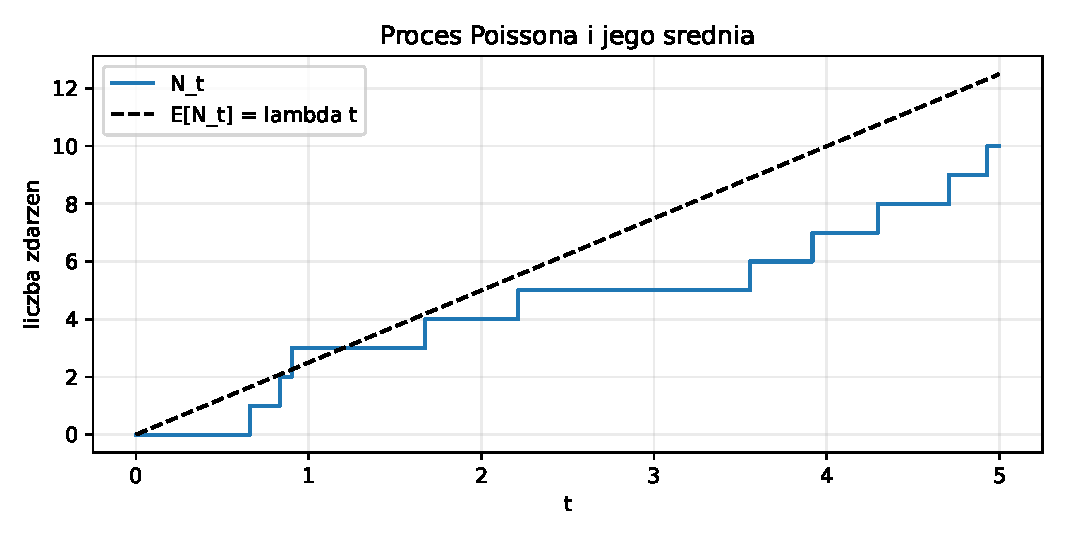
\includegraphics[width=0.88\textwidth]{figures/II_poisson.pdf}\par
\small\emph{Rysunek: Jedna trajektoria procesu Poissona i jej deterministyczna średnia.}
\end{center}
\noindent\textbf{Kod w Pythonie (NumPy, Matplotlib).} Plik \texttt{code/II\_poisson.py} można uruchomić niezależnie; zapisuje pokazany wykres.
\lstinputlisting[language=Python]{code/II_poisson.py}
\noindent\textbf{Odpowiednik w Julii (biblioteka standardowa).} Kod pokazuje to samo zjawisko w prostej symulacji.
\lstinputlisting[language=Julia]{code/II_julia_poisson.jl}
% --- KONIEC ROZSZERZENIA ILUSTRACYJNEGO ---

\section{Własność braku pamięci, filtracja i martyngał}\label{sec:volII:04:03}
\begin{stwierdzenie}[Brak pamięci rozkładu wykładniczego]\label{prop:volII:04:01}
Jeżeli $E\sim\operatorname{Exp}(\lambda)$, $\lambda>0$, to
$\Prob(E>s+t\mid E>s)=\Prob(E>t)$ dla wszystkich $s,t\ge0$.
Wśród rozkładów na $[0,\infty)$ o ciągłej funkcji przeżycia,
ściśle dodatniej dla argumentów skończonych i przyjmującej wartość
$1$ w zerze, ta własność charakteryzuje rozkład wykładniczy.
\end{stwierdzenie}
\begin{proof}
Pierwsza równość wynika ze wzoru
$e^{-\lambda(s+t)}/e^{-\lambda s}=e^{-\lambda t}$.
Dla odwrotnego kierunku oznaczmy $g(t)=\Prob(E>t)$.
Z własności warunkowania wynika $g(s+t)=g(s)g(t)$.
Funkcja $h(t):=-\log g(t)$ jest ciągła, spełnia równanie
$h(s+t)=h(s)+h(t)$ dla $s,t\ge0$ i $h(0)=0$.
Stąd najpierw dla argumentów wymiernych, a potem przez ciągłość
dla wszystkich $t\ge0$ otrzymujemy $h(t)=\lambda t$.
Ponieważ $g$ jest nierosnąca, $\lambda\ge0$; aby otrzymać
właściwy rozkład ze skończoną wartością $E$ prawie na pewno,
musimy mieć $\lim_{t\to\infty}g(t)=0$, a więc $\lambda>0$.
\end{proof}

\begin{twierdzenie}[Proces Poissona jest procesem Markowa]\label{thm:volII:04:03}
Niech $N$ będzie procesem Poissona o intensywności $\lambda>0$,
a $\calF_t^N:=\sigma(N_s:0\le s\le t)$ jego naturalną
filtracją. Dla $0\le s<t$ i każdego $k\in\N_0$ zachodzi
\[
\Prob(N_t=N_s+k\mid\calF_s^N)
=e^{-\lambda(t-s)}\frac{[\lambda(t-s)]^k}{k!}
\quad\text{prawie na pewno}.
\]
W szczególności rozkład przyszłego stanu warunkowo względem
całej przeszłości zależy wyłącznie od aktualnego $N_s$.
\end{twierdzenie}
\begin{proof}
Z twierdzenia~\ref{thm:poisson-fdd} wynika niezależność
$N_t-N_s$ od wszystkich wektorów
$(N_{u_1},\ldots,N_{u_r})$ z $u_j\le s$:
możemy każdy $N_{u_j}$ zapisać jako sumę przyrostów na podziale
przedziału $[0,s]$ zawierającym wszystkie $u_j$.
Klasa zdarzeń cylindrycznych wyznaczonych przez takie wektory
jest $\pi$-układem generującym $\calF_s^N$.
Przez twierdzenie o jednoznaczności miar (argument
$\pi$--$\lambda$) niezależność rozciąga się na całe
$\calF_s^N$. Zatem rozkład warunkowy przyrostu jest jego
rozkładem bezwarunkowym, wyliczonym wcześniej.
Ponieważ $N_t=N_s+(N_t-N_s)$, dostajemy tezę.
\end{proof}

\begin{wniosek}[Kompensowany proces Poissona]\label{cor:volII:04:01}
Dla procesu Poissona o intensywności $\lambda>0$ proces
$M_t:=N_t-\lambda t$ jest kwadratowalnym martyngałem względem
filtracji naturalnej $\mathbb F^N$, a
$\E(M_t-M_s)^2=\lambda(t-s)$ dla $0\le s\le t$.
\end{wniosek}
\begin{proof}
Dla $s\le t$ niezależność przyrostów daje
$\E[N_t-N_s\mid\calF_s^N]=\lambda(t-s)$,
więc $\E[M_t\mid\calF_s^N]=M_s$.
Całkowalność i kwadratowalność wynikają z momentów
rozkładu Poissona. Wreszcie
$\E(M_t-M_s)^2=\Var(N_t-N_s)=\lambda(t-s)$.
\end{proof}


\begin{center}
\begin{tikzpicture}[>=Latex,x=.95cm,y=.78cm]
\draw[->] (0,0)--(10,0) node[right] {$t$};
\foreach \x/\lab in {1/$T_1$,3/$T_2$,6/$T_3$,8/$T_4$}{
  \draw[red!65!black,very thick] (\x,-.16)--(\x,.16);
  \node[above=3pt] at (\x,.17) {\lab};
}
\draw[<->,blue!60!black] (1,-.52)--(3,-.52)
 node[midway,below] {$E_2=T_2-T_1$};
\draw[<->,blue!60!black] (3,-1.1)--(6,-1.1)
 node[midway,below] {$E_3=T_3-T_2$};
\node[align=left] at (5,1.05)
 {czasy nadejść: $T_1,T_2,\ldots$\qquad odstępy: $E_1,E_2,\ldots$};
\end{tikzpicture}
\par\smallskip\small Oś chwil nadejścia. Zliczenia na przedziale $(s,t]$
 zależą od liczby zaznaczonych punktów, a odstępy opisują
 czas pomiędzy kolejnymi punktami.
\end{center}

\section{Czasy nadejść i warunkowanie na liczbie zdarzeń}\label{sec:volII:04:04}
\begin{twierdzenie}[Chwila $n$-tego zdarzenia]\label{thm:volII:04:04}
Dla $n\ge1$ w procesie Poissona z intensywnością $\lambda>0$
czas $T_n$ ma rozkład gamma o parametrach $n$ i $\lambda$,
przy konwencji, że drugi parametr jest intensywnością. Zachodzi
\[
\Prob(T_n>t)=e^{-\lambda t}\sum_{k=0}^{n-1}
\frac{(\lambda t)^k}{k!},\qquad
\E T_n=\frac n\lambda,\qquad \Var(T_n)=\frac n{\lambda^2}.
\]
\end{twierdzenie}
\begin{proof}
Gęstość została wyprowadzona wcześniej. Zdarzenie
$\{T_n>t\}$ jest identyczne ze zdarzeniem $\{N_t\le n-1\}$;
stąd wzór na funkcję przeżycia. Ponieważ
$T_n=E_1+\cdots+E_n$, niezależność i momenty rozkładu
wykładniczego dają wskazane średnią i wariancję.
\end{proof}

\begin{twierdzenie}[Jednostajność chwil nadejść przy ustalonej liczbie]\label{thm:volII:04:05}
\label{thm:uniform-poisson-times}
Niech $t>0$ i $n\ge1$. Warunkowo względem zdarzenia
$\{N_t=n\}$ wektor $(T_1,\ldots,T_n)$ ma taki sam rozkład,
jak uporządkowane statystyki pozycyjne $n$ niezależnych
zmiennych o rozkładzie jednostajnym na $(0,t)$.
W szczególności dla $0<s<t$ i $0\le k\le n$
\[
\Prob(N_s=k\mid N_t=n)
=\binom nk\left(\frac{s}{t}\right)^k
\left(1-\frac{s}{t}\right)^{n-k}.
\]
\end{twierdzenie}
\begin{proof}
W dowodzie twierdzenia~\ref{thm:poisson-fdd} otrzymaliśmy
warunkową gęstość $n!/t^n$ na sympleksie
$0<s_1<\cdots<s_n<t$. Dokładnie taka jest gęstość
statystyk pozycyjnych z jednostajnego losowania
(gęstość wspólna nieuporządkowanego wektora to $t^{-n}$,
a każdy porządek z $n!$ ma jednakowe prawdopodobieństwo).
Liczba wylosowanych punktów należących do $(0,s]$ jest sumą
$n$ niezależnych zmiennych Bernoulliego z parametrem $s/t$,
co daje wzór dwumianowy.
\end{proof}

Warto zauważyć zmianę perspektywy: bez warunkowania liczby
nadejść w rozłącznych przedziałach są niezależne, ale po warunku
$N_t=n$ przestają być niezależne, bo ich suma musi wynosić $n$.

\begin{zadanie}[Cztery zgłoszenia w godzinę]
Zgłoszenia pojawiają się zgodnie z procesem Poissona o
intensywności $\lambda=4$ na godzinę. Obliczyć: (a)
prawdopodobieństwo dokładnie trzech zgłoszeń w pierwszej godzinie;
(b) prawdopodobieństwo, że do chwili $15$ minut nadejdzie
przynajmniej jedno zgłoszenie; (c) prawdopodobieństwo,
że przy dokładnie czterech zgłoszeniach w godzinie dwa z nich
wystąpiły w pierwszych piętnastu minutach;
(d) oczekiwany czas czwartego zgłoszenia.

\emph{Rozwiązanie.} Przyjmujemy czas w godzinach.
(a) Z rozkładu Poissona dostajemy
$\Prob(N_1=3)=e^{-4}4^3/3!$.
(b) Na odcinku $[0,1/4]$ oczekiwana liczba zgłoszeń wynosi
$1$, więc $\Prob(N_{1/4}\ge1)=1-e^{-1}$.
(c) Z twierdzenia~\ref{thm:uniform-poisson-times} liczba
zgłoszeń w pierwszym kwadransie pod warunkiem $N_1=4$
ma rozkład $\operatorname{Bin}(4,1/4)$; prawdopodobieństwo
wynosi $\binom42(1/4)^2(3/4)^2=27/128$.
(d) Suma czterech niezależnych odstępów wykładniczych ma średnią
$4/\lambda=1$ godzinę. Średnia ta nie oznacza oczywiście, że
czwarte zgłoszenie przychodzi dokładnie po godzinie.
\end{zadanie}


\begin{zadanie}[Dokładne chwile nadejść po warunkowaniu]
Klienci przybywają według procesu Poissona o intensywności
$\lambda>0$. Wiemy, że w ciągu dwóch godzin przybyło dokładnie
dwóch klientów. Niech $T_1<T_2$ będą ich chwilami przybycia.
Obliczyć $\Prob(T_1<1<T_2\mid N_2=2)$,
$\E[T_1\mid N_2=2]$ oraz gęstość wspólną $(T_1,T_2)$
przy tym warunku.

\emph{Rozwiązanie.} Warunkowo względem $N_2=2$
dwie chwile są statystykami pozycyjnymi dwóch niezależnych
zmiennych o rozkładzie jednostajnym na $[0,2]$.
Ich uporządkowana gęstość wynosi
$f(s_1,s_2)=\frac{2!}{2^2}=\frac12$ na trójkącie
$0<s_1<s_2<2$ i jest zerowa poza nim. Zdarzenie
$T_1<1<T_2$ oznacza, że jedna chwila znajduje się
w $(0,1)$, a druga w $(1,2)$; dlatego ma warunkowe
prawdopodobieństwo $2(1/2)^2=1/2$.
Dystrybuanta minimum dwóch zmiennych jednostajnych daje
$\Prob(T_1>u\mid N_2=2)=(1-u/2)^2$ dla $0\le u\le2$.
Stąd, całkując funkcję przeżycia,
\[
\E[T_1\mid N_2=2]
=\int_0^2(1-u/2)^2\,\dd u=\frac23.
\]
Wyniki nie zależą od $\lambda$: po ustaleniu liczby nadejść
intensywność nie wpływa na względne położenie ich chwil.
\end{zadanie}

\section{Superpozycja i rozrzedzanie}\label{sec:volII:04:05}
\begin{twierdzenie}[Superpozycja]\label{thm:volII:04:06}
Niech $N^{(1)},\ldots,N^{(r)}$ będą niezależnymi procesami
Poissona o intensywnościach $\lambda_1,\ldots,\lambda_r>0$.
Wtedy $N_t:=\sum_{j=1}^rN_t^{(j)}$ jest procesem Poissona
o intensywności $\lambda:=\sum_j\lambda_j$.
\end{twierdzenie}
\begin{proof}
Trajektorie sumy są niemalejące i prawostronnie ciągłe.
W ustalonej chwili prawdopodobieństwo jednoczesnego skoku
dwóch niezależnych procesów wynosi zero: warunkowo względem
skończonej liczby skoków pierwszego procesu na przedziale
$[0,m]$, ich chwile mają rozkład z gęstością;
dla każdej deterministycznej chwili prawdopodobieństwo skoku
drugiego procesu jest zero. Sumując po chwilach i po $m\in\N$,
wykluczamy wspólne skoki prawie na pewno.

Dla rozłącznych przedziałów przyrosty sumy są niezależne,
ponieważ wszystkie przyrosty procesów składowych z tych
przedziałów tworzą niezależną rodzinę. Dla pojedynczego
przedziału długości $h$ funkcja tworząca prawdopodobieństwa
przyrostu wynosi
\[
\E z^{\sum_j (N_{t+h}^{(j)}-N_t^{(j)})}
=\prod_j e^{\lambda_j h(z-1)}
=e^{(\sum_j\lambda_j)h(z-1)},\qquad 0\le z\le1.
\]
Jest to funkcja tworząca rozkładu
$\operatorname{Poisson}(\lambda h)$; jednoznaczność
współczynników szeregu potęgowego daje taki właśnie rozkład.
Zatem suma spełnia charakterystykę z twierdzenia
\ref{thm:poisson-fdd}.
\end{proof}

\begin{twierdzenie}[Niezależne rozrzedzanie]\label{thm:volII:04:07}
Niech $N$ będzie procesem Poissona o intensywności $\lambda>0$.
Każdy jego skok, niezależnie od innych skoków i od $N$,
oznaczmy jako typu $A$ z prawdopodobieństwem $p\in[0,1]$,
a jako typu $B$ z prawdopodobieństwem $1-p$.
Niech $N_t^A$ oraz $N_t^B$ zliczają odpowiednie typy do chwili $t$.
Wtedy $N^A$ i $N^B$ są \emph{niezależnymi} procesami Poissona
o intensywnościach $\lambda p$ i $\lambda(1-p)$
(z konwencją, że intensywność $0$ oznacza proces zerowy).
\end{twierdzenie}
\begin{proof}
Na ustalonym przedziale długości $h$, warunkowo względem
$N_{t+h}-N_t=n$, liczba oznaczeń $A$ ma rozkład
$\operatorname{Bin}(n,p)$, a liczba $B$ jest dopełnieniem do $n$.
Dla $|u|,|v|\le1$ wspólna funkcja tworząca wynosi
\[
\E\left[u^{N^A_{t+h}-N^A_t}v^{N^B_{t+h}-N^B_t}\right]
=\E[ (pu+(1-p)v)^{N_{t+h}-N_t}]
=e^{\lambda h p(u-1)}e^{\lambda h(1-p)(v-1)}.
\]
Iloczyn wskazuje jednocześnie rozkłady Poissona i
niezależność dwóch liczników na tym przedziale.
Ponieważ podstawowy proces ma niezależne przyrosty, a
oznaczenia na rozłącznych przedziałach są niezależne,
rozumowanie stosuje się łącznie do dowolnej skończonej
rodziny rozłącznych przedziałów. Tym samym oba powstałe
procesy są niezależne jako rodziny zmiennych losowych,
a nie tylko dla każdego ustalonego $t$.
\end{proof}

\begin{zadanie}[Dwa strumienie i klasyfikacja zgłoszeń]
Przychodzą niezależne zgłoszenia z działów $A$ i $B$
o intensywnościach odpowiednio $2$ i $3$ na godzinę.
Dodatkowo każde zgłoszenie, niezależnie od pozostałych, jest
pilne z prawdopodobieństwem $1/5$. Obliczyć
prawdopodobieństwo braku pilnych zgłoszeń w ciągu dwóch godzin;
oraz prawdopodobieństwo, że pierwsze zgłoszenie całego systemu
pochodzi z działu $A$.

\emph{Rozwiązanie.} Superpozycja daje intensywność $5$.
Rozrzedzenie pilnych zgłoszeń ma intensywność $5/5=1$;
w ciągu dwóch godzin liczba pilnych zgłoszeń jest więc
$\operatorname{Poisson}(2)$, a prawdopodobieństwo zera wynosi
$e^{-2}$.
Pierwsze czasy nadejść z działów $A$ i $B$ są niezależne,
$U\sim\operatorname{Exp}(2)$ i
$V\sim\operatorname{Exp}(3)$. Zatem
\[
\Prob(U<V)=\int_0^\infty \Prob(V>u)\,2e^{-2u}\,\dd u
=\int_0^\infty 2e^{-5u}\,\dd u=\frac25.
\]
Interpretacja: spośród wszystkich zdarzeń frakcja $2/5$
pochodzi średnio z działu $A$, ale wynikiem jest tu
konkretne prawdopodobieństwo typu \emph{pierwszego} zgłoszenia.
\end{zadanie}

\section{Złożony proces Poissona i kompensacja}\label{sec:volII:04:06}
\begin{definicja}[Złożony proces Poissona]\label{def:volII:04:03}
Niech $N$ będzie procesem Poissona o intensywności $\lambda>0$,
a $(Y_k)_{k\ge1}$ ciągiem niezależnych rzeczywistych
zmiennych losowych o wspólnym rozkładzie, niezależnym od $N$.
Definiujemy $S_t=\sum_{k=1}^{N_t}Y_k$,
gdzie pusta suma wynosi zero. Proces $S$ nazywamy
\emph{złożonym procesem Poissona}. Skok $S$ w chwili $T_k$
ma wielkość $Y_k$.
\end{definicja}

Model ma szerokie zastosowania: wypadki występują w chwilach
Poissona, natomiast kwota szkody jest niezależnym losowym
\emph{znacznikiem} zdarzenia. Dla $Y_k=1$ odzyskujemy $N_t$.

\begin{twierdzenie}[Moment, wariancja i funkcja charakterystyczna]\label{thm:volII:04:08}
Załóżmy w poprzedniej definicji $\E|Y_1|<\infty$.
Wtedy $\E S_t=\lambda t\E Y_1$.
Jeśli ponadto $\E Y_1^2<\infty$, to
$\Var(S_t)=\lambda t\E Y_1^2$.
Bez założeń momentowych zachodzi dla $u\in\R$
\[
\E e^{iuS_t}=\exp\!\bigl(\lambda t(\E e^{iuY_1}-1)\bigr).
\]
Przy $\E|Y_1|<\infty$ proces
$S_t-\lambda t\E Y_1$ jest martyngałem względem
filtracji generowanej przez zaznaczone zdarzenia do chwili $t$.
\end{twierdzenie}
\begin{proof}
Warunkując względem $N_t=n$ i używając niezależności znaczników,
uzyskujemy $\E[S_t\mid N_t=n]=n\E Y_1$,
$\Var(S_t\mid N_t=n)=n\Var(Y_1)$ i
$\E[e^{iuS_t}\mid N_t=n]=(\E e^{iuY_1})^n$.
Po uśrednieniu pierwsza równość jest oczywista. Ze wzoru
na wariancję całkowitą wynika
\begin{align*}
\Var(S_t)&=\E[N_t\Var(Y_1)]
 +\Var(N_t\E Y_1)\\
&=\lambda t\bigl(\Var(Y_1)+(\E Y_1)^2\bigr)
=\lambda t\E Y_1^2.
\end{align*}
Uśrednienie funkcji charakterystycznej wykorzystuje szereg
$\sum_{n\ge0}e^{-\lambda t}(\lambda t)^n z^n/n!
=e^{\lambda t(z-1)}$.
Przyrosty $S_t-S_s$ są niezależne od informacji do chwili $s$
i mają średnią $\lambda(t-s)\E Y_1$:
wynika to z niezależnych przyrostów procesu Poissona i z faktu,
że znaczniki przyszłych zdarzeń są niezależne od przeszłych.
Stąd właściwość martyngałowa po odjęciu deterministycznej średniej.
\end{proof}

\section{Niejednorodny proces Poissona}\label{sec:volII:04:07}
Stała intensywność jest wygodna, ale liczba zgłoszeń w ciągu
dnia na ogół zależy od godziny. Następująca konstrukcja pokazuje,
że zmienna intensywność nie wymaga zmiany podstawowych idei.

\begin{definicja}[Proces Poissona z deterministyczną intensywnością]\label{def:volII:04:04}
Niech $a:[0,\infty)\to[0,\infty)$ będzie funkcją borelowską,
całkowalną na każdym przedziale $[0,t]$. Oznaczmy
$A(t)=\int_0^t a(s)\,\dd s$.
Jeżeli $\widetilde N$ jest standardowym procesem Poissona
o intensywności $1$, to proces $N_t=\widetilde N_{A(t)}$
nazywamy \emph{niejednorodnym procesem Poissona o intensywności $a$}.
\end{definicja}

\begin{stwierdzenie}\label{prop:volII:04:02}
Dla procesu z poprzedniej definicji i $0\le s<t$ przyrost
$N_t-N_s$ ma rozkład
$\operatorname{Poisson}(\int_s^t a(u)\,\dd u)$, a przyrosty
na rozłącznych przedziałach są niezależne. Ponadto
$\Prob(N_t-N_s=0)=\exp(-\int_s^t a(u)\,\dd u)$.
\end{stwierdzenie}
\begin{proof}
Funkcja $A$ jest ciągła i niemalejąca, a
$A(t)-A(s)=\int_s^t a(u)\,\dd u$.
Stąd $N_t-N_s=\widetilde N_{A(t)}-\widetilde N_{A(s)}$.
Przedziały obrazowe $[A(s),A(t)]$ odpowiadające rozłącznym
przedziałom czasu mają rozłączne wnętrza; przedziały o
zerowej długości dają zerowe przyrosty. Zatem po zastosowaniu
niezależnych i stacjonarnych przyrostów $\widetilde N$
dostajemy wszystkie tezy.
\end{proof}

\begin{przyklad}[Intensywność sezonowa]
Niech $a(t)=2+t$ dla $0\le t\le2$ i $a(t)=4$ dla $t>2$.
W ciągu pierwszej godziny średnia liczba zdarzeń wynosi
$A(1)=\int_0^1(2+s)\,\dd s=5/2$,
a prawdopodobieństwo braku zgłoszeń jest $e^{-5/2}$.
Pomiędzy godziną pierwszą a drugą średnia przyrostu
wynosi $A(2)-A(1)=7/2$. Obie liczby zdarzeń są niezależne,
choć ich rozkłady nie są jednakowe: przyrosty pozostają
niezależne, ale przestają być stacjonarne.
\end{przyklad}

\section{Charakterystyka przez przyrosty i zdarzenia rzadkie}\label{sec:volII:04:08}
Dotychczas budowaliśmy proces Poissona z czasów wykładniczych.
Można jednak rozpocząć od modelowania zliczeń w krótkich
przedziałach. Poniższy wynik uzasadnia tę drogę konstrukcji.

\begin{twierdzenie}[Charakterystyka procesu Poissona przez małe przyrosty]\label{thm:volII:04:09}
\label{thm:poisson-infinitesimal}
Niech $N=(N_t)_{t\ge0}$ będzie procesem o wartościach
w $\N_0$, $N_0=0$, z niezależnymi i stacjonarnymi
nieujemnymi przyrostami. Załóżmy, że istnieje $\lambda>0$
takie, iż przy $h\downarrow0$
\[
\Prob(N_h=1)=\lambda h+o(h),\qquad
\Prob(N_h\ge2)=o(h).
\]
Wtedy dla każdego $t\ge0$ zachodzi
$N_t\sim\operatorname{Poisson}(\lambda t)$,
a rozkłady skończeniewymiarowe $N$ są takie same jak
rozkłady procesu Poissona o intensywności $\lambda$.
Jeżeli ponadto $N$ ma niemalejące trajektorie c\`adl\`ag,
to proces ten ma prawo procesu Poissona także jako
zmienna losowa w przestrzeni trajektorii c\`adl\`ag.
\end{twierdzenie}
\begin{proof}
Ustalmy $z\in[0,1]$ i funkcję tworzącą
$G_t(z)=\E z^{N_t}$, przyjmując $0^0=1$.
Z niezależnych i stacjonarnych przyrostów wynika
$G_{t+h}(z)=G_t(z)G_h(z)$. Ponieważ
$\Prob(N_h=0)=1-\lambda h+o(h)$, a wkład stanów
$N_h\ge2$ do $G_h(z)$ ma moduł nie większy niż
$\Prob(N_h\ge2)=o(h)$, otrzymujemy
\[
G_h(z)=1+\lambda h(z-1)+o(h).
\]
Zatem dla $t\ge0$ pochodna prawostronna spełnia
\[
\frac{\partial}{\partial t^+}G_t(z)
=\lim_{h\downarrow0}G_t(z)\frac{G_h(z)-1}{h}
=\lambda(z-1)G_t(z).
\]
Dodatkowo z $\Prob(N_h=0)\to1$ oraz niezależnych przyrostów
wynika ciągłość $t\mapsto G_t(z)$: z prawej na mocy
$G_{t+h}=G_tG_h$, a z lewej, dla $0<h\le t$,
$G_t=G_{t-h}G_h$ i $G_h\to1$; ponieważ
$0\le G_{t-h}\le1$, różnica dąży do zera.
Funkcja ciągła z ciągłą pochodną prawostronną zadaną
powyższym równaniem ma jego zwykłe rozwiązanie,
co można sprawdzić dla
$H_t=e^{-\lambda(z-1)t}G_t(z)$:
jej pochodna prawostronna znika w każdym punkcie,
a więc $H$ jest stała (wynika to z twierdzenia
o wartości średniej w wersji dla pochodnych jednostronnych,
lub z zastosowania argumentu o ekstremum do
$H_t\pm\varepsilon t$). Ponieważ $G_0(z)=1$,
\[
G_t(z)=e^{\lambda t(z-1)}.
\]
Współczynniki szeregu potęgowego są równe
$e^{-\lambda t}(\lambda t)^n/n!$, co daje rozkład Poissona.
Ponieważ przyrosty są niezależne i stacjonarne,
wszystkie rozkłady skończeniewymiarowe są wyznaczone
przez właśnie otrzymane rozkłady pojedynczych przyrostów.
Dla procesów c\`adl\`ag na przestrzeni $D([0,\infty),\N_0)$
rozkłady skończeniewymiarowe wyznaczają prawo procesu
(jego borelowską $\sigma$-algebrę generują współrzędne),
co kończy dowód.
\end{proof}

\begin{przyklad}[Rozrzedzony schemat Bernoulliego]
Ustalmy $t>0$ i rozważmy $m$ niezależnych prób
na siatce $t/m,2t/m,\ldots,t$, z prawdopodobieństwem
sukcesu $\lambda t/m$ w każdej próbie (dla dostatecznie
dużych $m$). Liczba sukcesów ma rozkład
$\operatorname{Bin}(m,\lambda t/m)$.
Dla ustalonego $k\ge0$ jej prawdopodobieństwo wynosi
\[
\binom mk\left(\frac{\lambda t}{m}\right)^k
\left(1-\frac{\lambda t}{m}\right)^{m-k}
\longrightarrow e^{-\lambda t}\frac{(\lambda t)^k}{k!}.
\]
Granica wynika z
$\binom mk/m^k\to1/k!$ i
$(1-\lambda t/m)^m\to e^{-\lambda t}$.
Dla wszystkich rozłącznych odcinków siatki liczby
sukcesów są niezależne; analogicznie otrzymujemy
zbieżność ich wspólnych rozkładów do niezależnych
przyrostów Poissona. Jest to matematyczne wyjaśnienie,
dlaczego rozkład Poissona naturalnie opisuje wiele
niezależnych, rzadkich zdarzeń.
\end{przyklad}

\section{Co wynika z modelu, a czego model nie mówi?}\label{sec:volII:04:09}
Rozkład Poissona nie jest uniwersalnym opisem każdego
zliczania. Jeśli nadejście klienta zwiększa lub zmniejsza
szansę kolejnego nadejścia, niezależność przyrostów jest
nieadekwatna. Jeśli urządzenie ma okres refrakcji, to
bardzo krótkie odstępy między zdarzeniami nie są wykładnicze.
Na dalszych stronach uogólnimy ideę zliczania przez
\emph{intensywności zależne od stanu}. Otrzymamy łańcuchy
Markowa w czasie ciągłym, których czasy oczekiwania będą
nadal wykładnicze, ale ich parametry będą zmieniać się
po każdym skoku procesu.
% ================================================================
% TOM II. ROZDZIAŁ 5
% ================================================================
\chapter{Łańcuchy Markowa w czasie ciągłym}
\label{chap:volII:05}
\par\smallskip\noindent{\small\textit{Powiązania:} \textup{tom~I}, sekcja~\ref{I-sec:volI:12:02} (łańcuchy dyskretne); sekcja~\ref{sec:volII:04:02} (zegar Poissona); \textup{tom~III}, sekcja~\ref{III-sec:volIII:06:03} (generator dyfuzji); tom~I, twierdzenie~\ref{I-thm:volI:12:07} (mocna własność Markowa).}\par\smallskip

\label{ch:ctmc}

\section{Dlaczego macierz przejścia nie wystarcza?}\label{sec:volII:05:01}
W łańcuchu Markowa z czasu dyskretnego macierz $P=(p_{ij})$
opisuje jeden krok. W czasie ciągłym pojawiają się dwie odrębne
losowości: \emph{kiedy} następuje zmiana stanu oraz \emph{dokąd}
proces przechodzi. W modelu awarii i naprawy urządzenie może długo
pozostawać sprawne, a po awarii przebywać w stanie uszkodzenia
przez losowy czas. Sam ciąg odwiedzanych stanów nie opisuje
czasów trwania poszczególnych faz.

\begin{definicja}[Macierz intensywności]\label{def:volII:05:01}
Niech $E$ będzie skończonym lub przeliczalnym zbiorem stanów.
\emph{Konserwatywną macierzą intensywności} (macierzą $Q$)
nazywamy macierz $Q=(q_{ij})_{i,j\in E}$ spełniającą:
$q_{ij}\ge0$ dla $i\ne j$, $q_i:=-q_{ii}\in[0,\infty)$
oraz $\sum_{j\ne i}q_{ij}=q_i$ dla każdego $i\in E$.
Gdy $q_i>0$, definiujemy prawdopodobieństwa skoku
$r_{ij}=q_{ij}/q_i$ dla $j\ne i$ i $r_{ii}=0$.
Stan z $q_i=0$ jest pochłaniający.
\end{definicja}

Wyraz $q_{ij}$, $i\ne j$, jest natężeniem \emph{bezpośredniego}
przejścia z $i$ do $j$, a $q_i$ całkowitą intensywnością
opuszczenia stanu $i$. Zapis $q_{ii}=-q_i$ nie oznacza
ujemnego prawdopodobieństwa: elementy macierzy $Q$ są
intensywnościami, a nie prawdopodobieństwami.

\begin{przyklad}[Układ sprawny--uszkodzony]
Niech $E=\{0,1\}$, gdzie $0$ oznacza urządzenie sprawne,
a $1$ uszkodzone. Jeśli awarie występują z intensywnością
$\alpha>0$, a zakończenia napraw z intensywnością $\beta>0$,
to
\[
Q=\begin{pmatrix}-\alpha&\alpha\\\beta&-\beta\end{pmatrix}.
\]
Czas do awarii, rozpoczynając od stanu $0$, ma rozkład
$\operatorname{Exp}(\alpha)$; czas naprawy w stanie $1$
ma rozkład $\operatorname{Exp}(\beta)$. Po każdym przejściu
zaczyna się nowy, niezależny czas oczekiwania.
\end{przyklad}

\begin{center}
\begin{tikzpicture}[>=Latex,thick,node distance=2.4cm,
 st/.style={draw,circle,minimum size=11mm,fill=blue!5}]
\node[st] (zero) {$0$};
\node[st,right=of zero] (one) {$1$};
\node[st,right=of one] (two) {$2$};
\draw[->,bend left=22] (zero) to node[above] {$q_{01}=2$} (one);
\draw[->,bend left=22] (one) to node[below] {$q_{10}=1$} (zero);
\draw[->] (one) -- node[above] {$q_{12}=3$} (two);
\node[below=9mm of two] {pochłanianie};
\end{tikzpicture}
\par\smallskip\small Schemat: intensywności skoków dla trzech stanów.
W stanie $1$ łączna intensywność wynosi $1+3=4$.
\end{center}


\begin{uwaga}[Czym macierz intensywności różni się od macierzy przejścia?]
Jeżeli proces zaczyna w stanie $i$, to dla $j\ne i$
$\Prob_i(X_h=j)=q_{ij}h+O(h^2)$ przy $h\downarrow0$
\emph{w skończonym modelu}. Tymczasem dla dowolnego
ustalonego $t>0$ prawdopodobieństwo $p_{ij}(t)$ może zawierać
wkład wielu następujących po sobie zmian stanu.
Zatem $q_{ij}$ nie jest ani prawdopodobieństwem pojedynczego
skoku (nim jest $q_{ij}/q_i$), ani prawdopodobieństwem
znalezienia się w $j$ po czasie $t$ (nim jest $p_{ij}(t)$).
\end{uwaga}

\section{Konstrukcja przez łańcuch skoków i czasy przebywania}\label{sec:volII:05:02}
\begin{twierdzenie}[Konstrukcja minimalnego procesu skokowego]\label{thm:volII:05:01}
\label{thm:jump-construction}
Niech $E$ będzie zbiorem przeliczalnym, $Q$ konserwatywną
macierzą intensywności z $q_i<\infty$ dla każdego $i\in E$,
a $\mu$ rozkładem probabilistycznym na $E$.
Istnieje przestrzeń probabilistyczna, na której można
zdefiniować ciąg stanów $Y_0,Y_1,\ldots$, ciąg czasów skoków
$0=J_0<J_1<\cdots$ aż do ewentualnego pochłonięcia oraz
proces $X$ następująco:
\begin{itemize}
\item $Y_0\sim\mu$, a ze stanu $i$ o $q_i>0$ następny stan
ma rozkład $(r_{ij})_{j\in E}$;
\item przy wejściu do $i$ o $q_i>0$ losujemy niezależny
czas przebywania o rozkładzie $\operatorname{Exp}(q_i)$;
\item dla $J_n\le t<J_{n+1}$ ustalamy $X_t=Y_n$,
a po wejściu do stanu z $q_i=0$ proces pozostaje w nim na stałe.
\end{itemize}
Jeśli suma wszystkich kolejnych czasów przebywania jest skończona,
jej granicę $\zeta$ nazywamy \emph{czasem eksplozji}; dla $t\ge\zeta$
ustalamy $X_t=\partial$ w dodatkowym stanie cmentarnym
$\partial\notin E$. Tak otrzymany proces nazywamy
\emph{minimalnym procesem skokowym o macierzy $Q$}.
Na przedziale $[0,\zeta)$ jego trajektorie są schodkowe i
c\`adl\`ag, a skoki mają czasy bez atomów.
\end{twierdzenie}
\begin{proof}
Dla każdego stanu $i$ z $q_i>0$ wiersz $(r_{ij})$ jest
rozkładem probabilistycznym. Używając niezależnych zmiennych
jednostajnych na $(0,1)$ oraz ustalonego wyliczenia stanów,
możemy metodą odwrotnej dystrybuanty wylosować następny stan
z tego rozkładu. Pozwala to rekurencyjnie skonstruować
$Y_0,Y_1,\ldots$; po pochłonięciu kończymy konstrukcję.

Niezależnie losujemy ciąg $Z_0,Z_1,\ldots$ o rozkładzie
$\operatorname{Exp}(1)$, a czas przebywania przy wizycie
w stanie $Y_n=i$ definiujemy jako $H_n=Z_n/q_i$.
Z równości
$\Prob(Z_n/q_i>t)=e^{-q_i t}$ wynika żądany rozkład
warunkowy. Ustalamy $J_{n+1}=J_n+H_n$ tak długo, jak
$Y_n$ nie jest stanem pochłaniającym.

Jeśli $J_n\uparrow\zeta<\infty$, to przed chwilą $\zeta$
występuje nieskończenie wiele skoków. Nie należy wtedy
arbitralnie przedłużać trajektorii w $E$, bo może ona nie
mieć granicy. Dodanie stanu $\partial$ daje jednoznaczny
minimalny proces do końca czasu. Każdy $H_n>0$, więc
poszczególne chwile $J_n$ są ściśle rosnące; na $[0,\zeta)$
na każdym przedziale domkniętym zawartym w $[0,\zeta)$
występuje tylko skończenie wiele skoków. Stąd wskazana
regularność trajektorii przed eksplozją.
\end{proof}

\begin{uwaga}[Dwie różne macierze]
Macierz $R=(r_{ij})$ opisuje \emph{dokąd} idziemy po skoku.
Macierz $Q$ opisuje łącznie wybór nowego stanu i tempo
opuszczania poprzedniego. Nawet jeśli dwa procesy mają taki sam
łańcuch skoków $Y_n$, lecz różne intensywności $q_i$,
mają inne rozkłady $X_t$ w czasie kalendarzowym.
\end{uwaga}


\begin{przyklad}[Dlaczego rozkład wykładniczy jest naturalny dla jednorodnego łańcucha?]
Przypuśćmy, że układ zaczyna w stanie $0$, czeka losowy
czas $H$, a następnie nieodwracalnie przechodzi do $1$.
Jeżeli $H\sim\operatorname{U}([0,2])$, to przy $0<s<s+h<2$
\[
\Prob(H>s+h\mid H>s)=\frac{2-s-h}{2-s}.
\]
To prawdopodobieństwo zależy od czasu $s$, który upłynął
od uruchomienia. Dla procesu, który \emph{jednorodnie}
zachowuje się w stanie $0$, oczekiwalibyśmy natomiast,
aby przy obecnym stanie $0$ szansa pozostania w nim przez
kolejne $h$ jednostek czasu nie zależała od wieku pobytu
w tym stanie. Gdy $H\sim\operatorname{Exp}(q)$, rzeczywiście
\[
\Prob(H>s+h\mid H>s)=e^{-qh}.
\]
Równanie braku pamięci wyjaśnia, dlaczego w konstrukcji
jednorodnego łańcucha Markowa wybieramy czasy wykładnicze.
Przy innych prawach czasu przebywania można otrzymać
\emph{proces pół-Markowa}, w którym do stanu należy
dodać informację o czasie od ostatniej zmiany.
\end{przyklad}

\section{Eksplozja i jej wykluczanie}\label{sec:volII:05:03}
\begin{twierdzenie}[Ograniczone intensywności wykluczają eksplozję]\label{thm:volII:05:02}
\label{thm:bounded-rates}
Niech proces minimalny z twierdzenia~\ref{thm:jump-construction}
ma $\sup_{i\in E}q_i\le\Lambda<\infty$.
Wtedy $\Prob(\zeta=\infty)=1$.
\end{twierdzenie}
\begin{proof}
Jeżeli proces wchodzi do stanu pochłaniającego, to oczywiście
nie może mieć nieskończenie wielu rzeczywistych skoków
w czasie skończonym. W przeciwnym razie kolejne czasy
przebywania są równe $H_n=Z_n/q_{Y_n}$, gdzie
$Z_n$ są niezależne o rozkładzie $\operatorname{Exp}(1)$.
Ponieważ $q_{Y_n}\le\Lambda$, mamy
$H_n\ge Z_n/\Lambda$ prawie na pewno.
Z lematu o braku eksplozji dla niezależnych wykładniczych
z rozdziału 4 wynika $\sum_n Z_n/\Lambda=\infty$
prawie na pewno. Także $\sum_n H_n=\infty$.
\end{proof}

\begin{przyklad}[Dlaczego skończoność każdego $q_i$ nie wystarcza?]
Niech $E=\N_0$, a jedyne dozwolone przejście ma postać
$n\to n+1$ z intensywnością $q_{n,n+1}=\lambda_n>0$.
Czas eksplozji jest sumą niezależnych zmiennych
$H_n\sim\operatorname{Exp}(\lambda_n)$.
Dla $\lambda_n=(n+1)^2$ mamy
\[
\E\zeta=\sum_{n=0}^\infty\frac1{(n+1)^2}<\infty.
\]
Ponieważ $\zeta\ge0$, skończona wartość oczekiwana
implikuje $\zeta<\infty$ prawie na pewno.
Nieskończenie wiele skoków występuje więc przed pewną
skończoną, losową chwilą! To model eksplozji.
Natomiast dla $\lambda_n=n+1$ zbieżność $\sum1/\lambda_n$
nie zachodzi; poniższe twierdzenie pokazuje brak eksplozji.
\end{przyklad}

\begin{twierdzenie}[Kryterium eksplozji procesu czystych urodzin]\label{thm:volII:05:03}
\label{thm:pure-birth-explosion}
Niech $E=\N_0$, $X_0=0$, a jedyną możliwą zmianą stanu
$n$ będzie przejście do $n+1$ z intensywnością
$\lambda_n\in(0,\infty)$. Wówczas
\[
\Prob(\zeta<\infty)=1
\quad\Longleftrightarrow\quad
\sum_{n=0}^\infty\frac1{\lambda_n}<\infty.
\]
Jeśli szereg jest rozbieżny, to $\Prob(\zeta=\infty)=1$.
\end{twierdzenie}
\begin{proof}
Mamy $\zeta=\sum_{n\ge0}H_n$ z niezależnymi
$H_n\sim\operatorname{Exp}(\lambda_n)$.
Jeżeli $\sum1/\lambda_n<\infty$, to
$\E\zeta=\sum\E H_n<\infty$ na mocy twierdzenia o
zbieżności monotonicznej, skąd $\zeta<\infty$ prawie na pewno.

Załóżmy teraz $\sum1/\lambda_n=\infty$.
Dla $c>0$ niezależność i zbieżność ograniczona dają
\[
\E e^{-c\zeta}
=\lim_{m\to\infty}\prod_{n=0}^m\E e^{-cH_n}
=\prod_{n=0}^\infty\frac{\lambda_n}{\lambda_n+c}.
\]
Musimy pokazać, że iloczyn jest zerowy. Jego ujemny logarytm
to szereg $\sum_n\log(1+c/\lambda_n)$.
Jeśli nieskończenie wiele $\lambda_n\le c$, to w szeregu
nieskończenie wiele wyrazów jest nie mniejszych od $\log2$.
W przeciwnym razie dla wszystkich dostatecznie dużych $n$
mamy $0<c/\lambda_n<1$, a więc
$\log(1+c/\lambda_n)\ge c/(2\lambda_n)$.
W obu przypadkach szereg logarytmów jest rozbieżny.
Zatem $\E e^{-c\zeta}=0$.
Przy przyjętej konwencji $e^{-c\infty}=0$, a dla każdej
skończonej wartości $\zeta$ wykładnik jest ściśle dodatni.
Stąd $\Prob(\zeta<\infty)=0$, co kończy dowód.
\end{proof}

\section{Macierz przejścia i równania Kołmogorowa}\label{sec:volII:05:04}
Teraz ograniczymy się do \emph{skończonej} przestrzeni $E$.
Założenie jest istotne: w nieskończonym zbiorze stanów
potrzebujemy dodatkowej kontroli, aby uzasadniać różniczkowanie
nieskończonych szeregów i wykluczać eksplozję.

\begin{definicja}[Macierz przejścia w czasie ciągłym]\label{def:volII:05:02}
Niech $E$ będzie skończone, a $X$ procesem o intensywnościach
$Q$. Dla $i,j\in E$ i $t\ge0$ definiujemy
$p_{ij}(t)=\Prob(X_t=j\mid X_0=i)$,
przy czym po prawej stronie rozumiemy prawo procesu
\emph{uruchomionego ze stanu $i$}, również wtedy,
gdy w wyjściowym rozkładzie początkowym $\Prob(X_0=i)=0$.
Macierz $P(t)=(p_{ij}(t))_{i,j\in E}$ nazywamy
\emph{macierzą przejścia w czasie $t$}.
\end{definicja}

\section{Zegar Poissona i uniformizacja}\label{sec:volII:05:05}
Najwygodniejsza metoda konstrukcji skończonego łańcucha
pozwala zarazem udowodnić równania różniczkowe macierzy
przejścia bez odwoływania się do formalnej ``rachunkowości
prawdopodobieństw $o(h)$''.

\begin{twierdzenie}[Uniformizacja]\label{thm:volII:05:04}
\label{thm:uniformization}
Niech $E$ będzie niepustym zbiorem skończonym,
a $Q$ konserwatywną macierzą intensywności.
Wybierzmy $\Lambda>\max_{i\in E}q_i$ i ustalmy
$R:=I+Q/\Lambda$. Wtedy $R$ jest macierzą stochastyczną.
Niech $(Y_n)_{n\ge0}$ będzie łańcuchem dyskretnym o macierzy
przejścia $R$, niezależnym od procesu Poissona $N$ o intensywności
$\Lambda$. Proces $X_t:=Y_{N_t}$ jest łańcuchem w czasie
ciągłym o intensywnościach $Q$, a jego macierz przejścia wynosi
\[
P(t)=e^{-\Lambda t}\sum_{n=0}^\infty
\frac{(\Lambda t)^n}{n!}R^n=e^{tQ},\qquad t\ge0.
\]
Dla każdego $i\ne j$ zachodzi
$\lim_{h\downarrow0}p_{ij}(h)/h=q_{ij}$,
a dla $i=j$ zachodzi
$\lim_{h\downarrow0}(p_{ii}(h)-1)/h=q_{ii}$.
\end{twierdzenie}
\begin{proof}
Dla $i\ne j$ mamy $R_{ij}=q_{ij}/\Lambda\ge0$,
a na przekątnej $R_{ii}=1-q_i/\Lambda>0$.
Suma każdego wiersza jest równa
$1+\Lambda^{-1}\sum_j q_{ij}=1$.
Wprowadzamy niezależny łańcuch skoków i zegar Poissona.
W chwili zegara $Y$ dokonuje kroku macierzy $R$; może
przy tym pozostać w obecnym stanie. Te pozorne skoki
nazywamy \emph{skokami fikcyjnymi}.

Warunkowo względem $N_t=n$ końcowy stan procesu ma
rozkład $n$-krokowy $R^n$. Dlatego
$P(t)=\sum_n\Prob(N_t=n)R^n$, czyli pierwsza suma.
Ponieważ $I$ i $R$ komutują,
\[
e^{-\Lambda t}\sum_{n=0}^\infty\frac{(\Lambda tR)^n}{n!}
=e^{-\Lambda t I}e^{\Lambda tR}
=e^{\Lambda t(R-I)}=e^{tQ}.
\]
Zbieżność jest bezproblemowa w skończonym wymiarze.
Rozwinięcie wykładnika macierzowego
$e^{hQ}=I+hQ+O(h^2)$ przy $h\downarrow0$
daje oba wskazane limity.

Pozostaje zweryfikować, że opis intensywności jest właściwy.
Będąc w stanie $i$, na krótkim przedziale $[t,t+h]$
występuje jeden impuls zegara z prawdopodobieństwem
$\Lambda h+O(h^2)$, dwa lub więcej z prawdopodobieństwem
$O(h^2)$, a pojedynczy impuls kieruje nas z $i$ do $j\ne i$
z prawdopodobieństwem $R_{ij}$. Zatem
$\Prob(X_{t+h}=j\mid X_t=i)=\Lambda hR_{ij}+O(h^2)
=q_{ij}h+O(h^2)$.
Łączna intensywność rzeczywistego opuszczenia $i$ jest
$\Lambda(1-R_{ii})=q_i$. Po każdym fikcyjnym kroku bez
zmiany stanu pozostajemy w $i$; własność braku pamięci
zegara Poissona daje wykładniczy czas do pierwszego
rzeczywistego skoku z parametrem $q_i$, a przy tym
prawdopodobieństwo jego kierunku to
$R_{ij}/(1-R_{ii})=q_{ij}/q_i$.
Jest to dokładnie konstrukcja procesu z $Q$.
\end{proof}


\begin{uwaga}[Dlaczego fikcyjne impulsy nie zmieniają modelu?]
Jeżeli proces zaczyna w stanie $i$ z $q_i>0$,
liczba impulsów fikcyjnych przed pierwszą rzeczywistą
zmianą stanu jest geometryczna. Można obliczyć
prawdopodobieństwo pozostawania w $i$ \emph{bez
rzeczywistego skoku} do chwili $t$ bez powoływania się
jedynie na intuicję pamięci rozkładu wykładniczego:
\[
\sum_{n=0}^\infty\Prob(N_t=n)R_{ii}^{n}
=e^{-\Lambda t}\exp(\Lambda tR_{ii})
=e^{-q_it}.
\]
Tak otrzymujemy czas oczekiwania $\operatorname{Exp}(q_i)$.
Warunkowo względem tego, że impuls powoduje rzeczywisty skok,
prawdopodobieństwo wybrania stanu $j\ne i$ jest
$R_{ij}/(1-R_{ii})=q_{ij}/q_i$.
Po skoku niezależne przyszłe impulsy zegara i kroki pomocnicze
pozwalają powtórzyć argument. Ta obserwacja uzasadnia
równoważność uniformizacji i konstrukcji przez czasy przebywania.
\end{uwaga}

Ważna korzyść uniformizacji jest obliczeniowa: możemy
symulować jeden wspólny zegar Poissona i niezależną sekwencję
kroków macierzy $R$, a przy prawdopodobieństwach przejścia
stosować nieujemny szereg zamiast bezpośrednio obliczać
wykładnik macierzowy.

\begin{twierdzenie}[Równania Chapmana--Kołmogorowa i Kołmogorowa]\label{thm:volII:05:05}
\label{thm:kolmogorov-eq}
Dla skończonej przestrzeni stanów i konserwatywnej macierzy
intensywności $Q$ macierz przejścia $P(t)=e^{tQ}$ spełnia
$P(0)=I$ i $P(t+s)=P(t)P(s)$ dla $s,t\ge0$. Ponadto
jest różniczkowalna dla każdego $t\ge0$ (w zerze prawostronnie)
i spełnia \emph{równanie wsteczne} oraz \emph{równanie w przód}:
\[
P'(t)=QP(t),\qquad P'(t)=P(t)Q.
\]
Współrzędnie, dla każdego $i,j\in E$,
\[
\frac{\dd}{\dd t}p_{ij}(t)=\sum_{k\in E}q_{ik}p_{kj}(t),
\qquad
\frac{\dd}{\dd t}p_{ij}(t)=\sum_{k\in E}p_{ik}(t)q_{kj}.
\]
\end{twierdzenie}
\begin{proof}
Wzór $P(t)=e^{tQ}$ otrzymaliśmy z konstrukcji, zatem
$P(t+s)=e^{(t+s)Q}=e^{tQ}e^{sQ}$.
Istnieje też interpretacja probabilistyczna: warunkujemy
stan w chwili $t$ i sumujemy po wszystkich stanach
pośrednich $k$, otrzymując
$p_{ij}(t+s)=\sum_kp_{ik}(t)p_{kj}(s)$.
Ponieważ wykładnik macierzowy jest szeregiem potęgowym
zbieżnym jednostajnie na przedziałach ograniczonych,
można go różniczkować wyraz po wyrazie; dostajemy
$P'(t)=Qe^{tQ}=e^{tQ}Q$.
Przemienność $Q$ z własnym wykładnikiem wynika również
bezpośrednio z definicji szeregu.
Zapisując mnożenie macierzy współrzędnie, uzyskujemy
obydwa wzory skalarne.
\end{proof}

\begin{uwaga}[Dlaczego są dwa równania?]
Równanie wsteczne analizuje \emph{pierwszą decyzję po starcie}:
pierwszy indeks $i$ należy do stanu startowego.
Równanie w przód analizuje \emph{dopływ do stanu końcowego}:
drugi indeks $j$ jest stanem w chwili $t$.
W skończonym jednorodnym modelu obydwa równania są poprawne
i prowadzą do tej samej macierzy. Dla modeli z nieskończenie
wieloma stanami albo z eksplozją przejścia do różniczkowania
w nieskończonych szeregach wymagają osobnego dowodu.
\end{uwaga}


\begin{przyklad}[Powrót do stanu początkowego to nie brak skoku]
W modelu $E=\{0,1\}$ z intensywnościami
$0\to1$ równą $\alpha>0$ i $1\to0$ równą $\beta>0$
czas do pierwszego \emph{rzeczywistego} skoku, przy starcie
z $0$, ma rozkład $\operatorname{Exp}(\alpha)$. Zatem
\[
\Prob_0(\text{brak skoku do }t)=e^{-\alpha t}.
\]
Natomiast $p_{00}(t)=\Prob_0(X_t=0)$ uwzględnia również
ścieżki z dwoma, czterema lub większą parzystą liczbą skoków.
W istocie, z rozwiązania równań w następnym podrozdziale,
\[
 p_{00}(t)=\frac{\beta+\alpha e^{-(\alpha+\beta)t}}
 {\alpha+\beta}>e^{-\alpha t}\qquad(t>0).
\]
Nierówność jest ścisła, bo z dodatnim prawdopodobieństwem
występują dwa skoki $0\to1\to0$ przed chwilą $t$.
Rozróżnienie między ``stan nie zmienił się do chwili $t$''
a ``w chwili $t$ obserwuję stan początkowy'' będzie ważne
przy modelowaniu trajektorii i przy zadaniach o czasach trafienia.
\end{przyklad}

\section{Warunkowanie, własność Markowa i czasy zatrzymania}\label{sec:volII:05:06}
\begin{twierdzenie}[Własność Markowa w czasie ciągłym]\label{thm:volII:05:06}
Niech $E$ będzie skończone, $X$ procesem o intensywnościach $Q$,
a $\calF_t^X=\sigma(X_s:0\le s\le t)$ filtracją naturalną.
Dla każdego $s,t\ge0$ i każdej funkcji $f:E\to\R$
\[
\E[f(X_{s+t})\mid\calF_s^X]=(P(t)f)(X_s),\qquad
(P(t)f)(i)=\sum_{j\in E}p_{ij}(t)f(j).
\]
W konsekwencji dla $j\in E$
$\Prob(X_{s+t}=j\mid\calF_s^X)=p_{X_sj}(t)$.
\end{twierdzenie}
\begin{proof}
Pracujemy na przestrzeni z konstrukcji uniformizacyjnej:
$X_t=Y_{N_t}$, gdzie łańcuch dyskretny $Y$ o macierzy $R$
jest niezależny od zegara Poissona $N$ o intensywności $\Lambda$.
Niech $\calH_s$ oznacza informację wygenerowaną przez
$(N_u)_{u\le s}$ oraz przez stany $Y_0,\ldots,Y_{N_s}$
odwiedzone przez łańcuch pomocniczy przed chwilą $s$.
Jest to $\sigma$-ciało zawierające $\calF_s^X$,
a $X_s=Y_{N_s}$ jest $\calH_s$-mierzalny.

Ustalmy $k\ge0$ i weźmy zdarzenie $\{N_s=n\}$.
Niezależność całego procesu $Y$ od $N$ i własność
Markowa dyskretnego łańcucha dają, dla każdego stanu $i$,
\[
\E[f(Y_{n+k})\mid Y_0,\ldots,Y_n]=(R^kf)(Y_n).
\]
Warunkowo względem $\calH_s$ liczba dodatkowych impulsów
$K=N_{s+t}-N_s$ ma rozkład $\operatorname{Poisson}(\Lambda t)$
i jest niezależna od przyszłych kroków łańcucha $Y$.
Możemy zatem najpierw warunkować względem $K=k$,
a następnie uśrednić po jego rozkładzie:
\[
\begin{aligned}
\E[f(X_{s+t})\mid\calH_s]
 &=\sum_{k=0}^\infty
 e^{-\Lambda t}\frac{(\Lambda t)^k}{k!}
 (R^kf)(Y_{N_s})\\
 &= (P(t)f)(X_s).
\end{aligned}
\]
Powyższy rachunek można najpierw przeprowadzić na zdarzeniach
$\{N_s=n\}$, a potem zsumować po $n\ge0$; jest to dozwolone,
ponieważ $f$ jest ograniczona, $E$ jest skończone,
a szereg wag Poissona sumuje się do $1$.
Wreszcie $\calF_s^X\subseteq\calH_s$ i prawa strona
jest $\calF_s^X$-mierzalna. Własność wieży
\emph{warunkowej wartości oczekiwanej} daje
\[
\E[f(X_{s+t})\mid\calF_s^X]
=\E[(P(t)f)(X_s)\mid\calF_s^X]
=(P(t)f)(X_s).
\]
Dla $f=\ind{\{j\}}$ otrzymujemy zapis
w terminach prawdopodobieństw warunkowych.
\end{proof}


\begin{lemat}[Własność Markowa po prawostronnym uzupełnieniu filtracji]\label{lem:volII:05:01}
\label{lem:markov-aug}
Niech $E$ będzie skończone, $X$ nieeksplodującym łańcuchem
o macierzy intensywności $Q$ i trajektoriach prawostronnie
ciągłych. Niech $\calF_t^0=\sigma(X_s:0\le s\le t)$
oraz
$\calF_t=\bigcap_{u>t}\sigma(\calF_u^0\cup\calN)$,
gdzie $\calN$ jest rodziną wszystkich podzbiorów zbiorów
$\Prob$-zerowych z $\calF$ (przestrzeń jest zupełna).
Wówczas dla $t,h\ge0$ i każdego $f:E\to\R$
\[
\E[f(X_{t+h})\mid\calF_t]=(P(h)f)(X_t)
\quad\text{prawie na pewno}.
\]
\end{lemat}
\begin{proof}
Ustalmy $t,h$ i $A\in\calF_t$. Dla każdego $n\ge1$
połóżmy $u_n=t+1/n$. Ponieważ $A\in\calF_{u_n}$,
po odrzuceniu nieistotnych zbiorów zerowych możemy
stosować własność Markowa względem $\calF_{u_n}^0$
do ograniczonej zmiennej $f(X_{u_n+h})$:
\[
\E[\ind A f(X_{u_n+h})]
 =\E[\ind A(P(h)f)(X_{u_n})].
\]
Uzasadnijmy przejście przez uzupełnienie. Każde zdarzenie
$A\in\sigma(\calF_{u_n}^0\cup\calN)$ różni się
zbiorem zerowym od pewnego $A_n\in\calF_{u_n}^0$;
wynika to z tego, że klasa takich zdarzeń tworzy
$\sigma$-ciało zawierające oba generatory. Zatem
poprzednią równość, początkowo prawdziwą dla $A_n$,
można zastosować także do $A$.
Prawostronna ciągłość daje $X_{u_n+h}\to X_{t+h}$
oraz $X_{u_n}\to X_t$ niemal na pewno.
Na skończonym $E$ funkcje $f$ i $P(h)f$ są ograniczone,
więc zbieżność zdominowana pozwala przejść do granicy.
Otrzymana równość całek dla każdego $A\in\calF_t$
oraz $\calF_t$-mierzalność $(P(h)f)(X_t)$
stanowią charakterystykę warunkowej wartości oczekiwanej.
\end{proof}

\begin{twierdzenie}[Mocna własność Markowa]\label{thm:volII:05:07}
\label{thm:ctmc-strong}
Niech $X$ będzie nieeksplodującym łańcuchem w czasie
ciągłym na skończonym zbiorze $E$, o macierzy intensywności
$Q$, względem zwykłego uzupełnienia prawostronnie ciągłej
filtracji naturalnej $\mathbb F=(\calF_t)_{t\ge0}$.
Jeżeli $\tau$ jest czasem zatrzymania skończonym prawie na
pewno, to dla każdego $t\ge0$ i funkcji $f:E\to\R$
\[
\E[f(X_{\tau+t})\mid\calF_\tau]=(P(t)f)(X_\tau)
\quad\text{prawie na pewno}.
\]
\end{twierdzenie}
\begin{proof}
Najpierw niech $\tau$ przyjmuje wartości w przeliczalnym
zbiorze $\{s_k:k\ge1\}\subset[0,\infty)$.
Dla $A\in\calF_\tau$ zdarzenie
$A\cap\{\tau=s_k\}$ należy do $\calF_{s_k}$
(ponieważ $\{\tau=s_k\}\in\calF_{s_k}$ i z definicji
$\calF_\tau$).
Stosując własność Markowa w deterministycznej chwili $s_k$
\emph{dla uzupełnionej filtracji} (lemat~\ref{lem:markov-aug})
i sumując po $k$, uzyskujemy
\[
\E[\ind A f(X_{\tau+t})]
=\E[\ind A(P(t)f)(X_\tau)].
\]
Dla ogólnego czasu $\tau<\infty$ prawie na pewno niech
$\tau_m=2^{-m}\lceil2^m\tau\rceil$.
Jest to czas zatrzymania przyjmujący wartości w zbiorze
$2^{-m}\N_0$, przy czym $\tau_m\downarrow\tau$
prawie na pewno. Mamy $\calF_\tau\subseteq\calF_{\tau_m}$,
więc dla każdego $A\in\calF_\tau$ poprzednia równość
zastosowana do $\tau_m$ daje
\[
\E[\ind A f(X_{\tau_m+t})]
=\E[\ind A(P(t)f)(X_{\tau_m})].
\]
Trajektorie procesu na skończonej przestrzeni stanów są
prawostronnie ciągłe. Dlatego
$X_{\tau_m+t}\to X_{\tau+t}$ i $X_{\tau_m}\to X_\tau$
prawie na pewno. Ponieważ $f$ i $P(t)f$ są ograniczone,
możemy zastosować zbieżność zdominowaną po obu stronach.
W efekcie identyczna równość zachodzi dla $\tau$ i wszystkich
$A\in\calF_\tau$. Jest to dokładnie definicja wskazanej
warunkowej wartości oczekiwanej.
\end{proof}

\begin{przyklad}[Pierwsza naprawa jako chwila losowa]
W modelu sprawny--uszkodzony niech $\tau$ będzie chwilą
pierwszego powrotu do stanu sprawnego po awarii, przy starcie
ze stanu $0$. Jeżeli $\alpha,\beta>0$, to $\tau<\infty$
prawie na pewno. Mocna własność Markowa mówi, że warunkowo
względem całej historii do $\tau$ dalszy proces jest
nową kopią procesu zaczynającego w stanie $0$.
Nie wolno zastąpić $\tau$ dowolną losową chwilą zależną
od przyszłych awarii: konieczny jest warunek czasu zatrzymania.
\end{przyklad}


\begin{zadanie}[Pierwszy rzeczywisty skok w trzech stanach]
Niech $E=\{0,1,2\}$, $q_{01}=2$, $q_{10}=1$,
$q_{12}=3$, a stan $2$ będzie pochłaniający.
Proces startuje w stanie $1$. Niech $J$ będzie chwilą
pierwszego skoku i $Y=X_J$. Wyznaczyć prawo $J$, prawo
$Y$ i obliczyć $\Prob(J\le1,Y=2)$.

\emph{Rozwiązanie.} Całkowita intensywność wyjścia ze
stanu $1$ wynosi $q_1=q_{10}+q_{12}=4$, wobec czego
$J\sim\operatorname{Exp}(4)$. Kierunek skoku jest
niezależny od $J$ i ma rozkład
$\Prob(Y=0)=1/4$, $\Prob(Y=2)=3/4$.
Dla $t\ge0$ gęstość wspólna chwil i kierunku wynosi
\[
\Prob(J\in\dd t,Y=2)=q_{12}e^{-q_1t}\,\dd t
=3e^{-4t}\,\dd t.
\]
Zatem
$\Prob(J\le1,Y=2)=\int_0^1 3e^{-4t}\,\dd t
=\tfrac34(1-e^{-4})$.
Nie należy tego mylić z $\Prob_1(X_1=2)$:
ten ostatni wynik obejmuje również ścieżki, na których
pierwszy skok prowadzi do $0$, a proces dopiero później
przechodzi przez $1$ do $2$.
\end{zadanie}

\section{Dwa stany: pełne rozwiązanie równań}\label{sec:volII:05:07}
\begin{twierdzenie}[Przejścia modelu awarii i napraw]\label{thm:volII:05:08}
Niech $E=\{0,1\}$, $\alpha,\beta>0$ oraz
$Q=\left(\begin{smallmatrix}-\alpha&\alpha\\
\beta&-\beta\end{smallmatrix}\right)$.
Wtedy dla $t\ge0$
\[
P(t)=\frac1{\alpha+\beta}
\begin{pmatrix}
\beta+\alpha e^{-(\alpha+\beta)t} &
\alpha(1-e^{-(\alpha+\beta)t})\\
\beta(1-e^{-(\alpha+\beta)t})&
\alpha+\beta e^{-(\alpha+\beta)t}
\end{pmatrix}.
\]
\end{twierdzenie}
\begin{proof}
Oznaczmy $u(t):=p_{01}(t)$, czyli prawdopodobieństwo
uszkodzenia w chwili $t$ przy starcie w stanie sprawnym.
Równanie w przód daje
$u'(t)=\alpha p_{00}(t)-\beta p_{01}(t)$.
Ponieważ suma elementów w pierwszym wierszu $P(t)$ jest $1$,
$p_{00}(t)=1-u(t)$, skąd
$u'(t)=\alpha-(\alpha+\beta)u(t)$ i $u(0)=0$.
Mnożąc obie strony równania liniowego przez czynnik
$e^{(\alpha+\beta)t}$, uzyskujemy
$(e^{(\alpha+\beta)t}u(t))'=\alpha e^{(\alpha+\beta)t}$.
Całkujemy od $0$ do $t$ i dostajemy
$u(t)=\alpha(1-e^{-(\alpha+\beta)t})/(\alpha+\beta)$.
Analogicznie, dla $v(t)=p_{10}(t)$ otrzymujemy
$v'(t)=\beta-(\alpha+\beta)v(t)$ i $v(0)=0$,
a więc $v(t)=\beta(1-e^{-(\alpha+\beta)t})/(\alpha+\beta)$.
Pozostałe wpisy wynikają z sum wierszy równych $1$.
\end{proof}

\begin{zadanie}[Prawdopodobieństwo awarii i informacja o przeszłości]
Urządzenie ma intensywność awarii $\alpha=2$ i naprawy
$\beta=1$ (w jednostkach: godzina$^{-1}$).
W chwili $0$ działa. Obliczyć prawdopodobieństwo,
że będzie uszkodzone po godzinie, a następnie
prawdopodobieństwo, że będzie uszkodzone po dwóch godzinach,
\emph{jeśli wiadomo, że działało po pierwszej godzinie}.

\emph{Rozwiązanie.} Z powyższego twierdzenia
$\Prob(X_1=1\mid X_0=0)=\tfrac23(1-e^{-3})$.
W drugim pytaniu warunkujemy względem stanu $X_1=0$,
a nie stanu początkowego. Własność Markowa daje
\[
\Prob(X_2=1\mid X_1=0,X_0=0)
=\Prob(X_1=1\mid X_0=0)=\frac23(1-e^{-3}).
\]
Gdybyśmy zamiast tego pytali bez warunku $X_1=0$
o stan po dwóch godzinach, odpowiedzią byłoby
$\tfrac23(1-e^{-6})$. To dwa różne pytania probabilistyczne.
\end{zadanie}


% --- ROZSZERZENIE ILUSTRACYJNE: II_ctmc ---
\subsection*{Eksperyment: równania Kołmogorowa i symulacja}
Rozpatrzmy dwustanowy łańcuch z intensywnością przejścia $0\to1$
równą $a=0{,}7$ i $1\to0$ równą $b=0{,}4$, startujący w stanie $0$.
Jego prawdopodobieństwo przejścia wynosi
$p_{01}(t)=a(a+b)^{-1}(1-\exp(-(a+b)t))$.
W kodzie symulujemy niezależne czasy przebywania w kolejnych stanach
i porównujemy empiryczny udział ścieżek w stanie $1$ z tym wzorem.
\begin{center}
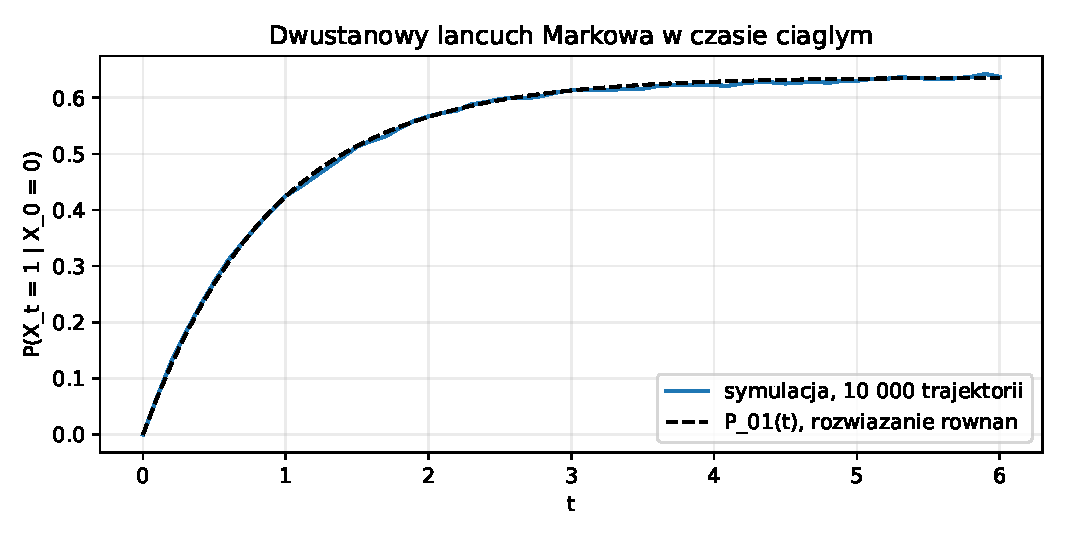
\includegraphics[width=0.88\textwidth]{figures/II_ctmc.pdf}\par
\small\emph{Rysunek: Równanie dwustanowego łańcucha a częstości z 10 000 trajektorii.}
\end{center}
\noindent\textbf{Kod w Pythonie (NumPy, Matplotlib).} Plik \texttt{code/II\_ctmc.py} można uruchomić niezależnie; zapisuje pokazany wykres.
\lstinputlisting[language=Python]{code/II_ctmc.py}
% --- KONIEC ROZSZERZENIA ILUSTRACYJNEGO ---

\section{Generatory, martyngały i wzór Dynkina}\label{sec:volII:05:08}
\begin{definicja}[Generator skończonego łańcucha]\label{def:volII:05:03}
Dla skończonego $E$, macierzy intensywności $Q$ i funkcji
$f:E\to\R$ definiujemy
\[
(Lf)(i):=\sum_{j\in E}q_{ij}f(j)
=\sum_{j\ne i}q_{ij}\bigl(f(j)-f(i)\bigr),\qquad i\in E.
\]
Operator $L$ na przestrzeni funkcji na $E$ nazywamy
generatorem procesu. W zapisie wektorowym $Lf=Qf$.
\end{definicja}

Druga postać wyjaśnia sens operatora: z każdego stanu $i$
ważymy zmiany wartości $f(j)-f(i)$ intensywnościami
bezpośrednich skoków. Dla funkcji stałej generator znika,
co jest analogią do pochodnej funkcji stałej.

\begin{twierdzenie}[Wzór Dynkina i martyngał generatorowy]\label{thm:volII:05:09}
\label{thm:dynkin}
Niech $E$ będzie skończone, $X$ łańcuchem w czasie
ciągłym o intensywnościach $Q$ i filtracji naturalnej.
Dla każdej funkcji $f:E\to\R$ proces
\[
M_t^f:=f(X_t)-f(X_0)-\int_0^t (Lf)(X_s)\,\dd s
\]
jest całkowalnym martyngałem.
W szczególności dla każdego $t\ge0$
\[
\E f(X_t)=\E f(X_0)+
\int_0^t\E[(Lf)(X_s)]\,\dd s.
\]
Jeśli $\tau$ jest ograniczonym czasem zatrzymania,
to również
\[
\E f(X_\tau)=\E f(X_0)+
\E\int_0^\tau (Lf)(X_s)\,\dd s.
\]
\end{twierdzenie}
\begin{proof}
Wszystkie funkcje na skończonym $E$ są ograniczone.
Z równania wstecznego, w zapisie operatorowym,
$\frac{\dd}{\dd t}P(t)f=P(t)Lf$.
Całkując od $0$ do $u$ dostajemy
$P(u)f-f=\int_0^u P(v)Lf\,\dd v$.
Dla $0\le s\le t$ własność Markowa implikuje
\[
\E[f(X_t)-f(X_s)\mid\calF_s]
=(P(t-s)f-f)(X_s).
\]
Jednocześnie $Lf$ jest funkcją ograniczoną na skończonym $E$, więc
$\int_s^t\E|Lf(X_u)|\,\dd u\le(t-s)\norm{Lf}_\infty<\infty$.
Dla każdego $A\in\calF_s$ możemy więc zastosować twierdzenie
Fubiniego do $\E[\ind A\int_s^t Lf(X_u)\,\dd u]$,
a następnie własność Markowa pod całką. Charakterystyka
warunkowej wartości oczekiwanej daje
\[
\E\left[\int_s^t(Lf)(X_u)\,\dd u\mid\calF_s\right]
=\int_0^{t-s}(P(v)Lf)(X_s)\,\dd v.
\]
Obie prawe strony są równe. Po odjęciu otrzymujemy
$\E[M_t^f-M_s^f\mid\calF_s]=0$.
Zatem $M^f$ jest martyngałem. Całkowalność jest
natychmiastowa, ponieważ $f$ i $Lf$ są ograniczone,
a rozważamy skończony czas $t$.

Biorąc wartości oczekiwane uzyskujemy pierwszą tożsamość.
Dla $\tau\le T$ twierdzenie o próbkowaniu opcjonalnym
z rozdziału 3 stosuje się do martyngału $M^f$, ponieważ
$\sup_{0\le t\le T}|M_t^f|\le2\norm f_\infty+T\norm{Lf}_\infty$.
Stąd $\E M_\tau^f=\E M_0^f=0$, co daje ostatni wzór.
\end{proof}

\begin{przyklad}[Przewidywana zmiana funkcji]
Dla modelu dwustanowego i $f(0)=0$, $f(1)=1$ mamy
$Lf(0)=\alpha$ i $Lf(1)=-\beta$.
Proces
\[
\ind{\{X_t=1\}}-\ind{\{X_0=1\}}
-\int_0^t\bigl(\alpha\ind{\{X_s=0\}}
-\beta\ind{\{X_s=1\}}\bigr)\,\dd s
\]
jest martyngałem. Człon podcałkowy opisuje
\emph{chwilową przewidywaną zmianę} wskaźnika awarii,
a jego odjęcie usuwa dryf.
\end{przyklad}

\section{Rozkłady stacjonarne, równowaga szczegółowa i ergodyczność}\label{sec:volII:05:09}
\begin{definicja}[Rozkład stacjonarny]\label{def:volII:05:04}
Dla łańcucha z $E$ skończonym i macierzą przejścia
$P(t)$ rozkład probabilistyczny $\pi=(\pi_i)_{i\in E}$
nazywamy \emph{stacjonarnym}, jeżeli
$\pi P(t)=\pi$ dla każdego $t\ge0$.
Rozkład $\pi$ spełnia \emph{równania bilansu} jeśli
$\pi Q=0$.
\end{definicja}

\begin{twierdzenie}[Bilans i równowaga szczegółowa]\label{thm:volII:05:10}
Niech $E$ będzie skończone i $Q$ macierzą intensywności.
Rozkład probabilistyczny $\pi$ jest stacjonarny wtedy i tylko
wtedy, gdy $\pi Q=0$. Warunkiem wystarczającym jest
\emph{równowaga szczegółowa}
\[
\pi_iq_{ij}=\pi_jq_{ji}\qquad\text{dla wszystkich }i,j\in E.
\]
\end{twierdzenie}
\begin{proof}
Jeśli $\pi P(t)=\pi$ dla każdego $t$, to przez różniczkowanie
w zerze otrzymujemy $\pi Q=0$.
Odwrotnie, gdy $\pi Q=0$, z rozwinięcia szeregu
$e^{tQ}=I+tQ+t^2Q^2/2!+\cdots$ wynika
$\pi e^{tQ}=\pi$, gdyż $\pi Q^k=0$ dla $k\ge1$.
Jeżeli zachodzi równowaga szczegółowa, to dla każdego $j$
\[
(\pi Q)_j=\sum_{i\ne j}\pi_iq_{ij}-\pi_j\sum_{k\ne j}q_{jk}
=\sum_{i\ne j}\pi_jq_{ji}-\pi_j\sum_{k\ne j}q_{jk}=0.
\]
Stąd $\pi Q=0$ i stacjonarność.
\end{proof}

Nie należy mylić bilansu całkowitego z równowagą szczegółową:
warunek szczegółowy jest silniejszy i nie zachodzi na przykład
dla jednokierunkowego ruchu po cyklu z co najmniej trzema
stanami, mimo istnienia rozkładu stacjonarnego.

\begin{twierdzenie}[Granica w modelu skończonym]\label{thm:volII:05:11}
Niech $E$ będzie skończonym zbiorem stanów, $Q$ macierzą
intensywności, a graf przejść z krawędzią $i\to j$ wtedy
i tylko wtedy, gdy $q_{ij}>0$, niech będzie silnie spójny.
Wtedy istnieje dokładnie jeden rozkład stacjonarny $\pi$;
wszystkie jego współrzędne są dodatnie i dla każdego
$i,j\in E$ zachodzi
$\lim_{t\to\infty}p_{ij}(t)=\pi_j$.
\end{twierdzenie}
\begin{proof}
Weźmy $\Lambda>\max_i q_i$ i $R=I+Q/\Lambda$.
Z silnej spójności grafu intensywności wynika
nieprzywiedlność dyskretnego łańcucha o macierzy $R$,
gdyż $R_{ij}>0$ dla $i\ne j$ dokładnie na dozwolonych
krawędziach. Ponieważ $R_{ii}>0$ dla każdego $i$,
łańcuch ten jest nieokresowy.
Twierdzenie o zbieżności skończonych nieprzywiedlnych
i nieokresowych łańcuchów z tomu I zapewnia istnienie
jedynego stacjonarnego $\pi$, dodatniego w każdym stanie,
i $R^n_{ij}\to\pi_j$ dla wszystkich $i,j$.
Warunek $\pi R=\pi$ jest równoważny $\pi Q=0$,
a więc rozkład jest też stacjonarny dla czasu ciągłego.

Z uniformizacji mamy
$p_{ij}(t)=\sum_{n\ge0}\Prob(N_t=n)R^n_{ij}$,
gdzie $N_t\sim\operatorname{Poisson}(\Lambda t)$.
Dla $\varepsilon>0$ wybierzmy $n_0$ tak, by
$|R^n_{ij}-\pi_j|<\varepsilon$ dla $n\ge n_0$.
Wtedy
\[
|p_{ij}(t)-\pi_j|
\le\Prob(N_t<n_0)+\varepsilon.
\]
Ponieważ $N_t\to\infty$ według prawdopodobieństwa
(gdy $t\to\infty$, choćby z nierówności Czebyszewa),
pierwszy składnik dąży do zera. Dajemy $\varepsilon\downarrow0$.
Jedyność rozkładu stacjonarnego wynika także z tego,
że każdy rozkład stacjonarny dla $Q$ jest stacjonarny dla $R$.
\end{proof}

\begin{przyklad}[Łańcuch trzystanowy na cyklu]
Niech $E=\{0,1,2\}$ i jedyne przejścia mają postać
$0\to1$, $1\to2$, $2\to0$, każde z intensywnością
$\lambda>0$. Wtedy
\[
Q=\lambda\begin{pmatrix}-1&1&0\\0&-1&1\\1&0&-1\end{pmatrix}.
\]
Rozkład $\pi=(1/3,1/3,1/3)$ spełnia $\pi Q=0$,
więc jest stacjonarny. Graf jest silnie spójny,
zatem proces zbiega rozkładem do $\pi$.
Jednak równowaga szczegółowa nie zachodzi, bo
$\pi_0q_{01}=\lambda/3>0$ i $\pi_1q_{10}=0$.
Proces ma więc stacjonarny, niezerowy przepływ wokół cyklu.
\end{przyklad}

\section{Łańcuchy urodzin i śmierci}\label{sec:volII:05:10}
\begin{definicja}[Proces urodzin i śmierci]\label{def:volII:05:05}
Niech $E=\N_0$. Procesem urodzin i śmierci nazywamy
minimalny łańcuch Markowa o jedynych dozwolonych przejściach
$n\to n+1$ z intensywnością $\lambda_n\ge0$ i
$n\to n-1$ z intensywnością $\mu_n\ge0$ dla $n\ge1$,
przy $\mu_0:=0$. Pozostałe wyrazy pozadiagonalne są zerowe,
a $q_{nn}=-(\lambda_n+\mu_n)$.
\end{definicja}

Nazwa nawiązuje do populacji, w której każda zmiana liczebności
jest zwiększeniem lub zmniejszeniem o jeden. Ta sama
matematyka opisuje jednak liczbę klientów w kolejce, cząstek
w systemie czy liczebność aktywnych urządzeń.

\begin{stwierdzenie}[Rozkład stacjonarny przy równowadze lokalnej]\label{prop:volII:05:01}
Załóżmy, że $\lambda_n>0$ dla $n\ge0$,
$\mu_n>0$ dla $n\ge1$, oraz że proces jest nieeksplodujący.
Jeżeli
\[
Z:=1+\sum_{n=1}^\infty
\prod_{k=0}^{n-1}\frac{\lambda_k}{\mu_{k+1}}<\infty,
\]
to liczby
$\pi_0:=1/Z$ i
$\pi_n:=Z^{-1}\prod_{k=0}^{n-1}\lambda_k/\mu_{k+1}$
dla $n\ge1$ tworzą rozkład probabilistyczny spełniający
równowagę szczegółową
$\pi_n\lambda_n=\pi_{n+1}\mu_{n+1}$.
W szczególności $\pi$ jest rozkładem stacjonarnym procesu.
\end{stwierdzenie}
\begin{proof}
Wszystkie $\pi_n$ są nieujemne, a ich suma z definicji
jest równa $Z/Z=1$. Przez skrócenie kolejnych iloczynów
otrzymujemy $\pi_n\lambda_n=\pi_{n+1}\mu_{n+1}$.
Wykazaliśmy zatem równowagę szczegółową.
Pozostaje udowodnić stacjonarność \emph{dla procesu
nieskończeniewymiarowego}; nie wystarczy tylko zapisać
formalnej równości $\pi Q=0$.

Dla $K\in\N$ rozważmy łańcuch na $\{0,1,\ldots,K\}$
z tymi samymi intensywnościami, z wyjątkiem tego,
że tłumimy przejście $K\to K+1$.
Jest to skończony, nieeksplodujący proces,
a jego rozkład
\[
\pi_n^{(K)}:=\frac{\pi_n}{\sum_{k=0}^K\pi_k},
\qquad 0\le n\le K,
\]
spełnia równowagę szczegółową dla wszystkich jego krawędzi,
a więc jest stacjonarny w myśl twierdzenia skończonego.

Dla ustalonego stanu początkowego $i\in\N_0$ skonstruujmy
proces obcięty i pierwotny przy użyciu \emph{tych samych}
losowań skoków i czasów przebywania, aż do pierwszej próby
wyjścia poza $\{0,\ldots,K\}$. Do tej chwili oba procesy
są jednakowe. Ponieważ oryginalny proces jest nieeksplodujący,
na każdym $[0,t]$ wykonuje tylko skończenie wiele skoków
prawie na pewno; jego trajektoria ma zatem na $[0,t]$
skończone maksimum. Stąd dla każdego $i,j$ i $t$
\[
P_t^{(K)}(i,j)\longrightarrow P_t(i,j)
\quad (K\to\infty,\ K\ge i),
\]
gdzie $P_t^{(K)}$ oznacza macierz przejścia łańcucha
obciętego.

Teraz ustalmy $j$ i $t$. Stacjonarność $\pi^{(K)}$ daje
\[
\pi_j^{(K)}=\sum_{i=0}^K\pi_i^{(K)}P_t^{(K)}(i,j).
\]
Dla ustalonego $i$ mamy $\pi_i^{(K)}\to\pi_i$
i zbieżność odpowiednich prawdopodobieństw przejścia.
Ponieważ $\sum_{i\ge0}\pi_i=1$, ogon
$\sum_{i>M}\pi_i$ jest dowolnie mały, a dla dużych $K$
$\pi_i^{(K)}\le2\pi_i$. Stąd możemy najpierw przepuścić
$K\to\infty$ w skończonej sumie po $i\le M$,
a następnie $M\to\infty$ kontrolując ogon przez
$2\sum_{i>M}\pi_i$. Otrzymujemy
$\pi_j=\sum_{i\ge0}\pi_iP_t(i,j)$.
Ponieważ $j,t$ były dowolne, $\pi$ jest stacjonarna.
\end{proof}

\begin{uwaga}[Wersja nieskończona wymaga ostrożności]
W poprzednim stwierdzeniu założyliśmy nieeksplodowanie.
W ogólnych modelach na przestrzeni przeliczalnej
formalna równość $\pi Q=0$ nie jest automatycznie
równoważna stacjonarności minimalnego procesu,
gdy masa może uciekać przez eksplozję. Z tego powodu
nie przenosimy bez komentarza wyników z przypadku
skończonego na wszystkie macierze $Q$.
\end{uwaga}


\begin{uwaga}[Dlaczego obcięcie nieskończonego łańcucha wymaga sprzężenia?]
W dowodzie stacjonarności procesu urodzin i śmierci
przybliżamy łańcuch na $\N_0$ przez łańcuchy na
$\{0,\ldots,K\}$. Nie wystarczy tylko stwierdzić, że
macierze intensywności są podobne: w stanie brzegowym $K$
mają inne czasy przebywania. Można jednak \emph{sprzęgnąć}
procesy, korzystając z tych samych niezależnych zegarów
potencjalnych przejść $n\to n+1$ i $n\to n-1$.
W łańcuchu obciętym ignorujemy wyłącznie impulsy
$K\to K+1$; pozostałe są wspólne dla obu procesów.
Do pierwszego wejścia oryginalnego procesu w $K+1$
trajektorie obu procesów są więc identyczne.
Przy założonym braku eksplozji liczba skoków procesu
oryginalnego na $[0,t]$ jest prawie na pewno skończona,
co oznacza, że na tym przedziale osiąga tylko skończenie
wiele stanów. Dla każdego ustalonego wyniku losowania
oraz dostatecznie dużego $K$ przybliżenia i oryginał
zgadzają się na całym $[0,t]$.
To uzasadnia zbieżność ich praw przejścia, a dopiero
następnie można przejść do granicy w równaniu stacjonarności.
\end{uwaga}

\begin{uwaga}[Zanik pamięci a własność Markowa]
Własność Markowa mówi, że po znajomości $X_t$ cała
wcześniejsza historia nie jest potrzebna do prognozowania
przyszłości. Nie oznacza, że rozkład $X_t$ przestaje
zależeć od stanu początkowego w krótkim czasie.
Asymptotyczny zanik tej zależności wynika w modelu
skończonym z nieprzywiedlności i twierdzenia o granicy
$P(t)$; dla niektórych procesów na przestrzeniach
nieskończonych taki wynik może być fałszywy.
\end{uwaga}

\section{Model kolejki \texorpdfstring{$M/M/1$}{M/M/1}}\label{sec:volII:05:11}
\begin{przyklad}[Pojedynczy serwer]
Klienci napływają zgodnie z procesem Poissona o intensywności
$\lambda>0$. Czasy obsługi są niezależne, mają rozkład
$\operatorname{Exp}(\mu)$ z $\mu>0$ i są niezależne
od napływu. Jeden serwer obsługuje co najwyżej jednego klienta
naraz, a klienci czekają bez ograniczenia pojemności.
Stanem $X_t$ jest liczba osób w systemie (obsługiwanych
i oczekujących). Przy $X_t=n$ nowy klient zwiększa stan do
$n+1$ z intensywnością $\lambda$, a przy $n\ge1$
zakończenie obsługi zmniejsza stan do $n-1$ z intensywnością
$\mu$. Jest to proces urodzin i śmierci z
$\lambda_n=\lambda$ i $\mu_n=\mu$ dla $n\ge1$.

Z poprzedniego stwierdzenia otrzymujemy dla
$\rho:=\lambda/\mu<1$:
\[
\pi_n=(1-\rho)\rho^n,\qquad n\in\N_0.
\]
Sprawdźmy też, dlaczego $\rho<1$ jest konieczne dla
istnienia rozkładu stacjonarnego. Każdy taki rozkład
spełnia równanie bilansu w stanie $0$:
$\lambda\pi_0=\mu\pi_1$.
Bilans w stanie $n\ge1$ brzmi
$\lambda\pi_{n-1}+\mu\pi_{n+1}=(\lambda+\mu)\pi_n$.
Indukcyjnie wynika stąd $\pi_{n+1}=\rho\pi_n$, gdyż
równość dla $n=0$ jest początkiem indukcji, a podstawienie
$\lambda\pi_{n-1}=\mu\pi_n$ do równania dla $n$
prowadzi do $\mu\pi_{n+1}=\lambda\pi_n$.
Stąd $\pi_n=\rho^n\pi_0$, a możliwość normalizacji wymaga
$\rho<1$. Wtedy $\pi_0=1-\rho$.
W tym stanie równowagi
$\Prob(X_t=0)=1-\rho$ i
$\E X_t=\sum_{n\ge0}n(1-\rho)\rho^n=\rho/(1-\rho)$.
Ostatni wzór otrzymujemy różniczkując szereg geometryczny
$\sum_{n\ge0}\rho^n=(1-\rho)^{-1}$ dla $0<\rho<1$.

Brak eksplozji wynika z faktu, że całkowita intensywność
jest ograniczona przez $\lambda+\mu$. Przy $\rho\ge1$
proces nadal istnieje, lecz nie ma rozkładu stacjonarnego
normalizowalnego na $\N_0$.
\end{przyklad}

\begin{zadanie}[Kolejka i liczba klientów]
Do stanowiska przychodzi średnio $3$ klientów na godzinę,
a jeden serwer obsługuje średnio $5$ klientów na godzinę;
napływ i czasy obsługi spełniają założenia modelu $M/M/1$.
Obliczyć w stanie stacjonarnym: (a) prawdopodobieństwo
pustego systemu; (b) prawdopodobieństwo obecności co
najmniej trzech klientów; (c) średnią liczbę klientów.

\emph{Rozwiązanie.} Mamy $\rho=3/5$. Zatem
$\pi_0=1-\rho=2/5$.
Dalej
$\Prob(X\ge3)=\sum_{n=3}^\infty(1-\rho)\rho^n
=\rho^3=27/125$.
Średnia wynosi $\rho/(1-\rho)=\frac{3/5}{2/5}=3/2$.
Wszystkie te wyniki dotyczą \emph{stanu stacjonarnego};
nie są poprawnymi odpowiedziami na pytania o układ,
który właśnie został uruchomiony z zerową liczbą klientów.
\end{zadanie}

\section{Model Ehrenfesta w czasie ciągłym}\label{sec:volII:05:12}
\begin{przyklad}[Dwie komory]
Niech $K\in\N$ cząstek niezależnie przemieszcza się
między komorami $A$ i $B$. Każda cząstka w $B$ przechodzi
do $A$ z intensywnością $\alpha>0$, a każda cząstka w $A$
przechodzi do $B$ z intensywnością $\beta>0$.
Niech $X_t$ oznacza liczbę cząstek w $A$ w chwili $t$.
Gdy $X_t=i$, w $B$ znajduje się $K-i$ cząstek, więc
$\lambda_i=(K-i)\alpha$, a $\mu_i=i\beta$.
Łańcuch na $\{0,\ldots,K\}$ jest nieprzywiedlny.

Dla $p:=\alpha/(\alpha+\beta)$ rozkład
\[
\pi_i=\binom Ki p^i(1-p)^{K-i},\qquad 0\le i\le K,
\]
jest stacjonarny. Rzeczywiście,
\begin{align*}
\frac{\pi_{i+1}}{\pi_i}
&=\frac{K-i}{i+1}\frac{p}{1-p}
=\frac{(K-i)\alpha}{(i+1)\beta}
=\frac{\lambda_i}{\mu_{i+1}},
\end{align*}
co dokładnie oznacza równowagę szczegółową
$\pi_i\lambda_i=\pi_{i+1}\mu_{i+1}$.
Rozkład dwumianowy pojawia się zatem nie tylko
przy niezależnych próbach, lecz także jako prawo
stacjonarne łańcucha w czasie ciągłym.
\end{przyklad}

\section{Czas pochłonięcia i macierz fundamentalna}\label{sec:volII:05:13}
\begin{twierdzenie}[Oczekiwany czas pochłonięcia]\label{thm:volII:05:12}
\label{thm:ctmc-absorption}
Niech $E=T\mathbin{\dot\cup}A$ będzie skończonym zbiorem stanów,
$A\ne\varnothing$ zbiorem stanów pochłaniających,
a $T$ zbiorem stanów niepochłaniających. Przy uporządkowaniu
najpierw stanów $T$ macierz intensywności ma blokową postać
\[
Q=\begin{pmatrix}B&C\\0&0\end{pmatrix}.
\]
Załóżmy, że startując z każdego $i\in T$, proces
osiąga $A$ z prawdopodobieństwem jeden.
Wtedy $B$ jest odwracalna, macierz
$G:=(-B)^{-1}$ ma nieujemne wyrazy i
\[
G_{ij}=\E_i\left[\int_0^\tau\ind{\{X_t=j\}}\,\dd t\right],
\qquad
\E_i\tau=\sum_{j\in T}G_{ij},
\]
gdzie $\tau=\inf\{t\ge0:X_t\in A\}$, a
$\E_i$ oznacza wartość oczekiwaną dla procesu
startującego ze stanu $i$.
\end{twierdzenie}
\begin{proof}
Stany z $A$ są pochłaniające, dlatego dla $i,j\in T$
$\Prob_i(X_t=j,\tau>t)=\Prob_i(X_t=j)$.
Macierz przejścia ograniczona do $T$ jest równa $e^{tB}$:
wynika to z blokowo-trójkątnej postaci $e^{tQ}$,
którą widać bezpośrednio z potęg macierzy $Q$.
Stąd całkując funkcję wskaźnikową i stosując Tonellego,
\[
\E_i\int_0^\tau\ind{\{X_t=j\}}\,\dd t
=\int_0^\infty\Prob_i(X_t=j,\tau>t)\,\dd t
=\int_0^\infty(e^{tB})_{ij}\,\dd t.
\]

Musimy wykazać zbieżność tej całki oraz odwracalność $B$.
Ponieważ proces z każdego stanu $i\in T$ zostaje pochłonięty
prawie na pewno, istnieje $t_i>0$ takie, że
$\Prob_i(\tau>t_i)<1/2$. Biorąc $t_0=\max_i t_i$,
z monotoniczności funkcji przeżycia dostajemy
$\sup_{i\in T}\Prob_i(\tau>t_0)\le1/2$.
Własność Markowa w chwilach $nt_0$ pokazuje indukcyjnie,
że $\sup_i\Prob_i(\tau>nt_0)\le2^{-n}$.
Zatem wierszowe sumy macierzy $e^{tB}$ maleją
wykładniczo do zera, a nieujemne wyrazy tej macierzy
są całkowalne na $[0,\infty)$. Niech
$G=\int_0^\infty e^{tB}\,\dd t$.
Z równania $\frac{\dd}{\dd t}e^{tB}=Be^{tB}$ wynika
\[
BG=\lim_{t\to\infty}e^{tB}-I=-I.
\]
W skończonym wymiarze istnienie prawej odwrotności
macierzy kwadratowej oznacza odwracalność, a
$G=(-B)^{-1}$. Nieujemność wyrazów jest widoczna
z całkowej reprezentacji. Sumując tożsamość
$\int_0^\tau\sum_{j\in T}\ind{\{X_t=j\}}\,\dd t=\tau$
(na $[0,\tau)$ proces pozostaje w $T$)
po $j$ i biorąc wartości oczekiwane,
otrzymujemy drugi wzór.
\end{proof}

\begin{zadanie}[Pełne obliczenie czasu pochłonięcia]
Rozważmy łańcuch z trzema stanami i intensywnościami
$0\to1$ z intensywnością $2$, $1\to0$ z intensywnością $1$
oraz $1\to2$ z intensywnością $3$.
Stan $2$ jest pochłaniający. Obliczyć oczekiwany czas
osiągnięcia stanu $2$ przy starcie ze stanu $0$ i $1$,
a także oczekiwany łączny czas spędzony w stanach $0$ i $1$
przed pochłonięciem przy starcie z $0$.

\emph{Rozwiązanie.} Macierz intensywności jest równa
\[
Q=\begin{pmatrix}-2&2&0\\1&-4&3\\0&0&0\end{pmatrix},
\quad
B=\begin{pmatrix}-2&2\\1&-4\end{pmatrix}.
\]
Pochłonięcie zachodzi prawie na pewno: przy każdym wejściu
do stanu $1$ następny skok prowadzi do $2$ z
prawdopodobieństwem $3/4$, a powroty do stanu $1$ po skoku
do $0$ następują prawie na pewno. Prawdopodobieństwo
uniknięcia stanu $2$ po $m$ wizytach w $1$ wynosi $(1/4)^m$,
co dąży do zera.
Z twierdzenia~\ref{thm:ctmc-absorption}
\[
G=(-B)^{-1}
=\begin{pmatrix}2&-2\\-1&4\end{pmatrix}^{-1}
=\frac16\begin{pmatrix}4&2\\1&2\end{pmatrix}.
\]
Przy starcie z $0$ oczekiwane czasy zajmowania kolejno
stanu $0$ i stanu $1$ wynoszą $4/6=2/3$ oraz $2/6=1/3$.
Ich suma to $\E_0\tau=1$. Przy starcie z $1$ suma
elementów drugiego wiersza daje $\E_1\tau=1/2$.

\emph{Sprawdzenie bez macierzy.} Oznaczmy
$u_i=\E_i\tau$, $u_2=0$.
Ze stanu $0$ oczekujemy średnio $1/2$ jednostki czasu
i przechodzimy do $1$, więc $u_0=1/2+u_1$.
Ze stanu $1$ czekamy średnio $1/4$, po czym z
prawdopodobieństwem $1/4$ przechodzimy do $0$,
a z $3/4$ do $2$. Stąd
$u_1=1/4+(1/4)u_0$. Rozwiązanie daje
$u_0=1$, $u_1=1/2$ zgodnie z rachunkiem macierzowym.
To jest praktyczna metoda \emph{analizy pierwszego skoku}.
\end{zadanie}

\section{Jak czytać prawdopodobieństwa trajektorii?}\label{sec:volII:05:14}
Przy procesie dyskretnym używaliśmy wzoru
$\Prob(X_0=i_0,\ldots,X_n=i_n)$.
W czasie ciągłym należy rozróżnić obserwacje
w \emph{ustalonych chwilach} od zarejestrowania
\emph{dokładnych czasów skoków}.

\begin{stwierdzenie}[Wspólny rozkład obserwacji w ustalonych chwilach]\label{prop:volII:05:02}
Niech $X$ będzie skończonym łańcuchem w czasie ciągłym,
$0=t_0<t_1<\cdots<t_n$, a $\mu$ rozkładem początkowym.
Wtedy dla każdego $i_0,\ldots,i_n\in E$
\[
\Prob(X_{t_0}=i_0,\ldots,X_{t_n}=i_n)
=\mu_{i_0}\prod_{k=1}^n
 p_{i_{k-1},i_k}(t_k-t_{k-1}).
\]
\end{stwierdzenie}
\begin{proof}
Jeżeli prawdopodobieństwo wcześniejszej części zdarzenia
jest dodatnie, stosujemy łańcuchowy wzór na prawdopodobieństwo
warunkowe. Własność Markowa daje
\[
\Prob(X_{t_k}=i_k\mid X_{t_0}=i_0,\ldots,X_{t_{k-1}}=i_{k-1})
=p_{i_{k-1},i_k}(t_k-t_{k-1}).
\]
Mnożymy kolejne czynniki, rozpoczynając od
$\Prob(X_{t_0}=i_0)=\mu_{i_0}$.
Jeżeli prawdopodobieństwo wcześniejszego zdarzenia jest zero,
to prawdopodobieństwo całej ścieżki obserwacji również
jest zero, a iloczyn po prawej zawiera zerowy czynnik
na pierwszym etapie, na którym otrzymujemy zerowy iloczyn.
W ten sposób wzór obejmuje także zdarzenia zerowe.
\end{proof}

\begin{uwaga}[Prawdopodobieństwo dokładnej chwili skoku]
Jeżeli $J_1$ jest pierwszą chwilą skoku ze stanu $i$ o
$q_i>0$, to $J_1\sim\operatorname{Exp}(q_i)$ i
$\Prob(J_1=t)=0$ dla każdego ustalonego $t\ge0$.
Nie pytamy więc o \emph{prawdopodobieństwo} dokładnego czasu,
lecz o jego \emph{gęstość}. Dla ściśle rosnących
$0<s_1<\cdots<s_m<t$ oraz ciągu rzeczywistych zmian
$i_0\to i_1\to\cdots\to i_m$ gęstość zdarzenia:
``skoki nastąpiły w chwilach $s_1,\ldots,s_m$,
a do $t$ nie nastąpił następny skok'' jest równa
\[
\mu_{i_0}\left[\prod_{k=1}^m
q_{i_{k-1},i_k}e^{-q_{i_{k-1}}(s_k-s_{k-1})}\right]
e^{-q_{i_m}(t-s_m)},\qquad s_0:=0.
\]
Wynika to z mnożenia gęstości wykładniczych czasów
przebywania i prawdopodobieństw wyboru kolejnych stanów:
$[q_i e^{-q_i u}](q_{ij}/q_i)=q_{ij}e^{-q_i u}$.
To zapis, od którego zaczyna się matematyczne formułowanie
wiarygodności ciągłych trajektorii procesów skokowych;
sama statystyczna estymacja należy jednak do tomu III.
\end{uwaga}

\section{Podsumowanie i połączenie z procesem Wienera}\label{sec:volII:05:15}
Proces Poissona miał \emph{stałą} intensywność skoków,
a jego stan zawsze wzrastał o jeden. Łańcuch w czasie
ciągłym dopuszcza zależną od stanu intensywność $q_i$,
różne kierunki zmian oraz pochłanianie. Procesy te nadal
mają trajektorie schodkowe.

W następnych rozdziałach zajmiemy się procesami gaussowskimi
i procesem Wienera, których ciągłe trajektorie różnią się
zasadniczo od trajektorii Poissona. Pomimo tej różnicy
oba światy połączą wspólne narzędzia: filtracje, martyngały,
generatory i równania Kołmogorowa. Jeszcze później
zbudujemy całkę stochastyczną i miarę Wienera na przestrzeni
trajektorii, a następnie zbadamy jej związek z całkami
funkcyjnymi w mechanice kwantowej.


% ==============================================================
% TOM II — ROZDZIAŁ 6: PROCESY GAUSSOWSKIE
% ==============================================================
\chapter{Procesy gaussowskie: od kowariancji do prawa procesu}
\label{chap:volII:06}
\par\smallskip\noindent{\small\textit{Powiązania:} \textup{tom~I}, sekcja~\ref{I-sec:volI:04:04} (wektory losowe); sekcja~\ref{sec:volII:07:01} (proces Wienera); \textup{tom~III}, sekcja~\ref{III-sec:volIII:09:03} (przestrzeń Camerona–Martina); twierdzenie~\ref{thm:volII:02:02} (kryterium ciągłości Kołmogorowa).}\par\smallskip

\label{ch:gauss}

\section{Motywacja: czy średnia i kowariancja opisują cały proces?}\label{sec:volII:06:01}
W rozdziale pierwszym zobaczyliśmy, że znajomość rozkładu $X_t$ dla
każdego $t$ nie wystarcza do określenia prawa procesu: potrzebujemy
rozkładów \emph{łącznych} dla wszystkich skończonych zbiorów chwil.
W ogólności obliczanie tych rozkładów jest bardzo trudne. Procesy
gaussowskie są niezwykłe właśnie dlatego, że wszystkie ich rozkłady
skończeniewymiarowe można odtworzyć z dwóch funkcji:
$m(t)=\E X_t$ oraz $K(s,t)=\Cov(X_s,X_t)$.

Warto od razu oddzielić \emph{gaussowskość pojedynczych zmiennych}
od \emph{gaussowskości całego procesu}. Można mieć $X_s\sim\Normal(0,1)$
i $X_t\sim\Normal(0,1)$, choć para $(X_s,X_t)$ nie ma rozkładu
normalnego dwuwymiarowego. Dopiero odpowiedni warunek na każdą
skończoną rodzinę rozstrzyga o gaussowskości procesu.

\begin{definicja}[Wektor gaussowski]\label{def:volII:06:01}
Niech $d\in\N$ i $Z=(Z_1,\ldots,Z_d)$ będzie wektorem losowym
o wartościach w $\R^d$. Nazywamy go \emph{wektorem gaussowskim},
jeżeli dla każdego $a\in\R^d$ zmienna $\sum_{j=1}^d a_jZ_j$
ma rozkład normalny (dopuszczamy rozkład zdegenerowany, czyli
skoncentrowany w jednym punkcie). Jeżeli $m=\E Z$ oraz
$\Sigma=(\Cov(Z_i,Z_j))_{i,j=1}^d$, zapisujemy
$Z\sim\Normal_d(m,\Sigma)$.
\end{definicja}

Dopuszczenie degeneracji nie jest tylko wygodą techniczną. Dla
$Z=(U,U)$, gdzie $U\sim\Normal(0,1)$, wektor $Z$ jest gaussowski,
ale jego rozkład jest skoncentrowany na przekątnej $\{(x,x):x\in\R\}$,
więc nie ma gęstości względem dwuwymiarowej miary Lebesgue'a.

\begin{stwierdzenie}[Charakterystyka wektora gaussowskiego]\label{prop:volII:06:01}
Dla każdego $d\ge1$, $m\in\R^d$ i symetrycznej nieujemnie
określonej macierzy $\Sigma\in\R^{d\times d}$ istnieje wektor
$Z\sim\Normal_d(m,\Sigma)$, którego funkcja charakterystyczna ma postać
\[
\E e^{i\langle u,Z\rangle}
=\exp\left(i\langle u,m\rangle-\frac12 u^\top\Sigma u\right),
\qquad u\in\R^d.
\]
Prawo tego wektora jest jednoznacznie wyznaczone przez $m$ i $\Sigma$.
\end{stwierdzenie}
\begin{proof}
Z twierdzenia spektralnego mamy $\Sigma=ADA^\top$, gdzie $A$
jest ortogonalna, $D=\operatorname{diag}(\lambda_1,\ldots,\lambda_d)$
i $\lambda_j\ge0$. Niech $G_1,\ldots,G_d$ będą niezależnymi
zmiennymi $\Normal(0,1)$ i połóżmy
$Z=m+AD^{1/2}G$. Wówczas
$\langle u,Z-m\rangle$ jest liniową kombinacją niezależnych
zmiennych normalnych, a zatem jest normalna o wariancji
$u^\top AD A^\top u=u^\top\Sigma u$. Jego funkcję charakterystyczną
otrzymujemy, mnożąc funkcje charakterystyczne składników.
Z jednoznaczności funkcji charakterystycznej wynika jednoznaczność
rozkładu wektora $Z$.
\end{proof}

\begin{definicja}[Proces gaussowski]\label{def:volII:06:02}
Niech $T\ne\varnothing$ będzie zbiorem indeksów oraz
$(\Omega,\calF,\Prob)$ przestrzenią probabilistyczną. Proces
rzeczywisty $(X_t)_{t\in T}$ na tej przestrzeni nazywamy
\emph{gaussowskim}, jeżeli dla dowolnego $n\ge1$ oraz
$t_1,\ldots,t_n\in T$ wektor $(X_{t_1},\ldots,X_{t_n})$
jest gaussowski. Definiujemy
$m(t):=\E X_t$ i $K(s,t):=\E[(X_s-m(s))(X_t-m(t))]$.
\end{definicja}

\begin{twierdzenie}[Średnia i kowariancja wyznaczają prawo]\label{thm:volII:06:01}
Niech $X=(X_t)_{t\in T}$ i $Y=(Y_t)_{t\in T}$ będą rzeczywistymi
procesami gaussowskimi (niekoniecznie na tej samej przestrzeni).
Jeżeli dla wszystkich $s,t\in T$ zachodzą równości
$\E X_t=\E Y_t$ i $\Cov(X_s,X_t)=\Cov(Y_s,Y_t)$, to $X$ i $Y$
mają te same rozkłady skończeniewymiarowe.
\end{twierdzenie}
\begin{proof}
Ustalmy $t_1,\ldots,t_n$. Oba odpowiadające im wektory są
gaussowskie, mają wektor średnich
$(m(t_1),\ldots,m(t_n))$ i tę samą macierz kowariancji
$(K(t_i,t_j))_{i,j}$. Z poprzedniego stwierdzenia ich funkcje
charakterystyczne są identyczne. Jednoznaczność funkcji
charakterystycznej daje równość rozkładów. Ponieważ wybór chwil był
dowolny, otrzymujemy tezę.
\end{proof}

\begin{uwaga}[Dlaczego warunek wspólnej normalności jest istotny?]
Niech $U\sim\Normal(0,1)$, a $\varepsilon$ będzie od niego
niezależnym symetrycznym znakiem o wartościach $\pm1$.
Wtedy $X=U$, $Y=\varepsilon U$ mają standardowe rozkłady normalne,
a $\Cov(X,Y)=0$, ponieważ $\E\varepsilon=0$.
Jednak $|X|=|Y|$ prawie na pewno, zatem zmienne są zależne,
a para $(X,Y)$ nie jest wektorem gaussowskim.
Wektor gaussowski o takiej macierzy kowariancji miałby niezależne
współrzędne, co jest sprzeczne z $|X|=|Y|$.
\end{uwaga}

\section{Jakie funkcje mogą być kowariancjami?}\label{sec:volII:06:02}
Zachodzi $K(s,t)=K(t,s)$, ale sama symetria nie wystarcza.
Dla dowolnych $t_1,\ldots,t_n\in T$ i $a_1,\ldots,a_n\in\R$
mamy
\[
\sum_{i,j=1}^n a_i a_jK(t_i,t_j)
=\Var\left(\sum_{i=1}^n a_iX_{t_i}\right)\ge0.
\]
Warunek ten nazywamy \emph{nieujemną określonością jądra} $K$.

\begin{twierdzenie}[Istnienie procesu o zadanej kowariancji]\label{thm:volII:06:02}
Niech $T\ne\varnothing$ będzie dowolnym zbiorem,
$m:T\to\R$ dowolną funkcją, zaś $K:T\times T\to\R$
niech spełnia warunki: $K(s,t)=K(t,s)$ oraz
$\sum_{i,j=1}^n a_i a_jK(t_i,t_j)\ge0$ dla wszystkich
$n\in\N$, $t_1,\ldots,t_n\in T$ i $a_1,\ldots,a_n\in\R$.
Wtedy istnieje przestrzeń probabilistyczna i rzeczywisty proces
gaussowski $X=(X_t)_{t\in T}$, dla którego
$\E X_t=m(t)$ oraz $\Cov(X_s,X_t)=K(s,t)$.
\end{twierdzenie}
\begin{proof}
Dla każdej skończonej uporządkowanej rodziny chwil
$\mathbf t=(t_1,\ldots,t_n)$ wybierzmy rozkład gaussowski
$\mu_{\mathbf t}=\Normal_n(m_{\mathbf t},\Sigma_{\mathbf t})$,
gdzie $m_{\mathbf t}=(m(t_1),\ldots,m(t_n))$,
$\Sigma_{\mathbf t}=(K(t_i,t_j))_{i,j}$. Jest to dobrze określony
rozkład, bo macierz kowariancji jest nieujemnie określona.

Trzeba sprawdzić zgodność tej rodziny. Usunięcie części współrzędnych
z wektora gaussowskiego daje wektor gaussowski, którego średnia i
kowariancja są odpowiednimi podwektorami i podmacierzami.
Zmiana kolejności współrzędnych jedynie permutuje średnią i macierz.
Przy powtórzeniu chwili $t_i=t_j$ różnica odpowiednich współrzędnych
ma wariancję $K(t_i,t_i)+K(t_j,t_j)-2K(t_i,t_j)=0$ i średnią zero;
zatem współrzędne są równe prawie na pewno.
Warunki zgodności obowiązują więc także dla powtórzonych chwil.

Możemy teraz zastosować udowodnione w rozdziale~\ref{ch:konstrukcja}
twierdzenie Kołmogorowa o istnieniu procesu, które daje proces
z zadanymi rozkładami skończeniewymiarowymi. Wszystkie te rozkłady
są gaussowskie, a ich średnie i kowariancje są równe $m,K$.
\end{proof}

\begin{przyklad}[Losowa prosta i losowa fala]
Niech $A,B$ będą niezależne o rozkładzie $\Normal(0,1)$.
Proces $X_t=A+tB$ ma średnią zero i kowariancję
$K_X(s,t)=1+st$. Jego trajektorie są prostymi; proces jest
gaussowski, ponieważ każda skończona rodzina jego wartości
jest liniowym obrazem wektora $(A,B)$.

Dla ustalonej $\omega_0>0$ proces
$Y_t=A\cos(\omega_0t)+B\sin(\omega_0t)$ również jest gaussowski,
a $K_Y(s,t)=\cos(\omega_0(t-s))$. Jest to proces stacjonarny
w sensie rozkładów skończeniewymiarowych, choć każda trajektoria
jest gładką, okresową funkcją. Stacjonarność nie wymaga więc
ani niezależnych wartości, ani nieregularnych trajektorii.
\end{przyklad}

\begin{przyklad}[Kowariancja wykładnicza: proces typu Ornsteina--Uhlenbecka]
Ustalmy $\sigma>0$ i $\alpha>0$. Zdefiniujmy
$K(s,t)=\sigma^2 e^{-\alpha|t-s|}$ dla $s,t\ge0$.
Rzeczywiście jest to jądro nieujemnie określone, ponieważ
\[
K(s,t)=2\alpha\sigma^2\int_{-\infty}^{\min(s,t)}
 e^{-\alpha(s-u)}e^{-\alpha(t-u)}\,\dd u.
\]
Dla dowolnych $a_i,t_i$ odpowiadająca mu forma kwadratowa jest
całką z nieujemnego kwadratu:
\[
\sum_{i,j}a_ia_jK(t_i,t_j)=2\alpha\sigma^2\int_{-\infty}^\infty
\left(\sum_i a_i\ind{\{u\le t_i\}}e^{-\alpha(t_i-u)}\right)^2\dd u\ge0.
\]
Poprzednie twierdzenie daje zatem stacjonarny proces gaussowski
$Y$ o tej kowariancji. Co więcej,
$\E|Y_t-Y_s|^4=3\,[2\sigma^2(1-e^{-\alpha|t-s|})]^2
\le12\sigma^4\alpha^2|t-s|^2$.
Kryterium ciągłości Kołmogorowa zapewnia istnienie jego ciągłej
modyfikacji. Nie użyliśmy przy tym całki Itô, którą zdefiniujemy
dopiero w dalszych rozdziałach.
\end{przyklad}

\section{Niezależność i warunkowanie dla procesów gaussowskich}\label{sec:volII:06:03}
\begin{twierdzenie}[Nieskorelowane podwektory gaussowskie są niezależne]\label{thm:volII:06:03}
Niech $(U,V)$ będzie wektorem gaussowskim o wartościach
w $\R^k\times\R^m$. Jeżeli $\Cov(U_i,V_j)=0$
dla wszystkich $i,j$, to wektory $U$ i $V$ są niezależne.
\end{twierdzenie}
\begin{proof}
Macierz kowariancji wektora $(U,V)$ jest blokowo diagonalna:
$\Sigma=\operatorname{diag}(\Sigma_U,\Sigma_V)$.
Jego funkcja charakterystyczna w punkcie $(u,v)$ jest zatem
iloczynem funkcji charakterystycznych $U$ i $V$,
ponieważ wyrażenie kwadratowe rozdziela się na sumę
$u^\top\Sigma_Uu+v^\top\Sigma_Vv$.
Z jednoznaczności funkcji charakterystycznych wnioskujemy,
że rozkład $(U,V)$ jest iloczynem praw brzegowych.
\end{proof}

\begin{twierdzenie}[Warunkowy rozkład gaussowski]\label{thm:volII:06:04}
Niech $(X,Y)$ będzie dwuwymiarowym wektorem gaussowskim,
$\E X=m_X$, $\E Y=m_Y$, $\Var X=\sigma_X^2$,
$\Var Y=\sigma_Y^2>0$ i $\Cov(X,Y)=c$.
Wówczas
\[
X\mid(Y=y)\ \sim\ \Normal\left(
 m_X+\frac{c}{\sigma_Y^2}(y-m_Y),\,
 \sigma_X^2-\frac{c^2}{\sigma_Y^2}\right)
\]
stanowi wersję regularnego rozkładu warunkowego $X$ przy zadanej
wartości $Y=y$. W szczególności
$\E[X\mid\sigma(Y)]=m_X+\frac{c}{\sigma_Y^2}(Y-m_Y)$
i $\Var(X\mid\sigma(Y))=\sigma_X^2-c^2/\sigma_Y^2$ p.n.
\end{twierdzenie}
\begin{proof}
Połóżmy $a=c/\sigma_Y^2$ oraz
$Z=X-m_X-a(Y-m_Y)$. Para $(Z,Y)$ jest gaussowska,
a $\Cov(Z,Y)=c-a\sigma_Y^2=0$.
Z poprzedniego twierdzenia $Z$ i $Y$ są niezależne.
Bezpośredni rachunek daje $\E Z=0$ i
$\Var Z=\sigma_X^2-c^2/\sigma_Y^2\ge0$.
Otrzymaliśmy rozkład $X=m_X+a(Y-m_Y)+Z$,
w którym $Z$ jest niezależna od $Y$.
Dla dowolnej ograniczonej mierzalnej funkcji $f$ i dowolnego
zbioru borelowskiego $A$ niezależność oraz twierdzenie Fubiniego
dają
\[
\E[f(X)\ind{\{Y\in A\}}]
=\int_A\left(\int_\R f(m_X+a(y-m_Y)+z)\,\dd\Law(Z)(z)\right)
\dd\Law(Y)(y).
\]
Wewnętrzna całka jest całką względem zadeklarowanego rozkładu
normalnego (także w przypadku wariancji zero), co dowodzi
własności rozkładu warunkowego. Dla $f(x)=x$ i $x^2$
stosujemy obcięcia i przejście do granicy, wykorzystując
całkowalność drugich momentów, uzyskując obie formuły.
\end{proof}

\begin{uwaga}[Wiele obserwacji i problem najlepszego przewidywania]
Jeżeli $Y\in\R^m$ jest wektorem gaussowskim z odwracalną macierzą
kowariancji $\Sigma_Y$, a $(X,Y)$ jest wspólnie gaussowski,
to ten sam argument z resztą
$Z=X-m_X-\Cov(X,Y)\Sigma_Y^{-1}(Y-m_Y)$ dowodzi wzoru
\[
\E[X\mid\sigma(Y)]
=m_X+\Cov(X,Y)\Sigma_Y^{-1}(Y-m_Y).
\]
Wektor reszt jest nieskorelowany z każdą współrzędną $Y$,
więc niezależny od całego $Y$. To objaśnia, dlaczego
w modelu gaussowskim \emph{najlepsza predykcja średniokwadratowa}
jest funkcją liniowo-afiniczną zaobserwowanych wartości.
Gdy $\Sigma_Y$ jest osobliwa, należy uwzględnić liniowe
zależności między obserwacjami; bezmyślne odwracanie macierzy
byłoby błędem.
\end{uwaga}

\begin{stwierdzenie}[Kryterium Markowa dla procesu gaussowskiego]\label{prop:volII:06:02}
Niech $X=(X_t)_{t\in I}$ będzie rzeczywistym, wycentrowanym
procesem gaussowskim na przedziale $I$, z $K(t,t)>0$ dla
wszystkich $t\in I$. Wówczas $X$ jest procesem Markowa
względem swojej filtracji naturalnej wtedy i tylko wtedy, gdy
\[
K(s,u)=\frac{K(s,t)K(t,u)}{K(t,t)}
\quad\text{dla wszystkich }s<t<u\text{ w }I.
\]
\end{stwierdzenie}
\begin{proof}
Zastosujmy wzór na warunkowy rozkład gaussowski do par
$(X_s,X_t)$ i $(X_u,X_t)$. Reszty
$R_s=X_s-\frac{K(s,t)}{K(t,t)}X_t$ oraz
$R_u=X_u-\frac{K(u,t)}{K(t,t)}X_t$
są niezależne od $X_t$. Obliczenie daje
$\Cov(R_s,R_u)=K(s,u)-K(s,t)K(t,u)/K(t,t)$.

Jeżeli zachodzi wskazana tożsamość dla każdych $s<t<u$,
to dla dowolnych skończonych zbiorów chwil
$s_1,\ldots,s_k<t<u_1,\ldots,u_m$ wektory reszt
$(R_{s_j})_j$ i $(R_{u_l})_l$ są nieskorelowane, a zatem
niezależne (również od $X_t$). Wynika stąd warunkowa
niezależność skończonej przyszłości i przeszłości przy
ustalonym $X_t$. Przez klasę monotoniczną przenosimy tę
własność ze zdarzeń cylindrycznych na $\sigma(X_s:s\le t)$,
co jest własnością Markowa.

Odwrotnie, własność Markowa daje warunkową niezależność
$X_s$ i $X_u$ względem $X_t$ dla $s<t<u$: dla
ograniczonych funkcji przeszłości i przyszłości stosujemy
własność wieży i warunkowanie przyszłości względem
$\sigma(X_r:r\le t)$; funkcje nieograniczone dopuszczamy
następnie przez obcięcie w $L^2$. Stąd
$\E[R_sR_u\mid X_t]=0$ p.n. i po uśrednieniu
$\Cov(R_s,R_u)=0$, czyli żądana tożsamość.
\end{proof}


\begin{twierdzenie}[Warunkowanie wielowymiarowe: pełny wzór]\label{thm:volII:06:05}
Niech $(X,Y)$ będzie wspólnie gaussowskim wektorem,
$X\in\R^k$, $Y\in\R^m$, o średnich $m_X,m_Y$ i blokowej
macierzy kowariancji
$\left(\begin{smallmatrix}\Sigma_X&C\\ C^\top&\Sigma_Y\end{smallmatrix}\right)$.
Załóżmy, że $\Sigma_Y$ jest dodatnio określona.
Wtedy regularny rozkład warunkowy $X$ przy $Y=y$ jest
normalny z parametrami
\[
\mu(y)=m_X+C\Sigma_Y^{-1}(y-m_Y),\qquad
V=\Sigma_X-C\Sigma_Y^{-1}C^\top.
\]
Macierz $V$ jest nieujemnie określona, także wtedy,
gdy rozkład warunkowy jest zdegenerowany.
\end{twierdzenie}
\begin{proof}
Połóżmy $A=C\Sigma_Y^{-1}$ i
$R=X-m_X-A(Y-m_Y)$. Wektor $(R,Y)$ jest gaussowski,
bo jest afinicznym obrazem wektora $(X,Y)$.
Ponieważ
$\Cov(R,Y)=C-A\Sigma_Y=C-C\Sigma_Y^{-1}\Sigma_Y=0$,
wektory $R,Y$ są niezależne. Rozwijając iloczyn
$\Cov(R,R)$, otrzymujemy
\[
\Cov(R,R)=\Sigma_X-AC^\top-CA^\top+A\Sigma_YA^\top
=\Sigma_X-C\Sigma_Y^{-1}C^\top=V.
\]
Jako macierz kowariancji $V$ musi być nieujemnie określona.
Ponadto $X=m_X+A(Y-m_Y)+R$. Dla ograniczonej funkcji
borelowskiej $h$ na $\R^k$ i zbioru borelowskiego
$D\subset\R^m$, z niezależności oraz twierdzenia Fubiniego,
\[
\E[h(X)\ind{\{Y\in D\}}]
=\int_D\int_{\R^k}h(m_X+A(y-m_Y)+r)
\,\dd\Law(R)(r)\,\dd\Law(Y)(y).
\]
To dokładnie własność rozkładu warunkowego o podanych
parametrach. W szczególności nie wolno interpretować
$\Sigma_Y^{-1}$ bez założenia odwracalności macierzy.
\end{proof}

\section{Od kowariancji do ciągłości trajektorii}\label{sec:volII:06:04}
\begin{lemat}[Moment przyrostu gaussowskiego]\label{lem:volII:06:01}
Jeżeli $X$ jest rzeczywistym procesem gaussowskim,
a $X_t-X_s$ ma średnią zero oraz wariancję $v(s,t)$,
to dla każdego $p>0$
\[
\E|X_t-X_s|^p=c_p\,v(s,t)^{p/2},\qquad
c_p=\frac{2^{p/2}\Gamma((p+1)/2)}{\sqrt\pi}.
\]
\end{lemat}
\begin{proof}
Gdy $v(s,t)=0$, przyrost wynosi zero prawie na pewno.
W przeciwnym razie $(X_t-X_s)/\sqrt{v(s,t)}$ ma standardowy
rozkład normalny. Podstawienie w całce względem jego gęstości
i zastosowanie definicji funkcji gamma daje
$\E|G|^p=(2/\sqrt{2\pi})\int_0^\infty
 x^p e^{-x^2/2}\dd x=c_p$.
\end{proof}

\begin{wniosek}[Praktyczne kryterium ciągłości procesu gaussowskiego]\label{cor:volII:06:01}
Niech $X=(X_t)_{t\in[0,T]}$, $T>0$, będzie procesem gaussowskim.
Załóżmy, że jego funkcja średniej jest stała oraz istnieją
$C>0$, $\eta>0$ takie, że
$\E|X_t-X_s|^2\le C|t-s|^{\eta}$ dla wszystkich $s,t\in[0,T]$.
Wtedy $X$ ma ciągłą modyfikację. Co więcej, ma modyfikację,
której trajektorie są lokalnie h\"olderowskie każdego rzędu
$\gamma<\eta/2$, o ile $\gamma<1$.
\end{wniosek}
\begin{proof}
Dla dowolnie dużego $p\ge2$ poprzedni lemat daje
$\E|X_t-X_s|^p\le c_p C^{p/2}|t-s|^{\eta p/2}$.
Wybierzmy $p$ tak duże, by $\eta p/2>1$.
Twierdzenie~\ref{thm:kol-cont} daje ciągłą modyfikację,
a także wykładniki H\"oldera mniejsze niż
$(\eta p/2-1)/p=\eta/2-1/p$ (oraz mniejsze niż $1$).
Dążąc z $p$ do nieskończoności i korzystając z
nierozróżnialności ciągłych modyfikacji, otrzymujemy
jedną modyfikację o wszystkich wskazanych wykładnikach
(po ograniczeniu do przeliczalnego ciągu wykładników
zbiegającego do $\min(\eta/2,1)$).
\end{proof}

\begin{uwaga}[Ciągłość kowariancji to nie całe rozwiązanie]
W szczególności, jeżeli proces gaussowski jest wycentrowany,
to $\E|X_t-X_s|^2=K(t,t)+K(s,s)-2K(s,t)$.
Oszacowanie tej różnicy daje konkretne kryterium regularności.
Nie należy jednak wnioskować automatycznie o ciągłości
trajektorii wyłącznie z samej ciągłości funkcji $K$:
kryterium momentowe wymaga kontroli \emph{szybkości}
zanikania wariancji przyrostów, a ogólnie stosuje się
silniejsze warunki metrycznej entropii.
\end{uwaga}

\section{Most gaussowski: obserwacja końca zmienia cały proces}\label{sec:volII:06:05}
W następnym rozdziale skonstruujemy ruch Browna $W$.
Już teraz zapowiedzmy jego charakterystyczną kowariancję
$\Cov(W_s,W_t)=\min(s,t)$ dla $s,t\ge0$.
Ustalmy $T>0$ i zdefiniujmy na $[0,T]$
\[
\beta_t:=W_t-\frac{t}{T}W_T.
\]
Wówczas $\beta_0=\beta_T=0$, a zatem każda trajektoria
\emph{mostu Browna} zaczyna i kończy się w zerze.

\begin{twierdzenie}[Most Browna i warunkowanie na punkt końcowy]\label{thm:volII:06:06}
Niech $W$ będzie standardowym procesem Wienera i $T>0$.
Proces $\beta=(\beta_t)_{0\le t\le T}$ jest wycentrowanym
procesem gaussowskim, niezależnym od zmiennej $W_T$,
z funkcją kowariancji
\[
K_\beta(s,t)=\min(s,t)-\frac{st}{T},
\qquad 0\le s,t\le T.
\]
Ponadto dla dowolnego $y\in\R$ proces
$t\mapsto (t/T)y+\beta_t$ ma rozkłady skończeniewymiarowe
równe regularnym rozkładom warunkowym procesu
$(W_t)_{0\le t\le T}$ przy warunku $W_T=y$.
\end{twierdzenie}
\begin{proof}
Każdy skończony wektor wartości $\beta$ jest liniowym obrazem
wektora wartości $W$, więc jest gaussowski.
Ponieważ $\Cov(W_t,W_T)=t$ oraz $\Var W_T=T$,
otrzymujemy $\Cov(\beta_t,W_T)=t-t=0$.
Wspólna gaussowskość wszystkich skończonych wektorów daje
niezależność $(\beta_{t_1},\ldots,\beta_{t_n})$ od $W_T$.
Przechodząc ze zdarzeń cylindrycznych do sigma-ciała generowanego
przez proces, otrzymujemy niezależność całego $\beta$ od $W_T$.
Rachunek kowariancji daje wskazany wzór.
Na koniec równość $W_t=(t/T)W_T+\beta_t$ i niezależność
pozwalają rozwarunkować względem $W_T$ dokładnie tak,
jak w dowodzie wzoru na warunkowy rozkład gaussowski.
Dla każdej ograniczonej borelowskiej funkcji $F$ skończonej
liczby współrzędnych oraz zbioru $A$ zachodzi
\[
\E\bigl[F(W_{t_1},\ldots,W_{t_n})\ind{\{W_T\in A\}}\bigr]
=\int_A \E\bigl[F((t_1/T)y+\beta_{t_1},\ldots,
(t_n/T)y+\beta_{t_n})\bigr]\,\dd\Law(W_T)(y),
\]
co dowodzi tezy o rozkładach warunkowych.
\end{proof}

\begin{center}
\begin{tikzpicture}[x=0.9cm,y=0.8cm,>=Latex]
\draw[->] (-0.3,0)--(10.3,0) node[right] {$t$};
\draw[->] (0,-1.4)--(0,2.0) node[above] {$\beta_t$};
\draw[dashed,gray] (0,0)--(10,0);
\draw[very thick,blue!70!black]
 plot[smooth] coordinates {(0,0)(0.6,0.5)(1.2,0.2)(1.8,1.1)(2.5,0.35)(3,0.8)(3.7,0.2)(4.5,-0.8)(5.1,-0.35)(5.9,0.9)(6.6,0.2)(7.3,0.85)(8.1,0.25)(8.8,-0.35)(9.4,0.2)(10,0)};
\node[below] at (0,0) {$0$};
\node[below] at (10,0) {$T$};
\node[above right,blue!70!black] at (2,1.15) {przykładowy most};
\end{tikzpicture}
\par\smallskip\small Schematyczna trajektoria mostu Browna: koniec jest przypięty do zera,
choć między chwilami $0$ i $T$ proces pozostaje losowy.
\end{center}

\begin{zadanie}[Predykcja wartości procesu Wienera na podstawie dwóch obserwacji]
Niech $W$ będzie procesem Wienera, $0<s<t$ oraz $0\le u\le t$.
Obliczyć $\E[W_u\mid W_s,W_t]$ oraz wariancję warunkową,
gdy $s\le u\le t$.

\emph{Rozwiązanie.} Z niezależności przyrostów wektory
$(W_s,W_u-W_s,W_t-W_s)$ mają niezależną pierwszą współrzędną
od pary pozostałych. W szczególności
$\E[W_u\mid W_s,W_t]=W_s+\E[W_u-W_s\mid W_t-W_s]$.
Obserwowane dwa przyrosty są wspólnie gaussowskie,
a $\Cov(W_u-W_s,W_t-W_s)=u-s$ i
$\Var(W_t-W_s)=t-s$.
Wzór na warunkowy rozkład gaussowski daje
\[
\E[W_u\mid W_s,W_t]
=W_s+\frac{u-s}{t-s}(W_t-W_s),\qquad
\Var(W_u\mid W_s,W_t)=\frac{(u-s)(t-u)}{t-s}.
\]
Zatem predykcją jest interpolacja liniowa między pomiarami,
a błąd ma najmniejszą wariancję na końcach przedziału.
\end{zadanie}


% --- ROZSZERZENIE ILUSTRACYJNE: II_most_gaussowski ---
\subsection*{Eksperyment: gaussowskie warunkowanie końca trajektorii}
Dla ruchu Browna $B$ na $[0,1]$ proces $U_t=B_t-tB_1$
jest mostem Browna z $U_0=U_1=0$ i
$\operatorname{Cov}(U_s,U_t)=\min(s,t)-st$.
Odejmowanie $tB_1$ zmienia zależności całej trajektorii, a nie tylko
jej końcową wartość. Rysunek pokazuje sześć realizacji.
\begin{center}
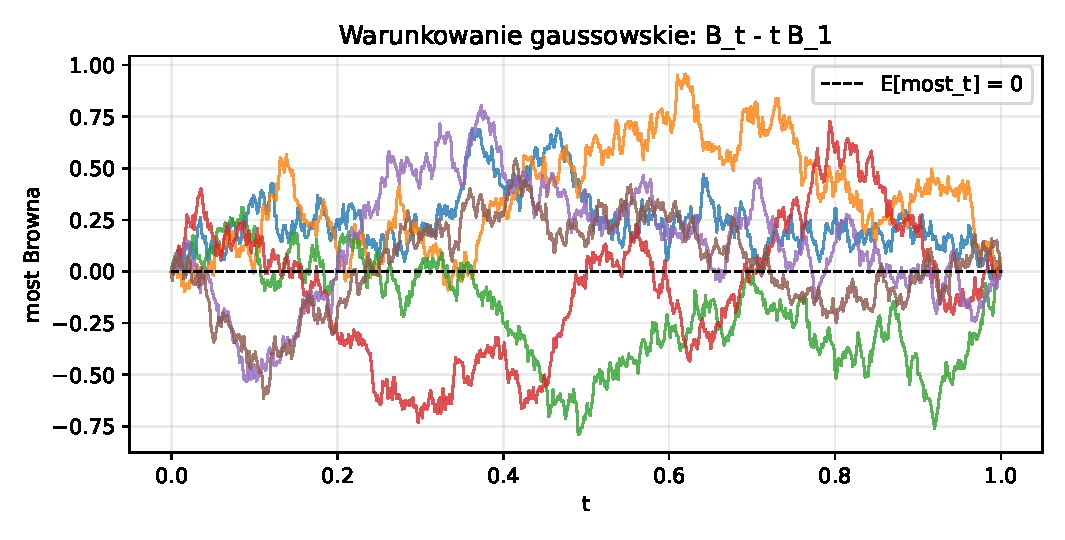
\includegraphics[width=0.88\textwidth]{figures/II_most_gaussowski.pdf}\par
\small\emph{Rysunek: Realizacje mostu gaussowskiego przywiązane do dwóch końców.}
\end{center}
\noindent\textbf{Kod w Pythonie (NumPy, Matplotlib).} Plik \texttt{code/II\_most\_gaussowski.py} można uruchomić niezależnie; zapisuje pokazany wykres.
\lstinputlisting[language=Python]{code/II_most_gaussowski.py}
% --- KONIEC ROZSZERZENIA ILUSTRACYJNEGO ---

\section{Podsumowanie: dlaczego procesy gaussowskie przygotowują ruch Browna?}\label{sec:volII:06:06}
Mamy już komplet narzędzi: jądro kowariancji pozwala skonstruować
prawo procesu, formuły warunkowe opisują predykcję, a
oszacowania momentów dają regularność trajektorii.
Następny rozdział pokaże, że prosty wzór $K(s,t)=\min(s,t)$
prowadzi do procesu o bardzo bogatych, a nawet zaskakujących
własnościach geometrycznych.

% ==============================================================
% TOM II — ROZDZIAŁ 7: PROCES WIENERA
% ==============================================================
\chapter{Proces Wienera: własności probabilistyczne i geometria trajektorii}
\label{chap:volII:07}
\par\smallskip\noindent{\small\textit{Powiązania:} sekcja~\ref{sec:volII:02:04} (konstrukcja Wienera); sekcja~\ref{sec:volII:13:01} (wariacja kwadratowa); \textup{tom~III}, sekcja~\ref{III-sec:volIII:01:01} (konstrukcja całki Wienera); twierdzenie~\ref{thm:volII:02:03} (istnienie procesu Wienera).}\par\smallskip

\label{ch:wiener}

\section{Od sum niezależnych przyrostów do ruchu Browna}\label{sec:volII:07:01}
Rozważmy błąd pomiaru, który narasta jako suma bardzo wielu drobnych,
w przybliżeniu niezależnych zakłóceń. W granicy czasowej spodziewamy
się procesu o przyrostach gaussowskich, którego wariancja rośnie
proporcjonalnie do długości przedziału. Tak powstaje matematyczna
motywacja standardowego procesu Wienera, czyli ruchu Browna.
Dla każdego $t$ mamy rozkład normalny, ale znacznie silniejszy
jest warunek \emph{niezależności przyrostów na rozłącznych
przedziałach}. To właśnie on odróżnia Wienera od dowolnego
procesu gaussowskiego.

\begin{definicja}[Standardowy proces Wienera]\label{def:volII:07:01}
Niech $(\Omega,\calF,\Prob)$ będzie przestrzenią probabilistyczną.
Proces rzeczywisty $W=(W_t)_{t\ge0}$ nazywamy
\emph{standardowym procesem Wienera} (\emph{standardowym ruchem Browna}),
jeżeli:
\begin{enumerate}
\item $W_0=0$ prawie na pewno;
\item jego trajektorie $t\mapsto W_t(\omega)$ są ciągłe dla prawie
wszystkich $\omega$;
\item dla dowolnych $0\le t_0<t_1<\cdots<t_n$ przyrosty
$W_{t_1}-W_{t_0},\ldots,W_{t_n}-W_{t_{n-1}}$
są wzajemnie niezależne;
\item $W_t-W_s\sim\Normal(0,t-s)$ dla wszystkich $0\le s<t$.
\end{enumerate}
Jeżeli ponadto zadano filtrację $(\calF_t)_{t\ge0}$, to $W$
nazywamy procesem Wienera \emph{względem tej filtracji},
gdy jest do niej adaptowany oraz $W_t-W_s$ jest niezależny
od $\calF_s$ dla wszystkich $s<t$.
\end{definicja}

Rozdział~\ref{ch:konstrukcja} dowiódł już istnienia takiego
procesu na pewnej przestrzeni probabilistycznej.
W dalszym ciągu możemy bez straty ogólności przyjąć,
że wszystkie jego trajektorie są ciągłe: modyfikujemy proces
na jednym zbiorze zerowym, przypisując na nim trajektorię zerową.
Takie ustalenie nie zmienia rozkładów skończeniewymiarowych.

\begin{twierdzenie}[Równoważna charakteryzacja gaussowska]\label{thm:volII:07:01}
Niech $X=(X_t)_{t\ge0}$ będzie rzeczywistym procesem
o prawie na pewno ciągłych trajektoriach. Wówczas $X$
jest standardowym procesem Wienera wtedy i tylko wtedy,
gdy jest procesem gaussowskim i dla wszystkich $s,t\ge0$
zachodzi
\[
\E X_t=0,\qquad \Cov(X_s,X_t)=\min(s,t).
\]
\end{twierdzenie}
\begin{proof}
Jeżeli $X=W$ jest procesem Wienera, to dla
$0=t_0<t_1<\cdots<t_n$ wektor $(W_{t_1},\ldots,W_{t_n})$
jest liniowym obrazem wektora niezależnych przyrostów normalnych,
więc jest gaussowski. Przy $s\le t$ korzystamy z rozkładu
$W_t=W_s+(W_t-W_s)$ oraz niezależności przyrostu od $W_s$:
$\Cov(W_s,W_t)=\Var(W_s)=s$. Średnie wynoszą zero.

Odwrotnie, $\Var(X_0)=K(0,0)=0$ i $\E X_0=0$,
a więc $X_0=0$ p.n. Dla $s<t$
$\Var(X_t-X_s)=t+s-2s=t-s$ i średnia przyrostu
jest zero. Jeżeli $[a,b]$ i $[c,d]$ są rozłączne oraz $b\le c$,
to $\Cov(X_b-X_a,X_d-X_c)=0$, co wynika z podstawienia
czterech wartości funkcji $\min(\cdot,\cdot)$.
Dowolne skończone rodziny takich przyrostów są wspólnie
gaussowskie, zatem ich zerowe kowariancje oznaczają niezależność.
Dostajemy wszystkie punkty definicji.
\end{proof}

\begin{przyklad}[Rozkład kilku obserwacji]
Dla $0<s<t$ wektor $(W_s,W_t)$ jest normalny dwuwymiarowo
ze średnią zero i macierzą kowariancji
$\left(\begin{smallmatrix}s&s\\s&t\end{smallmatrix}\right)$.
Jego współrzędne są zależne: $\Cov(W_s,W_t)=s$.
Jednak $W_s$ i $W_t-W_s$ są niezależne.
Dla $0<t_1<t_2<t_3$ mamy na przykład
\[
\Prob(W_{t_3}-W_{t_2}>a\mid W_{t_1}=x)
=1-\Phi\left(\frac{a}{\sqrt{t_3-t_2}}\right),
\]
gdzie równość rozumiana jest jako odpowiednia wersja
regularnego prawdopodobieństwa warunkowego.
Warunek na $W_{t_1}$ nie wpływa na późniejszy rozłączny przyrost.
Nie należy tego mylić z pytaniem o rozkład $W_{t_3}$,
który oczywiście zależy od stanu w chwili $t_1$.
\end{przyklad}

\section{Skalowanie, symetria i niezależność przyszłości}\label{sec:volII:07:02}
\begin{twierdzenie}[Symetrie i samopodobieństwo]\label{thm:volII:07:02}
Niech $W$ będzie procesem Wienera, a $c>0$.
Procesy $(c^{-1/2}W_{ct})_{t\ge0}$ i
$(-W_t)_{t\ge0}$ mają to samo prawo na przestrzeni
ciągłych trajektorii co $W$. Dla każdego $T>0$ proces
$(W_T-W_{T-t})_{0\le t\le T}$ ma prawo procesu Wienera
ograniczonego do $[0,T]$.
\end{twierdzenie}
\begin{proof}
Każdy z wymienionych procesów ma ciągłe trajektorie,
wartość początkową zero i jest gaussowski.
Dla pierwszego procesu kowariancja wynosi
$c^{-1}\min(cs,ct)=\min(s,t)$; dla drugiego
jest taka sama. Dla trzeciego, gdy $0\le s\le t\le T$,
przyrosty $W_T-W_{T-s}$ oraz $W_T-W_{T-t}$ mają
kowariancję $s$: wspólnym składnikiem są przyrosty
na przedziale $[T-s,T]$. Z poprzedniego twierdzenia
i jednoznaczności prawa procesu otrzymujemy tezy.
\end{proof}

\begin{uwaga}[Jak rozumieć skalowanie?]
Jeśli skala czasu rośnie $c$ razy, typowe wychylenie
rośnie $\sqrt c$ razy, a nie $c$ razy.
To odpowiada zależności $\Var(W_t)=t$.
Samopodobieństwo stanowi podstawę późniejszej zasady
niezmienniczości Donskera, wiążącej spacery losowe z
ruchem Browna.
\end{uwaga}

\begin{twierdzenie}[Własność Markowa i półgrupa przejścia]\label{thm:volII:07:03}
Niech $W$ będzie procesem Wienera względem filtracji
$(\calF_t)_{t\ge0}$. Dla dowolnych $s,t\ge0$
i ograniczonej mierzalnej funkcji $f:\R\to\R$ zachodzi
\[
\E[f(W_{s+t})\mid\calF_s]
=(P_tf)(W_s),\qquad
(P_tf)(x):=\int_\R f(x+y)p_t(y)\,\dd\lambda_1(y),
\]
gdzie $p_t(y)=(2\pi t)^{-1/2}\exp(-y^2/(2t))$ dla $t>0$,
a $P_0f=f$. Ponadto $P_{s+t}=P_sP_t$.
\end{twierdzenie}
\begin{proof}
Zapiszmy $W_{s+t}=W_s+Z$, gdzie $Z=W_{s+t}-W_s$
jest niezależna od $\calF_s$ i ma rozkład $\Normal(0,t)$.
Dla funkcji $f(x)=\ind{\{x\in A\}}$ własność
warunkowania niezależnej zmiennej daje żądany wzór.
Przez liniowość uzyskujemy go dla funkcji prostych, a
następnie przez zbieżność monotoniczną i rozkład na
części dodatnią i ujemną dla wszystkich ograniczonych
funkcji mierzalnych.
Aby udowodnić własność półgrupy, bierzemy niezależne
$Z_s\sim\Normal(0,s)$ i $Z_t\sim\Normal(0,t)$.
Ich suma ma rozkład $\Normal(0,s+t)$. Stąd
$P_s(P_tf)(x)=\E f(x+Z_s+Z_t)=P_{s+t}f(x)$;
przejścia $s=0$ lub $t=0$ są oczywiste.
\end{proof}

\section{Mocna własność Markowa: można zacząć od losowej chwili}\label{sec:volII:07:03}
Dla deterministycznej chwili $s$ przyszły przyrost
$W_{s+t}-W_s$ jest niezależny od $\calF_s$.
Prawdziwie nowa treść pojawia się przy \emph{losowej}
chwili $\tau$, np. pierwszym trafieniu w poziom $a$.
Nie można po prostu podstawić $s=\tau(\omega)$ w definicji
niezależności: musimy najpierw przybliżyć czas losowy
czasami przyjmującymi przeliczalnie wiele wartości.

\begin{twierdzenie}[Mocna własność Markowa procesu Wienera]\label{thm:volII:07:04}
Niech $W$ będzie procesem Wienera względem filtracji
$(\calF_t)_{t\ge0}$, a $\tau$ niech będzie względem niej
czasem zatrzymania takim, że $\Prob(\tau<\infty)=1$.
Wtedy proces $(W_{\tau+t}-W_\tau)_{t\ge0}$ jest
standardowym procesem Wienera i jest niezależny od
sigma-ciała $\calF_\tau$.
\end{twierdzenie}
\begin{proof}
Dla $n\ge1$ niech $h_n=2^{-n}$ i
$\tau_n=h_n\lceil\tau/h_n\rceil$.
Ponieważ $\{\tau_n\le t\}$ jest zdarzeniem określonym
przez warunek $\{\tau\le h_n\lfloor t/h_n\rfloor\}$,
czas $\tau_n$ jest czasem zatrzymania, przyjmuje wartości
w siatce $h_n\N_0$, spełnia $\tau\le\tau_n<\tau+h_n$
i zbiega do $\tau$ prawie na pewno.

Niech $A\in\calF_\tau$. Z nierówności $\tau\le\tau_n$
wynika $A\in\calF_{\tau_n}$. Ustalmy
$0\le t_1<\cdots<t_m$ i $u=(u_1,\ldots,u_m)\in\R^m$.
Dla zdarzenia $A\cap\{\tau_n=kh_n\}\in\calF_{kh_n}$
niezależność przyrostów po chwili $kh_n$ od tej
sigma-algebry daje
\begin{align*}
&\E\left[\ind{A\cap\{\tau_n=kh_n\}}
\exp\left(i\sum_{j=1}^m u_j(W_{\tau_n+t_j}-W_{\tau_n})\right)\right]\\
&\qquad=\Prob(A\cap\{\tau_n=kh_n\})
\exp\left(-\frac12\sum_{j,l=1}^m u_ju_l\min(t_j,t_l)\right).
\end{align*}
Sumujemy po $k\ge0$; jest to dozwolone przez
zbieżność zdominowaną, gdyż moduł każdego czynnika
wykładniczego nie przekracza $1$. Otrzymujemy
\[
\E\left[\ind A\exp\left(i\sum_j u_j
(W_{\tau_n+t_j}-W_{\tau_n})\right)\right]
=\Prob(A)\exp\left(-\frac12\sum_{j,l}
 u_ju_l\min(t_j,t_l)\right).
\]
Ciągłość trajektorii i $\tau_n\to\tau$ zapewniają
$W_{\tau_n+t_j}-W_{\tau_n}\to W_{\tau+t_j}-W_\tau$
prawie na pewno. Ponownie stosujemy zbieżność zdominowaną.
Otrzymana równość dla wszystkich $u$ oznacza, z jednoznaczności
funkcji charakterystycznych, że wektor przyszłych przyrostów
ma standardowy rozkład gaussowski i jest niezależny
od każdego $A\in\calF_\tau$. Niezależność
całej ciągłej trajektorii od $\calF_\tau$ wynika z faktu,
że borelowskie sigma-ciało przestrzeni ciągłych trajektorii
jest generowane przez odczyty w chwilach wymiernych.
Ciągłość przyszłych trajektorii wynika z ciągłości $W$.
\end{proof}

\begin{przyklad}[Co znaczy ``zapominanie'' w losowej chwili?]
Niech $a>0$ i $\tau_a=\inf\{t\ge0:W_t=a\}$.
Na zdarzeniu $\{\tau_a<\infty\}$ obserwator zna
całą przeszłą drogę oraz fakt, że cząstka właśnie dotarła
do $a$. Mocna własność Markowa mówi, że przyszły \emph{przyrost}
$W_{\tau_a+t}-a$ jest niezależnym, nowym ruchem Browna.
Nie oznacza to niezależności samego położenia $W_{\tau_a+t}$
od $W_{\tau_a}$, bo położenie zawiera znany punkt startowy.
\end{przyklad}

\section{Regularność trajektorii: ciągłość bez gładkości}\label{sec:volII:07:04}
Dla ustalonych $s<t$ przyrost ma skalę $\sqrt{t-s}$,
a nie $t-s$. Ta pozornie drobna różnica ma zasadniczy
skutek: trajektorie są ciągłe, ale prawie na pewno nie
mają pochodnej w żadnym punkcie.

\begin{twierdzenie}[Regularność H\"oldera poniżej $1/2$]\label{thm:volII:07:05}
Dla każdego $T>0$ i standardowego procesu Wienera $W$
zachodzi z prawdopodobieństwem $1$: dla każdego
$\gamma\in(0,1/2)$ istnieje losowa stała
$C_{\gamma,T}(\omega)<\infty$ taka, że
\[
|W_t(\omega)-W_s(\omega)|
\le C_{\gamma,T}(\omega)|t-s|^\gamma,
\qquad s,t\in[0,T].
\]
\end{twierdzenie}
\begin{proof}
Dla każdego $p>2$ i $s,t\in[0,T]$ mamy
$\E|W_t-W_s|^p=c_p|t-s|^{p/2}$.
Kryterium ciągłości Kołmogorowa daje modyfikację
o trajektoriach H\"oldera każdego rzędu
$\gamma<1/2-1/p$. Ponieważ zarówno $W$, jak i ta
modyfikacja mają ciągłe trajektorie, są nierozróżnialne;
możemy więc przypisać tę własność $W$.
Wybierając przeliczalny ciąg $p_k\to\infty$,
przecinamy zbiory o prawdopodobieństwie $1$ i
otrzymujemy jednocześnie wszystkie $\gamma<1/2$.
\end{proof}

\section{Wariacja kwadratowa: niezwykła wielkość trajektorii}\label{sec:volII:07:05}
Dla gładkiej funkcji $f$ i podziałów o coraz mniejszej
średnicy suma kwadratów przyrostów $\sum(\Delta f)^2$
dąży do zera. Dla Wienera dzieje się coś innego:
suma ta dąży do długości przedziału. To najważniejszy
mechanizm odróżniający rachunek Itô od klasycznego.

\begin{twierdzenie}[Wariacja kwadratowa procesu Wienera]\label{thm:volII:07:06}
Niech $W$ będzie standardowym procesem Wienera, $T>0$, zaś
$\pi_n=\{0=t_{0,n}<\cdots<t_{m_n,n}=T\}$
ciągiem deterministycznych podziałów $[0,T]$ o średnicy
$|\pi_n|:=\max_k(t_{k+1,n}-t_{k,n})\to0$.
Wówczas
\[
Q(\pi_n):=\sum_{k=0}^{m_n-1}
(W_{t_{k+1,n}}-W_{t_{k,n}})^2
\longrightarrow T\quad\text{w }L^2.
\]
Jeżeli $\pi_n$ jest podziałem dyadycznym, to zbieżność
zachodzi również prawie na pewno.
\end{twierdzenie}
\begin{proof}
Oznaczmy $\Delta_{k,n}=W_{t_{k+1,n}}-W_{t_{k,n}}$
oraz $h_{k,n}=t_{k+1,n}-t_{k,n}$.
Przyrosty są niezależne, $\Delta_{k,n}\sim\Normal(0,h_{k,n})$,
a $\E\Delta_{k,n}^2=h_{k,n}$ i
$\E\Delta_{k,n}^4=3h_{k,n}^2$. Zatem
$\Var(\Delta_{k,n}^2)=2h_{k,n}^2$.
Dzięki niezależności
\[
\E Q(\pi_n)=\sum_k h_{k,n}=T,
\qquad
\E\bigl|Q(\pi_n)-T\bigr|^2
=2\sum_k h_{k,n}^2\le 2T|\pi_n|\to0.
\]
Dla siatek dyadycznych $|\pi_n|=T2^{-n}$.
Nierówność Czebyszewa daje, dla każdego $\varepsilon>0$,
$\Prob(|Q(\pi_n)-T|>\varepsilon)
\le 2T^2 2^{-n}/\varepsilon^2$.
Suma po $n$ jest skończona, więc z pierwszego lematu
Borela--Cantellego odchylenie większe niż $\varepsilon$
występuje tylko skończenie wiele razy prawie na pewno.
Stosując to do $\varepsilon=1,1/2,1/3,\ldots$
i przecinając przeliczalnie wiele zdarzeń pełnej miary,
uzyskujemy $Q(\pi_n)\to T$ p.n.
\end{proof}

\begin{wniosek}[Jednostajna zbieżność wariacji kwadratowej]\label{cor:volII:07:01}
Dla podziałów dyadycznych $t_{k,n}=kT2^{-n}$
zdefiniujmy dla $t\in[0,T]$
\[
Q_n(t)=\sum_{k=0}^{2^n-1}
\bigl(W_{t\wedge t_{k+1,n}}-W_{t\wedge t_{k,n}}\bigr)^2.
\]
Wówczas $\sup_{0\le t\le T}|Q_n(t)-t|\to0$
prawie na pewno.
\end{wniosek}
\begin{proof}
Niech $h=T2^{-n}$ i
$Y_{k,n}=(W_{(k+1)h}-W_{kh})^2-h$.
Zmienne $Y_{k,n}$ są niezależne, wycentrowane i
$\sum_k\Var Y_{k,n}=2Th$.
Nierówność maksymalna Kołmogorowa daje
\[
\Prob\left(\max_{0\le j\le 2^n}
\left|\sum_{k<j}Y_{k,n}\right|>\varepsilon\right)
\le \frac{2Th}{\varepsilon^2}.
\]
Prawa strona jest sumowalna po $n$, więc maksimum
sum cząstkowych dąży do zera p.n. Gdy
$t\in[jh,(j+1)h]$, różnica między $Q_n(t)-t$
a sumą $\sum_{k<j}Y_{k,n}$ jest równa
$(W_t-W_{jh})^2-(t-jh)$. Jej moduł nie przekracza
$\max_j\sup_{u\in[jh,(j+1)h]}|W_u-W_{jh}|^2+h$.
Ta wielkość dąży do zera p.n. z jednostajnej
ciągłości trajektorii $W$ na $[0,T]$.
Połączenie obu oszacowań dowodzi tezy.
\end{proof}

\begin{wniosek}[Trajektorie nie mają skończonej wariacji całkowitej]\label{cor:volII:07:02}
Dla każdego $T>0$ trajektorie $t\mapsto W_t(\omega)$
mają z prawdopodobieństwem $1$ nieskończoną wariację
całkowitą na $[0,T]$. Prawie na pewno jest tak nawet
na każdym przedziale o dodatniej długości.
\end{wniosek}
\begin{proof}
Gdyby pewna ciągła trajektoria $w$ miała skończoną
wariację całkowitą $V$, to dla dowolnego podziału
$\sum_k(w(t_{k+1})-w(t_k))^2
\le\max_k|w(t_{k+1})-w(t_k)|\,V$.
Jednostajna ciągłość $w$ zapewnia zbieżność maksimum
przyrostów do zera wraz ze średnicą podziału.
Stąd suma kwadratów dążyłaby do zera, co przeczy
poprzedniemu twierdzeniu, dającemu granicę $T>0$.
Aby uzyskać twierdzenie dla wszystkich nietrywialnych
przedziałów jednocześnie, stosujemy ten sam dowód do
przedziałów o wymiernych końcach i przecinamy
przeliczalnie wiele zbiorów pełnej miary.
Każdy przedział o dodatniej długości zawiera taki
wymierny podprzedział; wariacja na większym przedziale
nie może być mniejsza od wariacji na mniejszym.
\end{proof}

\begin{przyklad}[Dlaczego lewy i środkowy punkt przedziału dają inne całki?]
Niech $t_k=kT/n$. Tożsamość algebraiczna
$W_{t_{k+1}}^2-W_{t_k}^2
=2W_{t_k}\Delta_kW+(\Delta_kW)^2$
daje
\[
\sum_{k=0}^{n-1}W_{t_k}(W_{t_{k+1}}-W_{t_k})
=\frac12W_T^2-\frac12\sum_{k=0}^{n-1}(\Delta_kW)^2
\longrightarrow \frac12(W_T^2-T)
\quad\text{w }L^2.
\]
Z kolei suma z uśrednieniem wartości na końcach
$\frac12(W_{t_k}+W_{t_{k+1}})$ spełnia
\[
\sum_{k=0}^{n-1}\frac{W_{t_k}+W_{t_{k+1}}}{2}
 (W_{t_{k+1}}-W_{t_k})=\frac12W_T^2
\]
\emph{dokładnie} dla każdego $n$.
To algebraiczny początek rozróżnienia całki Itô i
Stratonovicha. Pełna konstrukcja obu całek pojawi
się w części o rachunku stochastycznym.
\end{przyklad}


% --- ROZSZERZENIE ILUSTRACYJNE: II_wariacja ---
\subsection*{Eksperyment: kwadraty przyrostów kontra moduły}
Dla jednej trajektorii ruchu Browna na $[0,1]$ bierzemy zagnieżdżone
podziały dyadyczne $\pi_n=\{k/n:k=0,\ldots,n\}$, gdzie $n=2^m$.
Porównujemy sumy $Q_n=\sum_{k=0}^{n-1}(B_{(k+1)/n}-B_{k/n})^2$
oraz $V_n=\sum_{k=0}^{n-1}|B_{(k+1)/n}-B_{k/n}|$.
Pierwsze dążą do $1$ (przy rozważanych regularnych podziałach),
podczas gdy drugie nie są ograniczone dla typowej trajektorii.
Obie wielkości pokazujemy na różnych skalach pionowych.
\begin{center}
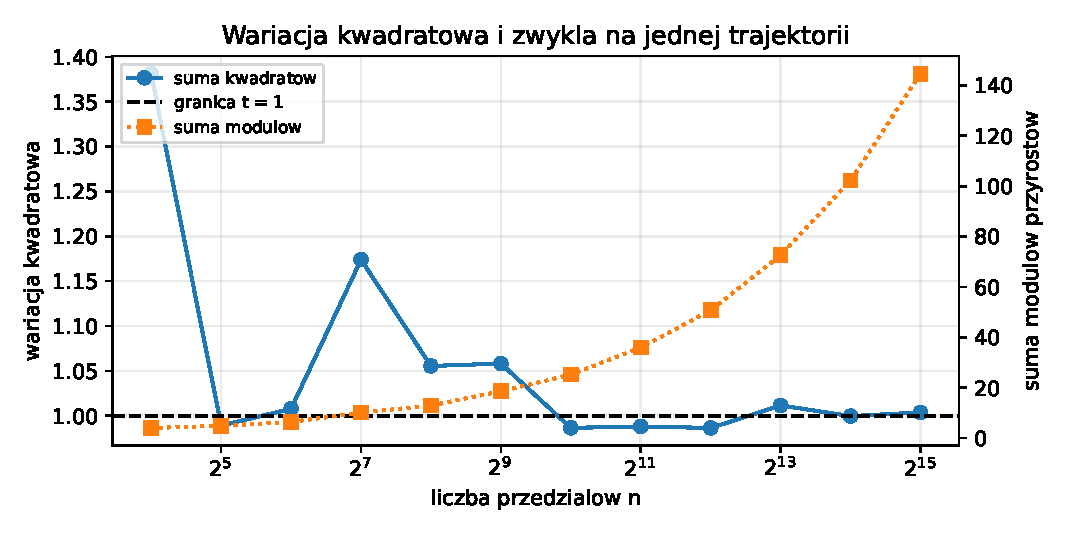
\includegraphics[width=0.88\textwidth]{figures/II_wariacja.pdf}\par
\small\emph{Rysunek: Różnica między wariacją kwadratową i sumą modułów przyrostów.}
\end{center}
\noindent\textbf{Kod w Pythonie (NumPy, Matplotlib).} Plik \texttt{code/II\_wariacja.py} można uruchomić niezależnie; zapisuje pokazany wykres.
\lstinputlisting[language=Python]{code/II_wariacja.py}
% --- KONIEC ROZSZERZENIA ILUSTRACYJNEGO ---

\section{Dlaczego ruch Browna nie ma pochodnej?}\label{sec:volII:07:06}
Brak skończonej wariacji całkowitej na każdym przedziale nie
wyklucza jeszcze pochodnej w pojedynczym punkcie. Potrzebny
jest silniejszy argument. Pokażemy, że na drobnej siatce
prawdopodobieństwo wystąpienia choćby trzech \emph{jednocześnie
bardzo małych} kolejnych przyrostów maleje wystarczająco szybko.
Gdyby trajektoria miała pochodną, takie trzy małe przyrosty
musiałyby się regularnie pojawiać blisko punktu różniczkowalności.

\begin{twierdzenie}[Nieróżniczkowalność trajektorii Wienera]\label{thm:volII:07:07}
Niech $W$ będzie standardowym procesem Wienera i $T>0$.
Wówczas z prawdopodobieństwem $1$ trajektoria
$t\mapsto W_t(\omega)$ nie jest różniczkowalna
w żadnym punkcie $t\in(0,T)$ i nie ma skończonej
pochodnej jednostronnej w punktach $0,T$.
\end{twierdzenie}
\begin{proof}
Ustalmy liczbę całkowitą $M\ge1$ i siatkę dyadyczną
o kroku $h_n=T2^{-n}$. Niech $A_n(M)$ oznacza zdarzenie,
że istnieje $k\in\{0,\ldots,2^n-3\}$, dla którego
trzy kolejne przyrosty
$\Delta_{k,n}W,\Delta_{k+1,n}W,\Delta_{k+2,n}W$
mają moduł nie większy niż $8Mh_n$.
Każdy z tych przyrostów ma rozkład $\Normal(0,h_n)$,
a są one niezależne. Z oszacowania gęstości standardowej
normalnej przez $1/\sqrt{2\pi}$ dostajemy
\[
\Prob(|\Delta_{k,n}W|\le8Mh_n)
=\Prob(|G|\le8M\sqrt{h_n})
\le \frac{16M}{\sqrt{2\pi}}\sqrt{h_n}.
\]
Stąd, z niezależności trzech przyrostów i sumowania
prawdopodobieństw po najwyżej $T/h_n$ pozycjach,
\[
\Prob(A_n(M))\le C\,M^3T\sqrt{h_n},
\]
gdzie $C$ jest stałą liczbową. Szereg po $n$ jest zbieżny,
więc lemat Borela--Cantellego daje
$\Prob(A_n(M)\text{ nieskończenie często})=0$.

Przypuśćmy teraz, że ciągła trajektoria $w$ ma skończoną
pochodną w pewnym $t\in(0,T)$. Z definicji pochodnej
istnieją $M\in\N$ i $\delta>0$ takie, że
$|w(s)-w(t)|\le M|s-t|$ dla $|s-t|<\delta$.
Dla dostatecznie dużego $n$ istnieje $k$ z
$kh_n\le t<(k+1)h_n$, a punkty
$kh_n,(k+1)h_n,(k+2)h_n,(k+3)h_n$
leżą w $(t-\delta,t+\delta)\cap[0,T]$.
Dla $j=0,1,2$ nierówność trójkąta daje
\[
|w((k+j+1)h_n)-w((k+j)h_n)|
\le M(|(k+j+1)h_n-t|+|(k+j)h_n-t|)
\le 8Mh_n.
\]
Zatem $A_n(M)$ zachodzi dla wszystkich dostatecznie
dużych $n$, w sprzeczności z poprzednim wnioskiem.
Przecinając zbiory pełnej miary po $M\in\N$,
wykluczamy wszystkie punkty różniczkowalności wewnątrz
$[0,T]$ naraz.

Dla końca $t=0$, istnienie skończonej pochodnej
prawostronnej oznaczałoby $|W_{h_n}|\le Mh_n$
dla pewnego całkowitego $M$ i wszystkich dużych $n$.
Jednak $\Prob(|W_{h_n}|\le Mh_n)\le C M\sqrt{h_n}$,
co jest sumowalne. Borel--Cantelli wyklucza taką
sytuację. W punkcie $T$ stosujemy analogiczny argument
do $W_T-W_{T-h_n}$. To kończy dowód.
\end{proof}

\begin{wniosek}[Próg wykładnika H\"oldera]\label{cor:volII:07:03}
Z prawdopodobieństwem $1$ na żadnym przedziale
$[a,b]\subset[0,\infty)$ o $a<b$ trajektoria Wienera
nie spełnia oszacowania
$|W_t-W_s|\le C|t-s|^\gamma$ dla wszystkich $s,t\in[a,b]$
z jakimkolwiek $C<\infty$ i $\gamma>1/2$.
\end{wniosek}
\begin{proof}
Gdyby takie oszacowanie zachodziło, to dla równomiernego
podziału na $n$ przedziałów suma kwadratów przyrostów
nie przekraczałaby $C^2(b-a)^{2\gamma}n^{1-2\gamma}$,
a więc dążyłaby do zera. To sprzeczne z dodatnią
wariacją kwadratową na każdym przedziale o wymiernych
końcach (przy niemal pewnym wspólnym zdarzeniu).
Każdy przedział $[a,b]$ z $a<b$ zawiera przedział
$[r,s]$ o wymiernych końcach i dodatniej długości;
oszacowanie H\"oldera na $[a,b]$ przeniosłoby się na
$[r,s]$. To daje sprzeczność.
\end{proof}

\begin{center}
\begin{tikzpicture}[x=0.9cm,y=0.8cm,>=Latex]
\draw[->] (-0.2,0)--(10.5,0) node[right] {$t$};
\draw[->] (0,-1.3)--(0,2.6) node[above] {$W_t$};
\draw[blue!75!black,thick] (0,0)--(0.45,0.55)--(0.8,0.18)--(1.18,1.05)--(1.55,0.82)--(1.83,1.5)--(2.14,0.9)--(2.5,1.1)--(2.86,0.22)--(3.2,0.67)--(3.45,0.08)--(3.75,-0.45)--(4.1,0.36)--(4.4,-0.05)--(4.7,0.78)--(5.04,0.42)--(5.37,1.2)--(5.65,0.66)--(5.95,1.3)--(6.25,0.55)--(6.56,0.1)--(6.86,0.88)--(7.21,0.47)--(7.5,1.22)--(7.83,1.0)--(8.15,1.72)--(8.53,1.03)--(8.85,1.4)--(9.2,0.82)--(9.6,1.65)--(10,1.15);
\draw[dashed,red!70!black] (0,1.42)--(10,1.42);
\node[red!70!black,above left] at (10,1.42) {$a$};
\draw[densely dotted,red!70!black] (1.80,0)--(1.80,1.42);
\node[below] at (1.80,0) {$\tau_a$};
\end{tikzpicture}
\par\smallskip\small Schemat trajektorii i pierwszego trafienia w poziom $a$.
Rysunek ma charakter poglądowy: prawdziwa trajektoria Wienera
jest ciągła, ale nie jest łamaną o skończonej liczbie odcinków.
\end{center}

\section{Pierwsze trafienie i zasada odbicia}\label{sec:volII:07:07}
\begin{definicja}[Czas pierwszego trafienia]\label{def:volII:07:02}
Niech $W$ będzie ciągłym procesem Wienera i $a>0$.
Definiujemy $\tau_a:=\inf\{t\ge0:W_t=a\}$,
przyjmując $\inf\varnothing=\infty$.
Dla naturalnej filtracji (lub dowolnej filtracji, do której
$W$ jest adaptowany) jest to czas zatrzymania, gdyż
$\{\tau_a\le t\}=\{\sup_{0\le s\le t}W_s\ge a\}$,
a supremum ciągłej trajektorii można obliczać po
chwilach wymiernych z $[0,t]$ wraz z końcem przedziału.
\end{definicja}

\begin{twierdzenie}[Zasada odbicia]\label{thm:volII:07:08}
Dla standardowego procesu Wienera $W$, $t>0$ i $a>0$
zachodzi
\[
\Prob\left(\sup_{0\le s\le t}W_s\ge a\right)
=2\Prob(W_t\ge a)
=2\left(1-\Phi\left(\frac{a}{\sqrt t}\right)\right),
\]
gdzie $\Phi$ jest dystrybuantą standardowego rozkładu normalnego.
\end{twierdzenie}
\begin{proof}
Niech $\tau=\tau_a$. Z ciągłości trajektorii
$\{\sup_{s\le t}W_s\ge a\}=\{\tau\le t\}$.
Jeśli $W_t>a$, to z ciągłości i $W_0=0<a$ musieliśmy
wcześniej osiągnąć $a$, zatem $\{W_t>a\}\subset\{\tau\le t\}$.

Na zdarzeniu $\{\tau\le t\}$ mamy $W_\tau=a$.
Z mocnej własności Markowa przyszły przyrost
$W_t-W_\tau$, przy zadanym $\calF_\tau$ i czasie
pozostałym $t-\tau$, ma symetryczny rozkład
$\Normal(0,t-\tau)$. Możemy to sformalizować,
warunkując najpierw względem $\calF_\tau$ i stosując
mocną własność Markowa do przyszłego procesu
$B_u=W_{\tau+u}-W_\tau$ oraz mierzalnej funkcji
$u=t-\tau$; fakt dla prostych $u$ przenosimy do
ogólnego $u$ przez aproksymację i ciągłość trajektorii.
Stąd
\[
\Prob(\tau\le t,\ W_t<a)
=\Prob(\tau\le t,\ W_t>a).
\]
Równość jest prawdziwa także na granicy $\tau=t$,
gdyż oba zdarzenia tam nie zachodzą.
Ponieważ $W_t$ ma rozkład ciągły,
$\Prob(W_t=a)=0$ i
$\Prob(\tau\le t,\ W_t>a)=\Prob(W_t>a)$.
Dzieląc $\{\tau\le t\}$ według zdarzeń
$\{W_t<a\},\{W_t=a\},\{W_t>a\}$,
dostajemy żądany wzór.
\end{proof}

\begin{wniosek}[Rozkład czasu trafienia]\label{cor:volII:07:04}
Dla $a>0$ czas $\tau_a$ jest skończony prawie na pewno,
a jego dystrybuanta i gęstość na $(0,\infty)$ mają postać
\[
\Prob(\tau_a\le t)=2\left(1-\Phi(a/\sqrt t)\right),
\qquad
f_{\tau_a}(t)=\frac{a}{\sqrt{2\pi}\,t^{3/2}}
\exp\left(-\frac{a^2}{2t}\right).
\]
Jednak $\E\tau_a=\infty$.
\end{wniosek}
\begin{proof}
Pierwszy wzór jest zasadą odbicia. Gdy $t\to\infty$,
argument $a/\sqrt t$ dąży do zera, więc dystrybuanta
dąży do $2(1-\Phi(0))=1$: czas jest skończony p.n.
Różniczkując dystrybuantę po $t>0$, dostajemy gęstość.
Ponadto, z twierdzenia o wartości średniej dla $\Phi$,
\[
\Prob(\tau_a>t)=2(\Phi(a/\sqrt t)-1/2)
\sim \sqrt{\frac2\pi}\frac{a}{\sqrt t}
\quad\text{gdy }t\to\infty.
\]
Dla nieujemnej zmiennej losowej zachodzi
$\E\tau_a=\int_0^\infty\Prob(\tau_a>t)\,\dd t$
(z twierdzenia Tonellego). Całka jest rozbieżna,
gdyż $\int_1^\infty t^{-1/2}\,\dd t=\infty$.
\end{proof}

\begin{uwaga}[Prawie pewne zakończenie nie daje skończonego średniego czasu]
Ruch Browna dociera do ustalonego dodatniego poziomu
z prawdopodobieństwem $1$, lecz wartość oczekiwana
czasu oczekiwania jest nieskończona.
To ważny kontrprzykład: nie wolno bez dodatkowych
warunków stosować próbkowania opcjonalnego bezpośrednio
w chwili $\tau_a$. Istnienie granicy $W_{\tau_a}=a$
prawie na pewno nie oznacza, że
$\E W_{\tau_a}=\E W_0$.
\end{uwaga}

\begin{zadanie}[Transformata Laplace'a czasu pierwszego trafienia]
Niech $W$ będzie procesem Wienera, $a>0$,
$\tau_a=\inf\{t\ge0:W_t=a\}$.
Obliczyć $\E e^{-\lambda\tau_a}$ dla $\lambda>0$.

\emph{Rozwiązanie.} Dla $\theta=\sqrt{2\lambda}>0$
proces $M_t=\exp(\theta W_t-\theta^2t/2)$
jest martyngałem: wynika to z niezależności przyrostów i
$\E e^{\theta(W_t-W_s)}=e^{\theta^2(t-s)/2}$.
Dla ograniczonego czasu $\tau_a\wedge n$ twierdzenie o
próbkowaniu opcjonalnym daje
$1=\E M_{\tau_a\wedge n}$.
Przed trafieniem w $a$ mamy $W_t<a$, a w chwili
trafienia $W_{\tau_a}=a$, więc
$0\le M_{\tau_a\wedge n}\le e^{\theta a}$.
Wiemy już, że $\tau_a<\infty$ p.n.; zatem
$M_{\tau_a\wedge n}\to\exp(\theta a-\lambda\tau_a)$
p.n. Zbieżność zdominowana pozwala przejść do granicy:
$1=e^{\theta a}\E e^{-\lambda\tau_a}$, skąd
\[
\E e^{-\lambda\tau_a}=e^{-a\sqrt{2\lambda}}.
\]
Ta transformata będzie w przyszłości użyteczna przy
porównywaniu ruchu Browna z procesami Lévy'ego.
\end{zadanie}

\section{Wyjście z przedziału: prawdopodobieństwa i średni czas}\label{sec:volII:07:08}
\begin{twierdzenie}[Wyjście procesu Wienera z $(-a,b)$]\label{thm:volII:07:09}
Niech $a,b>0$ oraz
$\tau:=\inf\{t\ge0:W_t\notin(-a,b)\}$.
Wtedy $\tau<\infty$ prawie na pewno,
$\E\tau=ab$ oraz
\[
\Prob(W_\tau=b)=\frac{a}{a+b},\qquad
\Prob(W_\tau=-a)=\frac{b}{a+b}.
\]
\end{twierdzenie}
\begin{proof}
Z ciągłości $W_{t\wedge\tau}\in[-a,b]$ i
$W_\tau\in\{-a,b\}$ na zdarzeniu $\{\tau<\infty\}$.
Z przyrostów gaussowskich wynika, że zarówno $W_t$,
jak i $W_t^2-t$ są martyngałami. Dla drugiego procesu
sprawdzamy bowiem, że przy $s<t$:
\[
\E[W_t^2-t\mid\calF_s]
=W_s^2+\E[(W_t-W_s)^2]-t=W_s^2-s,
\]
gdyż mieszany wyraz ma zerową warunkową wartość oczekiwaną.
Z próbkowania opcjonalnego w ograniczonej chwili
$t\wedge\tau$ dostajemy
$\E W_{t\wedge\tau}=0$ oraz
$\E W_{t\wedge\tau}^2=\E(t\wedge\tau)$.
Wprowadzając $M=\max(a,b)$, otrzymujemy
$\E(t\wedge\tau)\le M^2$. Zbieżność monotoniczna
przy $t\to\infty$ daje $\E\tau\le M^2<\infty$,
a więc $\tau<\infty$ p.n.

Ze zbieżności zdominowanej,
$W_{t\wedge\tau}\to W_\tau$ zarówno w $L^1$,
jak i w $L^2$; zatem
$\E W_\tau=0$ i
$\E W_\tau^2=\E\tau$.
Niech $p=\Prob(W_\tau=b)$. Ponieważ
$W_\tau$ przyjmuje tylko dwie wartości,
$0=\E W_\tau=bp-a(1-p)$, skąd $p=a/(a+b)$.
Następnie
\[
\E\tau=\E W_\tau^2
=b^2\frac{a}{a+b}+a^2\frac{b}{a+b}=ab.
\]
Wszystkie przejścia do granicy zostały więc uzasadnione
odpowiednio zbieżnością monotoniczną i zdominowaną.
\end{proof}

\begin{zadanie}[Start z dowolnego punktu przedziału]
Niech $x\in(-a,b)$, $a,b>0$, a proces
$X_t=x+W_t$. Obliczyć prawdopodobieństwo wyjścia
przez prawą krawędź i oczekiwany czas wyjścia.

\emph{Rozwiązanie.} Wyjście $X$ z $(-a,b)$ jest
równoważne wyjściu $W$ z przedziału
$(-a-x,b-x)$. W poprzednim twierdzeniu podstawiamy
$a'=a+x$, $b'=b-x$, obie liczby są dodatnie. Dostajemy
\[
\Prob(X_\tau=b)=\frac{a+x}{a+b},\qquad
\E\tau=(a+x)(b-x).
\]
Zwróćmy uwagę, że funkcja $u(x)=(a+x)(b-x)$
spełnia równanie $\frac12u''(x)=-1$ na $(-a,b)$
i warunki brzegowe $u(-a)=u(b)=0$.
Jest to pierwsza zapowiedź ścisłego związku procesów
Markowa z równaniami różniczkowymi.
\end{zadanie}

\section{Miara Wienera: całkowanie po wszystkich trajektoriach}\label{sec:volII:07:09}
Proces $W$ można opisywać dwojako. Dla ustalonej chwili $t$
zmienna $W_t$ jest normalna. Ale pojedynczy wynik
$\omega\in\Omega$ wyznacza także całą ciągłą funkcję
$t\mapsto W_t(\omega)$. Możemy zatem zapytać nie tylko
o prawdopodobieństwo $\{W_t\in A\}$, lecz także o
prawdopodobieństwo zdarzenia zależącego od całej drogi,
na przykład: ``trajektoria przez cały czas pozostaje
poniżej bariery'' lub ``pole pod trajektorią jest dodatnie''.

\begin{definicja}[Przestrzeń trajektorii i miara Wienera]\label{def:volII:07:03}
Dla $T>0$ definiujemy
\[
\calC_0([0,T]):=\{w\in C([0,T];\R):w(0)=0\},
\qquad \norm{w}_\infty=\sup_{0\le t\le T}|w(t)|.
\]
Niech $W$ będzie standardowym procesem Wienera o ciągłych
trajektoriach, traktowanym jako odwzorowanie
$W:\Omega\to\calC_0([0,T])$,
$W(\omega)(t)=W_t(\omega)$.
Jego \emph{prawem na przestrzeni trajektorii}, nazywanym
\emph{miarą Wienera}, jest miara probabilistyczna
$\mu_T:=\Prob\circ W^{-1}$ na
$(\calC_0([0,T]),\calB(\calC_0([0,T])))$.
\end{definicja}

\begin{stwierdzenie}[Mierzalność odwzorowania trajektorii]\label{prop:volII:07:01}
Jeżeli $W$ ma ciągłe trajektorie i każda zmienna $W_t$
jest mierzalna, to odwzorowanie
$\omega\mapsto W(\omega)\in\calC_0([0,T])$ jest mierzalne.
\end{stwierdzenie}
\begin{proof}
Dla każdej wymiernej chwili $r\in[0,T]$ odwzorowanie
ewaluacji $e_r(w)=w(r)$ jest ciągłe w normie supremum,
a $e_r\circ W=W_r$ jest mierzalne.
Przestrzeń $\calC_0([0,T])$ jest ośrodkową przestrzenią
metryczną (można przybliżać funkcje ciągłe łamanymi
o wymiernych węzłach i wymiernych wartościach).
Borelowskie sigma-ciało tej przestrzeni jest generowane
przez ewaluacje w przeliczalnym gęstym zbiorze chwil:
rzeczywiście $\norm{w-v}_\infty=\sup_{r\in D}|w(r)-v(r)|$
dla gęstego przeliczalnego $D$ zawierającego końce,
więc każda kula otwarta jest mierzalna względem
$\sigma(e_r:r\in D)$; dzięki ośrodkowości każdy zbiór
otwarty jest przeliczalną sumą takich kul.
Zatem przeciwobrazy zbiorów borelowskich przez $W$
są mierzalne.
\end{proof}

\begin{twierdzenie}[Całki cylindryczne względem miary Wienera]\label{thm:volII:07:10}
Niech $T>0$, $0<t_1<\cdots<t_m\le T$ oraz
$F:\R^m\to\R$ będzie funkcją borelowską, nieujemną
lub całkowalną względem rozkładu wektora
$(W_{t_1},\ldots,W_{t_m})$. Wówczas
\begin{align*}
&\int_{\calC_0([0,T])}F(w(t_1),\ldots,w(t_m))\,\dd\mu_T(w)\\
&\quad=\int_{\R^m}F(x_1,\ldots,x_m)
\prod_{k=1}^m p_{t_k-t_{k-1}}(x_k-x_{k-1})
\,\dd\lambda_m(x_1,\ldots,x_m),
\end{align*}
gdzie $t_0=0$, $x_0=0$ i $p_h(z)$ jest gęstością
$\Normal(0,h)$.
\end{twierdzenie}
\begin{proof}
Z definicji miary obrazowej całka po lewej jest równa
$\E F(W_{t_1},\ldots,W_{t_m})$.
Przeprowadzamy liniowe przekształcenie od przyrostów
$Z_k=W_{t_k}-W_{t_{k-1}}$ do kolejnych położeń
$x_k=Z_1+\cdots+Z_k$.
Przyrosty są niezależne, $Z_k$ mają gęstości
$p_{t_k-t_{k-1}}$, więc wektor $Z$ ma gęstość
będącą ich iloczynem. Macierz przekształcenia z $Z$
do $x$ jest trójkątna z jedynkami na przekątnej,
a zatem jej wyznacznik ma moduł $1$.
Wzór na zmianę zmiennych w całce Lebesgue'a
daje tezę. Dla $F\ge0$ dopuszczalność całkowania
wynika z twierdzenia Tonellego; w przypadku funkcji
całkowalnej stosujemy rozkład na części dodatnią i ujemną.
\end{proof}

\begin{zadanie}[Całka z całej trajektorii jako zmienna gaussowska]
Niech $A_T:=\int_0^T W_s\,\dd s$, gdzie całka jest zwykłą
całką Riemanna (równoważnie Lebesgue'a) z ciągłej trajektorii.
Obliczyć rozkład $A_T$ i jego funkcję charakterystyczną.

\emph{Rozwiązanie.} Aproksymujmy całkę sumami Riemanna
$A_T^{(n)}=\sum_{k=0}^{n-1}W_{kT/n}\,(T/n)$.
Każda suma jest gaussowska, ponieważ jest liniową
kombinacją wspólnie gaussowskich zmiennych.
Z ciągłości trajektorii $A_T^{(n)}\to A_T$ p.n.
Co więcej, jeśli $\varphi_n(s)$ jest lewym końcem
przedziału siatki zawierającego $s$, to nierówność
Cauchy'ego--Schwarza i twierdzenie Fubiniego dają
\begin{align*}
\E|A_T^{(n)}-A_T|^2
&\le T\int_0^T\E|W_{\varphi_n(s)}-W_s|^2\,\dd s\\
&\le T^2\frac{T}{n}\longrightarrow0.
\end{align*}
Zatem $A_T^{(n)}$ zbiega w $L^2$ do $A_T$,
a jego średnie i wariancje zbiegają do odpowiednich
wielkości granicy. Granica rozkładów normalnych o
zbieżnych parametrach jest normalna (wynika to wprost
ze zbieżności funkcji charakterystycznych).
Ponieważ $\E A_T=0$ i
\[
\Var(A_T)=\int_0^T\!\int_0^T\Cov(W_s,W_t)
\,\dd s\,\dd t
=\int_0^T\!\int_0^T\min(s,t)\,\dd s\,\dd t
=\frac{T^3}{3},
\]
dostajemy $A_T\sim\Normal(0,T^3/3)$ oraz
\[
\E e^{iuA_T}=\exp\left(-\frac{u^2T^3}{6}\right).
\]
W języku miary Wienera jest to dokładnie obliczenie
całki po trajektoriach
\[
\int_{\calC_0([0,T])}
\exp\left(iu\int_0^T w(s)\,\dd s\right)\,\dd\mu_T(w).
\]
\end{zadanie}

\begin{uwaga}[Trzy całki, których nie wolno utożsamiać]
Wyrażenie $\int_0^T W_s\,\dd s$ jest zwykłą całką
po czasie z jednej losowej, ciągłej funkcji.
Wyrażenie $\int_0^T H_s\,\dd W_s$ będzie całką
stochastyczną Itô, skonstruowaną później z przyrostów
procesu Wienera. Wreszcie
$\int_{\calC_0([0,T])}F(w)\,\dd\mu_T(w)$
całkuje funkcjonał $F$ \emph{po wszystkich możliwych
trajektoriach}. Jest to ścisła matematyczna całka Wienera
po drogach, stanowiąca punkt wyjścia do wzoru
Feynmana--Kaca. Oscylacyjna całka Feynmana w czasie
rzeczywistym wymaga odrębnej analizy i nie jest
zwykłą całką względem miary probabilistycznej.
\end{uwaga}


\begin{stwierdzenie}[Most Browna i miara Wienera mają różne prawa]\label{prop:volII:07:02}
Dla $T>0$ niech $\mu_T$ będzie miarą Wienera na
$\calC_0([0,T])$, a $\nu_T$ prawem mostu Browna
$\beta_t=W_t-(t/T)W_T$. Wtedy $\mu_T$ i $\nu_T$
są wzajemnie singularne.
\end{stwierdzenie}
\begin{proof}
Zbiór $A=\{w\in\calC_0([0,T]):w(T)=0\}$ jest domknięty,
więc borelowski. Ponieważ $\beta_T=0$, mamy $\nu_T(A)=1$.
Natomiast $W_T\sim\Normal(0,T)$ ma rozkład bezatomowy,
więc $\mu_T(A)=\Prob(W_T=0)=0$. Jest to definicja
wzajemnej singularności miar.
\end{proof}

\begin{uwaga}[Jaki typ zbieżności wariacji kwadratowej udowodniono?]
Dla \emph{dowolnych deterministycznych} podziałów
$[0,T]$ o średnicy zmierzającej do zera wykazaliśmy
zbieżność sum kwadratów przyrostów w $L^2$, a zatem
według prawdopodobieństwa. Zbieżność prawie na pewno
uzyskaliśmy dla \emph{konkretnego ciągu siatek dyadycznych}.
Z tych dwóch zdań nie wolno wyciągać wniosku, że
zbieżność prawie na pewno zachodzi dla każdej dowolnie
wybranej sekwencji podziałów. Ważne jest również,
czy podziały wolno wybierać zależnie od trajektorii.
\end{uwaga}

\section{Równanie ciepła i generator ruchu Browna}\label{sec:volII:07:10}
\begin{twierdzenie}[Generator i równanie ciepła]\label{thm:volII:07:11}
Niech $(P_t)_{t\ge0}$ będzie półgrupą zdefiniowaną wzorem
$(P_tf)(x)=\E f(x+W_t)$ dla ograniczonych borelowskich
$f:\R\to\R$. Wówczas:
\begin{enumerate}
\item dla każdej $f\in C_b^3(\R)$, czyli funkcji o
ciągłych i ograniczonych pochodnych do rzędu trzeciego,
zachodzi dla każdego $x\in\R$
\[
\lim_{t\downarrow0}\frac{(P_tf)(x)-f(x)}{t}
=\frac12 f''(x);
\]
\item jeżeli $f\in C_b(\R)$, to funkcja
$u(t,x)=(P_tf)(x)$ jest klasy $C^{1,2}$ na
$(0,\infty)\times\R$, spełnia
$\partial_tu=\frac12\partial_{xx}u$
oraz $u(t,x)\to f(x)$ dla każdego $x$ przy $t\downarrow0$.
\end{enumerate}
\end{twierdzenie}
\begin{proof}
Dla $f\in C_b^3(\R)$ wzór Taylora z resztą daje
\[
f(x+h)=f(x)+hf'(x)+\frac12h^2f''(x)+R(x,h),\qquad
|R(x,h)|\le\frac{\norm{f'''}_\infty}{6}|h|^3.
\]
Podstawmy $h=W_t\sim\Normal(0,t)$ i uśrednijmy.
Mamy $\E W_t=0$, $\E W_t^2=t$ i
$\E|W_t|^3=c_3t^{3/2}$. Zatem
$|(P_tf)(x)-f(x)-tf''(x)/2|
\le \norm{f'''}_\infty c_3t^{3/2}/6$.
Po podzieleniu przez $t$ reszta dąży do zera,
co dowodzi pierwszej części.

Dla $t>0$ możemy zapisać
$u(t,x)=\int_\R f(y)p_t(y-x)\,\dd\lambda_1(y)$.
Na każdym przedziale czasowym $t\in[\delta,R]$
($0<\delta<R$) pochodne jądra gaussowskiego
$\partial_t p_t(z)$, $\partial_zp_t(z)$ i
$\partial_{zz}p_t(z)$ są ograniczone przez całkowalne
funkcje zmiennej $z$, niezależne od $t$ w tym przedziale.
Wynika to z jawnej postaci pochodnych, będących
wielomianami w $z$ pomnożonymi przez
$\exp(-z^2/(2R))$, z odpowiednimi stałymi.
Twierdzenie o różniczkowaniu pod znakiem całki daje
istnienie i ciągłość wskazanych pochodnych $u$.
Bezpośredni rachunek gęstości wykazuje
$\partial_t p_t(z)=\frac12\partial_{zz}p_t(z)$,
a więc po przeniesieniu pochodnych pod całkę
$\partial_tu=\frac12\partial_{xx}u$.

Na koniec $W_t\to0$ według prawdopodobieństwa,
bo $\E W_t^2=t\to0$. Dla ustalonego $x$ i
$\varepsilon>0$ ciągłość $f$ w $x$ daje $\delta>0$
takie, że $|f(x+z)-f(x)|<\varepsilon$ dla $|z|<\delta$.
Dzieląc wartość oczekiwaną według $|W_t|<\delta$
i jego dopełnienia, otrzymujemy
$|P_tf(x)-f(x)|\le\varepsilon
+2\norm f_\infty\Prob(|W_t|\ge\delta)\to\varepsilon$.
Dowolność $\varepsilon$ daje wymaganą zbieżność.
\end{proof}

\begin{przyklad}[Od losowej trajektorii do równania różniczkowego]
Dla $f(x)=\cos(kx)$, $k\in\R$, mamy
$P_tf(x)=\E\cos(kx+kW_t)
=e^{-k^2t/2}\cos(kx)$.
Rzeczywiście, część urojona funkcji charakterystycznej
rozkładu $\Normal(0,t)$ znika, a część rzeczywista
wynosi $e^{-k^2t/2}$. Jednocześnie
$\partial_tu=-(k^2/2)u$ i
$\frac12\partial_{xx}u=-(k^2/2)u$.
Jeden rachunek probabilistyczny dostarcza więc
jawnego rozwiązania równania ciepła.
\end{przyklad}

\section{Podsumowanie i kierunek dalszej teorii}\label{sec:volII:07:11}
Proces Wienera łączy zaskakujące fakty: ma ciągłe
trajektorie, ale żadna z nich nie jest różniczkowalna;
ma nieskończoną wariację całkowitą, lecz jego wariacja
kwadratowa jest dokładnie równa upływającemu czasowi.
Jednocześnie można go analizować za pomocą elementarnych
narzędzi gaussowskich, mocnej własności Markowa i
równania ciepła.

Przygotowaliśmy również przestrzeń trajektorii i miarę Wienera.
Dalsze rozdziały rozwiną całki po drogach, ruch Browna
w wielu wymiarach i ścisły rachunek stochastyczny.
W szczególności wzór Feynmana--Kaca połączy
ważone miary trajektorii z półgrupami operatorów
Schrödingera, a całka Itô zbuduje matematyczne
narzędzia do równań różniczkowych stochastycznych.


% ==============================================================
% ROZDZIAŁ 8. ROZSZERZENIE TEORII RUCHU BROWNA
% ==============================================================
\chapter{Ruch Browna w wielu wymiarach i dalsze własności trajektorii}
\label{chap:volII:08}
\par\smallskip\noindent{\small\textit{Powiązania:} sekcja~\ref{sec:volII:07:02} (skalowanie Wienera); \textup{tom~I}, sekcja~\ref{I-sec:volI:05:02} (nierówności momentowe); \textup{tom~III}, sekcja~\ref{III-sec:volIII:03:06} (wielowymiarowy wzór Itô); twierdzenie~\ref{thm:volII:07:02} (symetrie procesu Wienera).}\par\smallskip

\label{ch:brown-multi}

\section{Dlaczego potrzebujemy procesu wielowymiarowego?}\label{sec:volII:08:01}
W ruchu jednowymiarowym możemy badać przekroczenie bariery przez
cząstkę. Ruch w przestrzeni fizycznej wymaga jednak opisu wielu
współrzędnych naraz. Pytania zmieniają się wtedy jakościowo:
jak długo cząstka pozostaje w kuli? Czy dociera do wyróżnionego
punktu? Jak zmieniają się wyniki po obróceniu układu współrzędnych?
Zacznijmy od konstrukcji, w której odpowiedź na ostatnie pytanie
wynika ze szczególnej postaci macierzy kowariancji.

\begin{definicja}[Standardowy wielowymiarowy ruch Browna]\label{def:volII:08:01}
Niech $d\in\N$. Proces $B=(B_t)_{t\ge0}$ o wartościach
w $\R^d$, z prawie na pewno ciągłymi trajektoriami, nazywamy
\emph{standardowym $d$-wymiarowym ruchem Browna}, jeżeli
$B_0=0$ prawie na pewno, ma niezależne przyrosty oraz
$B_t-B_s\sim\Normal_d(0,(t-s)I_d)$ dla wszystkich $0\le s<t$.
Jeżeli $x\in\R^d$, proces $X_t=x+B_t$ nazywamy ruchem Browna
rozpoczynającym się w $x$; jego prawo i wartość oczekiwaną oznaczamy
odpowiednio przez $\Prob_x$ oraz $\E_x$.
\end{definicja}

\begin{twierdzenie}[Konstrukcja i izotropia]\label{thm:volII:08:01}
Dla każdego $d\ge1$ istnieje standardowy $d$-wymiarowy ruch
Browna $B$. Jego współrzędne są niezależnymi standardowymi
procesami Wienera, a dla $1\le i,j\le d$ i $s,t\ge0$
\[
\E B_t^{(i)}=0,\qquad
\Cov(B_s^{(i)},B_t^{(j)})=\delta_{ij}\min(s,t).
\]
Jeżeli $U\in\R^{d\times d}$ jest macierzą ortogonalną,
to proces $(UB_t)_{t\ge0}$ ma to samo prawo na
$C_0([0,T];\R^d)$ co $B$, dla każdego $T>0$.
\end{twierdzenie}
\begin{proof}
Na przestrzeni iloczynowej $d$ kopii przestrzeni probabilistycznej
z ruchem Browna weźmy niezależne procesy $W^{(1)},\ldots,W^{(d)}$
i połóżmy $B_t=(W_t^{(1)},\ldots,W_t^{(d)})$.
Wektor każdego przyrostu ma niezależne współrzędne o rozkładzie
$\Normal(0,t-s)$, czyli ma rozkład $\Normal_d(0,(t-s)I_d)$.
Współrzędne na różnych rozłącznych przedziałach także są niezależne;
można to zobaczyć, grupując skończone wektory przyrostów po
współrzędnych. Ciągłość wynika z przecięcia $d$ zdarzeń pełnej miary.
Ponieważ $U((t-s)I_d)U^\top=(t-s)I_d$, przyrosty procesu $UB$
mają te same rozkłady co przyrosty $B$ i pozostają niezależne.
Stąd równość rozkładów skończeniewymiarowych, a przez mierzalność
ewaluacji na przestrzeni trajektorii także równość praw na
$C_0([0,T];\R^d)$.
\end{proof}

\begin{uwaga}[Niezależność współrzędnych a niezależność położenia]
Współrzędne $B_t^{(1)},\ldots,B_t^{(d)}$ są niezależne w ustalonej
chwili $t$. Nie wynika stąd, że położenia $B_s$ i $B_t$ są niezależne
dla $s<t$: przeciwnie, mają wspólną przeszłość, a ich kowariancja
wynosi $sI_d$. Niezależne są \emph{przyrosty} na rozłącznych
przedziałach czasu.
\end{uwaga}

\begin{twierdzenie}[Generator i wielowymiarowe równanie ciepła]\label{thm:volII:08:02}
Niech $B$ będzie standardowym ruchem Browna w $\R^d$.
Dla $t\ge0$ oraz ograniczonej funkcji borelowskiej
$f:\R^d\to\R$ połóżmy $P_tf(x)=\E f(x+B_t)$.
Jeżeli $f\in C_b^3(\R^d)$ (wszystkie pochodne do rzędu trzeciego
są ciągłe i ograniczone), to dla każdego $x\in\R^d$
\[
\lim_{t\downarrow0}\frac{P_tf(x)-f(x)}{t}=\frac12\Delta f(x).
\]
Jeżeli $f\in C_b(\R^d)$, to $u(t,x)=P_tf(x)$ jest klasy
$C^{1,2}$ na $(0,\infty)\times\R^d$, spełnia
$\partial_tu=\frac12\Delta u$ oraz $u(t,x)\to f(x)$ dla $t\downarrow0$.
\end{twierdzenie}
\begin{proof}
Z wielowymiarowego wzoru Taylora z resztą, ograniczeniem
pochodnych trzeciego rzędu i normą euklidesową dostajemy
$f(x+h)=f(x)+\langle\nabla f(x),h\rangle+
\frac12 h^\top D^2f(x)h+R_x(h)$, gdzie
$|R_x(h)|\le C_d\max_{|\alpha|=3}\|\partial^\alpha f\|_\infty|h|^3$.
Ponieważ $\E B_t=0$,
$\E[B_t^{(i)}B_t^{(j)}]=t\delta_{ij}$ i
$\E|B_t|^3=t^{3/2}\E|B_1|^3$, otrzymujemy
$P_tf(x)-f(x)=\frac{t}{2}\sum_i\partial_{ii}f(x)+O(t^{3/2})$.
To dowodzi granicy po podzieleniu przez $t$.
Dla $t>0$ rozkład $B_t$ ma gęstość
$p_t^{(d)}(z)=(2\pi t)^{-d/2}\exp(-|z|^2/(2t))$.
Na każdym pasie czasowym $\delta\le t\le R$ pochodne
$\partial_t p_t^{(d)}$ oraz $\partial_i p_t^{(d)}$,
$\partial_{ij}p_t^{(d)}$ są zdominowane całkowalnymi
funkcjami zmiennej $z$ (wielomian razy gaussowski ogon).
Różniczkując splot $u(t,x)=\int_{\R^d} f(x+z)p_t^{(d)}(z)\,\dd\lambda_d(z)$
po jądrze, dostajemy $\partial_tu=\frac12\Delta u$.
Zbieżność do warunku początkowego wynika z ciągłości $f$ w $x$,
ograniczenia $f$ i faktu $\E|B_t|^2=dt\to0$, dokładnie jak
w dowodzie jednowymiarowym.
\end{proof}

\begin{przyklad}[Ruch Browna z anizotropową kowariancją]
Niech $A\in\R^{m\times d}$, $b\in\R^m$ i $X_t=b+AB_t$.
Wówczas $X_t-X_s\sim\Normal_m(0,(t-s)AA^\top)$ i
$\E X_t=b$. Jeżeli $AA^\top$ jest dodatnio określona, ale nie jest wielokrotnością
macierzy jednostkowej, kierunki nie są równoważne: powierzchnie
jednakowej gęstości są elipsoidami. Dla
$f\in C_b^3(\R^m)$ generator ma postać
$Lf=\frac12\sum_{i,j}(AA^\top)_{ij}\partial_{ij}f$.
Jeżeli $AA^\top$ jest osobliwa, proces porusza się w
odpowiedniej podprzestrzeni afinicznej; gęstość względem
$\lambda_m$ nie musi istnieć.
\end{przyklad}


\begin{zadanie}[Anizotropowa dyfuzja w płaszczyźnie]
Niech $B=(B^{(1)},B^{(2)})$ będzie standardowym ruchem Browna
w $\R^2$ i niech $X_t=(2B_t^{(1)},B_t^{(2)})$.
Wyznaczyć rozkład $X_t$, generator procesu i prawdopodobieństwo
$\Prob(|X_t^{(1)}|>2a)$ dla $a,t>0$.

\emph{Rozwiązanie.} Macierz $A=\operatorname{diag}(2,1)$ daje
$AA^\top=\operatorname{diag}(4,1)$. Zatem
$X_t\sim\Normal_2(0,t\operatorname{diag}(4,1))$,
a jego gęstość wynosi
$ (4\pi t)^{-1}\exp(-x_1^2/(8t)-x_2^2/(2t))$.
Generator ma postać $Lf=2\partial_{11}f+\tfrac12\partial_{22}f$.
Wreszcie
$\Prob(|X_t^{(1)}|>2a)=\Prob(|B_t^{(1)}|>a)
=2(1-\Phi(a/\sqrt t))$.
Współczynnik dyfuzji w pierwszym kierunku jest cztery razy
większy niż w drugim; nie można go odczytać z samej
wartości oczekiwanej $\E X_t=0$.
\end{zadanie}

\section{Czas wyjścia z kuli i martyngał kwadratu promienia}\label{sec:volII:08:02}
\begin{twierdzenie}[Średni czas wyjścia z kuli]\label{thm:volII:08:03}
Niech $d\in\N$, $R>0$, $x\in\R^d$ i $|x|<R$.
Dla standardowego $d$-wymiarowego ruchu Browna $B$ połóżmy
$X_t=x+B_t$ oraz $\tau=\inf\{t\ge0:|X_t|\ge R\}$.
Wtedy $\tau<\infty$ prawie na pewno i
\[
\E\tau=\frac{R^2-|x|^2}{d}.
\]
\end{twierdzenie}
\begin{proof}
Dla $s<t$ i $Z=B_t-B_s$, niezależnego od przeszłości,
$\E Z=0$ i $\E|Z|^2=d(t-s)$. Rozwinięcie kwadratu daje
$\E[|X_t|^2\mid\calF_s]=|X_s|^2+d(t-s)$.
Zatem $M_t=|X_t|^2-dt$ jest martyngałem.
Dla każdego deterministycznego $n\in\N$ zatrzymujemy go
w ograniczonej chwili $\tau\wedge n$ (twierdzenie o
próbkowaniu opcjonalnym daje)
\[
\E|X_{\tau\wedge n}|^2-|x|^2=d\E(\tau\wedge n).
\]
Z ciągłości trajektorii zawsze $|X_{\tau\wedge n}|\le R$:
przed $\tau$ proces jest w kuli, a w chwili $\tau<\infty$
osiąga jej sferę. Stąd $d\E(\tau\wedge n)\le R^2$.
Zbieżność monotoniczna daje $\E\tau\le R^2/d<\infty$,
co wymusza $\tau<\infty$ p.n. Wtedy
$|X_{\tau\wedge n}|^2\to|X_\tau|^2=R^2$ p.n., a
zmienne są ograniczone przez $R^2$. Zbieżność zdominowana
i monotoniczna po obu stronach poprzedniej tożsamości dają
$R^2-|x|^2=d\E\tau$.
\end{proof}

\begin{zadanie}[Wyjście z dysku]
Rozważmy standardowy dwuwymiarowy ruch Browna, którego
położenie początkowe ma odległość $r<R$ od środka dysku
promienia $R$. Ile średnio trzeba czekać na pierwsze osiągnięcie
okręgu?

\emph{Rozwiązanie.} Z twierdzenia dla $d=2$ dostajemy
$\E\tau=(R^2-r^2)/2$. Gdy $r=0$, średni czas to $R^2/2$.
Zależność od $r$ jest kwadratowa, mimo że typowe wychylenie
po czasie $t$ ma rząd $\sqrt t$.
\end{zadanie}

\section{Maksimum, zasada odbicia i rozkład końcowego położenia}\label{sec:volII:08:03}
W rozdziale poprzednim wyprowadziliśmy prawdopodobieństwo
przekroczenia poziomu $a$ do chwili $T$. Często potrzebujemy
więcej: co wiemy o położeniu końcowym, jeśli poziom został
po drodze osiągnięty?

\begin{twierdzenie}[Rozkład łączny maksimum i położenia]\label{thm:volII:08:04}
Niech $W$ będzie standardowym procesem Wienera,
$T>0$, $a>0$ i $M_T:=\sup_{0\le s\le T}W_s$.
Wówczas dla dowolnego borelowskiego $A\subset(-\infty,a)$
\[
\Prob(M_T<a,\ W_T\in A)
=\int_A\bigl(p_T(y)-p_T(2a-y)\bigr)\,\dd\lambda_1(y),
\]
gdzie $p_T(y)=(2\pi T)^{-1/2}\exp(-y^2/(2T))$.
Ponadto $M_T$ ma ten sam rozkład co $|W_T|$ oraz
$\E M_T=\sqrt{2T/\pi}$.
\end{twierdzenie}
\begin{proof}
Niech $\tau_a$ będzie chwilą pierwszego trafienia w $a$.
Dla trajektorii z $\tau_a\le T$ odbijamy część drogi
po chwili $\tau_a$ według wzoru
$\widetilde W_t=W_t$ dla $t\le\tau_a$ oraz
$\widetilde W_t=2a-W_t$ dla $t>\tau_a$.
Mocna własność Markowa oraz symetria przyrostów po
$\tau_a$ pokazują, że to przekształcenie zachowuje prawo
procesu na zdarzeniu $\{\tau_a\le T\}$. Dokładniej,
dla dowolnego ograniczonego funkcjonału borelowskiego
$H$ ciągłej trajektorii warunkujemy względem $\calF_{\tau_a}$:
po odbiciu niezależny przyszły proces Wienera ma nadal to samo prawo.
W szczególności
$\Prob(M_T\ge a,W_T\in A)=\Prob(W_T\in 2a-A)$,
bo $A\subset(-\infty,a)$, a trajektorie kończące się
w $2a-A\subset(a,\infty)$ muszą wcześniej trafić w $a$.
Gęstość końcowego położenia wynosi $p_T$, zaś gęstość
drugiego zdarzenia po zmianie zmiennej to $p_T(2a-y)$.
Odejmując od $\Prob(W_T\in A)$, otrzymujemy wzór.
Ponieważ $\Prob(M_T\ge a)=2\Prob(W_T\ge a)$,
dystrybuanta $M_T$ na $[0,\infty)$ jest dystrybuantą
$|W_T|$. Stąd
$\E M_T=\E|W_T|=\sqrt{2T/\pi}$.
\end{proof}

\begin{wniosek}[Maksimum mostu Browna]\label{cor:volII:08:01}
Niech $\beta_t=W_t-(t/T)W_T$ dla $0\le t\le T$.
Dla każdego $a>0$ zachodzi
\[
\Prob\left(\sup_{0\le t\le T}\beta_t\le a\right)
=1-\exp\left(-\frac{2a^2}{T}\right).
\]
\end{wniosek}
\begin{proof}
Z rozdziału o procesach gaussowskich wiemy, że $\beta$ jest
niezależny od $W_T$. Dla każdego $y\in\R$ proces
$\beta_t+(t/T)y$ ma rozkład warunkowy całej trajektorii
Wienera przy $W_T=y$; jest to \emph{regularna wersja}
rozkładu warunkowego, a nie warunkowanie na zdarzeniu o
prawdopodobieństwie dodatnim.

Niech $V=\sup_{0\le t\le T}\beta_t$ i dla $y<b$ połóżmy
$H(y,b)=\Prob(\sup_{0\le t\le T}(\beta_t+ty/T)<b)$.
Z poprzedniego twierdzenia, przez podzielenie gęstości
wspólnej zdarzenia braku przekroczenia i położenia końcowego
przez $p_T(y)>0$, otrzymujemy dla prawie każdego $y<b$
\[
H(y,b)=1-\frac{p_T(2b-y)}{p_T(y)}.
\]
Wyrażenie po prawej stronie ma dla $y\to0$ granicę
$g(b):=1-\exp(-2b^2/T)$, o ile $b>0$.

Ustalmy $a>0$ i $0<\varepsilon<a$. Jeśli $|y|<\varepsilon$,
to dla każdej trajektorii $\sup_t|(t/T)y|\le\varepsilon$.
Dlatego mamy zawieranie zdarzeń prowadzące do nierówności
\[
H(y,a-\varepsilon)\le\Prob(V<a)
\le H(y,a+\varepsilon).
\]
Możemy wybrać ciąg $y_k\to0$ spoza sumy dwóch zbiorów
wyjątkowych miary Lebesgue'a zero, odpowiadających progom
$a-\varepsilon$ i $a+\varepsilon$. Podstawienie wzoru
na $H$ i przejście do granicy daje
$g(a-\varepsilon)\le\Prob(V<a)\le g(a+\varepsilon)$.
Ponieważ $g$ jest ciągła, po $\varepsilon\downarrow0$
otrzymujemy $\Prob(V<a)=g(a)$. Wreszcie
$\{V\le a\}=\bigcap_{n\ge1}\{V<a+1/n\}$;
ciągłość miary z góry i ciągłość $g$ dają
$\Prob(V\le a)=g(a)$. Dowód przy okazji wykazał,
że $\Prob(V=a)=0$ dla każdego $a>0$.
\end{proof}


\begin{uwaga}[Dlaczego przejście $y\to0$ nie jest tautologią?]
Dla ciągłej zmiennej $W_T$ zdarzenie $\{W_T=0\}$ ma
prawdopodobieństwo zero. Reguła Bayesa dla zdarzeń o dodatniej
mierze nie daje zatem rozkładu mostu przy zerowym punkcie
końcowym. Poprzedni dowód najpierw konstruuje \emph{konkretną}
wersję warunkowego prawa przy każdym $y$ przez rozkład
Gaussowski, a następnie wykorzystuje ciągłość przesunięcia
trajektorii o funkcję $ty/T$. Wartość w $y=0$ jest tym
samym uzasadniona przez tę wersję, nie przez arbitralne
podstawienie do tożsamości obowiązującej tylko prawie wszędzie.
\end{uwaga}

\begin{zadanie}[Maksimum ruchu Browna w jednostce czasu]
Niech $W$ będzie standardowym procesem Wienera.
Obliczyć $\Prob(\sup_{0\le s\le1}W_s\ge1)$ oraz
$\E\sup_{0\le s\le1}W_s$.

\emph{Rozwiązanie.} Z zasady odbicia pierwsze
prawdopodobieństwo wynosi $2(1-\Phi(1))\approx0{,}3173$.
Wartość oczekiwana maksimum to $\sqrt{2/\pi}$.
Obserwujemy, że $\Prob(W_1\ge1)=1-\Phi(1)$ jest dwa razy
mniejsze: część trajektorii zdążyła osiągnąć próg,
a później wróciła poniżej niego.
\end{zadanie}


\begin{zadanie}[Warunkowy rozkład położenia mostu w dwóch wymiarach]
Niech $B$ będzie standardowym ruchem Browna w $\R^2$.
Wyznaczyć regularny rozkład warunkowy $B_1$ przy $B_4=y$,
gdzie $y=(2,-2)$, a następnie obliczyć prawdopodobieństwo,
że pierwsza współrzędna $B_1$ jest dodatnia.

\emph{Rozwiązanie.} Nie wolno dzielić przez $\Prob(B_4=y)=0$.
Korzystamy z rozkładu warunkowego wektorów gaussowskich.
Mamy $\Cov(B_1,B_4)=I_2$ oraz $\Var(B_4)=4I_2$.
Średnia warunkowa jest więc równa $I_2(4I_2)^{-1}y=y/4$,
a kowariancja wynosi
$I_2-I_2(4I_2)^{-1}I_2=\tfrac34 I_2$.
Zatem
\[
\Law(B_1\mid B_4=y)=\Normal_2\!\left(\frac{y}{4},\frac34 I_2\right).
\]
Dla $y=(2,-2)$ pierwsza współrzędna ma rozkład
$\Normal(1/2,3/4)$, skąd
$\Prob(B_1^{(1)}>0\mid B_4=y)=\Phi(1/\sqrt3)$.
Wynik opisuje \emph{wersję} warunkowania określoną
przez ciągłą funkcję parametru $y$.
\end{zadanie}

\begin{zadanie}[Warunkowanie położenia procesu Wienera w środku przedziału]
Niech $W$ będzie standardowym procesem Wienera. Wyznaczyć
regularny rozkład warunkowy $W_1$ przy $W_2=y$ oraz
obliczyć $\Prob(W_1>0\mid W_2=2)$ w wybranej wersji
rozkładu warunkowego.

\emph{Rozwiązanie.} Wektor $(W_1,W_2)$ jest gaussowski,
$\Var(W_1)=1$, $\Var(W_2)=2$ i
$\Cov(W_1,W_2)=1$. Wzór na warunkowanie wektorów
gaussowskich daje
\[
\Law(W_1\mid W_2=y)=\Normal(y/2,1/2).
\]
Nie dzielimy przez $\Prob(W_2=y)$, bo jest ono zerowe:
wykorzystujemy regularną wersję warunkowego rozkładu.
Przy $y=2$ otrzymujemy
\[
\Prob(W_1>0\mid W_2=2)=\Phi(\sqrt 2).
\]
Średnia warunkowa $y/2$ jest liniową interpolacją
między punktem początkowym $0$ i zaobserwowanym punktem
$y$; nie znaczy to jednak, że cała trajektoria mostu
jest deterministyczną prostą. Warunkowa wariancja jest
dodatnia i wynosi $1/2$.
\end{zadanie}

\section{Oscylacje drogi na dowolnie małych przedziałach}\label{sec:volII:08:04}
\begin{twierdzenie}[Natychmiastowe oscylacje przy zadanej chwili]\label{thm:volII:08:05}
Niech $W$ będzie standardowym procesem Wienera i niech
$t_0\ge0$ będzie ustaloną deterministyczną chwilą.
Wtedy z prawdopodobieństwem $1$ dla każdego $\varepsilon>0$
istnieją $s_+,s_-\in(t_0,t_0+\varepsilon)$ takie, że
$W_{s_+}>W_{t_0}$ oraz $W_{s_-}<W_{t_0}$.
\end{twierdzenie}
\begin{proof}
Proces $B_s=W_{t_0+s}-W_{t_0}$ jest standardowym
ruchem Browna. Dla każdego $r>0$ i $a>0$ zasada odbicia
daje
$\Prob(\sup_{0\le s\le r}B_s\ge a)=2(1-\Phi(a/\sqrt r))$.
Gdy $a\downarrow0$, prawdopodobieństwo to dąży do $1$.
Z ciągłości miary dla rosnących zdarzeń dostajemy
$\Prob(\sup_{0\le s\le r}B_s>0)=1$.
Ta sama własność dla $-B$ daje
$\Prob(\inf_{0\le s\le r}B_s<0)=1$.
Przecinamy zdarzenia pełnej miary dla $r=1/n$,
$n\in\N$. Z tego wynika teza dla wszystkich
$\varepsilon>0$, przez wybór $1/n<\varepsilon$.
\end{proof}

\begin{uwaga}[Nie wolno zamienić ``każda ustalona chwila'' na ``wszystkie chwile'']
Udowodnione zdarzenie pełnej miary zależy od $t_0$.
Na ogół nie wolno przecinać nieprzeliczalnie wielu
zbiorów pełnej miary. Własność stwierdzona w twierdzeniu
nie zachodzi jednocześnie dla wszystkich chwil trajektorii:
na przykład w chwili ścisłego maksimum na przedziale
$[0,T]$ nie może wystąpić większa wartość przed końcem
tego przedziału. To ważna lekcja dotycząca kwantyfikatorów
w twierdzeniach o trajektoriach.
\end{uwaga}


\section{Rozkład promienia i oszacowania ryzyka wyjścia}\label{sec:volII:08:05}
\begin{twierdzenie}[Rozkład odległości od początku]\label{thm:volII:08:06}
Niech $B$ będzie standardowym ruchem Browna w $\R^d$
i $t>0$. Wtedy $|B_t|^2/t$ ma rozkład $\chi^2_d$,
a w szczególności
$\E|B_t|^2=dt$ i $\Var(|B_t|^2)=2dt^2$.
\end{twierdzenie}
\begin{proof}
Z definicji współrzędne $B_t^{(i)}/\sqrt t$ są niezależnymi
zmiennymi o rozkładzie $\Normal(0,1)$. Zatem
$|B_t|^2/t=\sum_{i=1}^d(B_t^{(i)}/\sqrt t)^2$,
co jest definicją rozkładu $\chi^2_d$.
Każdy składnik kwadratowy ma średnią $1$ i wariancję $2$,
a niezależność pozwala dodać momenty i wariancje.
\end{proof}

\begin{zadanie}[Oszacowanie prawdopodobieństwa wyjścia z sześcianu]
Niech $B$ będzie standardowym ruchem Browna w $\R^d$, $a,T>0$.
Oszacować $\Prob(\exists t\in[0,T]:\max_i|B_t^{(i)}|\ge a)$.

\emph{Rozwiązanie.} Jeśli proces opuszcza sześcian $(-a,a)^d$,
to dla pewnej współrzędnej $i$ zachodzi
$\sup_{t\le T} B_t^{(i)}\ge a$ lub
$\inf_{t\le T} B_t^{(i)}\le-a$.
Z nierówności sumy i zasady odbicia,
\[
\Prob\bigl(\sup_{t\le T}\|B_t\|_\infty\ge a\bigr)
\le4d\bigl(1-\Phi(a/\sqrt T)\bigr).
\]
Możemy zastąpić prawą stronę jej minimum z $1$.
Oszacowanie jest proste, choć nie musi być ostre,
ponieważ wielokrotnie zlicza trajektorie przekraczające
kilka ścian sześcianu.
\end{zadanie}

\section{Schematyczny rysunek procesu dwuwymiarowego}\label{sec:volII:08:06}
\begin{center}
\begin{tikzpicture}[x=0.85cm,y=0.85cm,>=Latex]
 \draw[->,gray] (-3.2,0)--(3.7,0) node[right] {$x_1$};
 \draw[->,gray] (0,-2.5)--(0,2.7) node[above] {$x_2$};
 \draw[blue!70!black,very thick,rounded corners=1pt]
 (0,0)--(.15,.3)--(.45,.1)--(.1,.6)--(.3,.9)--(-.1,1.15)--(-.7,.9)
 --(-.55,.4)--(-.9,.2)--(-.4,-.2)--(-.8,-.7)--(-1.2,-.5)
 --(-1.45,-.85)--(-1.1,-1.1)--(-1.7,-1.4)--(-1.3,-1.7)
 --(-2.1,-1.5)--(-1.85,-1.1)--(-2.25,-.65)--(-1.9,-.25)
 --(-2.6,.2)--(-2.15,.6)--(-2.55,1.05)--(-2.1,1.3);
 \fill[red!75!black] (0,0) circle (2pt) node[below right] {$B_0$};
 \fill[blue!70!black] (-2.1,1.3) circle (2pt) node[above] {$B_T$};
 \draw[->,blue!70!black,thick] (-2.55,1.05)--(-2.1,1.3);
\end{tikzpicture}
\par\smallskip\small Schemat dwóch współrzędnych ruchu Browna w płaszczyźnie.
Łamana jest jedynie ilustracją: niemal każda rzeczywista trajektoria
jest ciągła i nieróżniczkowalna.
\end{center}


% ==============================================================
% ROZDZIAŁ 9. PROCESY ODNOWY
% ==============================================================
\chapter{Procesy odnowy: zliczanie zdarzeń bez własności braku pamięci}
\label{chap:volII:09}
\par\smallskip\noindent{\small\textit{Powiązania:} sekcja~\ref{sec:volII:04:02} (proces Poissona); \textup{tom~I}, sekcja~\ref{I-sec:volI:08:01} (prawa wielkich liczb); sekcja~\ref{sec:volII:05:02} (czasy oczekiwania); twierdzenie~\ref{thm:volII:04:02} (charakterystyka procesu Poissona).}\par\smallskip

\label{ch:renewal}

\section{Dlaczego proces Poissona nie opisuje każdego strumienia zdarzeń?}\label{sec:volII:09:01}
W procesie Poissona po dowolnym czasie obserwacji oczekiwanie na
kolejne zdarzenie ma nadal rozkład wykładniczy. To wynika z własności
braku pamięci. Awaria mechanizmu, którego prawdopodobieństwo
uszkodzenia rośnie z wiekiem, nie ma jednak na ogół tej własności.
Potrzebujemy więc modelu z niezależnymi, ale niekoniecznie
wykładniczymi czasami między kolejnymi zdarzeniami.
\emph{Proces odnowy} opisuje liczbę ukończonych cykli, w których
po każdym odnowieniu system zaczyna działać jak nowy.

\begin{definicja}[Proces odnowy]\label{def:volII:09:01}
Niech $(T_n)_{n\ge1}$ będzie ciągiem niezależnych zmiennych
losowych o jednakowym rozkładzie $F$ na $(0,\infty)$, przy czym
$T_n>0$ prawie na pewno. Definiujemy $S_0=0$,
$S_n=\sum_{k=1}^nT_k$ oraz, dla $t\ge0$,
\[
N_t:=\sup\{n\ge0:S_n\le t\}\in\N_0\cup\{\infty\}.
\]
Proces $N=(N_t)_{t\ge0}$ nazywamy \emph{procesem odnowy}.
Liczby $S_n$ to chwile odnowień, a $T_n=S_n-S_{n-1}$
to czasy pomiędzy odnowieniami. Gdy $T_n\sim\mathrm{Exp}(\lambda)$,
odzyskujemy proces Poissona o intensywności $\lambda$.
\end{definicja}

\begin{twierdzenie}[Brak eksplozji i podstawowe prawdopodobieństwa]\label{thm:volII:09:01}
Dla procesu odnowy z poprzedniej definicji, dla każdego $t\ge0$,
$N_t<\infty$ prawie na pewno. W szczególności proces ma
niemalejące, prawostronnie ciągłe trajektorie, które w skończonym
czasie wykonują skończenie wiele skoków wielkości $1$.
Dla $n\in\N_0$ zachodzi
\[
\Prob(N_t\ge n)=\Prob(S_n\le t),\qquad
\Prob(N_t=n)=\Prob(S_n\le t)-\Prob(S_{n+1}\le t).
\]
Dla $n\ge1$ dystrybuantą $S_n$ jest $n$-krotny splot $F^{*n}$.
\end{twierdzenie}
\begin{proof}
Ponieważ $\Prob(T_1>0)=1$, istnieje $\varepsilon>0$
takie, że $p:=\Prob(T_1\ge\varepsilon)>0$.
Zmienne $I_k=\ind{\{T_k\ge\varepsilon\}}$ są niezależne
i mają wspólny rozkład Bernoulliego z parametrem $p$.
Z mocnego prawa wielkich liczb
$n^{-1}\sum_{k=1}^n I_k\to p>0$ prawie na pewno.
Ponieważ $S_n\ge\varepsilon\sum_{k=1}^nI_k$, wynika stąd
$S_n\to\infty$ prawie na pewno; dlatego $N_t$ jest skończone
prawie na pewno. Na każdym przedziale $[0,t]$ jest zatem
skończenie wiele punktów skoku $S_1,\dots,S_{N_t}$,
a definicja $N_t=\sum_{n\ge1}\ind{\{S_n\le t\}}$
daje prawostronną ciągłość.
Równość zdarzeń $\{N_t\ge n\}=\{S_n\le t\}$ jest bezpośrednia;
odejmując prawdopodobieństwa kolejnych zagnieżdżonych zdarzeń,
uzyskujemy drugi wzór. Rozkład sumy niezależnych zmiennych
ma dystrybuantę będącą splotem ich rozkładów.
\end{proof}

\begin{uwaga}[Warunek $T_n>0$ jest istotny]
Gdyby dopuszczano $\Prob(T_1=0)>0$, lecz nadal
$\Prob(T_1>0)>0$, nie doszłoby do eksplozji, ale mogłyby
wystąpić wielokrotne skoki w tej samej chwili.
Założenie dodatniości usuwa ten problem i upraszcza zapis.
Jeżeli zaś $T_1=0$ prawie na pewno, wszystkie odnowienia
nastąpiłyby w chwili zerowej, a $N_0=\infty$.
\end{uwaga}

\begin{stwierdzenie}[Skończona średnia liczby odnowień]\label{prop:volII:09:01}
Dla każdego procesu odnowy z $T_1>0$ prawie na pewno i każdego
$t<\infty$ zachodzi $\E N_t<\infty$, nawet gdy $\E T_1=\infty$.
\end{stwierdzenie}
\begin{proof}
Ustalmy $\theta>0$. Liczba
$r=\E e^{-\theta T_1}$ spełnia $0<r<1$.
Z nierówności Markowa i niezależności
\[
\Prob(S_n\le t)=\Prob(e^{-\theta S_n}\ge e^{-\theta t})
\le e^{\theta t}\E e^{-\theta S_n}=e^{\theta t}r^n.
\]
Z tożsamości $N_t=\sum_{n\ge1}\ind{\{S_n\le t\}}$
i twierdzenia Tonellego otrzymujemy
$\E N_t=\sum_{n\ge1}\Prob(S_n\le t)
\le e^{\theta t}r/(1-r)<\infty$.
\end{proof}

\begin{center}
\begin{tikzpicture}[x=1cm,y=0.55cm,>=Latex]
\draw[->] (0,0)--(11,0) node[right] {$t$};
\draw[->] (0,0)--(0,5.8) node[above] {$N_t$};
\draw[very thick,blue!70!black]
(0,0)--(1.6,0) (1.6,1)--(3.8,1) (3.8,2)--(4.8,2)
(4.8,3)--(8,3) (8,4)--(10.2,4);
\foreach \x/\y in {1.6/0,3.8/1,4.8/2,8/3}{
 \draw[blue!70!black,very thick] (\x,\y)--(\x,{\y+1});
 \fill[blue!70!black] (\x,{\y+1}) circle (2pt);
 \draw[dashed,gray] (\x,0)--(\x,\y);
}
\foreach \x/\t in {1.6/1,3.8/2,4.8/3,8/4}{
 \node[below] at (\x,0) {$S_{\t}$};
}
\foreach \y in {1,2,3,4}{\node[left] at (0,\y) {$\y$};}
\end{tikzpicture}
\par\smallskip\small Schemat procesu odnowy. Odstępy
$T_1=S_1$, $T_2=S_2-S_1$, $T_3=S_3-S_2$ nie muszą mieć rozkładu
wykładniczego; dlatego liczba odnowień na rozłącznych przedziałach
zwykle nie jest niezależna.
\end{center}

\begin{przyklad}[Deterministyczny cykl]
Jeżeli $T_n\equiv c>0$, to $S_n=nc$ i
$N_t=\lfloor t/c\rfloor$. W modelu Poissona
$\Var(N_t)=\E N_t$, tutaj zaś $\Var(N_t)=0$.
Proces odnowy obejmuje więc zarówno modele losowe, jak i
całkowicie regularne cykle. Przykład pokazuje, że sam parametr
$1/\E T_1$ nie opisuje charakteru fluktuacji.
Ten deterministyczny proces jest jednak procesem Markowa
(w sensie niejednorodnym w czasie): znając aktualną chwilę,
znamy bez losowości wszystkie jego przyszłe wartości.
Nie może więc służyć jako dowód, że ogólny proces odnowy
nie ma własności Markowa. Rzeczywisty kontrprzykład podajemy dalej.
\end{przyklad}


\begin{twierdzenie}[Proces odnowy nie musi być procesem Markowa]\label{thm:volII:09:02}
Niech $(T_n)_{n\ge1}$ będą niezależnymi zmiennymi, dla których
$\Prob(T_n=1)=\Prob(T_n=2)=1/2$, i niech
$N_t=\sup\{n\ge0:\sum_{k=1}^nT_k\le t\}$.
Wtedy proces $(N_t)_{t\ge0}$ \emph{nie jest} procesem Markowa
względem swojej filtracji naturalnej
$\mathcal F_t^N=\sigma(N_s:0\le s\le t)$.
\end{twierdzenie}
\begin{proof}
Spójrzmy na chwile $1$, $5/2$ i $13/4$.
Rozważmy dwa zdarzenia należące do $\mathcal F_{5/2}^N$:
\[
A=\{N_1=1,N_{5/2}=1\},\qquad
D=\{N_1=0,N_{5/2}=1\}.
\]
Oba mają dodatnie prawdopodobieństwo.
Na $A$ koniecznie $T_1=1$ i $T_2=2$: gdyby
$T_2=1$, druga odnowa nastąpiłaby już w chwili $2$.
Zatem $S_2=3<13/4$ i
$\Prob(N_{13/4}\ge2\mid A)=1$.
Na $D$ mamy $T_1=2$, a $T_2$ nadal przyjmuje wartości
$1$ i $2$ z jednakowymi prawdopodobieństwami,
niezależnie od $D$. Stąd
$\Prob(N_{13/4}\ge2\mid D)=1/2$.

Na obu zdarzeniach obecny stan $N_{5/2}$ jest taki sam,
mianowicie równy $1$. Gdyby $N$ miał własność Markowa,
warunkowe prawdopodobieństwo zdarzenia
$\{N_{13/4}\ge2\}$ przy całej informacji do chwili $5/2$
byłoby funkcją wyłącznie $N_{5/2}$. Jego średnie
warunkowe na $A$ i $D$ musiałyby więc być równe.
Obliczone wartości $1$ i $1/2$ przeczą temu warunkowi.
\end{proof}

\begin{uwaga}[Stan trzeba czasem poszerzyć]
Sama liczba odnowień $N_t$ nie mówi, ile czasu upłynęło
od ostatniej odnowy. To właśnie brakująca informacja w
powyższym dowodzie. Para $(N_t,A_t)$, gdzie
$A_t=t-S_{N_t}$, jest naturalnym kandydatem na stan
procesu Markowa: po znajomości wieku rozkład czasu
pozostałego do nowego cyklu można obliczyć z ogona
rozkładu odstępów. Własność Markowa takiej pary
wymaga osobnego sformułowania i dowodu; jej nie
utożsamiamy z własnością Markowa samego $N_t$.
\end{uwaga}


\begin{twierdzenie}[Wiek odnowy przywraca własność Markowa]\label{thm:volII:09:03}
\label{thm:wiek-markow}
Niech $T_1,T_2,\ldots$ będą niezależnymi, jednakowo rozłożonymi
zmiennymi o wartościach w $(0,\infty)$, o dystrybuancie $F$,
a $N_t$ i $A_t=t-S_{N_t}$ oznaczają liczbę odnowień i wiek
ostatniego cyklu. Wówczas $Y_t=(N_t,A_t)$ jest jednorodnym
w czasie procesem Markowa względem filtracji naturalnej
$\calF_t^N=\sigma(N_s:0\le s\le t)$.
Dokładniej, dla $u\ge0$, na zdarzeniu $\{N_t=n,A_t=a\}$
(rozumianym przez regularny rozkład warunkowy) resztkowy czas
$R_t$ ma ogon
$\overline F(a+u)/\overline F(a)$, gdy $\overline F(a)>0$,
a po następnym odnowieniu proces jest zbudowany z nowych,
niezależnych odstępów o prawie $F$. Opis ten nie zależy od $t$.
\end{twierdzenie}
\begin{proof}
Ustalmy deterministyczne $t$. Z trajektorii $(N_s)_{0\le s\le t}$
można odzyskać wszystkie chwile skoków $S_k\le t$, a więc
$N_t$ i $S_{N_t}$ są $\calF_t^N$-mierzalne. Na zdarzeniu
$\{N_t=n\}$ znamy $T_1,\ldots,T_n$, natomiast o $T_{n+1}$
wiemy tylko, że $T_{n+1}>t-S_n=A_t$. Istotnie,
$\{N_t=n\}=\{S_n\le t,\ T_{n+1}>t-S_n\}$.
Dla ustalonego $n$ i dowolnej ograniczonej funkcji borelowskiej
$\psi$ warunkowanie względem $T_1,\ldots,T_n$ oraz
niezależność $T_{n+1}$ dają
\[
\E[\psi(T_{n+1}-A_t)\mid\calF_t^N]
=\frac{\E[\psi(T_1-A_t)\ind{\{T_1>A_t\}}]}{\overline F(A_t)}
\quad\text{na }\{N_t=n,\ \overline F(A_t)>0\}.
\]
Równość można zweryfikować przez przemnożenie przez dowolną
ograniczoną funkcję dotychczasowych chwil skoków i całkowanie;
uzyskujemy w ten sposób wersję warunkową, bez dzielenia przez
prawdopodobieństwo zdarzenia $\{A_t=a\}$.
Przyszłe zmienne $T_{n+2},T_{n+3},\ldots$ są niezależne zarówno
od tej informacji, jak i od $T_{n+1}$. Po upływie resztkowego
czasu kolejna liczba odnowień oraz wiek procesu są zatem
jednoznacznymi funkcjami tych niezależnych odstępów i
aktualnej pary $(n,a)$. Dla dowolnej ograniczonej funkcji
borelowskiej $h$ na $\N_0\times[0,\infty)$ istnieje więc
funkcja $P_uh(n,a)$, która nie zależy od chwili $t$ i spełnia
$\E[h(Y_{t+u})\mid\calF_t^N]=P_uh(Y_t)$.
To jest żądana jednorodna własność Markowa.
Co istotne, nie wystarczy znać tylko rozkładu $R_t$:
po następnej odnowie całą przyszłość wyznaczają nowe,
niezależne odstępy. Właśnie ta niezależność pozwala
przejść od opisu pierwszego kolejnego skoku do dowolnej
liczby dalszych odnowień.
W szczególności, jeżeli do chwili $t+u$ nie ma nowej odnowy,
to $Y_{t+u}=(n,a+u)$; prawdopodobieństwo tego zdarzenia
jest równe $\overline F(a+u)/\overline F(a)$ przy
$\overline F(a)>0$. Zdarzenie $\{\overline F(A_t)=0\}$
ma jednak prawdopodobieństwo zero: dla każdego $n$ z niezależności
$T_{n+1}$ od $(T_1,\ldots,T_n)$ wynika
\[
\begin{aligned}
&\Prob\bigl(N_t=n,\,\overline F(A_t)=0\bigr)\\
&=\E\bigl[\ind{\{S_n\le t,\,\overline F(t-S_n)=0\}}
     \Prob(T_{n+1}>t-S_n\mid T_1,\ldots,T_n)\bigr]=0.
\end{aligned}
\]
Sumując po $n$, uzasadniamy, że iloraz wystarcza na całym
zdarzeniu pełnej miary. Dla wartości $(n,a)$ spoza nośnika
rozkładu pary $(N_t,A_t)$ jądro warunkowe można określić
dowolnie; nie zmienia to własności Markowa.
\end{proof}

\begin{zadanie}[Dlaczego sam licznik nie wystarcza?]
Niech odstępy między odnowieniami mają rozkład jednostajny
na $[1,2]$. Ustalmy $t=2$ i rozważmy dwa możliwe przebiegi
z $N_t=1$: w pierwszym ostatnia odnowa nastąpiła w chwili
$t-1/4$, w drugim w chwili $t-3/4$. Porównać prawdopodobieństwa
braku odnowy w następnych $1/2$ jednostki czasu.

\emph{Rozwiązanie.} Dla wieku $a$ ogon pozostałego czasu
wynosi $\overline F(a+1/2)/\overline F(a)$.
Przy $a=1/4$ mamy $\overline F(3/4)=\overline F(1/4)=1$,
więc szansa braku odnowy jest $1$. Przy $a=3/4$ mamy
$\overline F(5/4)=3/4$ i $\overline F(3/4)=1$, zatem
szansa wynosi $3/4$. Zdarzenia warunkujące dokładnym
wiekiem mogą mieć prawdopodobieństwo zero; obliczenie
dotyczy regularnej wersji prawa warunkowego. Właśnie z tego
powodu para $(N_t,A_t)$ przenosi więcej informacji niż $N_t$.
\end{zadanie}

\section{Równanie odnowy i jego jednoznaczność}\label{sec:volII:09:02}
\begin{twierdzenie}[Równanie dla średniej liczby odnowień]\label{thm:volII:09:04}
Niech $N$ będzie procesem odnowy o dystrybuancie
odstępów $F$. Funkcja $m(t)=\E N_t$ jest skończona
dla $t\ge0$ i spełnia równanie
\[
m(t)=F(t)+\int_{(0,t]}m(t-s)\,\dd F(s),\qquad t\ge0.
\]
Wśród lokalnie ograniczonych funkcji borelowskich
$u:[0,\infty)\to\R$ jest to jedyne rozwiązanie tego równania.
\end{twierdzenie}
\begin{proof}
Pierwsza odnowa następuje w chwili $T_1$. Jeżeli $T_1>t$,
liczba odnowień jest zero. Jeśli $T_1=s\le t$,
to pierwszą odnowę już zaliczamy, a kolejna liczba
odnowień ma rozkład $N'_{t-s}$, gdzie proces $N'$ jest
zbudowany z niezależnych odstępów $T_2,T_3,\ldots$
i ma to samo prawo co $N$. Stąd, warunkując względem
$T_1$, otrzymujemy
$m(t)=\E[\ind{\{T_1\le t\}}(1+m(t-T_1))]
=F(t)+\int_{(0,t]}m(t-s)\,\dd F(s)$.
Dla ścisłości w drugim składniku używamy niezależności
$T_1$ od całego ciągu przyszłych odstępów, a nie tylko
równości rozkładów poszczególnych $T_n$.

Załóżmy, że $u_1,u_2$ są lokalnie ograniczonymi rozwiązaniami.
Dla $d=u_1-u_2$ mamy $d=d*F$ (w sensie splotu
Stieltjesa), a przez iterację $d=d*F^{*n}$.
Dla ustalonego $t$ niech $M_t=\sup_{0\le s\le t}|d(s)|<\infty$.
Wówczas
$|d(t)|\le M_t F^{*n}(t)=M_t\Prob(S_n\le t)\to0$,
bo $S_n\to\infty$ p.n. Stąd $d(t)=0$ i dowolność $t$
kończy dowód.
\end{proof}

\begin{przyklad}[Proces Poissona jako rozwiązanie równania odnowy]
Jeżeli $T_1\sim\mathrm{Exp}(\lambda)$, to $m(t)=\lambda t$.
Możemy sprawdzić ten wynik bez odwoływania się do rozkładu Poissona:
$F(t)=1-e^{-\lambda t}$, zatem prawa strona równania wynosi
\[
1-e^{-\lambda t}
+\int_0^t\lambda(t-s)\lambda e^{-\lambda s}\,\dd s
=1-e^{-\lambda t}+\lambda t-(1-e^{-\lambda t})
=\lambda t.
\]
Z jednoznaczności rozwiązania równania odnowy otrzymujemy
$\E N_t=\lambda t$.
\end{przyklad}

\section{Mocne i elementarne twierdzenie odnowy}\label{sec:volII:09:03}
\begin{twierdzenie}[Mocne prawo dla liczby odnowień]\label{thm:volII:09:05}
Niech $N$ będzie procesem odnowy z $T_n>0$ p.n.
i $\mu=\E T_1\in(0,\infty]$.
Wtedy
\[
\frac{N_t}{t}\longrightarrow
\begin{cases}1/\mu,&\mu<\infty,\\0,&\mu=\infty,\end{cases}
\qquad\text{prawie na pewno, gdy }t\to\infty.
\]
\end{twierdzenie}
\begin{proof}
Najpierw przyjmijmy $0<\mu<\infty$.
Z MPWL $S_n/n\to\mu$ prawie na pewno.
Na zdarzeniu tej zbieżności $N_t\to\infty$ i
$S_{N_t}\le t<S_{N_t+1}$. Po podzieleniu nierówności
przez $N_t$ otrzymujemy
\[
\frac{S_{N_t}}{N_t}\le \frac{t}{N_t}
<\frac{N_t+1}{N_t}\frac{S_{N_t+1}}{N_t+1}.
\]
Obie skrajne wielkości dążą do $\mu$, więc
$t/N_t\to\mu$, a zatem $N_t/t\to1/\mu$.
Jeśli $\mu=\infty$, dla dowolnego $K>0$ zmienne
$T_n^{(K)}=\min(T_n,K)$ są niezależne, jednakowo rozłożone
i całkowalne. MPWL daje
$\liminf_{n\to\infty}S_n/n\ge\E T_1^{(K)}$.
Względem przeliczalnego ciągu $K\in\N$ i po przejściu
$K\to\infty$ twierdzenie o zbieżności monotonicznej
daje $S_n/n\to\infty$ prawie na pewno.
Ponownie $S_{N_t}\le t$ i $N_t\to\infty$, więc
$t/N_t\ge S_{N_t}/N_t\to\infty$; stąd $N_t/t\to0$.
\end{proof}

\begin{lemat}[Tożsamość Walda dla chwili przekroczenia]\label{lem:volII:09:01}
Niech $T_1,T_2,\ldots$ będą niezależne i jednakowo rozłożone,
$T_n>0$ prawie na pewno, z $\mu=\E T_1<\infty$.
Dla $t\ge0$ połóżmy $K_t=N_t+1=\inf\{n\ge1:S_n>t\}$.
Wówczas $\E K_t<\infty$ i
$\E S_{K_t}=\mu\E K_t$.
\end{lemat}
\begin{proof}
Skończoność $\E K_t$ wynika z wcześniej udowodnionego
oszacowania $\E N_t<\infty$. Zauważmy, że
$\{K_t\ge i\}=\{S_{i-1}\le t\}$ zależy tylko od
$T_1,\ldots,T_{i-1}$, zatem jest niezależne od $T_i$.
Ponieważ wszystkie składniki są nieujemne, twierdzenie Tonellego
pozwala zapisać
\[
\E S_{K_t}=\E\sum_{i=1}^\infty T_i\ind{\{K_t\ge i\}}
=\sum_{i=1}^\infty\mu\Prob(K_t\ge i)
=\mu\E K_t.
\]
Nie używamy tutaj błędnej zamiany $K_t$ na $N_t$:
liczba $N_t$ nie jest czasem zatrzymania względem
odstępów $T_i$, bo $\{N_t\ge i\}$ zależy od $T_i$.
\end{proof}

\begin{twierdzenie}[Elementarne twierdzenie odnowy]\label{thm:volII:09:06}
Przy założeniach definicji procesu odnowy niech
$\mu=\E T_1\in(0,\infty]$. Wtedy
\[
\frac{\E N_t}{t}\longrightarrow
\begin{cases}1/\mu,&\mu<\infty,\\0,&\mu=\infty,\end{cases}
\qquad\text{gdy }t\to\infty.
\]
\end{twierdzenie}
\begin{proof}
Dla $\mu<\infty$ niech $K_t=N_t+1$.
Ponieważ $S_{K_t}>t$, z lematu Walda dostajemy
$\mu(\E N_t+1)=\E S_{K_t}\ge t$,
czyli $\E N_t/t\ge1/\mu-1/t$.

Dla oszacowania od góry ustalmy $L>0$ i połóżmy
$T_i^{(L)}=\min(T_i,L)$, $\mu_L=\E T_1^{(L)}>0$.
Odnowienia w modelu z obciętymi odstępami występują
nie później, więc $N_t\le N_t^{(L)}$.
W tym modelu chwila pierwszego przekroczenia
$K_t^{(L)}=N_t^{(L)}+1$ spełnia
$t<S_{K_t^{(L)}}^{(L)}\le t+L$.
Tożsamość Walda (stosuje się do obciętych odstępów) daje
$\mu_L(\E N_t^{(L)}+1)\le t+L$. Wobec tego
\[
\limsup_{t\to\infty}\frac{\E N_t}{t}\le\frac{1}{\mu_L}.
\]
Przejście $L\to\infty$ i zbieżność monotoniczna
$\mu_L\uparrow\mu$ dają oszacowanie od góry $1/\mu$,
które wraz z oszacowaniem dolnym kończy dowód.
Jeśli $\mu=\infty$, stosujemy wyłącznie ostatnie
oszacowanie i otrzymujemy
$0\le\limsup_{t\to\infty}\E N_t/t\le1/\mu_L\to0$.
\end{proof}

\begin{uwaga}[Dlaczego silne prawo nie wystarcza?]
Zbieżność $N_t/t\to1/\mu$ prawie na pewno nie uprawnia
sama przez się do zamiany granicy i wartości oczekiwanej.
W ogólności potrzebna jest jednostajna całkowalność
albo odrębne oszacowania. W powyższym dowodzie rolę takich
oszacowań pełnią lemat Walda i obcięcie odstępów.
\end{uwaga}

\section{Wiek odnowy i czas pozostały do następnego zdarzenia}\label{sec:volII:09:04}
\begin{definicja}[Wiek i czas resztkowy]\label{def:volII:09:02}
Dla $t\ge0$ oraz procesu odnowy o chwilach $S_n$ definiujemy
$A_t:=t-S_{N_t}$ oraz $R_t:=S_{N_t+1}-t$.
Nazywamy je odpowiednio \emph{wiekiem bieżącego cyklu}
i \emph{pozostałym czasem do następnego odnowienia}.
\end{definicja}

\begin{stwierdzenie}[Warunkowy rozkład czasu resztkowego]\label{prop:volII:09:02}
Niech $F$ będzie dystrybuantą ściśle dodatnich odstępów,
$\overline F(u)=\Prob(T_1>u)$.
Ustalmy $t\ge0$, $n\ge0$ oraz $s\in[0,t]$ takie, że
$\overline F(t-s)>0$. Wtedy możemy wybrać regularną wersję rozkładu
warunkowego względem $(N_t,S_n)$, która dla
warunków $N_t=n$, $S_n=s$ spełnia dla $u\ge0$
\[
\Prob(R_t>u\mid N_t=n,\ S_n=s)
=\frac{\overline F(t-s+u)}{\overline F(t-s)}.
\]
\end{stwierdzenie}
\begin{proof}
Zdarzenie $\{N_t=n,S_n\in\dd s\}$ wymusza
$S_n\le t<S_n+T_{n+1}$, więc przy ustalonym
$S_n=s$ jest równoważne warunkowi $T_{n+1}>t-s$.
Zmienna $T_{n+1}$ jest niezależna od $S_n$, gdyż
$S_n$ zależy tylko od poprzednich odstępów.
Warunkujemy zatem zmienną $T_{n+1}$ na przekroczenie
progu $t-s$ i dostajemy iloraz
$\Prob(T_{n+1}>t-s+u)/\Prob(T_{n+1}>t-s)$.
Formalnie tożsamość weryfikuje się po pomnożeniu obu stron
przez $\ind{\{S_n\in A,S_n\le t\}}$ i scałkowaniu względem
prawa $S_n$ dla dowolnego zbioru borelowskiego $A$.
\end{proof}

\begin{przyklad}[Dwie zupełnie różne pamięci]
Dla odstępów wykładniczych $\overline F(v)=e^{-\lambda v}$,
więc iloraz wynosi $e^{-\lambda u}$, niezależnie od wieku
$t-s$. Stąd proces Poissona zapomina czas ostatniego zgłoszenia.
Dla deterministycznych odstępów $T_i\equiv c$ pozostały czas
jest natomiast równy $c-A_t$ (poza chwilami odnowień, gdzie
wiek wynosi $0$). Znając wiek, dokładnie znamy czas kolejnej
odnowy. Nie należy więc oczekiwać własności Markowa dla
samego procesu $N_t$ w dowolnym procesie odnowy; często
naturalnym stanem jest para $(N_t,A_t)$.
\end{przyklad}


% --- ROZSZERZENIE ILUSTRACYJNE: schemat ---
\subsection*{Schemat wieku i czasu oczekiwania w procesie odnowy}
Jeżeli $T_n$ jest chwilą $n$-tego odnowienia i $N_t=\max\{n:T_n\le t\}$,
to wiek procesu wynosi $A_t=t-T_{N_t}$, a czas pozostały do następnego
odnowienia wynosi $R_t=T_{N_t+1}-t$. To wielkości losowe, które
nie muszą mieć rozkładów wykładniczych.
\begin{center}
\begin{tikzpicture}[>=Stealth,scale=0.97,every node/.style={font=\small}]
\draw[->,thick] (0,0)--(8.4,0) node[right] {$s$};
\draw[thick] (1.35,-.11)--(1.35,.11);
\draw[thick] (4.10,-.11)--(4.10,.11);
\draw[thick] (7.25,-.11)--(7.25,.11);
\node[below] at (1.35,-.12) {$T_{N_t}$};
\node[below] at (4.10,-.12) {$t$};
\node[below] at (7.25,-.12) {$T_{N_t+1}$};
\draw[<->,blue!70!black,thick] (1.35,.55)--node[above] {$A_t$} (4.10,.55);
\draw[<->,blue!70!black,thick] (4.10,.55)--node[above] {$R_t$} (7.25,.55);
\fill (1.35,0) circle (2pt); \fill (7.25,0) circle (2pt);
\fill[white] (4.10,0) circle (2pt); \draw (4.10,0) circle (2pt);
\end{tikzpicture}
\par\small\emph{Rysunek: dekompozycja przedziału między kolejnymi odnowieniami.}
\end{center}
% --- KONIEC ROZSZERZENIA ILUSTRACYJNEGO ---

\section{Nagrody w cyklach: twierdzenie odnowy z nagrodą}\label{sec:volII:09:05}
\begin{twierdzenie}[Długookresowa średnia nagrody]\label{thm:volII:09:07}
Niech $(T_n,R_n)_{n\ge1}$ będą niezależnymi parami o jednakowym
rozkładzie w $(0,\infty)\times\R$, gdzie
$0<\mu=\E T_1<\infty$ oraz $\E|R_1|<\infty$.
Nie wymagamy niezależności $T_n$ i $R_n$ wewnątrz pary.
Niech $S_n=\sum_{k=1}^nT_k$, $N_t=\max\{n:S_n\le t\}$ i
$C_t=\sum_{k=1}^{N_t}R_k$. Wówczas
\[
\frac{C_t}{t}\longrightarrow\frac{\E R_1}{\E T_1}
\qquad\text{prawie na pewno, gdy }t\to\infty.
\]
\end{twierdzenie}
\begin{proof}
Na wspólnym zdarzeniu pełnej miary mocne prawo wielkich liczb
dla obu współrzędnych par daje
$S_n/n\to\mu$ oraz $n^{-1}\sum_{k=1}^nR_k\to\rho:=\E R_1$.
Z twierdzenia odnowy $N_t\to\infty$ oraz
$N_t/t\to1/\mu$ prawie na pewno. Wobec tego
\[
\frac{C_t}{t}=
\left(\frac{1}{N_t}\sum_{k=1}^{N_t}R_k\right)
\frac{N_t}{t}\longrightarrow\rho/\mu.
\]
Jeżeli przez pewien początkowy czas $N_t=0$, przyjmujemy
$C_t=0$; nie ma to wpływu na granicę.
\end{proof}

\begin{zadanie}[Udział czasu naprawy maszyny]
Maszyna pracuje przez czas $U_n\sim\mathrm{Exp}(\alpha)$,
a następnie jest naprawiana przez czas
$V_n\sim\mathrm{Exp}(\beta)$. Załóżmy, że wszystkie
zmienne $(U_n,V_n)$ są niezależne pomiędzy cyklami,
a w każdym cyklu czasy pracy i naprawy są niezależne.
Obliczyć długookresowy udział czasu napraw.

\emph{Rozwiązanie.} Czas jednego cyklu wynosi
$T_n=U_n+V_n$, a nagrodą jest długość naprawy $R_n=V_n$.
Zatem $\E T_1=1/\alpha+1/\beta$ i $\E R_1=1/\beta$.
Twierdzenie daje udział napraw w ukończonych cyklach
\[
\frac{\E V_1}{\E(U_1+V_1)}
=\frac{1/\beta}{1/\alpha+1/\beta}
=\frac{\alpha}{\alpha+\beta}.
\]
Aby uzyskać udział rzeczywistego czasu napraw na przedziale
$[0,t]$, należy uwzględnić nieukończony cykl. Różnica
między nagrodą z ukończonych cykli a rzeczywistym czasem
napraw nie przekracza $T_{N_t+1}$. Ponieważ
$S_n/n\to\mu$, mamy
$T_n/n=(S_n/n)-((n-1)/n)(S_{n-1}/(n-1))\to0$ p.n.,
a stąd $T_{N_t+1}/t\to0$ po połączeniu z $N_t/t\to1/\mu$.
Dostajemy ten sam udział dla całego czasu $[0,t]$.
\end{zadanie}


\section{Transformaty procesu odnowy i przykład odstępów gamma}\label{sec:volII:09:06}
\begin{twierdzenie}[Transformata miary odnowy]\label{thm:volII:09:08}
Niech $S_0=0$ i $S_n=\sum_{k=1}^nT_k$ dla niezależnych,
ściśle dodatnich odstępów o jednakowym rozkładzie.
Zdefiniujmy lokalnie skończoną miarę na $[0,\infty)$
\[
U(A)=\sum_{n=0}^\infty\Prob(S_n\in A),\qquad
A\in\calB([0,\infty)).
\]
Jej funkcją dystrybucyjną jest $U([0,t])=1+\E N_t$.
Jeżeli $\varphi(\theta)=\E e^{-\theta T_1}$, to dla $\theta>0$
\[
\int_{[0,\infty)}e^{-\theta t}\,\dd U(t)
=\frac{1}{1-\varphi(\theta)}.
\]
\end{twierdzenie}
\begin{proof}
Dla $t<\infty$ równość
$U([0,t])=1+\sum_{n\ge1}\Prob(S_n\le t)=1+\E N_t$
i poprzednie oszacowanie $\E N_t<\infty$ dowodzą
lokalnej skończoności miary. Z twierdzenia Tonellego,
nieujemności funkcji podcałkowej i niezależności odstępów
\[
\int_{[0,\infty)} e^{-\theta t}\,\dd U(t)
=\sum_{n=0}^\infty\E e^{-\theta S_n}
=\sum_{n=0}^\infty \varphi(\theta)^n.
\]
Ponieważ $T_1>0$ p.n., mamy $0\le\varphi(\theta)<1$.
Suma szeregu geometrycznego daje tezę.
\end{proof}

\begin{zadanie}[Każde drugie zdarzenie Poissona]
Niech $P_t$ będzie procesem Poissona o intensywności $\lambda>0$.
Interesuje nas tylko co drugie zdarzenie: czasem odnowy jest
suma dwóch kolejnych odstępów wykładniczych. Obliczyć
rozkład $N_t$ i $\E N_t$.

\emph{Rozwiązanie.} Kolejne pary niezależnych
odstępów wykładniczych dają niezależne czasy
$T_n\sim\mathrm{Gamma}(2,\lambda)$ (parametry: kształt $2$,
intensywność $\lambda$). Liczba zakończonych par to
$N_t=\lfloor P_t/2\rfloor$. Jeśli $u=\lambda t$, mamy
\[
\Prob(N_t=n)=\Prob(P_t=2n)+\Prob(P_t=2n+1)
=e^{-u}\left(\frac{u^{2n}}{(2n)!}+
\frac{u^{2n+1}}{(2n+1)!}\right).
\]
Ponieważ $\lfloor k/2\rfloor=(k-\ind{\{k\text{ nieparzyste}\}})/2$,
\[
\E N_t=\frac{\E P_t}{2}-\frac12\Prob(P_t\text{ nieparzyste}).
\]
Z funkcji tworzącej rozkładu Poissona
$\E[(-1)^{P_t}]=e^{-2u}$, skąd
$\Prob(P_t\text{ nieparzyste})=(1-e^{-2u})/2$.
Ostatecznie
\[
\E N_t=\frac{\lambda t}{2}-\frac{1-e^{-2\lambda t}}{4}.
\]
W szczególności $\E N_t/t\to\lambda/2=1/\E T_1$,
zgodnie z elementarnym twierdzeniem odnowy.
Ale $N_t$ nie jest procesem Poissona: odstępy są gamma,
a nie wykładnicze.
\end{zadanie}

\section{Podsumowanie i dalsze pytania}\label{sec:volII:09:07}
W procesie odnowy niezależne są całe kolejne cykle, a nie
zwykle liczby zdarzeń w rozłącznych przedziałach. Wzór
odnowy opisuje średnią liczbę zakończonych cykli, a oba
prawa graniczne podają długookresową częstość odnowień.
Zagadnienia o wieku i czasie resztkowym wyjaśniają, dlaczego
sama liczba zdarzeń nie musi wystarczać do uzyskania własności Markowa.
W przyszłości twierdzenia o granicznych rozkładach wieku
oraz procesy pół-Markowa pozwolą uogólnić ten model.


% ==============================================================
% ROZDZIAŁ 10. PROCESY ROZGAŁĘZIAJĄCE
% ==============================================================
\chapter{Procesy rozgałęziające: losowy wzrost i wymieranie populacji}
\label{chap:volII:10}
\par\smallskip\noindent{\small\textit{Powiązania:} \textup{tom~I}, sekcja~\ref{I-sec:volI:14:07} (martyngał Galtona–Watsona); sekcja~\ref{sec:volII:05:03} (eksplozja procesów); sekcja~\ref{sec:volII:11:04} (martyngały lokalne); tom~I, twierdzenie~\ref{I-thm:volI:14:02} (transformacja martyngałowa).}\par\smallskip

\label{ch:branching}

\section{Od niezależnych osobników do zależnych pokoleń}\label{sec:volII:10:01}
W procesie odnowy po każdej wymianie mechanizmu zaczyna się nowy
cykl. W procesie rozgałęziającym każdy osobnik produkuje losową
liczbę potomków, którzy w następnym pokoleniu rozmnażają się niezależnie.
Liczba osobników w kolejnym pokoleniu zależy od obecnej liczby,
ale cała genealogia powstaje z niezależnych lokalnych decyzji.
Zasadnicze pytanie brzmi: kiedy populacja wymiera, a kiedy ma
dodatnie prawdopodobieństwo przetrwania przez wszystkie pokolenia?

\begin{definicja}[Proces Galtona--Watsona]\label{def:volII:10:01}
Niech $\xi$ będzie zmienną losową o wartościach w $\N_0$,
z rozkładem $p_k=\Prob(\xi=k)$, $k\ge0$.
Niech $(\xi_{n,i})_{n\ge0,i\ge1}$ będą niezależnymi kopiami
$\xi$ oraz niech $Z_0=z\in\N_0$ będzie deterministyczne.
Definiujemy rekurencyjnie
\[
Z_{n+1}=\sum_{i=1}^{Z_n}\xi_{n,i},\qquad n\ge0,
\]
przyjmując sumę pustą za zero. Proces $(Z_n)_{n\ge0}$
nazywamy \emph{procesem rozgałęziającym Galtona--Watsona}.
\end{definicja}

\begin{uwaga}[Dlaczego występują dwa indeksy?]
Liczba $n$ identyfikuje pokolenie, natomiast $i$ rozróżnia
osobników w tym pokoleniu. Zmienna $\xi_{n,i}$ określa liczbę
dzieci $i$-tego osobnika w pokoleniu $n$. Niezależność jest
założeniem modelu: jeżeli wszystkie osobniki w danym pokoleniu
poddane są temu samemu losowemu wpływowi środowiska, zwykły
proces Galtona--Watsona może być nieadekwatny.
\end{uwaga}

\begin{center}
\begin{tikzpicture}[>=Latex,x=1cm,y=0.7cm]
\node[circle,draw,fill=blue!10,inner sep=2.5pt] (a) at (4,0) {};
\node[circle,draw,fill=blue!10,inner sep=2.5pt] (b) at (2,-1.8) {};
\node[circle,draw,fill=blue!10,inner sep=2.5pt] (c) at (4,-1.8) {};
\node[circle,draw,fill=blue!10,inner sep=2.5pt] (d) at (6,-1.8) {};
\node[circle,draw,fill=blue!10,inner sep=2.5pt] (e) at (1,-3.6) {};
\node[circle,draw,fill=blue!10,inner sep=2.5pt] (f) at (2,-3.6) {};
\node[circle,draw,fill=blue!10,inner sep=2.5pt] (g) at (5.3,-3.6) {};
\node[circle,draw,fill=blue!10,inner sep=2.5pt] (h) at (6.6,-3.6) {};
\foreach \x/\y in {a/b,a/c,a/d,b/e,b/f,d/g,d/h}{\draw[thick,blue!60!black] (\x)--(\y);}
\node[left] at (-.2,0) {$n=0$};
\node[left] at (-.2,-1.8) {$n=1$};
\node[left] at (-.2,-3.6) {$n=2$};
\node[right] at (7.3,0) {$Z_0=1$};
\node[right] at (7.3,-1.8) {$Z_1=3$};
\node[right] at (7.3,-3.6) {$Z_2=4$};
\end{tikzpicture}
\par\smallskip\small Przykładowe drzewo genealogiczne.
Środkowy osobnik pierwszego pokolenia nie ma potomstwa.
Proces zlicza liczby osobników, nie zapamiętuje pełnego drzewa.
\end{center}

\section{Własność Markowa i funkcje tworzące}\label{sec:volII:10:02}
\begin{definicja}[Funkcja tworząca potomstwa]\label{def:volII:10:02}
Dla zmiennej $\xi$ o wartościach w $\N_0$ jej funkcją tworzącą
prawdopodobieństwa na $[0,1]$ jest
$f(s)=\E[s^\xi]=\sum_{k=0}^\infty p_ks^k$.
Przyjmujemy $s^0=1$, także dla $s=0$.
Średnią liczbę potomków oznaczamy
$m=\E\xi\in[0,\infty]$, a gdy istnieje drugi moment,
wariancję przez $\sigma^2=\Var(\xi)$.
\end{definicja}

\begin{twierdzenie}[Rozkład przejścia i składanie funkcji tworzących]\label{thm:volII:10:01}
Niech proces Galtona--Watsona rozpoczyna się od $Z_0=1$.
Wówczas jest łańcuchem Markowa na $\N_0$, a dla
$0\le s\le1$ jego funkcja tworząca $g_n(s)=\E[s^{Z_n}]$
spełnia
\[
g_0(s)=s,\qquad g_{n+1}(s)=g_n(f(s)),
\qquad g_n=f^{\circ n}.
\]
Przy starcie od $Z_0=z$ zachodzi $\E[s^{Z_n}]=(f^{\circ n}(s))^z$.
\end{twierdzenie}
\begin{proof}
Niech $\calF_n$ będzie $\sigma$-ciałem wygenerowanym
przez dotychczasowe pokolenia i losowania użyte do konstrukcji
$Z_0,\ldots,Z_n$; wybieramy je tak, by zmienne
$(\xi_{n,i})_{i\ge1}$ były niezależne od $\calF_n$.
Po ustaleniu $Z_n=k$ następna liczba osobników jest sumą
$k$ niezależnych kopii $\xi$. Zatem
$\E[s^{Z_{n+1}}\mid\calF_n]=f(s)^{Z_n}$.
Ten wzór pokazuje własność Markowa: rozkład następnego pokolenia
przy całej przeszłości zależy tylko od $Z_n$.
Biorąc wartość oczekiwaną, otrzymujemy
$g_{n+1}(s)=\E[f(s)^{Z_n}]=g_n(f(s))$.
Indukcja i $g_0(s)=s$ dają $g_n=f^{\circ n}$.
Dla $z$ przodków drzewo populacji jest sumą $z$
niezależnych drzew z jednym przodkiem, dlatego
funkcje tworzące mnożą się, dając $(f^{\circ n}(s))^z$.
\end{proof}

\begin{twierdzenie}[Średnia liczba osobników]\label{thm:volII:10:02}
Niech $m=\E\xi<\infty$ i $Z_0=z\in\N_0$.
Wtedy dla każdego $n\in\N_0$
\[
\E[Z_{n+1}\mid\calF_n]=mZ_n,\qquad
\E Z_n=z\,m^n.
\]
Jeżeli $m>0$, proces $(Z_n/m^n)_{n\ge0}$ jest
nieujemnym martyngałem (dla $z\ge0$).
\end{twierdzenie}
\begin{proof}
Warunkowo względem $\calF_n$, po ustaleniu $Z_n=k$,
wartość oczekiwana sumy $k$ niezależnych kopii $\xi$
wynosi $km$. Ponieważ $\E Z_n<\infty$ wynika
indukcyjnie z $\E Z_0=z$, otrzymujemy
$\E Z_{n+1}=m\E Z_n$ i formułę $zm^n$.
Dzieląc równość warunkową przez $m^{n+1}$,
dostajemy $\E[Z_{n+1}/m^{n+1}\mid\calF_n]=Z_n/m^n$.
Całkowalność każdego wyrazu wykazaliśmy wcześniej.
\end{proof}

\section{Prawdopodobieństwo wymarcia jako punkt stały}\label{sec:volII:10:03}
\begin{definicja}[Wymarcie]\label{def:volII:10:03}
Dla procesu Galtona--Watsona z $Z_0=1$ definiujemy
$\mathrm{Ext}:=\{\exists n\ge0:Z_n=0\}$ oraz
$q:=\Prob(\mathrm{Ext})$.
Ponieważ stan $0$ jest pochłaniający,
zdarzenie wymarcia jest sumą rosnącą zdarzeń $\{Z_n=0\}$.
\end{definicja}

\begin{twierdzenie}[Najmniejszy punkt stały]\label{thm:volII:10:03}
Niech $f(s)=\E[s^\xi]$ będzie funkcją tworzącą potomstwa
procesu Galtona--Watsona z jednym przodkiem.
Wtedy prawdopodobieństwo wymarcia $q$ jest
\emph{najmniejszym} rozwiązaniem równania $f(s)=s$
w przedziale $[0,1]$. Można je obliczać rekurencją
$q_0=0$, $q_{n+1}=f(q_n)$, przy czym
$q_n\uparrow q$.
\end{twierdzenie}
\begin{proof}
Z poprzedniego twierdzenia
$q_n=\Prob(Z_n=0)=g_n(0)=f^{\circ n}(0)$,
co daje rekurencję. Zdarzenia $\{Z_n=0\}$ rosną,
więc $q_n$ rośnie i ma granicę $q\in[0,1]$.
Równość $q=\Prob(\mathrm{Ext})$ wynika z ciągłości miary
prawdopodobieństwa z dołu.
Funkcja tworząca $f$ jest ciągła na $[0,1]$:
ciągłość z lewej w $1$ otrzymujemy ze zbieżności monotonicznej
$s^\xi\uparrow1$, a w pozostałych punktach ze zbieżności
zdominowanej. Dlatego przechodząc do granicy w
$q_{n+1}=f(q_n)$, dostajemy $q=f(q)$.
Jeżeli $r\in[0,1]$ spełnia $f(r)=r$, to $q_0=0\le r$.
Monotoniczność $f$ i indukcja dają $q_n\le r$
dla każdego $n$, a więc $q\le r$. To dowodzi minimalności.
\end{proof}

\begin{twierdzenie}[Kryterium wymierania]\label{thm:volII:10:04}
Niech $\xi$ będzie zmienną o wartościach w $\N_0$, z
$0<m=\E\xi<\infty$ oraz $p_0=\Prob(\xi=0)>0$.
Dla procesu Galtona--Watsona z jednym przodkiem:
\begin{enumerate}
\item jeśli $m\le1$, to $q=1$;
\item jeśli $m>1$, to $0<q<1$.
\end{enumerate}
Jeżeli $p_0=0$, wymarcie jest niemożliwe i $q=0$;
przypadek $\xi\equiv1$ ma $m=1$, lecz również $q=0$.
\end{twierdzenie}
\begin{proof}
Funkcja $f$ jest wypukła na $[0,1]$, bo każda
funkcja $s\mapsto s^k$ jest wypukła dla $k\ge0$.
Jej pochodna lewostronna w $1$ wynosi $m$, co wynika
z twierdzenia o zbieżności monotonicznej dla
$f'(s)=\sum_{k\ge1}kp_ks^{k-1}$ przy $s\uparrow1$.
Jeżeli $m\le1$, wypukłość daje dla $0\le s<1$
\[
f(s)\ge f(1)+m(s-1)=1-m(1-s)\ge s.
\]
Nierówność jest ściśle dodatnia dla $m<1$.
Jeżeli $m=1$ i $p_0>0$, warunek średniej wymusza
$\Prob(\xi\ge2)>0$, a więc $f$ jest ściśle wypukła
na $(0,1)$ i $f(s)>s$ również w tym przypadku.
Zatem jedynym punktem stałym jest $1$, stąd $q=1$.
Jeżeli $m>1$, to
$f(s)-s<0$ dla $s<1$ dostatecznie bliskich $1$:
istotnie iloraz $(f(s)-1)/(s-1)$ dąży do $m>1$.
Jednocześnie $f(0)-0=p_0>0$.
Ciągłość zapewnia istnienie punktu stałego $q\in(0,1)$.
Najmniejszy punkt stały, będący prawdopodobieństwem wymarcia,
leży w $(0,1)$: mniejszy od $1$ na mocy istnienia punktu stałego,
a większy od zera, gdyż $\Prob(Z_1=0)=p_0>0$.
Gdy $p_0=0$, żaden osobnik nie może mieć zera potomków,
więc $Z_n\ge1$ dla wszystkich $n$ i $q=0$.
\end{proof}

\begin{zadanie}[Dwoje dzieci albo brak]
Każdy osobnik ma dwoje dzieci z prawdopodobieństwem $2/3$
albo nie ma dzieci z prawdopodobieństwem $1/3$.
Obliczyć prawdopodobieństwo wymarcia i średnią liczbę
osobników w pokoleniu $n$.

\emph{Rozwiązanie.} Funkcja tworząca ma postać
$f(s)=\frac13+\frac23s^2$, a średnia potomstwa
$m=4/3>1$. Równanie $f(q)=q$ daje
$2q^2-3q+1=0$, czyli pierwiastki $q=1/2$ i $q=1$.
Najmniejszy to $q=1/2$. Pomimo tego, że średnia
liczba osobników rośnie jak $(4/3)^n$, prawdopodobieństwo
całkowitego wymarcia wynosi aż $1/2$.
\end{zadanie}


\begin{zadanie}[Prawdopodobieństwo wymarcia dla trzech możliwości]
Niech liczba potomków ma rozkład
$\Prob(\xi=0)=1/4$, $\Prob(\xi=1)=1/4$,
$\Prob(\xi=2)=1/2$. Obliczyć średnią liczbę potomków
oraz prawdopodobieństwo ostatecznego wymarcia populacji
rozpoczętej od dwóch osobników.

\emph{Rozwiązanie.} Średnia wynosi
$m=0\cdot\tfrac14+1\cdot\tfrac14+2\cdot\tfrac12=5/4>1$.
Funkcja tworząca to
$f(s)=\tfrac14+\tfrac14s+\tfrac12s^2$. Równanie
$f(s)=s$ jest równoważne $2s^2-3s+1=0$,
a więc ma pierwiastki $1/2$ i $1$. Dla jednego przodka
$q=1/2$. Dwie niezależne linie genealogiczne wymierają
jednocześnie z prawdopodobieństwem $q^2=1/4$.
Przykład pokazuje, dlaczego na ogół nie wolno zastąpić
liczby przodków przez zmianę średniej $m$.
\end{zadanie}


\begin{zadanie}[Wymarcie w skończonej liczbie pokoleń]
Niech $\Prob(\xi=0)=\Prob(\xi=2)=1/2$ i $Z_0=1$.
Obliczyć prawdopodobieństwa wymarcia do drugiego i trzeciego
pokolenia; wyjaśnić różnicę między nimi a ostatecznym wymarciem.

\emph{Rozwiązanie.} Funkcja tworząca wynosi
$f(s)=(1+s^2)/2$. W pierwszym pokoleniu
$q_1=f(0)=1/2$. W drugim $q_2=f(q_1)=5/8$,
a w trzecim $q_3=f(q_2)=\tfrac12(1+25/64)=89/128$.
To konkretne kolejne przybliżenia rosną do $q=1$,
gdyż $m=1$ i $p_0>0$. Zdarzenie wymarcia do pokolenia
$n$ jest zdarzeniem $\{Z_n=0\}$, a ciąg tych zdarzeń
rośnie: raz wymarła populacja już się nie odradza.
\end{zadanie}


% --- ROZSZERZENIE ILUSTRACYJNE: II_rozgalezienia ---
\subsection*{Eksperyment: minimalny punkt stały funkcji tworzącej}
W procesie Galtona--Watsona niech jeden osobnik ma $0$ potomków
z prawdopodobieństwem $0{,}3$ albo $2$ potomków z prawdopodobieństwem
$0{,}7$. Funkcja tworząca wynosi $g(s)=0{,}3+0{,}7s^2$, a
$g'(1)=1{,}4>1$. Prawdopodobieństwo wymarcia wynosi $q=3/7$:
to najmniejszy punkt stały $g$ w $[0,1]$.
Wykres porównuje iteracje $q_{n+1}=g(q_n)$, $q_0=0$,
z oszacowaniem metodą Monte Carlo, czyli częstością wymarcia
wyznaczoną z wielu niezależnych symulacji, dla $\Prob(Z_n=0)$.
\begin{center}
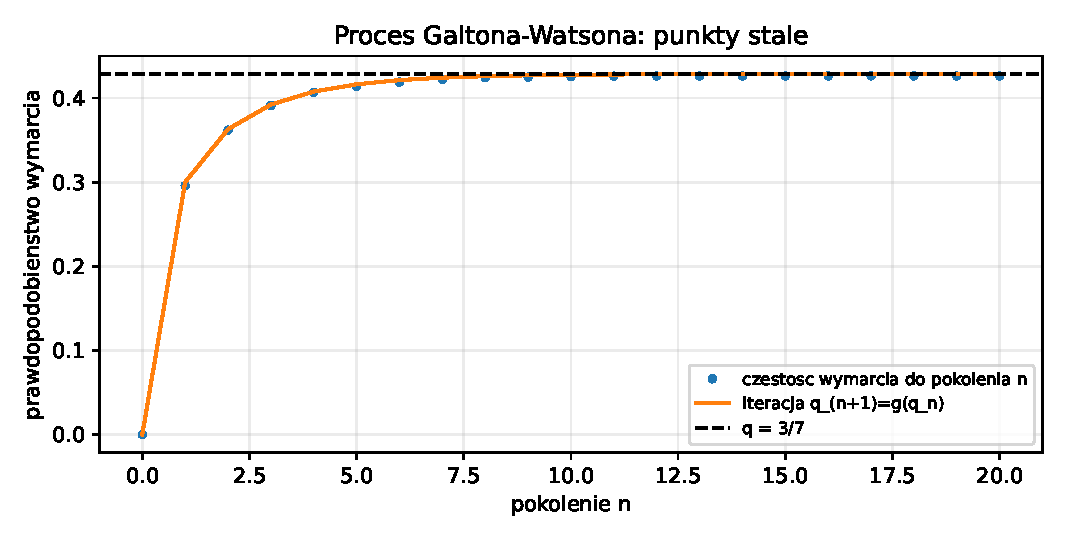
\includegraphics[width=0.88\textwidth]{figures/II_rozgalezienia.pdf}\par
\small\emph{Rysunek: Wymieranie populacji jako minimalny punkt stały funkcji tworzącej.}
\end{center}
\noindent\textbf{Kod w Pythonie (NumPy, Matplotlib).} Plik \texttt{code/II\_rozgalezienia.py} można uruchomić niezależnie; zapisuje pokazany wykres.
\lstinputlisting[language=Python]{code/II_rozgalezienia.py}
% --- KONIEC ROZSZERZENIA ILUSTRACYJNEGO ---

\section{Wariancja, normalizacja i granica martyngału}\label{sec:volII:10:04}
\begin{twierdzenie}[Wariancja pokolenia]\label{thm:volII:10:05}
Załóżmy, że $Z_0=1$, $0<m=\E\xi<\infty$ oraz
$\sigma^2=\Var(\xi)<\infty$. Wtedy
\[
\Var(Z_n)=
\begin{cases}
\displaystyle \sigma^2m^{n-1}\frac{m^n-1}{m-1},&m\ne1,\ n\ge1,\\[6pt]
 n\sigma^2,&m=1,\ n\ge0.
\end{cases}
\]
Jeżeli $m>1$, martyngał $W_n=Z_n/m^n$ jest ograniczony
w $L^2$, zatem zbiega w $L^2$ i prawie na pewno do
pewnej zmiennej $W_\infty\ge0$ o $\E W_\infty=1$ oraz
\[
\Var(W_\infty)=\frac{\sigma^2}{m(m-1)}.
\]
\end{twierdzenie}
\begin{proof}
Z niezależności potomstwa, przy warunku $Z_n=k$,
$\Var(Z_{n+1}\mid\calF_n)=\sigma^2Z_n$.
Wzór na wariancję całkowitą daje dla $v_n=\Var(Z_n)$
\[
v_{n+1}=\E[\sigma^2Z_n]
+\Var(mZ_n)=\sigma^2m^n+m^2v_n,
\quad v_0=0.
\]
Indukcja daje
$v_n=\sigma^2\sum_{j=0}^{n-1}m^{2(n-1-j)+j}
=\sigma^2m^{n-1}\sum_{j=0}^{n-1}m^j$,
co po zsumowaniu szeregu geometrycznego daje wzór.
Dla $m>1$ otrzymujemy
$\Var(W_n)=m^{-2n}v_n
=\frac{\sigma^2}{m(m-1)}(1-m^{-n})$.
Ponieważ $\E W_n=1$, drugie momenty są jednostajnie
ograniczone. Z twierdzenia o zbieżności martyngałów
ograniczonych w $L^2$ dostajemy granicę w $L^2$ i p.n.;
przejście do granicy w pierwszych i drugich momentach daje
deklarowane wzory.
\end{proof}

\begin{uwaga}[Wartość oczekiwana granicy nie zawsze zachowuje się sama]
Dla $m>1$ nieujemny martyngał $W_n$ ma granicę prawie na pewno
nawet bez założenia skończonej wariancji, ale z tego
\emph{nie wynika} automatycznie $\E W_\infty=1$.
Skończoność wariancji jest tutaj wygodnym dostatecznym
warunkiem jednostajnej całkowalności. Bardziej ogólny
warunek zachowania średniej w procesie nadkrytycznym
wiąże się z twierdzeniem Kestena--Stiguma i momentem
$\E[\xi\log^+\xi]$; ten głębszy wynik można omówić
przy bardziej zaawansowanych procesach rozgałęziających.
\end{uwaga}

\section{Całkowita liczba urodzonych osobników}\label{sec:volII:10:05}
\begin{twierdzenie}[Średnia całkowita liczba osobników]\label{thm:volII:10:06}
Niech $Z_0=1$ i $m=\E\xi<1$.
Zdefiniujmy całkowitą liczebność drzewa genealogicznego
$H=\sum_{n=0}^\infty Z_n$, gdzie suma może przyjmować $\infty$.
Wtedy $H<\infty$ prawie na pewno i
$\E H=1/(1-m)$.
\end{twierdzenie}
\begin{proof}
Zmienne $Z_n$ są nieujemne. Twierdzenie Tonellego
i wzór $\E Z_n=m^n$ dają
\[
\E H=\sum_{n=0}^\infty\E Z_n=\sum_{n=0}^\infty m^n
=\frac{1}{1-m}<\infty.
\]
Gdyby $\Prob(H=\infty)>0$, wartość oczekiwana $H$
byłaby nieskończona. Stąd $H<\infty$ prawie na pewno.
\end{proof}

\begin{stwierdzenie}[Funkcja tworząca całkowitej liczebności]\label{prop:volII:10:01}
Niech $Z_0=1$ i $\Prob(H<\infty)=1$.
Dla $s\in[0,1]$ funkcja $h(s)=\E[s^H]$ spełnia
\[
h(s)=s f(h(s)),
\]
gdzie $f$ jest funkcją tworzącą liczby potomków.
\end{stwierdzenie}
\begin{proof}
Po usunięciu pierwszego przodka drzewo rozdziela się
na $\xi$ niezależnych drzew potomków, każde o tym samym
prawie co pierwotne. Ich całkowite liczebności $H_j$
są niezależnymi kopiami $H$, niezależnymi od $\xi$.
Mamy $H=1+\sum_{j=1}^\xi H_j$.
Warunkowanie względem $\xi$ daje
$\E[s^H\mid\xi]=s\,h(s)^\xi$, skąd po uśrednieniu
$h(s)=sf(h(s))$.
\end{proof}

\begin{zadanie}[Potomstwo Poissona]
Niech liczba potomków każdego osobnika ma rozkład
$\mathrm{Poisson}(\lambda)$, $0<\lambda<1$.
Obliczyć średnią całkowitą liczebność i równanie
dla jej funkcji tworzącej.

\emph{Rozwiązanie.} Mamy
$f(s)=\exp(\lambda(s-1))$ i $m=\lambda$.
Stąd $\E H=1/(1-\lambda)$ oraz
$h(s)=s\exp(\lambda(h(s)-1))$.
To równanie pozwala numerycznie obliczać
$\Prob(H=k)$, bez budowania całego losowego drzewa.
\end{zadanie}

\section{Model rozgałęziania w czasie ciągłym: proces Yule'a}\label{sec:volII:10:06}
\begin{definicja}[Proces czystych urodzin Yule'a]\label{def:volII:10:04}
Niech $\lambda>0$. Procesem Yule'a rozpoczynającym się
od jednego osobnika nazywamy minimalny łańcuch Markowa
w czasie ciągłym na $\{1,2,3,\ldots\}$ z intensywnościami
$q_{n,n+1}=\lambda n$, $q_{nn}=-\lambda n$ oraz
$q_{n,j}=0$ dla pozostałych $j$.
Interpretacja: każdy z $n$ obecnych osobników rodzi
kolejnego niezależnie z intensywnością $\lambda$.
\end{definicja}

\begin{twierdzenie}[Brak eksplozji i rozkład geometryczny]\label{thm:volII:10:07}
Proces Yule'a rozpoczynający się od $Z_0=1$ nie wybucha
w skończonym czasie. Dla wszystkich $t\ge0$ i $n\ge1$
\[
\Prob(Z_t=n)=e^{-\lambda t}(1-e^{-\lambda t})^{n-1},
\qquad \E Z_t=e^{\lambda t}.
\]
\end{twierdzenie}
\begin{proof}
Po przejściu ze stanu $n$ proces musi przejść do $n+1$.
Czas oczekiwania w stanie $n$ ma rozkład
$\mathrm{Exp}(\lambda n)$; kolejne czasy są niezależne.
Suma $n$ pierwszych czasów oczekiwania jest czasem przejścia
od $1$ do $n+1$. Jej transformata Laplace'a dla $c>0$ to
$\prod_{k=1}^n (\lambda k)/(\lambda k+c)$.
Gdyby czas eksplozji $\zeta=\sum_{k\ge1}H_k$ był
skończony z dodatnim prawdopodobieństwem, to
$\E e^{-c\zeta}>0$. Tymczasem
$\sum_{k\ge1}\log(1+c/(\lambda k))=\infty$,
ponieważ dla dużych $k$ wyrazy są nie mniejsze od
$c/(2\lambda k)$, a szereg harmoniczny jest rozbieżny.
Zatem $\E e^{-c\zeta}=0$, co wymusza
$\Prob(\zeta=\infty)=1$. To jest bezpośredni dowód
przypadku kryterium eksplozji potrzebnego tutaj.

Dla przejść rozkładu $p_n(t)=\Prob(Z_t=n)$
uzasadnimy najpierw użycie równań w przód, chociaż przestrzeń
stanów jest nieskończona. Dla każdego ustalonego $K\ge2$
zastąpmy stany $K+1,K+2,\ldots$ jednym pochłaniającym
stanem $\partial$, nie zmieniając przejść z $1,\ldots,K$.
Do pierwszego osiągnięcia $K+1$ oba procesy są identyczne,
a ponieważ proces Yule'a wykonuje jedynie skoki $n\to n+1$,
dla $j\le K$ ich prawdopodobieństwa przebywania w stanie $j$
są równe. Proces obcięty ma skończoną przestrzeń stanów;
możemy więc zastosować wcześniej udowodnione równania
Kołmogorowa w przód, a otrzymane równania dla $p_j$, $j\le K$,
nie zależą od $K$. Dowodzi to dla wszystkich $n\ge1$ równań
$p_1'(t)=-\lambda p_1(t)$,
$p_n'(t)=-n\lambda p_n(t)+(n-1)\lambda p_{n-1}(t)$ dla $n\ge2$,
z warunkami $p_1(0)=1$ i $p_n(0)=0$ dla $n\ge2$.
Pierwsze równanie daje $p_1(t)=e^{-\lambda t}$.
Podstawiając kandydat
$p_n(t)=a(t)(1-a(t))^{n-1}$, gdzie $a(t)=e^{-\lambda t}$,
i korzystając z $a'=-\lambda a$, otrzymujemy po różniczkowaniu
$p_n'=-\lambda a(1-a)^{n-1}+\lambda(n-1)a^2(1-a)^{n-2}$.
Prawa strona równania Kołmogorowa wynosi
$-n\lambda a(1-a)^{n-1}+(n-1)\lambda a(1-a)^{n-2}$,
co po wyłączeniu $\lambda a(1-a)^{n-2}$ sprowadza się do
$-n(1-a)+(n-1)=na-1$,
tak samo jak pierwsza pochodna.
Jednoznaczność rozwiązań wynika indukcyjnie: każde równanie
jest liniowym równaniem niejednorodnym z wcześniej znaną
funkcją $p_{n-1}$. Ponieważ kandydat daje rozkład
prawdopodobieństwa ($\sum_{n\ge1}a(1-a)^{n-1}=1$),
odzyskujemy prawo procesu. Średnia rozkładu
geometrycznego na $\{1,2,\ldots\}$ wynosi $1/a=e^{\lambda t}$.
\end{proof}

\begin{uwaga}[Dwa odmienne mechanizmy wzrostu]
W procesie Galtona--Watsona wszyscy osobnicy rozmnażają się
w kolejnych \emph{pokoleniach}, a liczebność zmienia się
skokowo w chwilach całkowitych. W procesie Yule'a
urodzenia pojawiają się w \emph{czasie ciągłym}, przy czym
intensywność łączna rośnie proporcjonalnie do bieżącej liczby
osobników. Oba procesy mają strukturę rozgałęziającą,
ale inne trajektorie, rozkłady i narzędzia obliczeniowe.
\end{uwaga}


\section{Jak szybko zanika prawdopodobieństwo przetrwania?}\label{sec:volII:10:07}
\begin{stwierdzenie}[Ogon czasu wymarcia w przypadku podkrytycznym]\label{prop:volII:10:02}
Niech $Z$ będzie procesem Galtona--Watsona rozpoczynającym się
od $Z_0=1$ ze średnią potomstwa $m\in[0,1)$.
Niech $\tau=\inf\{n\ge0:Z_n=0\}$.
Wtedy dla każdego $n\ge0$
\[
\Prob(\tau>n)=\Prob(Z_n>0)\le m^n,
\qquad \E\tau\le\frac{1}{1-m}.
\]
\end{stwierdzenie}
\begin{proof}
Ponieważ zero jest stanem pochłaniającym,
$\{\tau>n\}=\{Z_n>0\}$. Dla nieujemnej zmiennej
całkowitoliczbowej nierówność Markowa daje
$\Prob(Z_n>0)=\Prob(Z_n\ge1)\le\E Z_n=m^n$.
Wzór ogonowy dla zmiennej o wartościach w $\N_0\cup\{\infty\}$,
wynikający z twierdzenia Tonellego, ma postać
$\E\tau=\sum_{n=0}^\infty\Prob(\tau>n)$.
Sumując oszacowania, otrzymujemy deklarowaną granicę.
\end{proof}

\begin{uwaga}[Dlaczego przypadek krytyczny wymaga innej metody?]
Jeżeli $m=1$ i $p_0>0$, populacja wymiera prawie na pewno,
ale oszacowanie $\Prob(Z_n>0)\le m^n=1$ niczego nie mówi
o szybkości wymierania. W typowym przypadku krytycznym
ze skończoną dodatnią wariancją potomstwa prawdopodobieństwo
przetrwania maleje tylko jak stała podzielona przez $n$.
Dokładna asymptotyka jest osobnym twierdzeniem granicznym;
nie wynika z samego argumentu o punktach stałych.
\end{uwaga}

\section{Urodzenia i śmierci w czasie ciągłym}\label{sec:volII:10:08}
\begin{twierdzenie}[Prawdopodobieństwo wymarcia liniowego procesu urodzin i śmierci]\label{thm:volII:10:08}
Niech $\lambda,\delta>0$. Rozważmy minimalny łańcuch Markowa
$Z$ na $\N_0$, rozpoczynający się od $Z_0=1$, z intensywnościami
$q_{n,n+1}=\lambda n$, $q_{n,n-1}=\delta n$ dla $n\ge1$,
$q_{nn}=-(\lambda+\delta)n$, zaś $0$ jest stanem pochłaniającym.
Wtedy proces jest nieeksplozywny, a prawdopodobieństwo
ostatecznego wymarcia wynosi
\[
q=\begin{cases}1,&\lambda\le\delta,\\
\delta/\lambda,&\lambda>\delta.
\end{cases}
\]
\end{twierdzenie}
\begin{proof}
Najpierw uzasadnimy brak eksplozji bez odwoływania się do
nieformalnego sprzężenia. Dla $K\ge2$ niech
$\tau_K=\inf\{t\ge0:Z_t\ge K\}$. Proces zatrzymany
$Z_{t\wedge\tau_K}$ przyjmuje wartości w skończonym
zbiorze $\{0,1,\ldots,K\}$. Dla funkcji $f(n)=n$
jego generator przed zatrzymaniem wynosi
$Qf(n)=(\lambda-\delta)n\le\lambda n$.
Wzór Dynkina dla skończonego, zatrzymanego łańcucha
daje dla $u_K(t)=\E Z_{t\wedge\tau_K}$
\[
u_K(t)\le1+\lambda\int_0^tu_K(s)\,\dd s.
\]
Nierówność Gronwalla prowadzi do
$u_K(t)\le e^{\lambda t}$. Ponieważ
$Z_{t\wedge\tau_K}=K$ na $\{\tau_K\le t\}$,
$\Prob(\tau_K\le t)\le e^{\lambda t}/K$.
Każdy skok zmienia liczbę osobników o jeden, zatem
eksplozja w skończonym czasie wymaga osiągnięcia
każdego poziomu $K$. Dla każdego $t<\infty$
$\Prob(\zeta\le t)\le\inf_{K\ge2}e^{\lambda t}/K=0$,
gdzie $\zeta$ oznacza czas eksplozji. Proces jest zatem
nieeksplozywny.

Rozważmy pierwsze zdarzenie po starcie od jednego osobnika.
Łączna intensywność wynosi $\lambda+\delta$, a jego rodzaj
jest niezależny od czasu oczekiwania: z prawdopodobieństwem
$\delta/(\lambda+\delta)$ osobnik umiera, z prawdopodobieństwem
$\lambda/(\lambda+\delta)$ rodzi drugiego osobnika.
Po urodzeniu mamy dwa niezależne drzewa potomne, każde
o takim samym prawdopodobieństwie wymarcia $q$.
Wobec tego
\[
q=\frac{\delta}{\lambda+\delta}
+\frac{\lambda}{\lambda+\delta}q^2.
\]
Rozwiązaniami są $1$ i $\delta/\lambda$.
Uzasadnijmy wybór mniejszego pierwiastka. Każdy żyjący
osobnik ma niezależny czas do pierwszego zdarzenia
o rozkładzie $\mathrm{Exp}(\lambda+\delta)$; wtedy
z prawdopodobieństwem $\delta/(\lambda+\delta)$
umiera bez potomków, a z prawdopodobieństwem
$\lambda/(\lambda+\delta)$ rodzi nowego osobnika.
W drugim przypadku można potraktować dotychczasowego
osobnika (z uwagi na własność braku pamięci) i nowego
jako \emph{dwie niezależne linie potomne}. Drzewo
zdarzeń jest więc drzewem Galtona--Watsona z liczbą
dzieci $0$ lub $2$ i funkcją tworzącą
$f(s)=\delta/(\lambda+\delta)+\lambda s^2/(\lambda+\delta)$.
Zdarzenie, że drzewo ma skończoną liczbę węzłów,
jest sumą zdarzeń wymarcia do skończonej głębokości;
jego prawdopodobieństwo jest zatem granicą iteracji
$f^{\circ n}(0)$, czyli najmniejszym punktem stałym $f$.
Jeżeli drzewo jest skończone, wszystkie związane z nim
czasy oczekiwania są skończone prawie na pewno,
a więc proces rzeczywiście osiąga stan $0$ w skończonym
czasie. Odwrotnie, jeśli osiąga $0$ w skończonym czasie,
to brak eksplozji oznacza skończoną liczbę zdarzeń do tej
chwili, a zatem skończone drzewo genealogiczne.
Wymarcie procesu jest więc dokładnie wymarciem tego drzewa.
Stosując kryterium z wcześniejszej części rozdziału,
wybieramy najmniejszy pierwiastek: $q=1$ przy
$\lambda\le\delta$ i $q=\delta/\lambda$ przy
$\lambda>\delta$.
\end{proof}

\begin{zadanie}[Próg przeżycia populacji]
Niech każda żyjąca cząstka rodzi nową z intensywnością
$\lambda=3$ i ginie z intensywnością $\delta=2$,
niezależnie od pozostałych. Rozpoczynamy od jednej cząstki.
Jakie jest prawdopodobieństwo, że populacja kiedyś wymrze?

\emph{Rozwiązanie.} Pierwsze zdarzenie jest śmiercią
z prawdopodobieństwem $2/5$ lub narodzinami z prawdopodobieństwem
$3/5$. Stąd $q=2/5+(3/5)q^2$, więc
$(3q-2)(q-1)=0$.
Wybieramy mniejsze rozwiązanie: $q=2/3$.
Średni dodatni przyrost liczby osobników nie gwarantuje
przetrwania konkretnego drzewa genealogicznego.
\end{zadanie}


\begin{zadanie}[Wzrost procesu Yule'a]
Niech $Z$ będzie procesem Yule'a o intensywności $\lambda>0$
z jednym osobnikiem początkowym. Wyznaczyć
$\Prob(Z_t\ge k)$, $\Var(Z_t)$ i
$\Prob(Z_t\ge3\mid Z_t\ge2)$ dla $t>0$, $k\ge1$.

\emph{Rozwiązanie.} Wprowadzamy $a=e^{-\lambda t}$.
Z udowodnionego wzoru $\Prob(Z_t=n)=a(1-a)^{n-1}$
otrzymujemy przez zsumowanie szeregu geometrycznego
$\Prob(Z_t\ge k)=(1-a)^{k-1}$.
Dla rozkładu geometrycznego na $\{1,2,\dots\}$
$\E Z_t=1/a$ i $\Var(Z_t)=(1-a)/a^2$, a więc
$\Var(Z_t)=e^{2\lambda t}-e^{\lambda t}$.
Wreszcie
\[
\Prob(Z_t\ge3\mid Z_t\ge2)
=\frac{(1-a)^2}{1-a}=1-e^{-\lambda t}.
\]
To przykład odrębnej własności braku pamięci
\emph{rozkładu geometrycznego liczebności},
a nie wykładniczego rozkładu czasów między skokami.
\end{zadanie}

\section{Podsumowanie i kierunek dalszej teorii}\label{sec:volII:10:09}
Łańcuch Markowa opisuje przejścia między stanami;
proces odnowy opisuje cykle; proces rozgałęziający
opisuje losową liczbę \emph{potomków}, którzy sami
stają się źródłem kolejnych losowań. Funkcje tworzące
zamieniają złożoną strukturę drzew na iterację funkcji,
a martyngały pozwalają śledzić zmienność populacji
w kolejnych pokoleniach. Dalszym krokiem będą martyngały w czasie ciągłym, lokalizacja,
zatrzymywanie i wariacja kwadratowa. Całka Itô i równania
stochastyczne zostaną skonstruowane dopiero w tomie III.


% ================================================================
% ROZDZIAŁ 11. MARTYNGAŁY W CZASIE CIĄGŁYM
% ================================================================
\chapter{Martyngały w czasie ciągłym: informacja, regularność i lokalizacja}
\label{chap:volII:11}
\par\smallskip\noindent{\small\textit{Powiązania:} \textup{tom~I}, sekcja~\ref{I-sec:volI:14:01} (martyngały dyskretne); \textup{tom~I}, sekcja~\ref{I-sec:volI:15:03} (zbieżność martyngałów); \textup{tom~III}, sekcja~\ref{III-sec:volIII:02:01} (konstrukcja całki Itô); tom~I, twierdzenie~\ref{I-thm:volI:15:03} (twierdzenie Dooba o zbieżności).}\par\smallskip

\label{ch:mart-cont}

\section{Dlaczego przejście od czasu dyskretnego nie jest automatyczne?}\label{sec:volII:11:01}
W tomie I martyngał był ciągiem $(M_n)_{n\ge0}$, którego
warunkowa prognoza następnej wartości, przy znajomości przeszłości,
wynosiła dokładnie wartość obecną. W czasie ciągłym rozważamy
nieprzeliczalną rodzinę chwil. Pojawiają się dwa nowe pytania:
jak wybierać jedną wspólną wersję trajektorii oraz co znaczy
zatrzymać proces w chwili wybranej na podstawie obserwacji?
Później zobaczymy też, że proces ze skokami może być martyngałem,
mimo że jego trajektorie mają skończoną wariację całkowitą.

\begin{definicja}[Martyngał, podmartyngał i nadmartyngał]\label{def:volII:11:01}
Niech $(\Omega,\calF,\Prob)$ będzie przestrzenią probabilistyczną,
$(\calF_t)_{t\ge0}$ filtracją i $M=(M_t)_{t\ge0}$ procesem
rzeczywistym, adaptowanym, takim że $\E|M_t|<\infty$
dla każdego $t\ge0$. Proces $M$ jest \emph{martyngałem}, jeśli
$\E[M_t\mid\calF_s]=M_s$ prawie na pewno dla wszystkich
$0\le s\le t$. Jest \emph{podmartyngałem}, jeśli
$\E[M_t\mid\calF_s]\ge M_s$, a \emph{nadmartyngałem},
gdy zachodzi nierówność przeciwna. Filtracja spełnia
\emph{warunki zwykłe}, jeśli jest zupełna (każdy podzbiór zbioru z $\calF$ o prawdopodobieństwie
zero należy do $\calF_0$) i prawostronnie ciągła:
$\calF_t=\bigcap_{u>t}\calF_u$ dla każdego $t\ge0$.
\end{definicja}

Ważne, że równość dla każdej pary $s,t$ jest rozumiana osobno
prawie na pewno. Nie wolno bez dodatkowego argumentu zażądać
jednego zbioru miary jeden, na którym równości warunkowe
miałyby zachodzić jednocześnie dla nieprzeliczalnie wielu par.

\begin{przyklad}[Trzy modele uczciwej ewolucji]
Niech $W$ będzie standardowym procesem Wienera w jego
uzupełnionej filtracji naturalnej. Wówczas
$W_t$ jest martyngałem z powodu niezależnych wycentrowanych
przyrostów. Proces $W_t^2-t$ również nim jest, ponieważ
\[
\E[W_t^2-t\mid\calF_s]
=W_s^2+\E[(W_t-W_s)^2]-t=W_s^2-s.
\]
Jeśli $N$ jest procesem Poissona o intensywności $\lambda>0$,
to $N_t-\lambda t$ jest martyngałem, gdyż przyrost liczby
zdarzeń po chwili $s$ jest niezależny od przeszłości i ma
średnią $\lambda(t-s)$. Pierwsze dwa procesy mają trajektorie
ciągłe, ostatni ma skoki wysokości jeden.
\end{przyklad}

\begin{lemat}[Warunkowe wartości oczekiwane są jednostajnie całkowalne]\label{lem:volII:11:01}
Niech $X\in L^1(\Omega,\calF,\Prob)$. Rodzina
$\{\E[X\mid\calG]:\calG\subseteq\calF\text{ jest pod-}\sigma\text{-ciałem}\}$
jest jednostajnie całkowalna.
\end{lemat}
\begin{proof}
Ustalmy $K>0$ i rozłóżmy $X=U+V$, gdzie
$U=X\ind{\{|X|\le K/2\}}$ oraz
$V=X\ind{\{|X|>K/2\}}$. Dla dowolnego $\calG$
połóżmy $Y=\E[X\mid\calG]$. Wówczas
$|\E[U\mid\calG]|\le K/2$, skąd na zdarzeniu
$\{|Y|>K\}$ zachodzi $|\E[V\mid\calG]|>K/2$
i $|Y|\le K/2+|\E[V\mid\calG]|\le2|\E[V\mid\calG]|$.
Dlatego
\[
\E[|Y|\ind{\{|Y|>K\}}]
\le2\E|\E[V\mid\calG]|
\le2\E|V|
=2\E[|X|\ind{\{|X|>K/2\}}].
\]
Prawa strona nie zależy od $\calG$ i dąży do zera
przy $K\to\infty$ dzięki całkowalności $X$.
\end{proof}

\begin{wniosek}[Jednostajna całkowalność na skończonym horyzoncie]\label{cor:volII:11:01}
Niech $M$ będzie martyngałem oraz $T<\infty$.
Wtedy rodzina $\{M_t:0\le t\le T\}$ jest jednostajnie
całkowalna, gdyż $M_t=\E[M_T\mid\calF_t]$.
\end{wniosek}

\section{Prawostronne modyfikacje: skąd bierze się regularność?}\label{sec:volII:11:02}
\begin{definicja}[Trajektoria c\`adl\`ag]\label{def:volII:11:02}
Funkcja $f:[0,\infty)\to\R$ jest c\`adl\`ag, jeśli
jest prawostronnie ciągła i ma skończone granice lewostronne
we wszystkich chwilach $t>0$. Proces jest c\`adl\`ag,
gdy prawie wszystkie jego trajektorie mają tę własność.
\end{definicja}

\begin{lemat}[Zbieżność odwrotnych warunkowych wartości oczekiwanych]\label{lem:volII:11:02}
Niech $(\calG_n)_{n\ge1}$ będzie malejącym ciągiem
pod-$\sigma$-ciał przestrzeni $(\Omega,\calF,\Prob)$,
$\calG_\infty=\bigcap_n\calG_n$, a $X\in L^1$.
Wtedy
$\E[X\mid\calG_n]\to\E[X\mid\calG_\infty]$ w $L^1$.
\end{lemat}
\begin{proof}
Najpierw niech $X\in L^2$ i $Y_n=\E[X\mid\calG_n]$.
Dla $m\ge n$ mamy $Y_m=\E[Y_n\mid\calG_m]$.
Ortogonalność rzutu warunkowego daje
$\|Y_n-Y_m\|_2^2=\|Y_n\|_2^2-\|Y_m\|_2^2$.
Normy $\|Y_n\|_2$ maleją i są nieujemne, zatem
$(Y_n)$ jest ciągiem Cauchy'ego w $L^2$. Niech $Y$
będzie jego granicą. Dla każdego ustalonego $k$ wszystkie
$Y_n$ z $n\ge k$ są $\calG_k$-mierzalne; domkniętość
$L^2(\calG_k)$ daje mierzalność $Y$ względem każdego
$\calG_k$, czyli względem $\calG_\infty$.
Dla $A\in\calG_\infty$ i wszystkich $n$ mamy
$\E[Y_n\ind A]=\E[X\ind A]$; przejście do granicy
w $L^1$ identyfikuje $Y=\E[X\mid\calG_\infty]$.
Dla ogólnego $X\in L^1$ przybliżamy $X$ obcięciami
$X^{(K)}\in L^2$. Kontrakcja warunkowania w $L^1$
pozwala przenieść zbieżność z $X^{(K)}$ na $X$ po
przejściu $K\to\infty$.
\end{proof}

\begin{lemat}[Dlaczego z ograniczonej liczby przekroczeń wynikają granice?]\label{lem:volII:11:03}
Niech $D$ będzie gęstym podzbiorem przedziału $[0,T]$,
a $f:D\to\R$ funkcją ograniczoną. Załóżmy, że dla każdej
pary liczb wymiernych $a<b$ funkcja $f$, oglądana w
rosnącym porządku chwil z $D$, ma skończenie wiele pełnych
przekroczeń przedziału $[a,b]$ w górę. Wtedy w każdej chwili
$t<T$ istnieje skończona prawa granica
$\lim_{r\downarrow t,\,r\in D}f(r)$, a w każdej chwili
$t>0$ istnieje skończona lewa granica wzdłuż $D$.
Funkcja zdefiniowana przez prawe granice (z wartością $f(T)$
w końcu przedziału, gdy $T\in D$) jest c\`adl\`ag.
\end{lemat}
\begin{proof}
Brak prawej granicy w chwili $t$ oznaczałby
$\liminf_{r\downarrow t,\,r\in D}f(r)
<\limsup_{r\downarrow t,\,r\in D}f(r)$.
Można wtedy wybrać wymierne $a<b$ pomiędzy tymi
liczbami oraz dowolnie długie skończone ciągi chwil
z $D\cap(t,t+\delta)$, w których wartości naprzemiennie
spadają poniżej $a$ i rosną powyżej $b$.
Po ustawieniu chwil rosnąco otrzymujemy dowolnie wiele
przekroczeń w górę, sprzecznie z założeniem.
To samo rozumowanie, z chwilami zbliżającymi się do $t$
od lewej, daje istnienie granicy lewostronnej.
Ograniczoność $f$ zapewnia skończoność obu granic.

Oznaczmy prawą granicę przez $g(t)$. Gdyby dla
$t_n\downarrow t$ zachodziło $g(t_n)\not\to g(t)$,
można by znaleźć $r_n\in D$ położone tuż za $t_n$,
tak by $r_n\downarrow t$ oraz
$|f(r_n)-g(t_n)|\to0$; byłaby to sprzeczność z
definicją $g(t)$. Analogicznie, dla $t_n\uparrow t$
wybieramy $r_n\in D$ między $t_n$ i $t$.
Istnienie lewej granicy $f$ w $t$ pociąga wówczas
istnienie tej samej lewej granicy dla $g$.
Zatem $g$ jest prawostronnie ciągła i ma granice
lewostronne.
\end{proof}

\begin{twierdzenie}[Regularizacja martyngału typu zamkniętego]\label{thm:volII:11:01}
\label{thm:regularizacja}
Niech filtracja $(\calF_t)_{t\ge0}$ spełnia warunki zwykłe,
a $X\in L^1(\Omega,\calF,\Prob)$. Proces
$M_t=\E[X\mid\calF_t]$ ma modyfikację c\`adl\`ag.
Dokładniej, istnieje proces $\widetilde M$ o trajektoriach
c\`adl\`ag, taki że dla każdego $t\ge0$
$\widetilde M_t=M_t$ prawie na pewno.
\end{twierdzenie}
\begin{proof}
Ustalmy skończony horyzont $T>0$ i wybierzmy
$D_T=(\Q\cap[0,T])\cup\{T\}$. Dla dowolnych liczb
wymiernych $a<b$ i skończonego uporządkowanego podzbioru
$D_T$ zastosujmy nierówność przekroczeń do dyskretnego
martyngału otrzymanego przez próbkowanie $(M_t)$ w tych
chwilach. Oczekiwana liczba przekroczeń przedziału
$[a,b]$ jest ograniczona przez stałą zależną od
$a,b$ i $\E|X|$, a nie od liczby punktów próbkowania:
taki wniosek wynika z dowodu nierówności przekroczeń
zamieszczonego w tomie I (i ponownie w rozdziale
\ref{ch:stop-cont}). Przechodząc po rosnących skończonych
podzbiorach do całego $D_T$, otrzymujemy prawie na pewno
skończoną liczbę przekroczeń każdego przedziału
wymiernego. Wynika stąd istnienie skończonych granic
jednostronnych $M_{s-}$ i $M_{s+}$ wzdłuż $D_T$
we wszystkich chwilach $s\in(0,T)$, z wyjątkiem jednego
zbioru zerowego (zastosowaliśmy tylko przeliczalnie wiele
par $a<b$). Skończoność granic wynika też z ograniczenia
$\sup_{r\in D_T}|M_r|<\infty$ prawie na pewno;
to ostatnie uzyskujemy z nierówności maksymalnej w $L^1$
dla skończonych podzbiorów i zbieżności monotonicznej.

Definiujemy $\widetilde M_s=\lim_{r\downarrow s,r\in D_T}M_r$
dla $s<T$ oraz $\widetilde M_T=M_T$. Poprzedni lemat
o funkcjach rzeczywistych z granicami jednostronnymi
zapewnia, że $s\mapsto\widetilde M_s$ jest prawostronnie
ciągła i ma granice z lewej: gdyby prawostronna ciągłość
zawiodła, powstałyby dwie sekwencje punktów zbieżne do
tej samej chwili o różnych granicach, sprzeczne z istnieniem
wspólnej granicy prawostronnej próbek z $D_T$.

Aby sprawdzić, że to modyfikacja właściwego procesu, dla
każdego ustalonego $s<T$ wybieramy $r_n\in D_T$ malejące
do $s$. Z lematu o malejących $\sigma$-ciałach i prawostronnej
ciągłości filtracji
$M_{r_n}=\E[X\mid\calF_{r_n}]\to
\E[X\mid\calF_s]=M_s$ w $L^1$.
Z drugiej strony lewa strona zbiega prawie na pewno do
$\widetilde M_s$. Stąd $\widetilde M_s=M_s$ prawie na pewno.
Łącząc konstrukcje na horyzontach $T=1,2,\ldots$
(na wspólnym zbiorze pełnej miary), otrzymujemy proces
na $[0,\infty)$; wartości na nakładających się odcinkach
są zgodne jako prawe granice z tego samego zbioru
wymiernych chwil.
\end{proof}

\begin{uwaga}[Dlaczego wymagana jest prawostronna ciągłość filtracji?]
Bez warunku $\calF_{t+}=\calF_t$ granica
$\E[X\mid\calF_r]$ przy $r\downarrow t$ może być
warunkową wartością względem większego $\sigma$-ciała
$\calF_{t+}$, a nie względem $\calF_t$.
Uzyskujemy wtedy proces prawostronnie ciągły, który w chwili
$t$ może wykorzystywać informację niedostępną w $\calF_t$.
To jest powód, dla którego warunki zwykłe są podstawowym
założeniem teorii w czasie ciągłym.
\end{uwaga}


\begin{przyklad}[Dlaczego nie wystarcza lewostronna informacja?]
Niech $\Omega=\{-1,1\}$, obydwa wyniki mają prawdopodobieństwo
$1/2$, a $X(\omega)=\omega$. Przyjmijmy $\calF_0=\{\varnothing,\Omega\}$
oraz $\calF_t=\sigma(X)$ dla $t>0$. Wtedy
$M_t=\E[X\mid\calF_t]$ ma postać $M_0=0$ i $M_t=X$ dla $t>0$.
Jest to martyngał, ale nie posiada modyfikacji prawostronnie ciągłej
w chwili zero. Istotnie, dla wszystkich wymiernych $r>0$
każda modyfikacja musiałaby mieć $\widetilde M_r=X$ poza jednym
wspólnym zbiorem zerowym, a więc prawa granica w zerze wynosiłaby
$X\ne0=\widetilde M_0$ prawie na pewno. Filtracja nie jest
prawostronnie ciągła w zerze, ponieważ
$\calF_{0+}=\bigcap_{t>0}\calF_t=\sigma(X)\supsetneq\calF_0$.
Ten przykład ujawnia, że regularizacja jest twierdzeniem o
\emph{procesie oraz informacji}, a nie wyłącznie o funkcjach czasu.
\end{przyklad}

\begin{lemat}[Mierzalność wartości procesu zatrzymanego]\label{lem:volII:11:04}
Niech $X=(X_t)_{t\ge0}$ będzie rzeczywistym procesem adaptowanym
o wszędzie prawostronnie ciągłych trajektoriach, a $\tau$ czasem zatrzymania.
Dla każdego $t\ge0$ zmienna $X_{t\wedge\tau}$ jest $\calF_t$-mierzalna.
\end{lemat}
\begin{proof}
Ustalmy $t>0$. Przybliżamy $\tau\wedge t$ od góry przez czasy
$\rho_n=2^{-n}\lceil2^n(\tau\wedge t)\rceil\wedge t$, które
przyjmują skończenie wiele wartości z $[0,t]$ i są czasami
zatrzymania. Dla każdego $n$ mamy
$X_{\rho_n}=\sum_{u\in D_n}X_u\ind{\{\rho_n=u\}}$,
gdzie $D_n$ jest skończonym zbiorem wartości $\rho_n$.
Każdy składnik jest $\calF_t$-mierzalny (ponieważ $u\le t$),
a $\rho_n\downarrow\tau\wedge t$. Prawostronna ciągłość daje
$X_{\rho_n}\to X_{\tau\wedge t}$ prawie na pewno, a więc ostatnia
zmienna jest mierzalna względem $\calF_t$, po ewentualnym
uzupełnieniu filtracji. Dla procesu o prawostronnie ciągłych
trajektoriach dla każdego $\omega$ argument jest punktowy.
\end{proof}


\section{Czasy zatrzymania i proces zatrzymany}\label{sec:volII:11:03}
\begin{definicja}[Proces zatrzymany]\label{def:volII:11:03}
Niech $X$ będzie procesem adaptowanym c\`adl\`ag,
a $\tau$ czasem zatrzymania (dopuszczamy wartość $\infty$).
Dla $t\ge0$ definiujemy $X_t^\tau=X_{t\wedge\tau}$.
Gdy $\tau=\infty$, przyjmujemy $t\wedge\tau=t$.
\end{definicja}

\begin{twierdzenie}[Zatrzymanie w ustalonej chwili]\label{thm:volII:11:02}
Niech $M$ będzie martyngałem c\`adl\`ag, a $\tau$
czasem zatrzymania. Wtedy $M^\tau$ jest martyngałem.
Jeżeli $X$ jest podmartyngałem (odpowiednio nadmartyngałem)
c\`adl\`ag \emph{klasy $(DL)$}, to $X^\tau$ pozostaje
podmartyngałem (odpowiednio nadmartyngałem).
Tutaj klasa $(DL)$ oznacza, że dla każdego $T<\infty$
rodzina $\{X_\sigma: \sigma\le T,\ \sigma
\text{ jest czasem zatrzymania}\}$ jest jednostajnie
całkowalna.
\end{twierdzenie}
\begin{proof}
Ustalmy $0\le s\le t$ i czas
$\rho=s\vee(t\wedge\tau)$. Ponieważ
$s\le\rho\le t$, twierdzenie o ograniczonym
próbkowaniu opcjonalnym daje
$\E[M_\rho\mid\calF_s]=M_s$.
Na zdarzeniu $\{\tau>s\}\in\calF_s$ mamy
$\rho=t\wedge\tau$, a na $\{\tau\le s\}$
proces zatrzymany jest już stały. Dlatego
\[
\begin{aligned}
\E[M_{t\wedge\tau}\mid\calF_s]
&=\ind{\{\tau\le s\}}M_\tau
 +\ind{\{\tau>s\}}\E[M_\rho\mid\calF_s]\\
&=M_{s\wedge\tau}.
\end{aligned}
\]
Dla podmartyngału $X$ klasy $(DL)$ te same przybliżenia
siatkowe czasów $s$ i $t\wedge\tau$, użyte w dowodzie
twierdzenia~\ref{thm:optional-cont}, dają
$\E[X_{t\wedge\tau}\mid\calF_s]\ge X_{s\wedge\tau}$.
Istotne jest przejście do granicy w $L^1$:
z klasy $(DL)$ otrzymujemy jednostajną całkowalność
wartości w przybliżających czasach zatrzymania,
a prawostronna ciągłość daje ich zbieżność prawie na pewno.
Nierówność przechodzi więc do granicy w warunkowych
wartościach oczekiwanych. Dla nadmartyngału zmieniamy
znak procesu i powtarzamy argument. Samo formalne
podstawienie losowej chwili w definicji podmartyngału
nie jest dowodem.
\end{proof}

\begin{uwaga}[Nie mylić zatrzymania z granicą $M_\tau$]
Powyższe twierdzenie dotyczy procesu $M_{t\wedge\tau}$
przy każdym skończonym $t$. Nie wolno z niego wnioskować
$\E M_\tau=\E M_0$ dla nieograniczonego czasu $\tau$:
przejście $t\to\infty$ wymaga dodatkowego warunku
jednostajnej całkowalności.
\end{uwaga}

\begin{zadanie}[Co odróżnia martyngał od procesu o niemalejącej średniej?]
Niech $W$ będzie standardowym procesem Wienera w jego
filtracji naturalnej. Sprawdzić bez rachunku It\^o, które
z procesów $W_t$, $W_t^2$ i $W_t^2-t$ są martyngałami.

\emph{Rozwiązanie.} Dla $s<t$ zapiszmy
$W_t=W_s+U$, gdzie $U\sim\Normal(0,t-s)$
i $U$ jest niezależne od $\calF_s$.
Stąd $\E[W_t\mid\calF_s]=W_s$.
Po podniesieniu do kwadratu i warunkowaniu otrzymujemy
\[
\E[W_t^2\mid\calF_s]
=W_s^2+2W_s\E U+\E U^2=W_s^2+(t-s).
\]
Proces $W_t^2$ jest zatem podmartyngałem, ale nie
martyngałem. Odejmując od niego deterministyczny
proces $t$, dostajemy
$\E[W_t^2-t\mid\calF_s]=W_s^2-s$.
Wyraz $t$ jest dokładnie kompensacją narastającej
wariancji, którą w kolejnym rozdziale opiszemy za
pomocą nawiasu procesu.
\end{zadanie}

\section{Martyngały lokalne}\label{sec:volII:11:04}
\begin{definicja}[Lokalny martyngał i lokalizacja]\label{def:volII:11:04}
Niech $M$ będzie adaptowanym procesem c\`adl\`ag o
wartościach rzeczywistych. Nazywamy go \emph{lokalnym
martyngałem}, jeżeli istnieją czasy zatrzymania
$\tau_k\uparrow\infty$ prawie na pewno, takie że dla
każdego $k$ proces $M^{\tau_k}$ jest martyngałem.
Ciąg $(\tau_k)$ nazywamy \emph{ciągiem lokalizującym}.
\end{definicja}

\begin{twierdzenie}[Zatrzymanie ograniczonego procesu lokalnego]\label{thm:volII:11:03}
Niech $M$ będzie ciągłym lokalnym martyngałem z $M_0=0$,
a $\tau_K=\inf\{t\ge0:|M_t|\ge K\}$ dla $K>0$.
Wówczas $M^{\tau_K}$ jest martyngałem ograniczonym
przez $K$. Czasy $\tau_K\uparrow\infty$ prawie na pewno,
gdy $K\to\infty$.
\end{twierdzenie}
\begin{proof}
Niech $\sigma_n$ lokalizuje $M$. Proces
$M^{\tau_K\wedge\sigma_n}$ jest martyngałem na mocy
próbkowania opcjonalnego zastosowanego do
$M^{\sigma_n}$: zatrzymujemy go dodatkowo w $\tau_K$.
Ciągłość $M$ daje $|M_{t\wedge\tau_K\wedge\sigma_n}|\le K$.
Dla ustalonego $t$ mamy
$M_{t\wedge\tau_K\wedge\sigma_n}\to M_{t\wedge\tau_K}$
prawie na pewno, a wspólne ograniczenie przez $K$
pozwala przejść do granicy w $L^1$.
Dla $s\le t$ przechodzimy do granicy w warunkowych
równościach martyngałowych, używając kontrakcji warunkowania
w $L^1$. Otrzymujemy martyngał $M^{\tau_K}$.
Na każdym ograniczonym przedziale trajektoria ciągła jest
ograniczona, więc dla dużego $K$ nie przekracza poziomu
$K$ na tym przedziale. To dowodzi $\tau_K\uparrow\infty$.
\end{proof}

\begin{zadanie}[Kompensowany proces Poissona i momenty]
Niech $N$ będzie procesem Poissona o intensywności
$\lambda>0$ oraz $M_t=N_t-\lambda t$. Wykazać,
że $M$ jest martyngałem, i wyznaczyć jego wariancję.

\emph{Rozwiązanie.} Dla $s<t$ przyrost
$N_t-N_s$ ma rozkład Poissona z parametrem
$\lambda(t-s)$ i jest niezależny od $\calF_s$.
Stąd $\E[M_t-M_s\mid\calF_s]=0$. Ponadto
$\Var(M_t)=\Var(N_t)=\lambda t$.
W przeciwieństwie do $W_t$, trajektoria $M$ jest
odcinkami liniowa i ma skoki wielkości $1$.
\end{zadanie}


\begin{twierdzenie}[Nieujemny lokalny martyngał jest nadmartyngałem]\label{thm:volII:11:04}
\label{thm:positive-local-supermart}
Niech $M=(M_t)_{t\ge0}$ będzie rzeczywistym lokalnym
martyngałem c\`adl\`ag względem filtracji $(\calF_t)$,
$M_t\ge0$ dla każdego $t$ poza jednym zbiorem zerowym,
oraz $\E M_0<\infty$. Wówczas $M_t\in L^1$ dla wszystkich $t$
i dla $0\le s\le t$ zachodzi
$\E[M_t\mid\calF_s]\le M_s$ prawie na pewno.
W szczególności $\E M_t\le\E M_0$.
\end{twierdzenie}
\begin{proof}
Niech $(\tau_k)$ lokalizuje $M$. Dla każdego $k$ proces
$M^{\tau_k}$ jest martyngałem, toteż
$\E[M_{t\wedge\tau_k}\mid\calF_s]=M_{s\wedge\tau_k}$.
Z warunkowego lematu Fatou dla nieujemnych zmiennych dostajemy
\[
\E[M_t\mid\calF_s]
\le\liminf_{k\to\infty}\E[M_{t\wedge\tau_k}\mid\calF_s]
=\lim_{k\to\infty}M_{s\wedge\tau_k}=M_s.
\]
W tym rachunku lewą stronę początkowo rozumiemy jako rozszerzoną
warunkową wartość oczekiwaną. Niezależnie, z bezwarunkowego
lematu Fatou i $\E M_{t\wedge\tau_k}=\E M_0$ otrzymujemy
$\E M_t\le\E M_0<\infty$ dla każdego $t$.
Wobec tego wszystkie występujące warunkowe wartości
oczekiwane są zwykłymi zmiennymi całkowalnymi, a poprzednia
nierówność dowodzi własności nadmartyngału.
Nierówność może być ostra: lokalizacja zapewnia uczciwość
\emph{przed zatrzymaniem}, ale nie gwarantuje jednostajnej
całkowalności potrzebnej do zachowania średniej po usunięciu
lokalizacji.
\end{proof}

\begin{uwaga}[Różnica między lokalnym martyngałem a martyngałem]
Każdy martyngał c\`adl\`ag jest lokalnym martyngałem
(można wziąć $\tau_k=k$), ale implikacja odwrotna nie jest
ogólnie prawdziwa. Poprzednie twierdzenie pokazuje jedynie,
że nieujemny lokalny martyngał jest nadmartyngałem;
aby stwierdzić równość warunkowych wartości oczekiwanych,
trzeba jeszcze kontrolować brak utraty masy przy lokalizacji.
\end{uwaga}


\section{Wykładnik gaussowski: martyngał, który traci średnią w granicy}\label{sec:volII:11:05}
\begin{twierdzenie}[Wykładnik procesu Wienera]\label{thm:volII:11:05}
Niech $W$ będzie standardowym procesem Wienera, a
$\theta\in\R$. Wtedy
$Z_t=\exp(\theta W_t-\tfrac12\theta^2t)$
jest dodatnim, ciągłym martyngałem o $\E Z_t=1$
dla każdego $t\ge0$. Gdy $\theta\ne0$,
$Z_t\to0$ prawie na pewno przy $t\to\infty$.
W szczególności rodzina $\{Z_t:t\ge0\}$ nie jest
jednostajnie całkowalna. Jest to konkretny przykład
martyngału ograniczonego w $L^1$, który nie zbiega w $L^1$.
\end{twierdzenie}
\begin{proof}
Niech $s<t$. Z niezależności przyrostów
$W_t-W_s\sim\Normal(0,t-s)$ i z gaussowskiej
funkcji tworzącej momenty mamy
\[
\E[Z_t\mid\calF_s]
=Z_s\E\exp\bigl(\theta(W_t-W_s)-\tfrac12\theta^2(t-s)\bigr)
=Z_s.
\]
Dla liczb całkowitych $n$, przyrosty
$W_n-W_{n-1}$ są niezależne i mają ten sam rozkład
$\Normal(0,1)$; mocne prawo wielkich liczb daje
$W_n/n\to0$ prawie na pewno.
Dla $u>0$ zasada odbicia i symetria dają
$\Prob(\sup_{0\le s\le1}|W_s|>u)\le
4(1-\Phi(u))\le C e^{-u^2/2}$ dla $u\ge1$.
Dlatego dla każdego $\varepsilon>0$ suma
$\sum_n\Prob(\sup_{n\le t\le n+1}|W_t-W_n|>\varepsilon n)$
jest skończona. Lemat Borela--Cantellego pokazuje, że
$\sup_{n\le t\le n+1}|W_t-W_n|/n\to0$ prawie na pewno.
Stąd $W_t/t\to0$ dla $t\to\infty$, a więc
$t^{-1}\log Z_t=\theta W_t/t-\theta^2/2\to-\theta^2/2<0$.
To wymusza $Z_t\to0$ prawie na pewno.
Gdyby rodzina $(Z_t)$ była jednostajnie całkowalna,
zbieżność prawie na pewno pociągałaby zbieżność w $L^1$,
a zatem $\E Z_t\to0$. Przeczy to $\E Z_t=1$.
\end{proof}

\section{Przypadek zatrzymania na pierwszym trafieniu}\label{sec:volII:11:06}
\begin{zadanie}[Dlaczego $\E M_\tau$ może różnić się od $\E M_0$?]
Niech $W$ będzie procesem Wienera, a
$\tau=\inf\{t\ge0:W_t=1\}$. Wykazać, że
$\tau<\infty$ prawie na pewno, lecz
$\E W_\tau=1\ne0=\E W_0$.

\emph{Rozwiązanie.} Z zasady odbicia
$\Prob(\tau\le t)=2(1-\Phi(1/\sqrt t))\to1$.
Z ciągłości trajektorii $W_\tau=1$ na $\{\tau<\infty\}$.
Dla każdego skończonego $T$ proces $W_{t\wedge\tau}$
jest martyngałem i $\E W_{T\wedge\tau}=0$.
Nie można jednak przejść do granicy pod wartością oczekiwaną:
rodzina $\{W_{T\wedge\tau}:T\ge0\}$ nie jest
jednostajnie całkowalna, skoro granica prawie na pewno
ma wartość oczekiwaną $1$, a wszystkie zmienne mają
średnią $0$. To konkretny przykład nieuprawnionego
stosowania próbkowania opcjonalnego.
\end{zadanie}


% ================================================================
% ROZDZIAŁ 12. PRÓBKOWANIE, NIERÓWNOŚCI, ZBIEŻNOŚĆ
% ================================================================
\chapter{Zatrzymywanie, nierówności maksymalne i zbieżność martyngałów}
\label{chap:volII:12}
\par\smallskip\noindent{\small\textit{Powiązania:} \textup{tom~I}, sekcja~\ref{I-sec:volI:15:05} (opcjonalne zatrzymywanie); sekcja~\ref{sec:volII:11:03} (proces zatrzymany); \textup{tom~III}, sekcja~\ref{III-sec:volIII:02:05} (zatrzymywanie całki Itô); tom~I, twierdzenie~\ref{I-thm:volI:13:04} (próbkowanie opcjonalne).}\par\smallskip

\label{ch:stop-cont}

\section{Co wolno zrobić w losowej chwili?}\label{sec:volII:12:01}
Jeżeli znamy przyszłość, możemy zawsze „wybrać” korzystną
chwilę sprzedaży. Twierdzenia o zatrzymywaniu wyjaśniają,
dlaczego nie uzyskujemy takiego przywileju, gdy chwilę
zatrzymania wybieramy bez zaglądania w przyszłość.
Samo pojęcie czasu zatrzymania nie wystarcza jednak do
przeniesienia równości wartości oczekiwanych na nieograniczony
horyzont. W każdym zastosowaniu trzeba kontrolować
całkowalność rodziny zatrzymanych wartości.

\begin{twierdzenie}[Próbkowanie opcjonalne w ograniczonym horyzoncie]\label{thm:volII:12:01}
\label{thm:ost-cont}
Niech $(\calF_t)$ będzie filtracją, $M$ martyngałem
c\`adl\`ag i $\sigma,\tau$ czasami zatrzymania takimi,
że $0\le\sigma\le\tau\le T$ prawie na pewno dla ustalonego
$T<\infty$. Wtedy $M_\sigma,M_\tau\in L^1$ i
\[
\E[M_\tau\mid\calF_\sigma]=M_\sigma
\qquad\text{prawie na pewno}.
\]
Dla podmartyngału (odpowiednio nadmartyngału) c\`adl\`ag
ten sam wniosek zachodzi z odpowiednią nierównością,
jeżeli $\{M_\rho:\rho\le T\text{ jest czasem zatrzymania}\}$
jest rodziną jednostajnie całkowalną (klasa $D$
na $[0,T]$).
\end{twierdzenie}
\begin{proof}
Podzielmy odcinek $[0,T]$ na $2^n$ równych części
o końcach $t_k^n=kT/2^n$. Niech $\sigma_n,\tau_n$
będą najmniejszymi punktami tej siatki, nie mniejszymi
od odpowiednich czasów (dla wartości $T$ przyjmujemy $T$).
Wówczas $\sigma_n,\tau_n$ są czasami zatrzymania,
$\sigma_n\le\tau_n\le T$ i
$\sigma_n\downarrow\sigma$, $\tau_n\downarrow\tau$.
Wartości $M_{t_k^n}$ tworzą martyngał dyskretny, więc
jego twierdzenie o zatrzymaniu daje dla
$A\in\calF_\sigma\subseteq\calF_{\sigma_n}$
\[
\E[M_{\tau_n}\ind A]=\E[M_{\sigma_n}\ind A].
\]
Ciągłość prawostronna trajektorii zapewnia zbieżność
$M_{\tau_n}\to M_\tau$ i $M_{\sigma_n}\to M_\sigma$
prawie na pewno. Żeby uzasadnić przejście do wartości
oczekiwanych, zauważmy, że w skończonym schemacie próbkowania
$M_{\tau_n}=\E[M_T\mid\calF_{\tau_n}]$ oraz
$M_{\sigma_n}=\E[M_T\mid\calF_{\sigma_n}]$.
Rodziny te są jednostajnie całkowalne na mocy lematu
z rozdziału~\ref{ch:mart-cont}. Ich zbieżność prawie na pewno
jest zatem także zbieżnością w $L^1$.
Przejście $n\to\infty$ daje
$\E[M_\tau\ind A]=\E[M_\sigma\ind A]$ dla każdego
$A\in\calF_\sigma$, czyli żądaną równość warunkową.
W przypadku podmartyngałów i nadmartyngałów
zakładana jednostajna całkowalność wartości w ograniczonych
czasach zatrzymania pozwala przejść do granicy w $L^1$
dokładnie w ten sam sposób, przy zachowaniu właściwego
zwrotu nierówności. Dla ogólnych procesów bez tej
kontroli nie uzasadniamy przejścia do granicy przez
samą zbieżność prawie na pewno.
\end{proof}

\begin{uwaga}[Dlaczego dopisaliśmy klasę $D$?]
Martyngał na skończonym horyzoncie jest klasy $D$:
w ograniczonych czasach zatrzymania jego wartości są
warunkowymi wartościami oczekiwanymi $M_T$.
W przypadku podmartyngału nie mamy na ogół równości
$M_\rho=\E[M_T\mid\calF_\rho]$, więc w dowodzie
nie można jej używać. Jawne założenie klasy $D$
usuwające tę trudność jest bezpiecznym warunkiem
poprawności wersji dla pod- i nadmartyngałów.
\end{uwaga}

\begin{twierdzenie}[Zatrzymywanie martyngału]\label{thm:volII:12:02}
Jeżeli $M$ jest martyngałem c\`adl\`ag, a $\tau$
czasem zatrzymania o wartościach w $[0,\infty]$,
to $M^\tau=(M_{t\wedge\tau})_{t\ge0}$ jest
martyngałem c\`adl\`ag. Dotyczy to również podmartyngałów i nadmartyngałów,
które są klasy $D$ na każdym skończonym horyzoncie.
\end{twierdzenie}
\begin{proof}
Dla ustalonych $s\le t$ chwila
$\rho=s\vee(t\wedge\tau)$ jest czasem zatrzymania
spełniającym $s\le\rho\le t$. Z twierdzenia
\ref{thm:ost-cont} wynika
$\E[M_\rho\mid\calF_s]=M_s$.
Na $\{\tau>s\}\in\calF_s$ mamy
$\rho=t\wedge\tau$ oraz $s\wedge\tau=s$;
na $\{\tau\le s\}\in\calF_s$ mamy
$M_{t\wedge\tau}=M_{s\wedge\tau}=M_\tau$.
Stąd
\[
\begin{aligned}
\E[M_{t\wedge\tau}\mid\calF_s]
&=\ind{\{\tau\le s\}}M_\tau+
\ind{\{\tau>s\}}\E[M_\rho\mid\calF_s]\\
&=\ind{\{\tau\le s\}}M_\tau+
\ind{\{\tau>s\}}M_s=M_{s\wedge\tau}.
\end{aligned}
\]
Ciągłość prawostronna procesu zatrzymanego wynika
z tej własności dla $M$ i definicji zatrzymania.
\end{proof}


\begin{zadanie}[Nie wolno podejmować decyzji na podstawie przyszłości]
Niech $W$ będzie standardowym procesem Wienera i określmy
losową chwilę $\rho=0$ na $\{W_1\ge0\}$ oraz $\rho=1$
na $\{W_1<0\}$. Czy $\rho$ jest czasem zatrzymania?
Ile wynosi $\E W_\rho$?

\emph{Rozwiązanie.} Zdarzenie $\{\rho\le0\}=\{W_1\ge0\}$
nie należy do $\calF_0$ uzupełnionej filtracji naturalnej
ruchu Browna: ma prawdopodobieństwo $1/2$ i zależy od przyszłej
obserwacji. Zatem $\rho$ nie jest czasem zatrzymania.
Ponieważ $W_0=0$ i $W_1\sim\Normal(0,1)$,
\[
\E W_\rho=\E[W_1\ind{\{W_1<0\}}]
=-\frac1{\sqrt{2\pi}}.
\]
Nierówność średnich nie przeczy twierdzeniu o próbkowaniu
opcjonalnym: jego podstawowe założenie, czyli brak
korzystania z przyszłości, nie jest spełnione.
\end{zadanie}


\section{Maksimum procesu a jego wartość końcowa}\label{sec:volII:12:02}
\begin{twierdzenie}[Nierówność maksymalna Dooba]\label{thm:volII:12:03}
\label{thm:doob-cont}
Niech $M$ będzie martyngałem c\`adl\`ag na $[0,T]$.
Jeżeli $p>1$ i $M_T\in L^p$, to
\[
\E\Bigl[\sup_{0\le t\le T}|M_t|^p\Bigr]
\le\left(\frac{p}{p-1}\right)^p\E|M_T|^p.
\]
Dla $p=1$ i $a>0$ zachodzi
$\Prob(\sup_{0\le t\le T}|M_t|\ge a)
\le\E|M_T|/a$.
\end{twierdzenie}
\begin{proof}
Ustalmy skończony zbiór chwil
$0=t_0<\cdots<t_n=T$ i połóżmy $X_k=|M_{t_k}|$.
Z nierówności Jensena $X$ jest nieujemnym podmartyngałem.
Niech $Y=\max_{0\le k\le n}X_k$.
Jeżeli $\rho=\min\{k:X_k\ge a\}\wedge n$,
to na zdarzeniu $\{Y\ge a\}$ mamy $X_\rho\ge a$.
Próbkowanie podmartyngału daje
$a\Prob(Y\ge a)\le\E[X_n\ind{\{Y\ge a\}}]$:
dokładniej sumujemy nierówności warunkowe po rozłącznych
zdarzeniach $\{\rho=k,Y\ge a\}$.
Dla $p>1$ całkujemy tę nierówność względem
$p a^{p-2}\,\dd a$ po $a\in(0,\infty)$.
Twierdzenie Tonellego daje
\[
\frac{p-1}{p}\E Y^p
\le\E[X_nY^{p-1}].
\]
Z nierówności H\"oldera
$\E[X_nY^{p-1}]\le
(\E X_n^p)^{1/p}(\E Y^p)^{(p-1)/p}$,
a zatem $\|Y\|_p\le p(p-1)^{-1}\|X_n\|_p$.
Przechodzimy do rosnącego ciągu skończonych zbiorów,
których suma jest gęsta w $[0,T]$ i zawiera $T$.
Ponieważ trajektorie są c\`adl\`ag,
$Y$ rośnie do $\sup_{t\le T}|M_t|$.
Zbieżność monotoniczna daje pierwszą nierówność.
W wersji $p=1$ potrzebna jest drobna uwaga o granicy
zdarzeń: supremum funkcji c\`adl\`ag może nie być
osiągane. Dlatego stosujemy oszacowanie dyskretne
z progiem $a-\varepsilon>0$, przechodzimy do gęstego
zbioru chwil i otrzymujemy
$(a-\varepsilon)\Prob(\sup_{t\le T}|M_t|\ge a)
\le\E|M_T|$.
Dopiero potem pozwalamy $\varepsilon\downarrow0$.
\end{proof}

\begin{wniosek}[Maksimum ruchu Browna w $L^2$]\label{cor:volII:12:01}
Dla standardowego procesu Wienera $W$ oraz $T>0$
\[
\E\sup_{0\le t\le T}|W_t|^2\le4T.
\]
Dla standardowego $d$-wymiarowego ruchu Browna $B$
\[
\E\sup_{0\le t\le T}|B_t|^2\le4dT.
\]
\end{wniosek}
\begin{proof}
Pierwsza nierówność wynika z twierdzenia dla $p=2$
i $\E W_T^2=T$. W drugiej używamy
$|B_t|^2=\sum_i(B_t^{(i)})^2$ oraz
$\sup_t\sum_i a_i(t)\le\sum_i\sup_t a_i(t)$.
\end{proof}

\section{Nierówność przekroczeń i istnienie granic}\label{sec:volII:12:03}
\begin{definicja}[Przekroczenie przedziału]\label{def:volII:12:01}
Dla funkcji rzeczywistej $x$ i liczb $a<b$\emph{
pełne przekroczenie w górę przedziału $[a,b]$} to
para kolejnych chwil $u<v$ takich, że $x(u)\le a$
oraz $x(v)\ge b$, przy czym po osiągnięciu $b$
rozpoczynamy poszukiwanie następnego przekroczenia
od ponownego zejścia do poziomu $a$. Maksymalną liczbę
takich rozłącznych przekroczeń do czasu $T$ oznaczamy
$U_{a,b}(T)$.
\end{definicja}

\begin{lemat}[Przekroczenia dla martyngału dyskretnego]\label{lem:volII:12:01}
Niech $(M_k)_{k=0}^n$ będzie martyngałem całkowalnym,
a $a<b$. Wtedy
\[
(b-a)\E U_{a,b}(n)\le\E[(a-M_n)^+].
\]
\end{lemat}
\begin{proof}
Budujemy przewidywalną strategię: nabywamy jedną jednostkę
aktywa, gdy $M_k\le a$, sprzedajemy przy pierwszym
$M_l\ge b$ i ponawiamy ten schemat. Pozycję otwartą
w chwili $n$ wyceniamy według $M_n$.
Dla każdego pełnego cyklu zysk jest co najmniej $b-a$.
Ewentualna niedokończona pozycja otwarta po cenie
co najwyżej $a$ ma zysk większy lub równy
$M_n-a\ge-(a-M_n)^+$. Łączny zysk $G_n$ spełnia
$G_n\ge(b-a)U_{a,b}(n)-(a-M_n)^+$.
Aby uzasadnić przewidywalność, definiujemy $H_k$ w chwili $k$
wyłącznie na podstawie $M_0,\ldots,M_k$: po zakupie utrzymujemy
$H_k=1$ do pierwszego osiągnięcia poziomu $b$, a po sprzedaży
przyjmujemy $H_k=0$ aż do kolejnego osiągnięcia poziomu $a$.
W szczególności $H_k\in\{0,1\}$ jest $\calF_k$-mierzalne.
Ponieważ
$G_n=\sum_{k=0}^{n-1}H_k(M_{k+1}-M_k)$ jest sumą skończoną,
$\E|G_n|<\infty$ i
$\E G_n=\sum_k\E[H_k\E(M_{k+1}-M_k\mid\calF_k)]=0$. Biorąc wartości
oczekiwane w nierówności, otrzymujemy tezę.
\end{proof}

\begin{twierdzenie}[Zbieżność przy ograniczeniu w $L^1$]\label{thm:volII:12:04}
Niech $M$ będzie martyngałem c\`adl\`ag na $[0,\infty)$
takim, że $\sup_{t\ge0}\E|M_t|<\infty$.
Wtedy istnieje zmienna losowa $M_\infty\in L^1$ taka, że
$M_t\to M_\infty$ prawie na pewno przy $t\to\infty$.
Nie zakładamy ani nie wnioskujemy z tego zbieżności w $L^1$.
\end{twierdzenie}
\begin{proof}
Wybierzmy przeliczalny gęsty zbiór chwil
$D=\Q_+$. Dla każdego skończonego podzbioru
$D\cap[0,T]$ próbkowany proces jest martyngałem dyskretnym.
Lemat o przekroczeniach i
$\E(a-M_t)^+\le|a|+\sup_t\E|M_t|$
dają jednostajne ograniczenie oczekiwanej liczby
przekroczeń na wszystkich próbkowanych skończonych
ciągach. Zbieżność monotoniczna dla kolejnych
rozszerzeń próbek pokazuje, że z prawdopodobieństwem
jeden dla każdej pary wymiernych $a<b$ liczba
przekroczeń na $D$ jest skończona.
Gdyby $M_t$, $t\in D$, nie miał granicy w
$[-\infty,\infty]$ przy $t\to\infty$, istniałyby
dwie różne granice podciągów, a pomiędzy nimi
wymierne $a<b$, dla których przekroczenia byłyby
nieskończone. Stąd granica istnieje w rozszerzonej
prostej rzeczywistej. Z lematu Fatou
$\E\liminf_{t\in D,t\to\infty}|M_t|
\le\sup_t\E|M_t|<\infty$, więc granica jest skończona
prawie na pewno i należy do $L^1$.
Prawostronna ciągłość trajektorii pozwala rozszerzyć
wynik z $D$ na wszystkie $t\to\infty$: dla każdej
chwili $t$ można dobrać $r\in D$ tuż za $t$ z
$|M_r-M_t|$ dowolnie małym; gdyby wartości $M_t$
nie miały tej samej granicy, otrzymalibyśmy sprzeczność
ze zbieżnością próbek wymiernych.
\end{proof}

\begin{twierdzenie}[Zbieżność jednostajnie całkowalnego martyngału]\label{thm:volII:12:05}
Niech $M$ będzie martyngałem c\`adl\`ag na
$[0,\infty)$, a rodzina $\{M_t:t\ge0\}$
jednostajnie całkowalna. Wtedy istnieje
$M_\infty\in L^1$ takie, że $M_t\to M_\infty$
prawie na pewno i w $L^1$ oraz
\[
M_t=\E[M_\infty\mid\calF_t]
\qquad (t\ge0).
\]
Odwrotnie, każda taka reprezentacja z $M_\infty\in L^1$
tworzy jednostajnie całkowalny martyngał.
\end{twierdzenie}
\begin{proof}
Jednostajna całkowalność zapewnia ograniczenie w $L^1$,
więc istnieje granica prawie pewna z poprzedniego
twierdzenia. Kryterium Vitaliego daje też zbieżność
w $L^1$. Dla każdego ustalonego $s$ mamy
$M_s=\E[M_t\mid\calF_s]$ przy $t\ge s$.
Kontrakcja warunkowania w $L^1$ pozwala przejść
do granicy $t\to\infty$ po prawej stronie.
Wtedy $M_s=\E[M_\infty\mid\calF_s]$.
Implikacja odwrotna wynika z lematu o jednostajnej
całkowalności rodziny warunkowych wartości oczekiwanych.
\end{proof}

\begin{wniosek}[Zbieżność martyngałów w $L^p$]\label{cor:volII:12:02}
Niech $p>1$, a $M$ będzie martyngałem c\`adl\`ag
spełniającym $\sup_{t\ge0}\E|M_t|^p<\infty$.
Wtedy istnieje $M_\infty\in L^p$ takie, że
$M_t\to M_\infty$ prawie na pewno i w $L^p$.
\end{wniosek}
\begin{proof}
Ograniczenie w $L^p$ implikuje jednostajną całkowalność
rodziny $(M_t)$, więc otrzymujemy granicę w $L^1$
i reprezentację $M_t=\E[M_\infty\mid\calF_t]$.
Lemat Fatou daje $M_\infty\in L^p$.
Warunkowa nierówność Jensena implikuje
$|M_t|^p\le\E[|M_\infty|^p\mid\calF_t]$.
Rodzina po prawej stronie jest jednostajnie całkowalna,
a więc taka jest również $\{|M_t|^p:t\ge0\}$.
Ponieważ $|M_t-M_\infty|^p\le2^{p-1}
(|M_t|^p+|M_\infty|^p)$, rodzina tych różnic do
potęgi $p$ też jest jednostajnie całkowalna.
Zbieżność prawie na pewno i kryterium Vitaliego dają
$\E|M_t-M_\infty|^p\to0$.
\end{proof}

\section{Kiedy można zatrzymać martyngał bez ograniczenia czasu?}\label{sec:volII:12:04}
\begin{twierdzenie}[Próbkowanie dla jednostajnie całkowalnego martyngału]\label{thm:volII:12:06}
Niech $M$ będzie jednostajnie całkowalnym martyngałem
c\`adl\`ag, $\tau$ skończonym prawie na pewno czasem
zatrzymania. Wtedy $M_\tau\in L^1$ i
$\E M_\tau=\E M_0$. Ponadto, jeśli $\sigma\le\tau$
jest innym skończonym prawie na pewno czasem zatrzymania,
to $\E[M_\tau\mid\calF_\sigma]=M_\sigma$.
\end{twierdzenie}
\begin{proof}
Dla $n\ge1$ stosujemy twierdzenie o ograniczonym
zatrzymywaniu do $\sigma\wedge n$ oraz $\tau\wedge n$:
$\E[M_{\tau\wedge n}\mid\calF_{\sigma\wedge n}]
=M_{\sigma\wedge n}$. Rodziny losowych wartości są
jednostajnie całkowalne: skoro
$M_t=\E[M_\infty\mid\calF_t]$,
to również $M_{\tau\wedge n}$ jest warunkową wartością
$M_\infty$ przy $\calF_{\tau\wedge n}$.
Zbieżność prawie na pewno do $M_\tau$ i $M_\sigma$
przechodzi więc w zbieżność w $L^1$.
Dla $A\in\calF_\sigma$ rozbijamy je na
$A\cap\{\sigma\le n\}\in\calF_{\sigma\wedge n}$
i $A\cap\{\sigma>n\}$; druga część ma
prawdopodobieństwo dążące do zera, a jednostajna
całkowalność kontroluje jej wkład w całki.
Otrzymujemy $\E[M_\tau\ind A]=\E[M_\sigma\ind A]$.
Przy $\sigma=0$ daje to równość wartości oczekiwanych.
\end{proof}

\begin{zadanie}[Oczekiwanie na pierwszy sukces a uczciwa gra]
Niech $W$ będzie standardowym procesem Wienera,
$\tau_a=\inf\{t\ge0:W_t=a\}$, $a>0$. Wyjaśnić,
dlaczego nie możemy zastosować twierdzenia o
nieograniczonym zatrzymywaniu do $M=W$ i $\tau_a$.

\emph{Rozwiązanie.} Chociaż $\tau_a<\infty$ prawie
na pewno i $W_{\tau_a}=a$, martyngał $W$ nie jest
jednostajnie całkowalny na całej półprostej
($\E|W_t|$ rośnie jak $\sqrt t$).
Równość $\E W_{\tau_a}=\E W_0$ byłaby zatem
nieuprawniona. Ograniczone czasy $\tau_a\wedge T$
są dozwolone i dają $\E W_{\tau_a\wedge T}=0$;
brakuje jednak jednostajnej całkowalności przy
$T\to\infty$. Na tym właśnie polega różnica
między lokalną a globalną uczciwością.
\end{zadanie}

\begin{zadanie}[Ruina z dwiema granicami w czasie ciągłym]
Niech $W$ będzie standardowym procesem Wienera,
$a,b>0$ i
$\tau=\inf\{t\ge0:W_t\notin(-a,b)\}$.
Obliczyć prawdopodobieństwo wyjścia górą i wartość
oczekiwaną $\tau$, stosując tylko martyngały
$W_t$ oraz $W_t^2-t$.

\emph{Rozwiązanie.} Zatrzymujemy drugi martyngał w
$\tau\wedge n$:
$\E W_{\tau\wedge n}^2=\E(\tau\wedge n)$.
Ponieważ $|W_{\tau\wedge n}|\le\max(a,b)$,
$\E(\tau\wedge n)\le\max(a,b)^2$.
Zbieżność monotoniczna daje $\E\tau<\infty$, więc
$\tau<\infty$ prawie na pewno. Z ciągłości
$W_\tau\in\{-a,b\}$.
Proces $W^\tau$ jest ograniczony, a zatem
jednostajnie całkowalny. Z próbkowania opcjonalnego
$\E W_\tau=0$. Jeśli $p=\Prob(W_\tau=b)$, to
$bp-a(1-p)=0$, skąd
\[
\Prob(W_\tau=b)=\frac{a}{a+b},\qquad
\Prob(W_\tau=-a)=\frac{b}{a+b}.
\]
Ponownie używając $W_t^2-t$ i zbieżności zdominowanej
po stronie kwadratu otrzymujemy
$\E\tau=\E W_\tau^2=b^2p+a^2(1-p)=ab$.
Rachunek ten pokazuje, jak zamienić zadanie o czasie
wyjścia na dwa równania dla momentów zatrzymanego
martyngału, bez rozwiązywania równania różniczkowego.
\end{zadanie}

\begin{zadanie}[Transformata Laplace'a czasu pierwszego trafienia]
Niech $a>0$ oraz
$\tau_a=\inf\{t\ge0:W_t=a\}$. Dla $u>0$
obliczyć $\E e^{-u\tau_a}$ bez posługiwania się
gęstością czasu trafienia.

\emph{Rozwiązanie.} Dla $\theta>0$ proces
$Z_t=\exp(\theta W_t-\theta^2t/2)$ jest
martyngałem. Dla każdego $T$ jego zatrzymana
wartość spełnia $0<Z_{T\wedge\tau_a}\le e^{\theta a}$:
przed trafieniem $W_s<a$, a składnik
$-\theta^2s/2$ jest niedodatni. Zatem rodzina
zatrzymanych wartości jest jednostajnie całkowalna.
Ponieważ $\tau_a<\infty$ prawie na pewno,
z próbkowania opcjonalnego i zbieżności zdominowanej
\[
1=\E Z_{\tau_a}
=e^{\theta a}\E e^{-\theta^2\tau_a/2}.
\]
Po podstawieniu $\theta=\sqrt{2u}$ dostajemy
$\E e^{-u\tau_a}=e^{-a\sqrt{2u}}$.
Zauważmy, że tego zatrzymania \emph{nie} wolno
zastosować wprost do $W$, ponieważ $W_{\tau_a}$
ma średnią $a$, a $W_0$ średnią zero. Wykładnik
jest odpowiednim narzędziem właśnie dlatego, że
po zatrzymaniu posiada deterministyczne ograniczenie.
\end{zadanie}


% ================================================================
% ROZDZIAŁ 13. WARIACJA KWADRATOWA
% ================================================================
\chapter{Wariacja kwadratowa i kowariacja ciągłych martyngałów}
\label{chap:volII:13}
\par\smallskip\noindent{\small\textit{Powiązania:} sekcja~\ref{sec:volII:07:05} (wariacja Wienera); sekcja~\ref{sec:volII:12:02} (nierówności maksymalne); \textup{tom~III}, sekcja~\ref{III-sec:volIII:03:02} (wariacja procesu Itô); twierdzenie~\ref{thm:volII:07:06} (wariacja kwadratowa Wienera).}\par\smallskip

\label{ch:quadratic-cont}

\section{Dlaczego kwadraty przyrostów są inne niż zwykła wariacja?}\label{sec:volII:13:01}
Dla gładkiej funkcji $f$ na $[0,T]$ suma
$\sum_i(f(t_{i+1})-f(t_i))^2$ dąży do zera, gdy
średnica podziału dąży do zera: jest nie większa od
$\max_i|\Delta_i f|\sum_i|\Delta_i f|$, a pierwsza
wielkość maleje do zera, podczas gdy druga pozostaje
ograniczona przez wariację całkowitą. Dla ruchu Browna
typowy przyrost jest rzędu $\sqrt{\Delta t}$, zatem
jego kwadrat ma rząd $\Delta t$. Suma kwadratów
nie musi już zanikać. Właśnie ta obserwacja motywuje
rachunek Itô, który pojawi się w tomie III.

\begin{definicja}[Sumy kwadratów przyrostów]\label{def:volII:13:01}
Niech $X$ będzie rzeczywistym procesem o trajektoriach
ciągłych i $T>0$. Dla deterministycznego podziału
$\pi=\{0=t_0<t_1<\cdots<t_m=T\}$, $t\in[0,T]$,
połóżmy
\[
V_t^\pi(X)=\sum_{i=0}^{m-1}
\bigl(X_{t\wedge t_{i+1}}-X_{t\wedge t_i}\bigr)^2.
\]
Jest to ciągły proces nieujemny, choć dla ustalonej
siatki nie musi być niemalejący pomiędzy jej węzłami.
Gdy dla każdej sekwencji deterministycznych podziałów
$\pi_n$ o średnicach $|\pi_n|\to0$ mamy
$\sup_{t\le T}|V_t^{\pi_n}(X)-A_t|\to0$
według prawdopodobieństwa, proces $A$ nazywamy
\emph{wariacją kwadratową} $X$ i oznaczamy $[X]$.
Skrót \emph{ucp} oznacza właśnie zbieżność jednostajną
na przedziałach zwartych według prawdopodobieństwa.
\end{definicja}

\begin{lemat}[Znikanie wariacji kwadratowej skończonej wariacji]\label{lem:volII:13:01}
Niech $f:[0,T]\to\R$ będzie funkcją ciągłą o
skończonej wariacji całkowitej $\operatorname{Var}_{[0,T]}(f)$.
Dla dowolnego ciągu podziałów o średnicach malejących
do zera
$\sup_{t\le T}V_t^{\pi_n}(f)\to0$.
\end{lemat}
\begin{proof}
Dla każdego $t\le T$ mamy
\[
V_t^\pi(f)\le
\Bigl(\max_i\sup_{u,v\in[t_i,t_{i+1}]}|f(u)-f(v)|\Bigr)
\operatorname{Var}_{[0,T]}(f).
\]
Z jednostajnej ciągłości $f$ na zwartym przedziale
pierwszy czynnik dąży do zera, jednostajnie w $t$.
Drugi czynnik nie zależy od podziału ani od $t$.
\end{proof}

\begin{twierdzenie}[Wariacja kwadratowa procesu Wienera]\label{thm:volII:13:01}
\label{thm:brownian-bracket}
Niech $W$ będzie standardowym procesem Wienera,
a $T>0$. Dla dowolnych deterministycznych podziałów
$\pi_n$ o $|\pi_n|\to0$ zachodzi
$V_T^{\pi_n}(W)\to T$ w $L^2$, a nawet
\[
\sup_{0\le t\le T}|V_t^{\pi_n}(W)-t|
\longrightarrow0
\quad\text{według prawdopodobieństwa}.
\]
Ponadto dla siatek równomiernych dyadycznych
zbieżność ta zachodzi prawie na pewno.
\end{twierdzenie}
\begin{proof}
Z niezależności przyrostów $\Delta_iW\sim
\Normal(0,h_i)$, gdzie $h_i=t_{i+1}-t_i$,
wynika $\E(\Delta_iW)^2=h_i$ i
$\Var((\Delta_iW)^2)=2h_i^2$.
Dlatego
\[
\E V_T^\pi(W)=T,\qquad
\E|V_T^\pi(W)-T|^2=2\sum_i h_i^2
\le2T|\pi|.
\]
To daje zbieżność w $L^2$ dla wszystkich siatek.
Aby uzyskać zbieżność jednostajną, w węzłach podziału
rozważmy dyskretny martyngał
$D_k=\sum_{i<k}((\Delta_iW)^2-h_i)$.
Nierówność maksymalna Dooba w $L^2$ daje
\[
\E\max_{k\le m}|D_k|^2\le4\E|D_m|^2
\le8T|\pi|.
\]
Między węzłami różnica $V_t^\pi(W)-t$ może
zmienić się względem lewego węzła najwyżej o
$\max_i\sup_{u,v\in[t_i,t_{i+1}]}|W_u-W_v|^2+|\pi|$.
Ta wielkość dąży prawie na pewno do zera dzięki
jednostajnej ciągłości trajektorii. Stąd teza ucp.
Dla siatek dyadycznych $|\pi_n|=T2^{-n}$
i $\sum_n\E\max_k|D_k|^2<\infty$.
Nierówność Markowa i lemat Borela--Cantellego dają
zbieżność $\max_k|D_k|\to0$ prawie na pewno.
Oscylacje wewnątrz komórek także zanikają prawie na pewno,
więc zbieżność jest jednostajna prawie na pewno.
\end{proof}

\section{Dyskretny lemat izometrii: fundament konstrukcji}\label{sec:volII:13:02}
Zanim skonstruujemy wariację kwadratową \emph{dowolnego}
ciągłego martyngału, potrzebujemy tylko elementarnego
faktu o skończonych sumach. Nie konstruujemy jeszcze
ogólnej całki Itô.

\begin{lemat}[Izometria dla skończonej sumy przewidywalnej]\label{lem:volII:13:02}
\label{lem:discrete-isometry}
Niech $0=t_0<\cdots<t_m=T$ oraz
$M$ będzie martyngałem ciągłym i kwadratowo całkowalnym
na $[0,T]$. Jeżeli $H_i$ jest ograniczoną
$\calF_{t_i}$-mierzalną zmienną losową, to
\[
S_k:=\sum_{i=0}^{k-1}H_i(M_{t_{i+1}}-M_{t_i}),
\qquad k=0,\ldots,m,
\]
jest martyngałem dyskretnym, a
\[
\E S_m^2
=\sum_{i=0}^{m-1}\E[H_i^2(M_{t_{i+1}}-M_{t_i})^2]
=\E\sum_{i=0}^{m-1}H_i^2
\E[(M_{t_{i+1}}-M_{t_i})^2\mid\calF_{t_i}].
\]
\end{lemat}
\begin{proof}
Warunkowanie daje
$\E[H_i(M_{t_{i+1}}-M_{t_i})\mid\calF_{t_i}]=0$,
więc $S$ jest martyngałem. Po rozwinięciu kwadratu
$S_m^2$ wyrazy mieszane mają średnią zero:
jeśli $i<j$, to iloczyn
$H_i\Delta_iM H_j$ jest $\calF_{t_j}$-mierzalny,
a $\E[\Delta_jM\mid\calF_{t_j}]=0$.
Pozostają wyłącznie wyrazy diagonalne; ich druga
postać to zwykła własność warunkowej wartości oczekiwanej.
\end{proof}

\section{Konstrukcja nawiasu ciągłego martyngału bez całki Itô}\label{sec:volII:13:03}
\begin{twierdzenie}[Istnienie wariacji kwadratowej]\label{thm:volII:13:02}
\label{thm:general-bracket}
Niech $(\calF_t)_{t\ge0}$ będzie filtracją,
a $M$ ciągłym lokalnym martyngałem rzeczywistym,
$M_0=0$. Istnieje, z dokładnością do nierozróżnialności, dokładnie jeden
ciągły, adaptowany, niemalejący proces $[M]$, rozpoczynający się od zera,
taki że $M_t^2-[M]_t$ jest lokalnym martyngałem.
Dla każdego $T>0$ i dowolnej rodziny deterministycznych
podziałów $\pi_n$ przedziału $[0,T]$ o
$|\pi_n|\to0$ zachodzi
\[
\sup_{0\le t\le T}|V_t^{\pi_n}(M)-[M]_t|
\xrightarrow{\Prob}0.
\]
Jeśli $M_0$ jest dowolną skończoną zmienną
$\calF_0$-mierzalną, definiujemy $[M]=[M-M_0]$.
\end{twierdzenie}
\begin{proof}
\emph{Krok 1: martyngał ograniczony na $[0,T]$.}
Załóżmy najpierw, że $|M_t|\le K$ dla $t\le T$.
Dla podziału $\pi$ definiujemy
\[
I_t^\pi=\sum_i M_{t_i}
(M_{t\wedge t_{i+1}}-M_{t\wedge t_i}).
\]
Dla ustalonego podziału $I^\pi$ jest ciągłym martyngałem;
na każdym przedziale siatki mamy jedynie stały
współczynnik $M_{t_i}$ pomnożony przez przyrost $M$.
Z dyskretnej izometrii i ortogonalności przyrostów
$\E|I_t^\pi|^2\le K^2\E M_t^2$.

Pokażemy, że $(I^\pi)$ jest ciągiem Cauchy'ego w
ucp przy malejącej średnicy podziałów. Ustalmy
$\varepsilon>0$ i dwa podziały $\pi,\rho$.
Niech $\sigma$ będzie pierwszą chwilą, w której
oscylacja $M$ od lewego końca komórki $\pi$ lub
$\rho$ osiąga poziom $\varepsilon$, oraz $T$,
jeśli nie nastąpi to wcześniej. Jest to czas zatrzymania:
na każdej komórce obserwujemy proces ciągły,
a lewy koniec należy do znanej wówczas przeszłości.
Z jednostajnej ciągłości trajektorii wynika
$\Prob(\sigma<T)\to0$ przy
$|\pi|\vee|\rho|\to0$.
Dla zatrzymanego martyngału $M^\sigma$ przyrosty
w każdej komórce obu siatek mają moduł co najwyżej
$\varepsilon$ (również po zatrzymaniu).
Na wspólnym rozdrobnieniu siatek różnicę
$I^\pi(M^\sigma)-I^\rho(M^\sigma)$ zapisujemy jako
skończoną sumę przewidywalną z współczynnikami
$H_j=M^\sigma_{\text{lewy }\pi}-
M^\sigma_{\text{lewy }\rho}$ o $|H_j|\le2\varepsilon$.
Z lematu~\ref{lem:discrete-isometry} oraz nierówności
maksymalnej Dooba w $L^2$ otrzymujemy
\[
\E\sup_{t\le T}|I_t^\pi(M^\sigma)-
I_t^\rho(M^\sigma)|^2
\le16\varepsilon^2\E (M^\sigma_T)^2
\le16\varepsilon^2\E M_T^2.
\]
Pierwsze oszacowanie dla supremum można otrzymać także
bezpośrednio z ciągłoczasowej nierówności Dooba;
ostatnią nierówność zapewnia próbkowanie opcjonalne
dla podmartyngału $M^2$.
Na $\{\sigma=T\}$ oba procesy zatrzymane są zgodne
z niezatrzymanym na $[0,T]$. Stąd dla $\eta>0$
\[
\Prob\left(\sup_{t\le T}|I_t^\pi-I_t^\rho|>\eta\right)
\le\Prob(\sigma<T)+16\varepsilon^2\E M_T^2/\eta^2.
\]
Najpierw wybieramy małe $\varepsilon$, potem drobne
siatki: prawa strona może być dowolnie mała.
Istnieje więc ciągły proces $I$ taki, że
$I^\pi\to I$ w ucp.
Ponieważ zmienne $I_t^\pi$ są jednostajnie ograniczone
w $L^2$, zbieżność według prawdopodobieństwa implikuje
zbieżność w $L^1$ w każdej ustalonej chwili.
Przechodząc do granicy w warunkowych równościach,
stwierdzamy, że $I$ jest martyngałem.


Warto zauważyć dwie techniczne rzeczy. Po pierwsze, ograniczenia
$\E|I_t^\pi|^2\le K^2\E M_t^2$ dotyczą każdej chwili $t\le T$,
a nie tylko końca siatki: możemy dopisać $t$ jako ostatni punkt
podziału i zastosować tę samą ortogonalność przyrostów.
Po drugie, zbieżność ucp daje podciąg zbieżny jednostajnie prawie
na pewno na każdym ustalonym horyzoncie (wybieramy kolejne błędy
i prawdopodobieństwa ich przekroczenia sumowalne). Jego granica
jest ciągła, a na chwilach deterministycznych również
$\calF_t$-mierzalna, więc otrzymany proces $I$ jest adaptowany.


\emph{Krok 2: konstrukcja procesu niemalejącego.}
Z elementarnej tożsamości
$(b^2-a^2)=2a(b-a)+(b-a)^2$
na każdym odcinku podziału otrzymujemy, również
w chwilach leżących wewnątrz jego komórek,
\[
M_t^2-M_0^2=2I_t^\pi+V_t^\pi(M).
\]
Zatem $V^\pi(M)\to A:=M^2-M_0^2-2I$ w ucp.
Z ucp wybieramy podciąg podziałów, dla którego
zbieżność jest jednostajna prawie na pewno.
Proces $A$ ma wtedy trajektorie ciągłe, $A_0=0$
i $A_t\ge0$. Pokażemy, że jest niemalejący:
dla dowolnych $s<t$ proces $V^\pi$ może się obniżyć
między $s$ i $t$ tylko wskutek zmiany niedokończonego
kwadratu w komórce zawierającej $s$. Dlatego
\[
V_t^\pi(M)-V_s^\pi(M)
\ge-\max_i\sup_{u,v\in[t_i,t_{i+1}]}
|M_u-M_v|^2.
\]
Prawa strona dąży prawie na pewno do zera dzięki
jednostajnej ciągłości trajektorii. Po przejściu
do granicy $A_t\ge A_s$, najpierw dla wymiernych
$s,t$, a potem dla wszystkich dzięki ciągłości.
Ponieważ $M^2-A=2I$ jest martyngałem na $[0,T]$,
otrzymaliśmy żądany proces w przypadku ograniczonym.

\emph{Krok 3: lokalizacja.}
Dla dowolnego ciągłego lokalnego martyngału o $M_0=0$
niech $\tau_K=\inf\{t:|M_t|\ge K\}$.
Na mocy poprzedniego rozdziału $M^{\tau_K}$ jest
ograniczonym martyngałem. Stosujemy kroki 1--2 do
każdego zatrzymanego procesu. Wariacja kwadratowa
$M^{\tau_K}$ jest zgodna z wariacją kwadratową
$M^{\tau_{K+1}}$ przed $\tau_K$: wynika to z
bezpośredniej równości przyrostów zatrzymanych
procesów, a następnie z jednoznaczności granicy
ucp. Możemy więc skleić te procesy w jeden
$[M]$, ciągły, niemalejący i lokalnie skończony.
Ponieważ $\tau_K\uparrow\infty$ prawie na pewno,
ucp na każdym skończonym horyzoncie wynika przez
rozbicie prawdopodobieństwa na $\{\tau_K\le T\}$
i jego dopełnienie, a następnie $K\to\infty$.

\emph{Krok 4: jednoznaczność.}
Jeśli $A$ i $A'$ spełniają tezę, to $D=A-A'$ jest
ciągłym lokalnym martyngałem o skończonej wariacji.
Pokażemy, że każdy taki proces jest stały.
Po zatrzymaniu przed przekroczeniem poziomu $K$ przez
$|D|$ i wariację całkowitą możemy założyć, że
$|D_t|\le K$ i $\operatorname{Var}_{[0,T]}(D)\le K$.
Dla deterministycznego podziału ortogonalność przyrostów
martyngału daje
\[
\E(D_T-D_0)^2=\sum_i\E(\Delta_iD)^2
\le\E\left[\max_i|\Delta_iD|\,
\operatorname{Var}_{[0,T]}(D)\right].
\]
Wyraz pod wartością oczekiwaną dąży do zera prawie
na pewno i jest ograniczony przez $2K^2$.
Zbieżność zdominowana daje $\E(D_T-D_0)^2=0$.
Dowolność $T$ i lokalizacji dowodzi $D\equiv D_0=0$.
\end{proof}

\begin{uwaga}[Co dokładnie zostało udowodnione?]
Istnienie i jednoznaczność nawiasu dla \emph{ciągłych}
lokalnych martyngałów nie wymagają w tym dowodzie
całki Itô ani pełnego twierdzenia Dooba--Meyera.
Konstrukcja używa jedynie skończonych sum przewidywalnych,
ortogonalności przyrostów, zatrzymywania i lokalizacji.
Dla procesów ze skokami trzeba osobno odróżnić sumę
kwadratów skoków od jej przewidywalnej kompensacji.
\end{uwaga}


\begin{przyklad}[Dodanie deterministycznego dryfu nie zmienia wariacji]
Niech $W$ będzie procesem Wienera i $b\in\R$, a
$X_t=W_t+bt$. Wtedy dla każdej siatki $\pi$ na $[0,T]$
\[
V_t^\pi(X)=V_t^\pi(W)
 +2b\sum_i\Delta_i^tW\,\Delta_i^t s
 +b^2\sum_i(\Delta_i^t s)^2,
\]
gdzie $\Delta_i^tW=W_{t\wedge t_{i+1}}-W_{t\wedge t_i}$
oraz $\Delta_i^t s=(t\wedge t_{i+1})-(t\wedge t_i)$.
Nierówność Cauchy'ego--Schwarza daje, jednostajnie w $t$,
\[
\left|\sum_i\Delta_i^tW\,\Delta_i^t s\right|
\le \sqrt{V_t^\pi(W)}\,\sqrt{T|\pi|},\qquad
\sum_i(\Delta_i^t s)^2\le T|\pi|.
\]
Z twierdzenia~\ref{thm:brownian-bracket} supremum $V_t^\pi(W)$
jest ograniczone według prawdopodobieństwa, toteż oba dodatkowe
składniki znikają w ucp. W konsekwencji $[W+bt]_t=t$.
Dryf wpływa na średnią $X_t$, ale nie na jego kwadratową
fluktuację w drobnej skali. Jest to jedno z podstawowych
rozróżnień wykorzystywanych później w rachunku It\^o.
\end{przyklad}

\begin{uwaga}[Dla ciągłego martyngału oba nawiasy się pokrywają]
Proces $[M]$ dla ciągłego lokalnego martyngału jest adaptowany
i ciągły, a zatem przewidywalny. Istotnie, na każdym przedziale
skończonym można go aproksymować punktowo procesami prostymi,
które na $(k2^{-n},(k+1)2^{-n}]$ przyjmują znaną już w chwili
$k2^{-n}$ wartość $[M]_{k2^{-n}}$; ich granica jest
przewidywalna jako granica funkcji mierzalnych względem
$\sigma$-ciała przewidywalnego. Różnica $M^2-[M]$
jest lokalnym martyngałem. W przyszłej ogólnej definicji
przewidywalnego nawiasu, opartej na kompensatorze $[M]$,
otrzymamy więc $\langle M\rangle=[M]$.
Rozbieżność tych nawiasów zaczyna mieć znaczenie przy skokach.
\end{uwaga}


\section{Kowariacja i iloczyn martyngałów}\label{sec:volII:13:04}
\begin{definicja}[Kowariacja]\label{def:volII:13:02}
Dla ciągłych lokalnych martyngałów $M,N$ definiujemy
\[
[M,N]_t=\frac14\bigl([M+N]_t-[M-N]_t\bigr).
\]
Jest to ciągły proces o skończonej wariacji lokalnej.
\end{definicja}

\begin{twierdzenie}[Wzór iloczynowy dla nawiasu]\label{thm:volII:13:03}
Niech $M,N$ będą ciągłymi lokalnymi martyngałami
z $M_0=N_0=0$. Wtedy
$M_tN_t-[M,N]_t$ jest lokalnym martyngałem oraz
$[M,N]$ jest granicą ucp sum mieszanych
$\sum_i\Delta_iM\Delta_iN$ na dowolnych
znikających podziałach deterministycznych.
Ponadto $[M,M]=[M]$ i
$[aM+bN,K]=a[M,K]+b[N,K]$ dla stałych $a,b$.
\end{twierdzenie}
\begin{proof}
Tożsamość
$4M_tN_t=(M_t+N_t)^2-(M_t-N_t)^2$
po odjęciu analogicznej tożsamości dla nawiasów
daje różnicę dwóch lokalnych martyngałów;
po wspólnej lokalizacji jest to martyngał.
Również dla sum po podziałach mamy
$4\sum\Delta M\Delta N=
\sum(\Delta M+\Delta N)^2-
\sum(\Delta M-\Delta N)^2$.
Zbieżność ucp obu sum kwadratów daje drugą tezę.
Dwuliniowość wynika z tej granicy, ponieważ
sumy mieszane są dwuliniowe dla każdego podziału;
pojedynczy nawias to przypadek $M=N$.
\end{proof}

\begin{wniosek}[Kowariacja ruchu Browna]\label{cor:volII:13:01}
Dla standardowego ruchu Browna
$B=(B^{(1)},\ldots,B^{(d)})$ zachodzi
$[B^{(i)},B^{(j)}]_t=\delta_{ij}t$.
Jeżeli $X_t=AB_t$ dla deterministycznej macierzy $A$,
to $[X^{(i)},X^{(j)}]_t=(AA^\top)_{ij}t$.
\end{wniosek}
\begin{proof}
Dla $i=j$ stosujemy twierdzenie
\ref{thm:brownian-bracket}. Dla $i\ne j$ niezależność
współrzędnych daje, dla ustalonego podziału,
\[
\E\left|\sum_k\Delta_kB^{(i)}\Delta_kB^{(j)}\right|^2
=\sum_k (t_{k+1}-t_k)^2\le T|\pi|\to0.
\]
Granica w $L^2$ jest zero, a z poprzedniego
twierdzenia musi być równa kowariacji. Zależność
dla $AB$ wynika z dwuliniowości.
\end{proof}


\section{Warunkowa wariancja przyrostu i elementarna izometria}\label{sec:volII:13:05}
\begin{twierdzenie}[Wariancja warunkowa przez nawias]\label{thm:volII:13:04}
Niech $M$ będzie ciągłym, ograniczonym martyngałem
z $M_0=0$ oraz $[M]$ jego wariacją kwadratową.
Dla każdych $0\le s\le t$ zachodzi
\[
\E[(M_t-M_s)^2\mid\calF_s]
=\E[[M]_t-[M]_s\mid\calF_s].
\]
W szczególności $\E M_t^2=\E\bigl([M]_t\bigr)$.
\end{twierdzenie}
\begin{proof}
W dowodzie twierdzenia~\ref{thm:general-bracket}
wykazaliśmy, że $M^2-[M]$ jest martyngałem
(również po lokalizacji, lecz ograniczenie $M$ daje
tutaj całkowalność bez dalszych zabiegów).
Zatem
$\E[M_t^2-M_s^2\mid\calF_s]
=\E[[M]_t-[M]_s\mid\calF_s]$.
Ponieważ $M_t-M_s$ jest warunkowo wycentrowany,
$\E[2M_s(M_t-M_s)\mid\calF_s]=0$.
Rozwinięcie $(M_t-M_s)^2=M_t^2-M_s^2-2M_s(M_t-M_s)$
daje tezę. Biorąc $s=0$, otrzymujemy równość średnich.
\end{proof}

\begin{wniosek}[Izometria elementarnych strategii]\label{cor:volII:13:02}
Przy założeniach poprzedniego twierdzenia niech
$0=t_0<\cdots<t_n=T$ i $H_i$ będą ograniczonymi
$\calF_{t_i}$-mierzalnymi zmiennymi. Wtedy
\[
\E\left(\sum_{i=0}^{n-1}H_i(M_{t_{i+1}}-M_{t_i})\right)^2
=\E\sum_{i=0}^{n-1}H_i^2
([M]_{t_{i+1}}-[M]_{t_i}).
\]
\end{wniosek}
\begin{proof}
Stosujemy dyskretną izometrię z lematu
\ref{lem:discrete-isometry}. Dla każdej komórki
zastępujemy warunkowy drugi moment przyrostu przez
warunkowy przyrost $[M]$, zgodnie z poprzednim
twierdzeniem. Ponieważ $H_i^2$ jest
$\calF_{t_i}$-mierzalne, można je wyciągnąć przed
warunkowanie, a następnie wziąć wartość oczekiwaną.
\end{proof}

\begin{uwaga}[Gdzie w tej formule ukrywa się całka Itô?]
Lewa strona opisuje skończoną sumę przewidywalnych
zakładów, których stawka $H_i$ jest znana przed
przyrostem $M_{t_{i+1}}-M_{t_i}$. Prawa strona
mierzy ich kwadratowy koszt, ważony przyrostami
wariacji kwadratowej. W tomie III rozszerzymy tę
równość z procesów prostych na odpowiednie klasy
procesów przewidywalnych przez domknięcie przestrzeni
Hilberta; właśnie wtedy pojawi się całka stochastyczna.
\end{uwaga}

\begin{uwaga}[Dlaczego zwykła wariacja i nawias opisują inne zjawiska?]
Dla funkcji ciągłej $f$ o skończonej wariacji całkowitej
suma $\sum_i(f(t_{i+1})-f(t_i))^2$ zanika przy
zagęszczaniu podziału, niezależnie od tego, jak duża
jest całkowita zmiana $f$. Dla ruchu Browna te same
sumy dążą do długości przedziału. Nawias jest więc
miarą fluktuacji drugiego rzędu, a nie sumą bezwzględnych
przyrostów. W szczególności ciągły lokalny martyngał
może mieć skończony nawias na $[0,T]$, mimo że jego
trajektorie mają nieskończoną wariację całkowitą.
\end{uwaga}

\section{Wariacja kwadratowa a czas zatrzymania}\label{sec:volII:13:06}
\begin{twierdzenie}[Wariacja kwadratowa procesu zatrzymanego]\label{thm:volII:13:05}
Jeśli $M$ jest ciągłym lokalnym martyngałem i
$\tau$ czasem zatrzymania, to
$[M^\tau]_t=[M]_{t\wedge\tau}$ dla $t\ge0$.
W szczególności dla procesu Wienera
$[W^\tau]_t=t\wedge\tau$.
\end{twierdzenie}
\begin{proof}
Dla każdego deterministycznego podziału $\pi$ i każdej
chwili $t$ zachodzi dokładna równość
$V_t^\pi(M^\tau)=V_{t\wedge\tau}^\pi(M)$.
Wynika to bezpośrednio z definicji: po chwili $\tau$
proces zatrzymany jest stały, a w komórce zawierającej
$\tau$ ostatni przyrost kończy się w $\tau$.
Z twierdzenia~\ref{thm:general-bracket} obie strony
mają granice ucp, odpowiednio $[M^\tau]_t$ oraz
$[M]_{t\wedge\tau}$. Jednoznaczność granicy według
prawdopodobieństwa daje równość procesów.
Przecięcie zdarzeń pełnej miary dla chwil wymiernych
i ciągłość nawiasów zapewniają jednoczesność dla wszystkich $t$.
\end{proof}

\begin{zadanie}[Brownowski martyngał i czas wyjścia z przedziału]
Niech $W$ będzie procesem Wienera,
$\tau=\inf\{t\ge0:|W_t|=a\}$ dla $a>0$,
a $M_t=W_{t\wedge\tau}$.
Wyznaczyć $[M]_t$ oraz $\E[M_t^2]$.

\emph{Rozwiązanie.} Z twierdzenia o zatrzymaniu nawiasu
$[M]_t=t\wedge\tau$. Ponieważ $|M_t|\le a$,
$M$ jest ograniczonym martyngałem, a
$M_t^2-[M]_t$ martyngałem o średniej zero przy $t=0$.
Dlatego $\E M_t^2=\E(t\wedge\tau)$.
Gdy $t\to\infty$, lewa strona dąży do $a^2$,
a prawa do $\E\tau$ dzięki zbieżności monotonicznej.
Otrzymujemy ponownie $\E\tau=a^2$, bez używania
całki Itô.
\end{zadanie}


% ================================================================
% ROZDZIAŁ 14. SKOKI, KOMPENSATORY, PODSUMOWANIE TOMU
% ================================================================
\chapter{Martyngały ze skokami, kompensacja i granica zakresu tomu II}
\label{chap:volII:14}
\par\smallskip\noindent{\small\textit{Powiązania:} sekcja~\ref{sec:volII:04:06} (kompensacja Poissona); sekcja~\ref{sec:volII:13:03} (nawias martyngału); \textup{tom~III}, sekcja~\ref{III-sec:volIII:11:01} (losowe miary skoków); twierdzenie~\ref{thm:volII:04:08} (momenty procesu Poissona).}\par\smallskip

\label{ch:jump-mart}

\section{Dlaczego trzeba oddzielić dwa rodzaje wariacji kwadratowej?}\label{sec:volII:14:01}
Dla ciągłego lokalnego martyngału jego wariacja kwadratowa
jest ciągłym procesem rosnącym i opisuje akumulację
losowych fluktuacji. Przy skokach pojawia się dodatkowe
zjawisko: pojedynczy skok o wysokości $\Delta X_t$
wnosi do wariacji kwadratowej dokładnie $(\Delta X_t)^2$.
Dla skokowego martyngału może istnieć zarówno rzeczywista,
losowa suma kwadratów skoków, jak i jej przewidywalna
średnia. Obie wielkości są użyteczne, ale w ogólności
nie są sobie równe.

\begin{definicja}[Wariacja kwadratowa procesu skokowego]\label{def:volII:14:01}
Dla procesu c\`adl\`ag $X$ definiujemy skok
$\Delta X_t=X_t-X_{t-}$, $t>0$. Jeśli trajektoria
na $[0,T]$ ma skończenie wiele skoków i pomiędzy nimi
jest funkcją ciągłą o skończonej wariacji całkowitej,
to jej \emph{wariacją kwadratową} jest
\[
[X]_t=\sum_{0<s\le t}(\Delta X_s)^2.
\]
Dla szerszych klas procesów granica sum kwadratów
przyrostów wymaga dodatkowej konstrukcji, stanowiącej
część teorii półmartyngałów rozwijanej w tomie III.
\end{definicja}


\begin{definicja}[Wariacja kwadratowa w klasie procesów z niniejszego rozdziału]\label{def:volII:14:02}
Dla rzeczywistego procesu c\`adl\`ag $X$ i podziału
$\pi=\{0=t_0<\cdots<t_m=T\}$ definiujemy
$V_t^\pi(X)=\sum_i(X_{t\wedge t_{i+1}}-X_{t\wedge t_i})^2$.
Jeśli dla każdej sekwencji deterministycznych podziałów o
średnicach dążących do zera procesy $V^\pi(X)$ zbiegają
jednostajnie na $[0,T]$ według prawdopodobieństwa do
procesu $A$, piszemy $[X]=A$ na $[0,T]$.
Dla procesów ciągłych definicja jest zgodna z rozdziałem 13.
Istnienie granicy wykażemy tutaj tylko dla wybranych procesów
ze skończoną liczbą skoków na przedziałach zwartych;
ogólną konstrukcję dla półmartyngałów pozostawiamy tomowi III.
\end{definicja}

\begin{lemat}[Dlaczego zostają wyłącznie skoki?]\label{lem:volII:14:01}
Niech $f:[0,T]\to\R$ będzie funkcją c\`adl\`ag,
mającą skończenie wiele skoków i skończoną wariację
całkowitą. Dla dowolnych deterministycznych podziałów
o średnicach malejących do zera zachodzi
\[
\sup_{t\le T}\left|V_t^\pi(f)-
\sum_{0<s\le t}(\Delta f_s)^2\right|\longrightarrow0.
\]
W szczególności zbieżność zachodzi również w chwilach
skoku, z prawostronną konwencją $f_t$ jako wartości
trajektorii już po skoku.
\end{lemat}
\begin{proof}
Rozłóżmy $f=g+j$, gdzie $j$ jest funkcją skokową
stałą pomiędzy skończenie wieloma chwilami skoków,
a $g=f-j$ jest ciągła i ma skończoną wariację
całkowitą. Dla dostatecznie drobnych podziałów
każda komórka zawiera co najwyżej jeden skok.
Suma $(\Delta j)^2$ po pełnych komórkach oraz
aktualnej komórce jest dokładnie sumą kwadratów
skoków, które wystąpiły nie później niż $t$. Suma $(\Delta g)^2$ dąży do zera
z lematu o skończonej wariacji. Wyrazy mieszane są
ograniczone przez nierówność Cauchy'ego--Schwarza:
\[
\left|2\sum\Delta g\Delta j\right|
\le2\Bigl(\sum(\Delta g)^2\Bigr)^{1/2}
\Bigl(\sum(\Delta j)^2\Bigr)^{1/2}\longrightarrow0.
\]
W chwili skoku $t$ wartość $f_t$ zawiera już skok,
a więc odpowiadający mu kwadrat pojawia się również
w sumie $V_t^\pi$. Oszacowania są jednostajne w $t$,
ponieważ liczba skoków jest skończona, a funkcja $g$
jest jednostajnie ciągła.
\end{proof}

\begin{twierdzenie}[Nawias i kompensator procesu Poissona]\label{thm:volII:14:01}
Niech $N$ będzie procesem Poissona o intensywności
$\lambda>0$, w jego uzupełnionej filtracji naturalnej,
a $M_t=N_t-\lambda t$. Wtedy $M$ jest kwadratowo
całkowalnym martyngałem z
\[
[M]_t=N_t,\qquad \langle M\rangle_t=\lambda t.
\]
Pierwszy proces jest wariacją kwadratową trajektorii,
a drugi \emph{przewidywalnym nawiasem}: jest ciągły,
niemalejący i przewidywalny, a $M_t^2-\langle M\rangle_t$
jest martyngałem. Jednoznaczność tej kompensacji w klasie ciągłych,
adaptowanych procesów o lokalnie skończonej wariacji
wynika z lematu podanego bezpośrednio po dowodzie.
Ponadto $\E M_t^2=\lambda t$.
\end{twierdzenie}
\begin{proof}
Trajektorie $M$ mają skoki równe $1$ w chwilach
zdarzeń Poissona i liniowe odcinki o nachyleniu
$-\lambda$ pomiędzy nimi. Na każdym skończonym
przedziale liczba skoków jest skończona prawie na pewno,
więc poprzedni lemat daje
$[M]_t=\sum_{0<s\le t}1=N_t$.
Dla $s<t$, pisząc $U=N_t-N_s$, mamy
$M_t=M_s+(U-\lambda(t-s))$.
Zmienna $U$ jest niezależna od $\calF_s$, a jej
średnia i wariancja wynoszą $\lambda(t-s)$.
Stąd
\[
\E[M_t^2\mid\calF_s]
=M_s^2+\lambda(t-s),
\]
co pokazuje, że $M_t^2-\lambda t$ jest martyngałem.
Deterministyczna funkcja $t\mapsto\lambda t$ jest
przewidywalna. Równanie przy $s=0$ daje też
$\E M_t^2=\lambda t$.
\end{proof}


\begin{lemat}[Jednoznaczność ciągłego kompensatora kwadratu]\label{lem:volII:14:02}
Niech $M$ będzie lokalnym martyngałem c\`adl\`ag, a $A$ i $B$
ciągłymi, adaptowanymi procesami o lokalnie skończonej wariacji,
$A_0=B_0=0$. Jeżeli zarówno $M^2-A$, jak i $M^2-B$
są lokalnymi martyngałami, to $A$ i $B$ są nierozróżnialne.
\end{lemat}
\begin{proof}
Różnica $D=A-B=(M^2-B)-(M^2-A)$ jest ciągłym
lokalnym martyngałem o skończonej wariacji na przedziałach
zwartych. W kroku jednoznaczności dowodu
twierdzenia~\ref{thm:general-bracket} udowodniliśmy, że
każdy taki proces jest stały. Ponieważ $D_0=0$,
proces $D$ jest nierozróżnialny od zera.
\end{proof}

\begin{uwaga}[Co oznacza kompensator?]
Wzór $\langle M\rangle_t=\lambda t$ nie oznacza,
że losowa liczba skoków $N_t$ jest równa $\lambda t$.
Oznacza, że $[M]_t-\langle M\rangle_t=N_t-\lambda t$
jest martyngałem: po odjęciu przewidywalnego tempa
wzrostu pozostaje wycentrowana fluktuacja.
W pełnej teorii (tom III) przewidywalne kompensatory
mogą też mieć skoki; tam potrzebne będzie ogólne
twierdzenie o ich istnieniu i jednoznaczności.
\end{uwaga}


\begin{uwaga}[Różnica między nawiasami jest rzeczywista]
W chwili skoku $N$ wariacja kwadratowa $[M]$ skacze
o jeden, a przewidywalny nawias $\langle M\rangle$
pozostaje ciągły. Różnica $N_t-\lambda t=M_t$
sama jest martyngałem. Nie należy zatem utożsamiać
$[M]$ i $\langle M\rangle$, chociaż ich wartości
oczekiwane są równe: $\E\bigl([M]_t\bigr)=\E\bigl(\langle M\rangle_t\bigr)=\lambda t$.
\end{uwaga}

\section{Złożony proces Poissona i jego fluktuacje}\label{sec:volII:14:02}
\begin{twierdzenie}[Kompensowane sumy losowych skoków]\label{thm:volII:14:02}
Niech $N$ będzie procesem Poissona o intensywności
$\lambda>0$, a $(Y_k)_{k\ge1}$ ciągiem niezależnych
zmiennych o jednakowym rozkładzie, niezależnym od $N$.
Załóżmy $\E Y_1^2<\infty$, oznaczmy
$\mu=\E Y_1$, $m_2=\E Y_1^2$ i zdefiniujmy
\[
J_t=\sum_{k=1}^{N_t}Y_k,\qquad
M_t=J_t-\lambda\mu t.
\]
Wtedy $M$ jest martyngałem w naturalnej filtracji
obserwacji zdarzeń i ich oznaczeń, z
\[
\E M_t^2=\lambda m_2t,\qquad
[M]_t=\sum_{k=1}^{N_t}Y_k^2,\qquad
\langle M\rangle_t=\lambda m_2t.
\]
\end{twierdzenie}
\begin{proof}
Przyrost $J_t-J_s$ zależy wyłącznie od zdarzeń i oznaczeń
po chwili $s$, a więc jest niezależny od informacji do
chwili $s$. Warunkowo względem $N_t-N_s=n$ jest sumą
$n$ niezależnych kopii $Y_1$. Zatem
$\E(J_t-J_s)=\lambda(t-s)\mu$ i $M$ jest martyngałem.
Z prawa wariancji całkowitej
\[
\begin{aligned}
\Var(J_t-J_s)
&=\E[(N_t-N_s)\Var(Y_1)]
 +\Var((N_t-N_s)\mu)\\
&=\lambda(t-s)(\Var Y_1+\mu^2)
=\lambda(t-s)m_2.
\end{aligned}
\]
Stąd $\E[M_t^2\mid\calF_s]
=M_s^2+\lambda m_2(t-s)$, a więc
$M_t^2-\lambda m_2t$ jest martyngałem.
Trajektoria $M$ ma pomiędzy skokami wariację skończoną,
a jej skoki są równe kolejnym wartościom $Y_k$.
Dlatego $[M]_t=\sum_{k\le N_t}Y_k^2$.
Deterministyczny proces $\lambda m_2t$ jest
ciągły i przewidywalny, więc jest przewidywalnym
nawiasem $M$.
\end{proof}

\begin{zadanie}[Ryzyko portfela ze skokami]
Niech $N$ będzie procesem Poissona o intensywności $2$,
a skoki $Y_k$ przyjmują wartości $+3$ i $-1$,
każdą z prawdopodobieństwem $1/2$.
Wyznaczyć wartość oczekiwaną i wariancję $J_t$,
a także $\E[J_t\mid N_t=3]$.

\emph{Rozwiązanie.} Mamy
$\mu=(3-1)/2=1$, $m_2=(9+1)/2=5$.
Stąd $\E J_t=2t$, $\Var(J_t)=2t\cdot5=10t$.
Przy warunku $N_t=3$ suma zawiera dokładnie
trzy niezależne oznaczenia, zatem
$\E[J_t\mid N_t=3]=3\mu=3$.
To nie jest to samo co $\E J_t=2t$:
warunkowanie ujawnia informację o liczbie skoków.
\end{zadanie}


\begin{zadanie}[Rzeczywista i przewidywalna wariacja --- dwa różne wyniki]
Niech $N$ będzie procesem Poissona o intensywności $2$,
a $M_t=N_t-2t$. Obliczyć prawdopodobieństwo zdarzenia
$\{[M]_1=0\}$, wartości oczekiwane $[M]_1$ oraz
$\langle M\rangle_1$, i wyjaśnić, dlaczego na tym
zdarzeniu oba nawiasy są różne.

\emph{Rozwiązanie.} Ponieważ $[M]_1=N_1$,
$\Prob([M]_1=0)=\Prob(N_1=0)=e^{-2}$.
Natomiast $\langle M\rangle_1=2$ deterministycznie,
także gdy do chwili $1$ nie wystąpił żaden skok.
Oba nawiasy mają jednak tę samą wartość oczekiwaną:
$\E\bigl([M]_1\bigr)=\E N_1=2
=\E\bigl(\langle M\rangle_1\bigr)$.
Natomiast $\E M_1=0$; są to trzy różne wielkości.
Jest to najprostsza ilustracja różnicy między wielkością
zrealizowaną a jej przewidywalną kompensacją.
\end{zadanie}


\section{Skończone sumy przewidywalne dla procesów ze skokami}\label{sec:volII:14:03}
\begin{twierdzenie}[Izometria kompensowanej sumy]\label{thm:volII:14:03}
Niech $M$ będzie kompensowanym procesem z poprzedniego
twierdzenia, a $0=t_0<\cdots<t_n=T$.
Jeśli $H_i\in L^\infty(\calF_{t_i})$, to
$S=\sum_{i=0}^{n-1}H_i(M_{t_{i+1}}-M_{t_i})$
spełnia
\[
\E S=0,\qquad
\E S^2=\lambda m_2\sum_{i=0}^{n-1}
(t_{i+1}-t_i)\E H_i^2.
\]
\end{twierdzenie}
\begin{proof}
Pierwsza równość i zanik wyrazów mieszanych w
$\E S^2$ wynikają z niezależnych wycentrowanych
przyrostów, dokładnie jak w lemacie o skończonych
sumach przewidywalnych z rozdziału
\ref{ch:quadratic-cont}. Dla każdego $i$
\[
\E[H_i^2(M_{t_{i+1}}-M_{t_i})^2]
=\E H_i^2\,\lambda m_2(t_{i+1}-t_i),
\]
ponieważ kwadrat przyrostu jest niezależny od
$\calF_{t_i}$. Po zsumowaniu dostajemy tezę.
\end{proof}

\section{Wykładnik procesu Poissona i oszacowania ogonów}\label{sec:volII:14:04}
\begin{twierdzenie}[Martyngał wykładniczy procesu Poissona]\label{thm:volII:14:04}
Niech $N$ będzie procesem Poissona o intensywności
$\lambda>0$. Dla każdej $\theta\in\R$ proces
\[
Z_t(\theta)=\exp\{\theta N_t-\lambda t(e^\theta-1)\}
\]
jest dodatnim martyngałem o wartości oczekiwanej $1$.
Dla $a>\lambda T$ zachodzi
\[
\Prob(N_T\ge a)\le
\exp\left(-a\log\frac{a}{\lambda T}+a-\lambda T\right).
\]
\end{twierdzenie}
\begin{proof}
Dla $s<t$ niezależność przyrostu
$U=N_t-N_s\sim\mathrm{Poisson}(\lambda(t-s))$
i jego funkcja tworząca
$\E e^{\theta U}=\exp(\lambda(t-s)(e^\theta-1))$
dają $\E[Z_t(\theta)\mid\calF_s]=Z_s(\theta)$.
Dla $\theta>0$ nierówność Markowa zastosowana do
$e^{\theta N_T}$ prowadzi do
$\Prob(N_T\ge a)\le
\exp(-\theta a+\lambda T(e^\theta-1))$.
Minimalizujemy wykładnik względem $\theta>0$:
pochodna wynosi $-a+\lambda Te^\theta$, więc
minimum przypada przy $\theta=\log(a/(\lambda T))$.
Podstawienie daje tezę. Jest to ścisły przykład tego,
jak martyngał wykładniczy prowadzi do nierówności
koncentracyjnej, a nie tylko do wzorów na momenty.
\end{proof}

\section{Martyngał ciągły i skokowy w jednym modelu}\label{sec:volII:14:05}

\begin{twierdzenie}[Dodanie skończonej wariacji do procesu ciągłego]\label{thm:volII:14:05}
\label{thm:finite-variation-jumps-bracket}
Niech $C$ będzie procesem o ciągłych trajektoriach, dla którego
wariacja kwadratowa $[C]$ istnieje w sensie zbieżności ucp.
Niech $A$ będzie procesem c\`adl\`ag o skończonej wariacji
całkowitej i skończenie wielu skokach na każdym przedziale
$[0,T]$, prawie na pewno. Wtedy $X=C+A$ ma wariację
kwadratową i zachodzi, z dokładnością do nierozróżnialności,
\[
[X]_t=[C]_t+\sum_{0<s\le t}(\Delta A_s)^2,
\qquad t\ge0.
\]
Nie zakładamy niezależności $C$ i $A$.
\end{twierdzenie}
\begin{proof}
Ustalmy $T>0$ i podział $\pi$. Dla każdego $t\le T$
rozwinięcie kwadratu daje
\[
V_t^\pi(C+A)=V_t^\pi(C)+V_t^\pi(A)
 +2\sum_i\Delta_i^tC\,\Delta_i^tA,
\]
gdzie $\Delta_i^tC=C_{t\wedge t_{i+1}}-C_{t\wedge t_i}$
i analogicznie definiujemy $\Delta_i^tA$. Dla każdej
ustalonej trajektorii $A$ o skończonej wariacji całkowitej
\[
\sup_{t\le T}\left|\sum_i\Delta_i^tC\,\Delta_i^tA\right|
\le \omega_C(|\pi|)\operatorname{Var}_{[0,T]}(A),
\qquad
\omega_C(\delta):=
\sup_{\substack{u,v\in[0,T]\\|u-v|\le\delta}}|C_u-C_v|.
\]
Ponieważ $C$ ma ciągłe trajektorie, $\omega_C(\delta)\to0$
przy $\delta\downarrow0$. Iloczyn po prawej stronie zbiega
więc do zera prawie na pewno, jednostajnie po $t$.
Z poprzedniego lematu $V^\pi(A)$ zbiega jednostajnie
prawie na pewno do sumy kwadratów skoków, natomiast
$V^\pi(C)\to[C]$ w ucp z założenia.
Sumując te trzy zbieżności, otrzymujemy tezę.
Ważne jest, że ciągłość $C$ wyklucza wspólny skok;
w przeciwnym razie pojawiłyby się również iloczyny
skoków $2\Delta C_s\Delta A_s$.
\end{proof}

\begin{stwierdzenie}[Brak kowariacji niezależnych składników]\label{prop:volII:14:01}
Niech $W$ będzie procesem Wienera, a $N$ niezależnym
od niego procesem Poissona o intensywności $\lambda>0$.
Dla $M_t=N_t-\lambda t$ i dowolnych deterministycznych
podziałów $\pi$ przedziału $[0,T]$ zachodzi
\[
\sum_i(W_{t_{i+1}}-W_{t_i})
(M_{t_{i+1}}-M_{t_i})\longrightarrow0
\quad\text{w }L^2.
\]
W szczególności wariacja kwadratowa sumy
$X_t=W_t+M_t$ ma postać $[X]_t=t+N_t$.
Sama tożsamość wariacji kwadratowej nie wymaga
niezależności $W$ i $N$: wynika także z ciągłości $W$
i skończonej wariacji $M$ na przedziałach zwartych.
\end{stwierdzenie}
\begin{proof}
Niezależne przyrosty obu procesów oraz niezależność
całych procesów dają zanik mieszanych momentów
między różnymi komórkami siatki. Dla pojedynczej komórki
długości $h_i$ mamy
$\E(\Delta_iW)^2=h_i$ oraz
$\E(\Delta_iM)^2=\lambda h_i$.
Zatem
\[
\E\left|\sum_i\Delta_iW\Delta_iM\right|^2
=\lambda\sum_i h_i^2\le\lambda T|\pi|\longrightarrow0.
\]
Z elementarnej tożsamości
$\sum(\Delta X)^2=\sum(\Delta W)^2+
2\sum\Delta W\Delta M+\sum(\Delta M)^2$
oraz wyników wcześniejszych rozdziałów wynika
$[X]_t=t+N_t$. Dla pełnej ścisłości zbieżność ucp
wynika także bezpośrednio z twierdzenia
\ref{thm:finite-variation-jumps-bracket}: trajektoria
$M=N-\lambda t$ ma skończoną wariację i skończenie
wiele skoków na $[0,T]$, zaś $W$ jest ciągły.
Oszacowanie $L^2$ powyżej daje ponadto ilościową kontrolę
mieszanych sum w końcowej chwili $T$.
To rozdziela dwa fakty: zanik kowariacji jest tutaj
własnością regularności trajektorii, natomiast wzór
na wariancję końcową korzysta również z niezależności.
\end{proof}

\section{Co przenosimy do tomu III?}\label{sec:volII:14:06}
Tom II został zbudowany wokół pytania \emph{jak zachowują
się procesy losowe}. Badaliśmy ich rozkłady, trajektorie,
filtracje, czasy zatrzymania, własność Markowa, strukturę
odnowy i rozgałęziania oraz martyngały i wariację
kwadratową. Kolejny tom zmieni pytanie na
\emph{jak przeprowadzać analizę na takich trajektoriach}.

\begin{uwaga}[Granica pomiędzy procesami a analizą stochastyczną]
W tomie III od podstaw skonstruujemy całkę względem
procesu Wienera dla procesów przewidywalnych, wzór
Itô, całkę Stratonovicha, lokalne czasy i formułę
Tanaki, a następnie całkowanie względem ogólnych
martyngałów i półmartyngałów oraz równania stochastyczne.
Później powrócimy do miary Wienera, całek funkcyjnych,
wzoru Feynmana--Kaca i relacji do formalnych całek
Feynmana po trajektoriach. Skończone sumy przewidywalne
z rozdziałów 13--14 są zapowiedzią tej konstrukcji,
ale same nie stanowią jeszcze ogólnej teorii całki Itô.
\end{uwaga}

\begin{zadanie}[Dwie różne miary fluktuacji]
Niech $W$ będzie procesem Wienera, $N$ niezależnym
procesem Poissona o intensywności $3$ oraz
$X_t=W_t+(N_t-3t)$. Obliczyć $[X]_t$ i średnią
$\E[X_t^2]$.

\emph{Rozwiązanie.} Kwadratowa zmienność ciągłej części
wynosi $t$, a skoki części poissonowskiej mają rozmiar
jeden, więc $[X]_t=t+N_t$. Z niezależności
$W_t$ oraz $N_t-3t$ mamy
$\E X_t=0$ i
$\E X_t^2=\Var(W_t)+\Var(N_t)=t+3t=4t$.
Także $\E[X]_t=t+\E N_t=4t$.
Zauważamy jednak, że $[X]_t$ jest losowy, podczas
gdy przewidywalne tempo akumulacji wariancji jest
równe deterministycznej wartości $4t$.
\end{zadanie}

\end{document}
